\documentclass[12pt,oneside]{report}
\title{On universality of fully-connected neural networks}
\date{11 March 2022}
\author{Gabrijel Boduljak}
\usepackage[y4project,fancyhdr,hyperref,colour]{edmaths}
\usepackage{amsmath, amsfonts, amssymb, latexsym, amsthm, bm}
\usepackage{tikz}
\usepackage[style=alphabetic]{biblatex}
\usepackage{enumitem}
\usepackage{csquotes}
\usepackage{tabularx}
\usepackage{capt-of}
\usepackage{listofitems} % for \readlist to create arrays
\usetikzlibrary{arrows.meta} % for arrow size
\usepackage[outline]{contour} % glow around text
\usepackage{caption}
\usepackage{minted}
\usepackage{float}
\usepackage{array}
\contourlength{1.4pt}
\captionsetup{
  singlelinecheck=false,
}
\tikzset{>=latex} % for LaTeX arrow head
\usepackage{xcolor}
\usepackage{subfigure}
\usepackage{pgfplots}
\pgfplotsset{every axis/.append style={tick label style={/pgf/number format/fixed},font=\scriptsize,ylabel near ticks,xlabel near ticks,grid=major}}
\usemintedstyle{manni}
\colorlet{myred}{red!80!black}
\colorlet{myblue}{blue!80!black}
\colorlet{mygray}{black!25!black}
\colorlet{myorange}{orange!70!red!60!black}
\colorlet{mydarkred}{red!30!black}
\colorlet{mydarkblue}{blue!40!black}
\colorlet{mydarkgray}{black!30!black}
\tikzstyle{node}=[thick,circle,draw=mygray,minimum size=22,inner sep=0.5,outer sep=0.6]
\tikzstyle{node in}=[node,gray!20!black,draw=mygray!30!black,fill=mygray!25]
\tikzstyle{node hidden}=[node,gray!20!black,draw=mygray!30!black,fill=mygray!20]
\tikzstyle{node convol}=[node,orange!20!black,draw=myorange!30!black,fill=myorange!20]
\tikzstyle{node out}=[node,red!20!black,draw=myred!30!black,fill=myred!20]
\tikzstyle{connect}=[thick,mydarkgray] %,line cap=round
\tikzstyle{connect arrow}=[-{Latex[length=4,width=3.5]},thick,mydarkgray,shorten <=0.5,shorten >=1]
\tikzset{ % node styles, numbered for easy mapping with \nstyle
  node 1/.style={node in},
  node 2/.style={node hidden},
  node 3/.style={node out},
}
\def\nstyle{int(\lay<\Nnodlen?min(2,\lay):3)} % map layer number onto 1, 2, or 3
\setlength\parindent{0pt}
\providecommand{\varitem}{} % to keep LaTeX quiet
\makeatletter
\newenvironment{axioms}[1]
 {\renewcommand\varitem[1]{\item[\textbf{#1\arabic{enumi}\rlap{$##1$}.}]%
    \edef\@currentlabel{#1\arabic{enumi}{$##1$}}}%
  \enumerate[label=\textbf{#1\arabic*.}, ref=#1\arabic*, noitemsep]}
 {\endenumerate}
\makeatother
\makeatletter
\providecommand*{\dif}%
   {\@ifnextchar^{\DIfF}{\DIfF^{}}}
\def\DIfF^#1{%
   \mathop{\mathrm{\mathstrut d}}%
      \nolimits^{#1}\gobblespace
}
\def\gobblespace{%
   \futurelet\diffarg\opspace}
\def\opspace{%
   \let\DiffSpace\!%
   \ifx\diffarg(%
      \let\DiffSpace\relax
   \else
      \ifx\diffarg\[%
         \let\DiffSpace\relax
      \else
         \ifx\diffarg\{%
            \let\DiffSpace\relax
         \fi\fi\fi\DiffSpace}
\makeatother
\addbibresource{citations.bib}
\usetikzlibrary{decorations.pathreplacing}
\usetikzlibrary{fadings}
\newtheorem{theorem}{Theorem}
\newtheorem*{theorem*}{Theorem}
\newtheorem*{lemma*}{Lemma}
\newtheorem{proposition}{Proposition}
\newtheorem*{proposition*}{Proposition}
\newtheorem{corollary}{Corollary}
\newtheorem*{claim}{Claim}
\newtheorem{lemma}{Lemma}
\theoremstyle{definition}
\newtheorem{definition}{Definition}
\theoremstyle{definition}
\newtheorem*{definition*}{Definition}
\theoremstyle{remark}
\newtheorem{step}{Step}
\theoremstyle{definition}
\newtheorem{remark}{Remark}
\theoremstyle{definition}
\newtheorem{example}{Example}
\theoremstyle{remark}
\newtheorem*{proof-idea*}{Proof Idea}
\newcommand{\vect}[1]{\bm{#1}}
\flushbottom
\newcommand{\R}{{\mathbb R}}
\newcommand{\N}{{\mathbb N}}
\newcommand{\B}{{\mathcal B}}
\newcommand{\C}{{\mathcal C}}
\newcommand{\M}{{\mathcal M}}
\newcommand{\Lone}{{\mathcal {L}^1}}
\newcommand{\Ltwo}{{\mathcal {L}^2}}
\newcommand{\Linfty}{{\mathcal {L}^\infty}}
\newcommand{\Lp}{{\mathcal {L}^p}}
\newcommand{\Lq}{{\mathcal {L}^q}}
\newcommand{\supp}{\operatorname{supp}}
\newcommand{\norm}[1]{\left\lVert#1\right\rVert}
\DeclareMathOperator*{\esssup}{ess\,sup}
\DeclareMathOperator*{\sgn}{sgn}
\let\vec\mathbf
\renewcommand{\qedsymbol}{\ensuremath{\blacksquare}}
\begin{document}

\pagenumbering{roman}
\maketitle

\begin{abstract} 
For a long time, it was impossible to imagine that a computer could accurately classify and segment images, summarise or generate text and play strategic computer games at a superhuman level. Recently, a family of machine learning algorithms involving artificial neural networks started to excel at those tasks, often outperforming humans and alternative methods. Artificial neural networks are a family of machine learning algorithms capable of approximating functions by extracting increasingly complex hierarchical representations from the data.

This thesis aims to present key results in the approximation theory of artificial neural networks assuming only undergraduate mathematics. This research field studies necessary and sufficient conditions under which neural networks can approximate an arbitrary function belonging to a particular family. The approximation is formalized within a function space. Theorems addressing those issues are known as the universal approximation theorems. We will state and prove various universal approximation theorems for continuous functions on compact sets. Those results will be generalized to spaces of Lebesgue integrable and square-integrable functions. We will also discuss the universal approximation of Borel measurable functions in a probabilistic sense. We will conclude with an experimental study of the relationship between established theoretical results and practical applications.
\end{abstract}
\declaration
\dedication{I dedicate this thesis to my family, for their endless support and encouragement.}

\tableofcontents
\addcontentsline{toc}{chapter}{Contents}
\newpage
\pagenumbering{arabic}

\chapter{Introduction}
\label{chapter:introduction}

\section{Motivation}

For a long time, it was difficult to imagine that a computer could accurately classify and segment images, summarise or generate text or play strategic computer games at a superhuman level. It is interesting to note that most of the progress in those problems is driven by deep learning. Deep learning refers to a family of machine learning algorithms related to artificial neural networks. Artificial neural networks are a family of machine learning algorithms capable of learning functions by extracting increasingly complex hierarchical representations from the data. The name comes from a biological inspiration for their structure.
Mathematically, they are often nothing but a composition of nonlinear transformations of the input data. Those transformations are often initialized randomly and then learned from the data by some numerical optimization algorithm. Those transformations are often layered and parameterized. The computation of finding the optimal parameters for those transformations is called learning or training.

Although most of the computational problems mentioned above look seemingly unrelated, it turns out that they are all mathematically the same - they are all an instance of the problem of learning or approximating a (possibly) complex, an unknown function given data. Interestingly, the artificial neural networks excel at all mentioned tasks, often performing significantly better than different machine learning algorithms. Despite their impressive experimental performance, neural networks are often regarded as black-box models, due to the lack of theoretical guarantees and the difficulty of understanding their learning and decision-making process.

Given the recent success, it was natural to explore the mathematical properties of artificial neural networks and question their power of approximating functions. This thesis will focus on the simplest forms of neural networks - feed-forward, fully-connected neural networks. Despite their apparent simplicity, the rigorous analysis of the representation and approximation power of feed-forward neural networks turns out to be quite difficult, often involving various fields within mathematics, including general topology, measure theory, and functional analysis. Moreover, this is an open research problem, and papers addressing those issues are still published. You can read more about this in \nameref{chapter:literature-review}.

However, we have strong theoretical results regarding the approximation power of feed-forward neural networks. This project will tackle some of those in the increasing order of their complexity and generality. Although most of the results presented in this thesis are well-known in the machine learning community, they are often barely mentioned in machine learning textbooks and stated without proof or further rigorous discussion. A possible explanation of such a situation is the dependence on concepts and results from functional analysis, abstract measure theory, and general topology. Since the machine learning community is quite interdisciplinary, such demands on mathematical prerequisites are often out of the scope of those textbooks, aimed towards the more general audience. This thesis is an attempt to present the most fundamental results in approximation theory of neural networks assuming only undergraduate mathematics background. The necessary more advanced mathematical concepts are discussed in \nameref{chapter:appendix}. In this thesis, the focus is on important theoretical results and proofs, presented in \nameref{chapter:universality}. The relationship between established theoretical guarantees and practical performance of neural networks is discussed in \nameref{chapter:experiments}.
\section{Machine Learning}
\label{section:introduction:machine-learning}
In this section, we will introduce the standard machine learning concepts following the viewpoint of the statistical learning theory. Although this project is not concerned with issues studied in the statistical learning theory, definitions developed in that field are often useful to formalize common problems studied in machine learning, such as classification and regression. Definitions that will be presented are modifications of ones presented in \cite{shalevshwartz_2014_understanding}.

\subsection{Standard machine learning terminology}
\label{subsection:ml:terminology}
Let $\mathcal{X}$ be the set of inputs, also called observations.
Let $\mathcal{Y}$ be the finite set of outputs, also called labels.

\begin{definition}[a training set]
A training set is a finite subset of $ \mathcal{X} \times \mathcal{Y}$, often denoted by $S$,
\begin{equation*}
    S = \{ (x_1, y_1), \ldots, (x_n, y_n) \} \subseteq \mathcal{X} \times \mathcal{Y}.
\end{equation*}
\end{definition}

\begin{definition}[a learning algorithm]
A learning algorithm $\mathcal{A}$ is a map: 
\begin{equation*}
    \mathcal{A} : \bigcup_{n \in \mathbb{N}} (\mathcal{X} \times \mathcal{Y})^n \to \mathcal{Y}^\mathcal{X}.
\end{equation*}
\end{definition}

\begin{remark}
The input of a learning algorithm is a training set $S$. The range of a learning algorithm is a set of functions which can be learned, denoted by $\mathcal{F}$. 
\end{remark}

\begin{definition}[a hypothesis]
A function $h : \mathcal{X} \to \mathcal{Y}$ is called a \textbf{hypothesis}.
\end{definition}

\begin{remark}
The output of a learning algorithm $\mathcal{A}$ given the training set $S$ is the hypothesis $h_S = \mathcal{A}(S)$.
\end{remark}

\subsection{An important probabilistic assumption}

Elements of a training set $S$, $(x_i, y_i)$, are treated as outcomes of random variables $(X_i, Y_i)$ which are independently and identically distributed according to an unknown distribution $\mathcal{D}$ over $\mathcal{X} \times \mathcal{Y}$. It is often assumed that the underlying $\sigma$-algebra is the product $\sigma$-algebra of Borel $\sigma$-algebras with respect to usual topologies. The joint distribution of a training set $S$ is often denoted by $\mathcal{D}^n$.

\subsection{Machine learning tasks}

The main goal of a learning algorithm is to find the optimal hypothesis $h$ with respect to the suitably chosen \textbf{loss function} $L : \mathcal{Y} \times \mathcal{Y} \to \mathbb{R}$. The purpose of the loss function $L$ is to measure the error between $h(x)$ and the expected true $y$ corresponding to $x$. The quantity of the central interest is \textbf{generalization error}.

\begin{definition}[generalization error]
\textbf{Generalization error} of the hypothesis $h$ is given by
\begin{equation*}
    E (h) = \mathbb{E}_{(x, y) \sim \mathcal{D}} [ L(y, h(x)) ] = \int_{\mathcal{X} \times \mathcal{Y}} L (y, h(x))  \,d\mathcal{D}(x, y)\\.
\end{equation*}
\end{definition}
\begin{remark}
In statistical learning literature, a generalization error is also known as a risk. In machine learning context, the term generalization error is more prevalent.
\end{remark}

The central machine learning problem solved by learning algorithms is finding the hypothesis $h$ minimising the generalization error.
The main difficulty is the fact that the probability distribution $D$ is unknown and the only information given to the learning algorithm is a training set $S$. In other words, the learning algorithm $\mathcal{A}$ is tasked to produce a hypothesis function $h_S$ given only $S$, which can be a very small subset of $\mathcal{X} \times \mathcal{Y}$. Depending on whether $\mathcal{Y}$ is continuous or discrete, a learning algorithm is solving either a regression or a classification problem. Although this distinction seems unnecessary, regression and classification problems are fundamentally different from statistical perspective. This is often reflected in the choice of the loss function. 

\subsection{Model selection}
Given the dataset, there are usually multiple candidate hypotheses. Candidate hypotheses often arise from different learning algorithms. Sometimes, hypotheses are also parameterized and the same learning algorithm can produce different hypotheses, each corresponding to a particular parameter set. 
Model selection is a problem of selecting the best hypothesis from the set of candidate hypotheses, given the data. Usually, the best model is defined as the model achieving the smallest generalization error. Since the generalization error is often computationally intractable, the generalization error of each candidate hypothesis is estimated from the data which was not used to train the model. This dataset is often known as a validation or a test set. However, there are many ways to estimate the generalization error. An alternative approach is k-fold cross-validation. \newpage In \nameref{chapter:experiments}, we will use a validation set to estimate generalization error.
\section{Deep Learning}
\label{section:introduction:deep-learning}
\subsection{An artificial neuron}
The fundamental building block of an artificial neural network is an artificial neuron.
\begin{definition}[neuron]
A \textbf{$d$-dimensional neuron} is a function $f_{\phi, \vec{w}, b} : \mathbb{R}^d \to \mathbb{R}$ of the form \begin{equation*}
    f_{\phi, \vec{w}, b} (x_1, \ldots, x_d) = \phi \left (\sum_{k=1}^d w_k x_k + b \right )
\end{equation*}
where $\phi : \mathbb{R} \to \mathbb{R}$, $\vec{w} \in \mathbb{R}^d$, $b \in \mathbb{R}$.
The vector $\vec{w}$ is known as the \textbf{weight vector} and its components $w_i$ are known as \textbf{weights}. The constant $b$ is known as a \textbf{bias} of the neuron. The function $\phi$ is known as an $\textbf{activation function}$.
\end{definition}
\begin{remark}
The function $f_{\phi, \vec{w}, b}$ is often expressed in the following matrix form
\begin{equation*}
    f_{\phi, \vec{w}, b} (\vec{x}) =  \phi (\langle \vec{w}, \vec{x} \rangle + b ) = \phi ( \vec{w}^\top \vec{x} + b ).
\end{equation*}
\end{remark}
\begin{remark}
We often want an activation function $\phi$ to be a function nonlinear in the input. The nonlinearity constraint plays an important role in the representation power of a single neuron and hence the neural network. Until recently, it was often imposed that $\phi$ is differentiable. Both of those constraints will be discussed in the upcoming sections. 
\end{remark}
\begin{figure}[h]
    \centering
    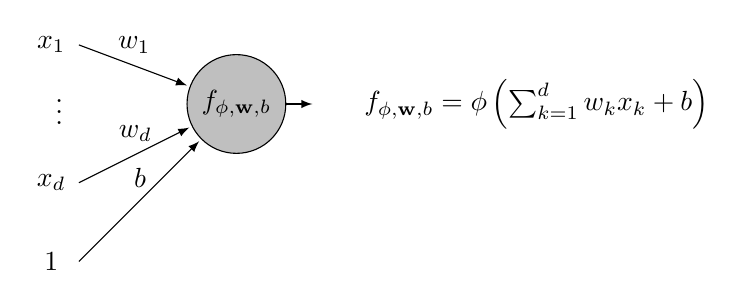
\begin{tikzpicture}[shorten >=1pt,->]
    	\tikzstyle{unit}=[draw,shape=circle,fill=black!25,minimum size=1.15cm]
    
    	\node[unit](p) at (2,1){$f_{\phi, \vec{w}, b}$};
    	\node(dots) at (-0.25,1){\vdots};
    
    	\draw (0,1.75) node[xshift=-10]{$x_1$} -- node[above=0.1em,align=center ] {$w_1$} (p);
    	\draw (0,0) node[xshift=-10]{$x_d$} -- node[above=0.1em,align=center ] {$w_d$} (p);
    	\draw (p) -- (3,1) node[xshift=80]{$f_{\phi, \vec{w}, b} = \phi \left (\sum_{k=1}^d w_k x_k + b \right )$};
    	\draw (0,-1) node[xshift=-10]{$1$} -- node[above=0.1em,align=center ] {$b$}  (p);

	\end{tikzpicture}
    \caption{A neuron parameterized with a weight vector $\vec{w}$, a bias $b$ and an activation function $\phi$. Addition of a bias parameter $b$ is often represented as a "virtual" input $1$ connected to the neuron with a weight of value $b$.}
    \label{fig:neuron}
\end{figure}
The structure and computation of an artificial neuron $f_{\phi, \vec{w}, b}$ is inspired by the structure of the biological neuron. Weights are inspired by synapses and the activation function $\phi$ is used to model the amount of information passed after the neuron processes the input. The model of an artificial neuron has no intention of emulating the much more complex biological counterpart. This analogy is visualized in Figure \ref{fig:neuron}. However, there is a strong connection between linear regression, logistic regression, and the single neuron. For more about linear regression and logistic regression, see Chapter 10 and Chapter 11 in \cite{pmlbook}.
\subsection{Activation functions}
\label{subsection:introduction:dl:activation-functions}
Commonly used activation functions include the logistic sigmoid ($\sigma$), rectified linear unit ($\operatorname{ReLU}$) and hyperbolic tangent ($\tanh$). Less commonly used is the hard binary threshold, also known as the Heaviside step function. However, there are many other activation functions and some of them were invented quite recently. Those include $\operatorname{PReLU}$\cite{he_2015_delving}, $\operatorname{SELU}$\cite{klambauer_2017_selfnormalizing}, $\operatorname{ELU}$\cite{clevert_2015_fast}, $\operatorname{PELU}$\cite{trottier_2018_parametric}. We will present the most commonly used activation functions.
\begin{definition}
The logistic sigmoid $\sigma : \R \to [0,1]$ is given by 
$\sigma(x) = \frac{1}{1 + \exp{(-x)}}$.
\end{definition}

\begin{definition}
The hyperbolic tangent $\tanh : \R \to [-1,1]$ is given by \newline $\tanh{(x)} = \frac{\exp{(x)} - \exp{(-x)}}{\exp{(x)} + \exp{(-x)}}$.
\end{definition}
\begin{definition}
The rectified linear unit $\operatorname{ReLU} : \R \to [0, \infty)$ is given by \newline $\operatorname{ReLU}(x) = \max{(0, x)}$.
\end{definition}
\begin{definition}
The Heaviside step function $s : \R \to \{0,1\}$ is given by
\[ 
    s(x) = \begin{cases} 
      1 & x > 0 \\
      0 & x \leq 0
   \end{cases}.
\]
\end{definition}
\begin{lemma}
\label{lemma:introduction:activation:sigmoid-derivative}
The logistic sigmoid is differentiable on $\R$. Moreover, its derivative satisfies $\frac{\partial \sigma}{\partial x} (x) = \sigma (x) \cdot (1 - \sigma(x)).$
\end{lemma}
\begin{proof}
Let $x \in \R$. Then $\frac{\partial \sigma}{\partial x} (x) = \frac{\exp{(-x)}}{(1 + \exp{(-x)})^2} = \sigma (x) \cdot (1 - \sigma (x)), \text{ as desired. }$
\end{proof}
\begin{figure}[H]
	\centering
	\subfigure[logistic sigmoid ($\sigma$)]{
    		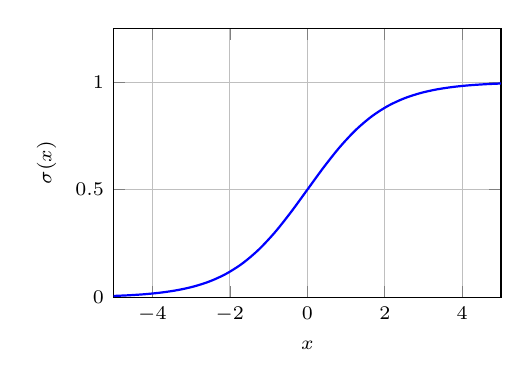
\begin{tikzpicture}
			\begin{axis}[width=6.5cm,height=5cm,ylabel=$\sigma(x)$,xlabel=$x$,ymin=0,ymax=1.25,xmin=-5,xmax=5]
				\addplot[thick,blue,smooth] {1/(1+exp(-x))};
			\end{axis}
		\end{tikzpicture}
	}
	\subfigure[hyperbolic tangent ($\tanh$)]{
		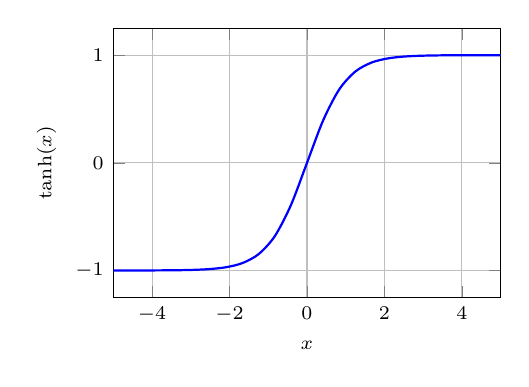
\begin{tikzpicture}
			\begin{axis}[width=6.5cm,height=5cm,ylabel=$\tanh(x)$,xlabel=$x$,ymin=-1.25,ymax=1.25,xmin=-5,xmax=5]
				\addplot[thick,blue,smooth] {tanh(x)};
			\end{axis}
		\end{tikzpicture}
	}\\
	\subfigure[rectified linear unit ($\operatorname{ReLU}$))]{
    		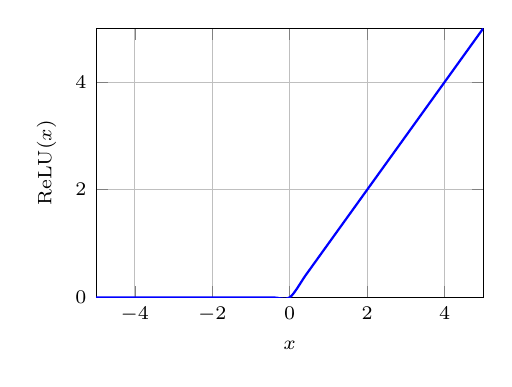
\begin{tikzpicture}
			\begin{axis}[width=6.5cm,height=5cm,ylabel=$\operatorname{ReLU}(x)$,xlabel=$x$,ymin=0,ymax=5,xmin=-5,xmax=5]
				\addplot[thick,blue,smooth] {max(0, x)};
			\end{axis}
		\end{tikzpicture}
	}
	\subfigure[Heaviside step function ($s$)]{
		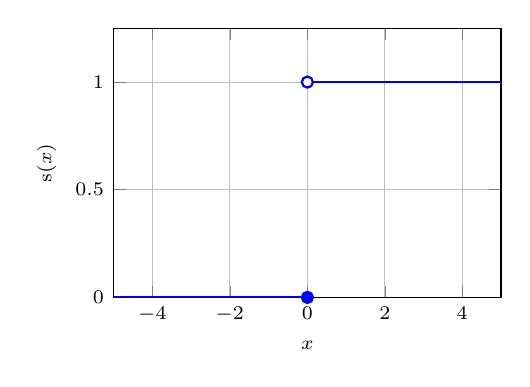
\begin{tikzpicture}
			\begin{axis}[width=6.5cm,height=5cm,ylabel=$\operatorname{s}(x)$,xlabel=$x$,ymin=0,ymax=1.25,xmin=-5,xmax=5]
                \addplot[thick,blue,mark=*,samples at={-100,0}] {0};
                \addplot[thick,blue,mark=*,mark options={fill=white},samples at={0,100}] {1};
			\end{axis}
		\end{tikzpicture}
	}
    	\caption[Commonly used activation functions.]{Commonly used activation functions }
    	\label{fig:introduction:dl:activation-fns}
\end{figure}
\newpage
\subsection{A fully-connected layer}
To perform more complex computations, artificial neurons are often organized to form layers. The following definition will introduce the simplest form of a layer - a \textbf{fully-connected layer}. Many modern neural network layers can be very complex.
\begin{definition}[fully-connected layer]
\label{defn:layer}
A \textbf{fully-connected layer} is a function $f_{\phi, \vec{W}, \vec{b}} : \mathbb{R}^n \to \mathbb{R}^m$ of the form
\begin{equation*}
    f_{\phi, \vec{W}, \vec{b}} (x_1, \ldots, x_n) = \begin{bmatrix}
           f_{\phi, \vec{w_1}, b_1} (x_1, \ldots, x_n)  \\
           f_{\phi, \vec{w_2}, b_2} (x_1, \ldots, x_n) \\
           \vdots \\
           f_{\phi, \vec{w_m}, b_m} (x_1, \ldots, x_n)
         \end{bmatrix},
\end{equation*} where $\vec{W}$ is a matrix of weights corresponding to each neuron in the layer such that $\vec{W}_{i, j}$ is the weight connecting the $i$th input $x_i$ to $j$th neuron in the layer. For $1 \leq k \leq m$, we denote the weight vector of $k$th neuron in the layer by $\vec{w}_k$ and we denote the bias of $k$th neuron in the layer by $b_k$. Hence, weight vectors $\vec{w_1}, \ldots, \vec{w_m}$ are the columns of $\vec{W}$, and layer biases $b_1, \ldots, b_m$ are the components of the bias vector $\vec{b}$. The layer weight matrix $\vec{W}$ and the layer bias vector $\vec{b}$ are given by
\begin{equation*}
    \vec{W} = \begin{bmatrix}
    \vert & \vert  & \vert  & \vert \\
    \vec{w_1}   & \vec{w_2}  & \ldots  & \vec{w_m}   \\
    \vert & \vert & \vert  & \vert
    \end{bmatrix} \text{ and }
    \vec{b} = \begin{bmatrix}
       b_{1}  \\
       b_{2}  \\
       \vdots \\
       b_{m}
    \end{bmatrix}.
\end{equation*}
\end{definition}
\begin{figure}[H]
	\centering
    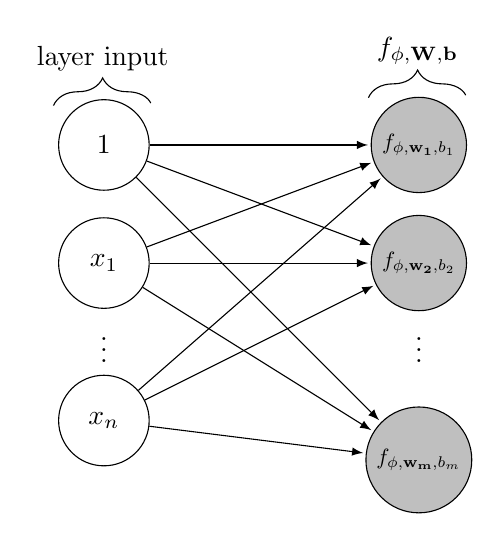
\begin{tikzpicture}[shorten >=1pt]
        \tikzstyle{unit}=[draw,shape=circle,minimum size=1.15cm, scale=0.8,fill=black!25]
        \tikzstyle{input}=[draw,shape=circle,minimum size=1.15cm]

        \node[input](x0) at (0,3.5){$1$};
        \node[input](x1) at (0,2){$x_1$};
        \node(dots) at (0,1){\vdots};
        \node[input](xd) at (0,0){$x_n$};
 
        \node[unit](y1) at (4,3.5){$f_{\phi, \vec{w_1}, b_1}$};
        \node[unit](y2) at (4,2){$f_{\phi, \vec{w_2}, b_2}$};
        \node(dots) at (4,1){\vdots};
        \node[unit](yc) at (4,-0.5){$f_{\phi, \vec{w_m}, b_m}$};
        
        \draw[->] (x0) -- (y1);
        \draw[->] (x0) -- (y2);
        \draw[->] (x0) -- (yc);
 
        \draw[->] (x1) -- (y1);
        \draw[->] (x1) -- (y2);
        \draw[->] (x1) -- (yc);
 
        \draw[->] (xd) -- (y1);
        \draw[->] (xd) -- (y2);
        \draw[->] (xd) -- (yc);
 
        \draw [decorate,decoration={brace,amplitude=10pt},xshift=-4pt,yshift=0pt] (-0.5,4) -- (0.75,4) node [black,midway,yshift=+0.6cm]{layer input};
        \draw [decorate,decoration={brace,amplitude=10pt},xshift=-4pt,yshift=0pt] (3.5,4.1) -- (4.75,4.1) node [black,midway,yshift=+0.6cm]{$f_{\phi, \vec{W}, \vec{b}}$};
    \end{tikzpicture}
    \caption[Network graph of a fully-connected layer with $n$-dimensional input units and $m$-dimensional output.]{A fully-connected layer with $n$-dimensional input and $m$-dimensional output, parameterized with a weight matrix $\vec{W}$, bias vector $\vec{b}$ and an activation function $\phi$. For the sake of clarity, weight and bias labels are omitted. }
    \label{fig:layer}
\end{figure}
\begin{remark}
The layer $f_{\phi, \vec{W}, \vec{b}}$ is often written in the more succint, matrix form
\begin{equation*}
    f_{\phi, \vec{W}, \vec{b}} (\vec{x}) = \phi(\vec{W}^\top \vec{x} + \vec{b}).
\end{equation*}
The application of $\phi$ is understood component-wise. 
\end{remark}
\begin{definition}
We define the \textbf{width} of a layer to be the number of neurons in the layer. Equivalently, the width of a layer is the dimension of the layer output.
\end{definition}
\subsection{A fully-connected neural network}
We are ready to introduce a fully-connected neural network, which is central to this thesis.
\begin{definition}[fully-connected neural network]
\label{defn:nn}
A \textbf{fully-connected neural network} of depth $L$ is a composition of $L$ fully-connected layers. Suppose that the first layer is a function $f_{\phi_1, \vec{W_1}, \vec{b_1}}^{(1)} : \mathbb{R}^{n_{(0)}} \to \mathbb{R}^{n_{(1)}}$ and the last layer is a function $f_{\phi_L, \vec{W_L}, \vec{b_L}}^{(L)} : \mathbb{R}^{n_{(L-1)}} \to \mathbb{R}^{n_{(L)}}$. Suppose that for $1 \leq k \leq L$, the $k$-th layer is a function $f_{\phi_k, \vec{W_k}, \vec{b_k}}^{(k)} : \mathbb{R}^{n_{(k-1)}} \to \mathbb{R}^{n_{(k)}}$. Now, a \textbf{fully-connected neural network} is a composite function parameterized by $L$ layer weight matrices $\{ \vec{W_k}  \}_{k=1}^{L}$, $L$ layer bias vectors $\{ \vec{b_k} \}_{k=1}^{L}$ and $L$ choices of layer activation functions $\{ \phi_{k} \}_{k=1}^{L}$ of the form
\begin{equation*}
    f = f_{\phi_L, \vec{W_L}, \vec{b_L}}^{(L)} \circ  f_{\phi_{(L-1)}, \vec{W_{(L-1)}}, \vec{b_{(L-1)}}}^{(L - 1)} \circ \ldots \circ f_{\phi_1, \vec{W_1}, \vec{b_1}}^{(1)}.
\end{equation*}
\end{definition}
\begin{figure}[H]
	\centering
	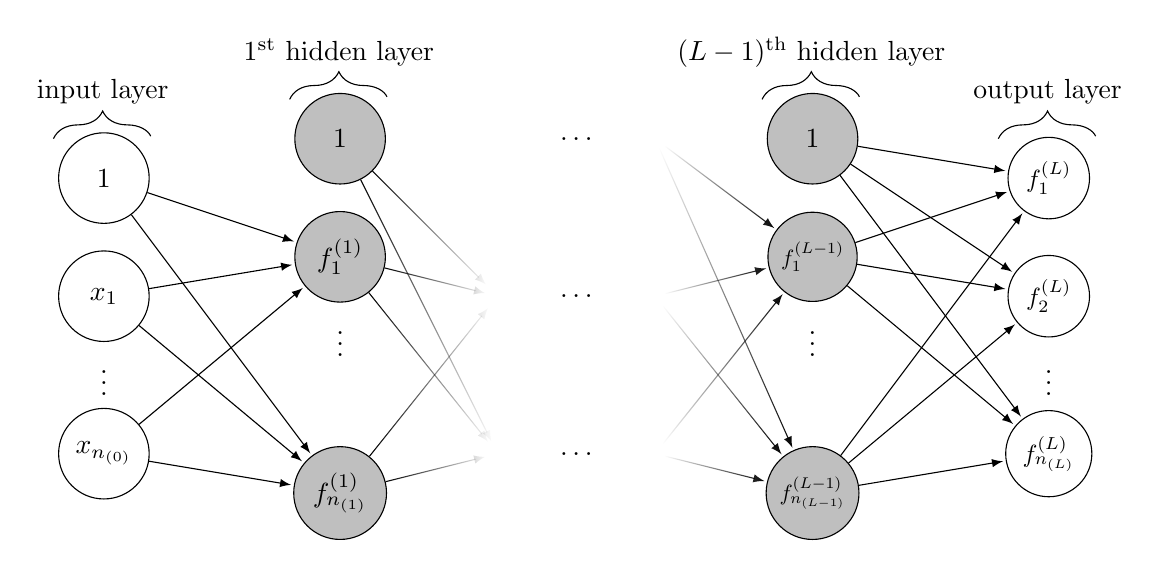
\begin{tikzpicture}[shorten >=1pt]
		\tikzstyle{unit}=[draw,shape=circle,minimum size=1.15cm]
		\tikzstyle{output}=[draw,shape=circle,minimum size=1.15cm,scale=0.9]
		\tikzstyle{hidden}=[draw,shape=circle,fill=black!25,minimum size=1.15cm]
 		\tikzstyle{lasthidden}=[draw,shape=circle,fill=black!25,minimum size=1.15cm,scale=0.8]

		\node[unit](x0) at (0,3.5){$1$};
		\node[unit](x1) at (0,2){$x_1$};
		\node at (0,1){\vdots};
		\node[unit](xd) at (0,0){$x_{n_{(0)}}$};
 
		\node[hidden](h10) at (3,4){$1$};
		\node[hidden](h11) at (3,2.5){$f_{1}^{(1)}$};
		\node at (3,1.5){\vdots};
		\node[hidden](h1m) at (3,-0.5){$f_{n_{(1)}}^{(1)}$};
 
		\node(h22) at (5,0){};
		\node(h21) at (5,2){};
		\node(h20) at (5,4){};
		
		\node(d3) at (6,0){$\ldots$};
		\node(d2) at (6,2){$\ldots$};
		\node(d1) at (6,4){$\ldots$};
 
		\node(hL12) at (7,0){};
		\node(hL11) at (7,2){};
		\node(hL10) at (7,4){};
		
		\node[hidden](hL0) at (9,4){$1$};
		\node[lasthidden](hL1) at (9,2.5){$f_1^{(L-1)}$};
		\node at (9,1.5){\vdots};
		\node[lasthidden](hLm) at (9,-0.5){$f_{n_{(L-1)}}^{(L-1)}$};
 
		\node[output](y1) at (12,3.5){$f_{1}^{(L)}$};
		\node[output](y2) at (12,2){$f_{2}^{(L)}$};
		\node at (12,1){\vdots};	
		\node[output](yc) at (12,0){$f_{n_{(L)}}^{(L)}$};
 
		\draw[->] (x0) -- (h11);
		\draw[->] (x0) -- (h1m);
 
		\draw[->] (x1) -- (h11);
		\draw[->] (x1) -- (h1m);
 
		\draw[->] (xd) -- (h11);
		\draw[->] (xd) -- (h1m);
 
		\draw[->] (hL0) -- (y1);
		\draw[->] (hL0) -- (yc);
		\draw[->] (hL0) -- (y2);
 
		\draw[->] (hL1) -- (y1);
		\draw[->] (hL1) -- (yc);
		\draw[->] (hL1) -- (y2);
 
		\draw[->] (hLm) -- (y1);
		\draw[->] (hLm) -- (y2);
		\draw[->] (hLm) -- (yc);
 
		\draw[->,path fading=east] (h10) -- (h21);
		\draw[->,path fading=east] (h10) -- (h22);
		
		\draw[->,path fading=east] (h11) -- (h21);
		\draw[->,path fading=east] (h11) -- (h22);
		
		\draw[->,path fading=east] (h1m) -- (h21);
		\draw[->,path fading=east] (h1m) -- (h22);
		
		\draw[->,path fading=west] (hL10) -- (hL1);
		\draw[->,path fading=west] (hL11) -- (hL1);
		\draw[->,path fading=west] (hL12) -- (hL1);
		
		\draw[->,path fading=west] (hL10) -- (hLm);
		\draw[->,path fading=west] (hL11) -- (hLm);
		\draw[->,path fading=west] (hL12) -- (hLm);
		
		\draw [decorate,decoration={brace,amplitude=10pt},xshift=-4pt,yshift=0pt] (-0.5,4) -- (0.75,4) node [black,midway,yshift=+0.6cm]{input layer};
		\draw [decorate,decoration={brace,amplitude=10pt},xshift=-4pt,yshift=0pt] (2.5,4.5) -- (3.75,4.5) node [black,midway,yshift=+0.6cm]{$1^{\text{st}}$ hidden layer};
		\draw [decorate,decoration={brace,amplitude=10pt},xshift=-4pt,yshift=0pt] (8.5,4.5) -- (9.75,4.5) node [black,midway,yshift=+0.6cm]{$(L-1)^{\text{th}}$ hidden layer};
		\draw [decorate,decoration={brace,amplitude=10pt},xshift=-4pt,yshift=0pt] (11.5,4) -- (12.75,4) node [black,midway,yshift=+0.6cm]{output layer};
	\end{tikzpicture}
	\caption[Network graph for a $(L+1)$-layer fully-connected neural network.]{Network graph of a $L$-layer fully-connected neural network with $n_{(0)}$-dimensional input and $n_{(L)}$-dimensional output. This illustration corresponds to Definition \ref{defn:nn}. The $k^{\text{th}}$ hidden layer contains $n_{(k)}$ neurons for $1 \leq k \leq L$. For the sake of clarity, parameters $\vec{W_k}, \vec{b_k}$ and activation functions $\phi_k$ are omitted from the graph. Hence, $f_{j}^{(k)}$ in the graph represents $(f_{\phi_k, \vec{W_k}, \vec{b_k}})_j$, in the sense of Definition \ref{defn:layer}.}
	\label{fig:nn}
\end{figure}
In literature, the layers $f_{\phi_k, \vec{W_k}, \vec{b_k}} : \mathbb{R}^{n_{(k-1)}} \to \mathbb{R}^{n_{k}}$, for $1 \leq k \leq L$ are often called $\textbf{hidden or latent layers}$. To analyse interactions between layers, we will often decompose $f_{\phi^{(k)}, \vec{W}^{(k)}, \vec{b}^{(k)}}$ into the computation of the affine transformation and the application of the activation function,  \begin{align*}
    f_{\phi^{(k)}, \vec{W}^{(k)}, \vec{b}^{(k)}} (\vec{x}) = \phi^{(k)} (\vec{a}^{(k)}(\vec{x})) \text{ where } \vec{a}^{(k)} (\vec{x})  = (\vec{W}^{(k)})^{\top}\vec{x} + \vec{b}^{(k)}.
\end{align*}

\section{Forward pass}
Let $\vec{f} : \R^{n_{(0)}} \to \R^{n_{(L)}}$ be an $L$-layer fully-connected neural network parameterized by $L$ weight matrices $\{ \vect{W}^{(l)}  \}_{l=1}^{L}$, bias vectors $\{  \vect{b}^{(l)} \}_{l=1}^{L}$ and choices of activation functions $\{ \sigma^{(l)} \}_{l=1}^{L}$. 
To evaluate predictions of the neural network $\vec{f}$ on input $\vec{x} \in \R^n$, we set $\vec{f}^{(0)} = \vec{x}$ and repeatedly evaluate following equations
\begin{subequations}
\begin{align}
    \vec{a}^{(l)} &= (\vec{W}^{(l)})^{\top} \vec{f}^{(l - 1)} + \vec{b}^{(l)}, \text{ for $1 \leq l \leq L$}, \label{eqn:introduction:forward:vectorised:a}  \\
    \vec{f}^{(l)} &= \sigma ^{(l)}(\vec{a}^{(l)}), \text{ for $1 \leq l \leq L$}. \label{eqn:introduction:forward:vectorised:f}
\end{align}
\end{subequations}
Equations \ref{eqn:introduction:forward:vectorised:a} and \ref{eqn:introduction:forward:vectorised:f} are componentwise equivalent to
\begin{subequations}
\begin{align}
    a_{i}^{(l)} &= \sum_{k = 1}^{n_{(l-1)}} w_{ki}^{(l)} f_{k}^{(l-1)} + b^{(l)}_i, \text{ for $1 \leq i \leq n^{(l)}$,} \label{eqn:introduction:forward:explicit:a} \\
    f^{(l)}_{i} &= \sigma ^{(l)}(a_{i}^{(l)}), \text{ for $1 \leq i \leq n^{(l)}$.} \label{eqn:introduction:forward:explicit:f}
\end{align}
\end{subequations}
The process of evaluating $\vec{f}$ on input $\vec{x}$ is known as the forward pass. 
\section{Gradient descent and backpropagation algorithm}
One of the most important ideas in machine learning is expressing the learning problem as an optimization problem. In this thesis, we will discuss only the supervised learning approach.
In the supervised setting, we define a \textbf{loss function}, which is a function measuring the error between predictions of the model given the input and correct label corresponding to the input on which the model was evaluated. 
Assuming fixed neural network topology and a fixed choice of activation functions per layer, in the language of subsection \ref{subsection:ml:terminology}, neural networks are a family of hypothesis functions, parameterized by weights and biases. The purpose of the backpropagation learning algorithm is to find the configuration of weights and biases corresponding to the minimal loss on the training set, using the method of gradient descent. Gradient descent is a first-order, iterative optimization algorithm based on the following fact from analysis in $\R^n$.
\begin{claim}
If the multivariable differentiable function $\vec{f}: \R^n \to \R$ is defined and differentiable in a neighbourhood of $\vec{a} \in \R^n$, then $\vec{f}$ decreases fastest at $\vec{a}$ in direction $-\nabla f(\vec{a})$ from $\vec{a}$.
\end{claim}
In gradient descent, the claim above is applied to the loss function. In this context, the loss function is a function of parameters of the neural network. The loss function is evaluated on the entire training set or its subset. Those parameters are $L$ layer weight matrices $\{ \vec{W}_l \}_{l=1}^L$ and $L$ layer bias vectors $\{ \vec{b}_l \}_{l=1}^L$.
Gradient descent iteratively refines the current configuration of weights and biases by moving in the direction in the parameter space suggested by the claim above. This heuristic is expressed as equations \ref{eqn:introduction:backprop:unvectorised_eqn_W_t} and \ref{eqn:introduction:backprop:unvectorised_eqn_b_t}, discussed on the next page.
\newpage
In our context, gradient descent is implemented by the following iterative process, repeated for a fixed number of steps or until convergence,
\begin{subequations}
\begin{align}
    w_{ij}^{(l)} [t + 1] &= w_{ij}^{(l)} [t] - \eta \frac{\partial \mathcal{L} }{\partial w_{ij}^{(l)}[t]} \label{eqn:introduction:backprop:unvectorised_eqn_W_t} \\ 
    b_{j}^{(l)} [t + 1] &= b_{j}^{(l)} [t] - \eta  \frac{\partial \mathcal{L} }{\partial b_{j}^{(l)}[t]}, \label{eqn:introduction:backprop:unvectorised_eqn_b_t} 
\end{align}
\end{subequations}
where $\eta > 0$ is a small constant known as \textbf{the learning rate}. The index $[t]$ indicates the current training step.
Equations \ref{eqn:introduction:backprop:unvectorised_eqn_W_t} and \ref{eqn:introduction:backprop:unvectorised_eqn_b_t} can be expressed in the following vectorised form.
\begin{subequations}
\begin{align}
    \vec{W}^{(l)}[t + 1] &= \vec{W}^{(l)}[t] - \eta \frac{\partial \mathcal{L}}{\partial \vec{W}^{(l)}[t]}, \label{eqn:introduction:backprop:vectorised_eqn_W_t} \\ 
    \vec{b}^{(l)}[t + 1] &= \vec{b}^{(l)}[t] - \eta \frac{\partial \mathcal{L}}{\partial \vec{b}^{(l)}[t]}. \label{eqn:introduction:backprop:vectorised_eqn_b_t}
\end{align}
\end{subequations}
There are indeed many ways to initialize weights and biases. The initialization of weights and biases may significantly affect the gradient descent performance, especially in the case of sigmoidal activation functions. An example of a problem related to the initialization of weights and biases is the problem of \textit{vanishing gradients}. We will briefly discuss initialization methods presented in \cite{glorot_understanding} and \cite{he_2015_delving}. However, many different methods exist and are used in practice. For sigmoidal and symmetric activation functions, a common initialization method is \textit{ Xavier/Glorot initialization} \cite{glorot_understanding},
\begin{align*}
     w_{ij}^{(l)} [0] \sim \mathcal{U} \left (-\sqrt{\frac{6}{n_{(l)} + n_{(l - 1)}}}, \sqrt{\frac{6}{n_{(l)} + n_{(l - 1)}}}  \right ).
\end{align*}
When it comes to rectified activation functions, more prevalent initialization method is \textit{He initialization} \cite{he_2015_delving},
\begin{align*}
     w_{ij}^{(l)} [0] \sim \mathcal{N} \left (0, \sqrt{\frac{2}{n_{(l-1)}}} \right).
\end{align*}
Biases are often zero-initialized. Due to the structure of feed-forward neural networks and nonlinearity induced by activation functions, minimizing the training set loss is often not a convex optimization problem. Hence the gradient-based optimization presented above may not converge to a global minimum (if it exists) or even converge at all. However, this method works surprisingly well in practice and it recently became a topic of active research. 
For instance, \cite{li_2018_visualizing} has recently provided a method to visualize loss surfaces of modern neural networks. Using those visualizations, the paper provided a possible explanation of the trainability of modern deep networks. Until recently, it was thought that gradient-based optimization may struggle with local optima and saddle points. Although this is theoretically possible, it seems that optimizers work well in practice. \newpage Many of the latest papers often use more sophisticated gradient-based optimizers. Those optimizers are designed to mitigate common problems related to gradient-based optimization, such as the performance on plateaus. Such optimizers are Adam, Nadam, Nesterov Accelerated Gradient, Adagrad, Adadelta, and RMSProp. For a comprehensive overview of those methods see \cite{ruder_2017_an}.
\subsection{Stochastic and batch gradient descent}
Since the training set can often be quite large, it quickly becomes computationally infeasible to compute gradients $\frac{\partial \mathcal{L}}{\partial \vec{W}^{(l)}[t]}, \frac{\partial \mathcal{L}}{\partial \vec{b}^{(l)}[t]}$. This problem arises if the loss function $\mathcal{L}$ is evaluated on the entire training set. A very common solution to this problem is to use stochastic gradient descent or batch gradient descent. Batch gradient descent procedure divides the training of the network into epochs. In each epoch, a small sample is sampled from the training set. This sampled subset of the training set is called a training \textbf{batch}. The loss function is evaluated with respect to the batch and equations \ref{eqn:introduction:backprop:vectorised_eqn_W_t}, \ref{eqn:introduction:backprop:vectorised_eqn_b_t} are also computed with respect to the batch. Stochastic gradient descent is a name for batch gradient descent when a training batch consists of precisely one training example.

\subsection{Loss functions}
To discuss loss functions, let $\vec{f} : \R^{n_{(0)}} \to \R^{n_{(L)}}$ be an $L$-layer fully-connected neural network parameterized by $L$ weight matrices $\{ \vect{W}^{(l)}  \}_{l=1}^{L}$, bias vectors $\{  \vect{b}^{(l)} \}_{l=1}^{L}$ and choices of activation functions $\{ \sigma^{(l)} \}_{l=1}^{L}$. Suppose $\{ (\vec{x}_k, \vec{y}_k) \}_{k=1}^n$ is the training set. The choice of the loss function depends on the type of a problem that the network $\vec{f}$ is designed to solve.
The mean square error is widely-used for regression problems. In this setting, the output layer often has identity activation.
\begin{definition}[mean square error loss]
The square loss corresponding to the single training item $ (\vec{x}_k, \vec{y}_k)$ is given by 
\begin{align*}
    \mathcal{L}_{k}(\{ \vec{W}^{(l)} \}_{l=1}^{L},\{ \vec{b}^{(l)} \}_{l=1}^{L}) = \frac{1}{2} \norm{\vec{f}(\vec{x}_k) - \vec{y_k}}^{2}_2 = \frac{1}{2} \sum_{j = 1}^{n_{(L)}} (f^{(L)}_{j}(\vec{x}_k) - y_{k_{j}})^{2}.
\end{align*}
The mean square loss of the training set is given by
\begin{align*}
    \mathcal{L}(\{ \vec{W}^{(l)} \}_{l=1}^{L},\{ \vec{b}^{(l)} \}_{l=1}^{L}) &= \frac{1}{n} \sum_{k = 1}^n  \mathcal{L}_{k}(\{ \vec{W}^{(l)} \}_{l=1}^{L},\{ \vec{b}^{(l)} \}_{l=1}^{L} ) \\ 
    &= \frac{1}{2n} \sum_{k = 1}^n  \norm{\vec{f}(\vec{x}_k) - \vec{y_k}}^{2}_2 \\
    &=  \frac{1}{2n} \sum_{k = 1}^n \sum_{j = 1}^{n_{(L)}} (f^{(L)}_{j}(\vec{x}_k) - y_{k_{j}})^{2}.
\end{align*}
\end{definition}
\pagebreak
We will briefly discuss neural networks for multi-class classification. In this setting, we usually design a neural network such that its output layer width matches the number of different classes. Hence, each output layer neuron represents a class.
Although it is possible to use the mean square error loss to train neural networks for classification, it is often a better idea to use the categorical cross-entropy loss. Categorical cross-entropy loss is a loss function designed for classification problems. In classification setting, this loss is theoretically superior to the mean squared error. For instance, it is tightly connected to Kullback-Leibler divergence between true class distribution and the class distribution the model is designed to learn. The cross-entropy loss is particularly effective when the last layer of the neural network implements \textit{softmax}\cite{bridle_training} activation function.
\begin{definition}[categorical cross-entropy loss]
The cross entropy loss corresponding to $(\vec{x}_k, \vec{y}_k)$ is given by 
\begin{align*}
    \mathcal{L}_{k}(\{ \vec{W}^{(l)} \}_{l=1}^{L},\{ \vec{b}^{(l)} \}_{l=1}^{L}) = - \sum_{j=1}^{n_{(L)}} y_{k_{j}} \ln{{f}^{(L)}_j(\vec{x}_k) }.
\end{align*}
The cross entropy loss of the training set is given by
\begin{align*}
    \mathcal{L}(\{ \vec{W}^{(l)} \}_{l=1}^{L},\{ \vec{b}^{(l)} \}_{l=1}^{L}) &= \sum_{k = 1}^n \mathcal{L}_{k}(\{ \vec{W}^{(l)} \}_{l=1}^{L},\{ \vec{b}^{(l)} \}_{l=1}^{L} ) \\ 
                                                                             &= \sum_{k = 1}^n \sum_{j=1}^{n_{(L)}} y_{k_{j}} \ln{f^{(L)}_j(\vec{x}_k) }.
\end{align*}
\end{definition}
\section{Backward pass}
In this section, we will show how to systematically compute gradients \ref{eqn:introduction:backprop:vectorised_eqn_W_t} and \ref{eqn:introduction:backprop:vectorised_eqn_b_t} of any differentiable loss function for any fully-connected neural network. For the sake of brevity, we will denoted the $l$th layer of a neural network by $\vec{f}^{(l)}$.
\begin{proposition}[Backpropagation equations]
\label{proposition:introduction:backward:naive}
Let $\vec{f} : \R^{n_{(0)}} \to \R^{n_{(L)}}$ be a differentiable, fully-connected neural network of $L$ layers, parameterized by $L$ weight matrices $\{ \vect{W}^{(l)}  \}_{l=1}^{L}$, bias vectors $\{  \vect{b}^{(l)} \}_{l=1}^{L}$ and choices of activation functions $\{ \sigma^{l} \}_{l=1}^{L}$.
Let $\mathcal{L}$ be a differentiable loss function for a single example $(\vec{x}, \vec{y})$, so $\vec{f}^{(0)} = \vec{x}$. Then
\begin{subequations}
\begin{align}
    \frac{\partial \mathcal{L}}{\partial w_{ij}^{(l)}} &= \delta_j^{l} \cdot f_{i}^{(l-1)}, \text{ for every $1 \leq i \leq n_{(l-1)}$}, 1 \leq j \leq n_{(l)},  \label{eqn:introduction:proposition:backward:naive:partial_L_partial_wij} \\
    \frac{\partial \mathcal{L}}{\partial b_{j}^{(l)}}  &= \delta_j^{l}, \text{ for every } 1 \leq j \leq n_{(l)}, 1 \leq l \leq L,  \label{eqn:introduction:proposition:backward:naive:partial_L_partial_b_j} \\
    \delta_i^{(l-1)} &= \left (\sum_{j=1}^{n_{(l)}}  \delta_j^{(l)} w_{ij}^{(l)} \right) \cdot \left(\sigma^{(l-1)}\right){'} ( a_{i}^{(l-1)}), \text{ for } 1 \leq i \leq n_{(l-1)},  1 \leq l \leq L,  \label{eqn:introduction:proposition:backward:naive:delta_l_minus_1}  \\ 
    \delta_i^{(L )} &= \frac{\partial \mathcal{L}}{\partial f_{i}^{(L)}} \cdot \left(\sigma^{(L)}\right){'} ( a_{i}^{(L)}), \text{ for } 1 \leq i \leq n_{(L)}. \label{eqn:introduction:proposition:backward:naive:delta_L}  
\end{align}
\end{subequations}
\end{proposition}
\begin{proof}
\setcounter{step}{0}
\begin{step}[Computation of $\frac{\partial \mathcal{L}}{\partial w_{ij}^{(l)}}, \frac{\partial \mathcal{L}}{\partial b_{i}^{(l)}}$]
Let $\mathcal{L}$ be a loss function, as in the statement. We are interested in quantitites $\frac{\partial \mathcal{L}}{\partial w_{ij}^{(l)}}$ \text{ and } $\frac{\partial \mathcal{L}}{\partial b_{i}^{(l)}}$. Consider single weight $w_{ij}^{(l)}$. By Definition \ref{defn:nn}, the weight $w_{ij}^{(l)}$ connects $i$th neuron in $(l - 1)$th layer to $j$th neuron in $(l)$th layer. By \ref{eqn:introduction:forward:explicit:a}, the weight $w_{ij}^{(l)}$ contributes only to $a_j^{(l)}$ and no other component of $\vec{a}^{(l)}$. Now consider a single bias component $b_{j}^{(l)}$. By \ref{eqn:introduction:forward:explicit:a}, the bias component $b_{j}^{(l)}$ contributes only to $a_j^{(l)}$ and no other component of $\vec{a}^{(l)}$. Thus, by the Chain Rule, \begin{align}
    \label{eqn:introduction:backward:partial_c_partial_wij_bj}
    \frac{\partial \mathcal{L}}{\partial w_{ij}^{(l)}} = \frac{\partial \mathcal{L}}{\partial a_{j}^{(l)}} \cdot  \frac{\partial a_{j}^{(l)}}{\partial w_{ij}^{(l)}} \text{ and }     \frac{\partial \mathcal{L}}{\partial b_{j}^{(l)}} = \frac{\partial \mathcal{L}}{\partial a_{j}^{(l)}} \cdot  \frac{\partial a_{j}^{(l)}}{\partial b_{j}^{(l)}}.
\end{align}
Consider $\frac{\partial a_{j}^{(l)}}{\partial w_{ij}^{(l)}}$ and $\frac{\partial a_{j}^{(l)}}{\partial b_{j}^{(l)}}$. By \ref{eqn:introduction:forward:explicit:a}, \begin{align}
    \label{eqn:introduction:backward:partial_alpha_j_partial_wij_bj}
    \frac{\partial a_{j}^{(l)}}{\partial w_{ij}^{(l)}} &= \frac{\partial}{\partial w_{ij}^{(l)}} \left (  \sum_{k = 1}^{n_{(l-1)}} w_{kj}^{(l)} f_{k}^{(l-1)} + b^{(l)}_j \right ) = f_{i}^{(l-1)}, \\
    \frac{\partial a_{j}^{(l)}}{\partial b_{j}^{(l)}} &= \frac{\partial}{\partial b_{j}^{(l)}} \left (  \sum_{k = 1}^{n_{(l-1)}} w_{kj}^{(l)} f_{k}^{(l-1)} + b^{(l)}_j \right ) = 1.
\end{align}
Substituting \ref{eqn:introduction:backward:partial_alpha_j_partial_wij_bj} into \ref{eqn:introduction:backward:partial_c_partial_wij_bj} gives \begin{align}
    \label{eqn:introduction:backward:partial_c_partial_wij_bij_2}
    \frac{\partial \mathcal{L}}{\partial w_{ij}^{(l)}} = \frac{\partial \mathcal{L}}{\partial a_{j}^{(l)}} \cdot f_{i}^{(l-1)}, \text{ and }
    \frac{\partial \mathcal{L}}{\partial b_{j}^{(l)}} = \frac{\partial \mathcal{L}}{\partial a_{j}^{(l)}}.
\end{align}
\end{step}
For the sake of simplicity, set $\delta_j^{(l)} = \frac{\partial \mathcal{L}}{\partial a_{j}^{(l)}}$.
Then by \ref{eqn:introduction:backward:partial_c_partial_wij_bij_2}
\begin{align}
    \frac{\partial \mathcal{L}}{\partial w_{ij}^{(l)}} = \delta_j^{l} \cdot f_{i}^{(l-1)}  \text{ and }
    \frac{\partial \mathcal{L}}{\partial b_{j}^{(l)}}  = \delta_j^{l}.
\end{align}
By \ref{eqn:introduction:backward:partial_c_partial_wij_bij_2}, to compute $\frac{\partial \mathcal{L}}{\partial w_{ij}^{(l)}}, \frac{\partial \mathcal{L}}{\partial b_{j}^{(l)}}$, it remains to compute $\delta_j$.

\begin{step}[Computation of $\delta_j$]
We begin with $\delta_L$. By the Chain Rule, \begin{align*}
    \delta_i ^{(L)} = \frac{\partial \mathcal{L}}{\partial f_{i}^{(L)}} \cdot \frac{\partial f_{i}^{(L)}}{\partial a_{i}^{(L)}}, \text{ for $1 \leq i \leq n_{(L)}$}.
\end{align*}
Now consider $\frac{\partial f_{i}^{(L)}}{\partial a_{i}^{(L)}}$. Differentiating \ref{eqn:introduction:forward:explicit:f} yields \begin{align}
    \frac{\partial f_{i}^{(L)}}{\partial a_{i}^{(L)}}= \frac{\partial}{\partial a_{i}^{(L)}} \left ( \sigma^{(L)}(a_{i}^{(L)}) \right ) =  (\sigma^{(L)})^{'}(a_{i}^{(L)}).
\end{align}
We will express $\delta_i^{(l-1)} $ in terms of $\delta_j^{(l)}$. By \ref{eqn:introduction:forward:explicit:a} and \ref{eqn:introduction:forward:explicit:f}, for every $1 \leq i \leq n_{(l-1)}$, $a_i^{(l - 1)}$ contributes to the value of every $a_j^{(l)}$ via $f_i^{(l-1)}$ and only via $f_i^{(l-1)}$. This relationship can be easily seen in Figure \ref{fig:introduction:backprop:between-successive-layers}. By the Chain Rule, for every  $1 \leq l \leq L$, for every $1 \leq i \leq n_{(l-1)}$, 
\begin{subequations}\label{eqn:introduction:backward:delta_i}
\begin{align*}
   \delta_i^{(l-1)} = \frac{\partial \mathcal{L}}{\partial a_{i}^{(l - 1)}} &= \sum_{j=1}^{n_{(l)}} \frac{\partial \mathcal{L}}{\partial a_{j}^{(l)}} \cdot \frac{\partial a_{j}^{(l)}}{\partial a_{i}^{(l-1)}} \\  &= \sum_{j=1}^{n_{(l)}} \delta_j^{(l)}   \cdot \frac{\partial a_{j}^{(l)}}{\partial a_{i}^{(l-1)}}. \tag{\ref{eqn:introduction:backward:delta_i}}
\end{align*}
\end{subequations}

\noindent\begin{minipage}{0.25\textwidth}% adapt widths of minipages to your needs
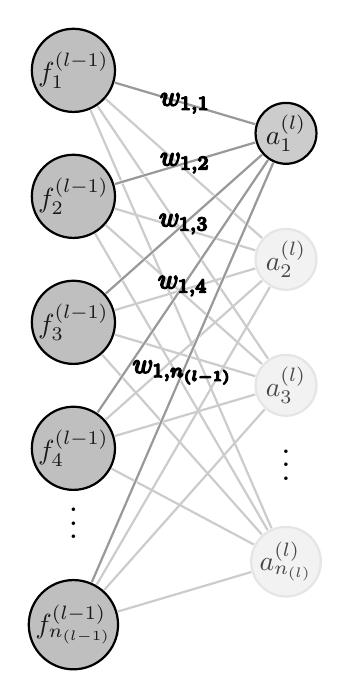
\begin{tikzpicture}[x=2.7cm,y=1.6cm]
  \def\NI{5} % number of nodes in input layers
  \def\NO{4} % number of nodes in output layers
  \def\yshift{0.4} % shift last node for dots
  
  % INPUT LAYER
  \foreach \i [evaluate={\c=int(\i==\NI); \y=\NI/2-\i-\c*\yshift; \index=(\i<\NI?int(\i):"n_{(l-1)}");}]
              in {1,...,\NI}{ % loop over nodes
    \node[node in,outer sep=0.6] (NI-\i) at (0,\y) {$f_{\index}^{(l-1)}$};
  }
  
  % OUTPUT LAYER
  \foreach \i [evaluate={\c=int(\i==\NO); \y=\NO/2-\i-\c*\yshift; \index=(\i<\NO?int(\i):"n_{(l)}");}]
    in {\NO,...,1}{ % loop over nodes
    \ifnum\i=1 % high-lighted node
      \node[node hidden]
        (NO-\i) at (1,\y) {$a_{\index}^{(l)}$};
      \foreach \j [evaluate={\index=(\j<\NI?int(\j):"n_{(l-1)}");}] in {1,...,\NI}{ % loop over nodes in previous layer
        \draw[connect,white,line width=1.2] (NI-\j) -- (NO-\i);
        \draw[connect,mygray!40] (NI-\j) -- (NO-\i)
          node[pos=0.50,mydarkgray] {\contour{black}{$w_{1,\index}$}};
      }
    \else % other light-colored nodes
      \node[node,gray!20!black!80,draw=mygray!10,fill=mygray!5]
        (NO-\i) at (1,\y) {$a_{\index}^{(l)}$};
      \foreach \j in {1,...,\NI}{ % loop over nodes in previous layer
        %\draw[connect,white,line width=1.2] (NI-\j) -- (NO-\i);
        \draw[connect,mygray!20] (NI-\j) -- (NO-\i);
      }
    \fi
  }
  
  % DOTS
  \path (NI-\NI) --++ (0,1+\yshift) node[midway,scale=1.2] {$\vdots$};
  \path (NO-\NO) --++ (0,1+\yshift) node[midway,scale=1.2] {$\vdots$};
\end{tikzpicture}
\captionof{figure}{between two successive layers $f^{(l-1)}$ and $f^{(l)}$.}
\label{fig:introduction:backprop:between-successive-layers}
\end{minipage}%
\hfill%
\begin{minipage}{0.65\textwidth}
By \ref{eqn:introduction:forward:explicit:a} and \ref{eqn:introduction:forward:explicit:f}, 
\begin{subequations}\label{eqn:introduction:backward:alpha_j}
\begin{align*}
    a_{j}^{(l)} &= \sum_{k = 1}^{n_{(l-1)}} w_{kj}^{(l)} f_{k}^{(l-1)} + b^{(l)}_j \\ 
                     &= \sum_{k = 1}^{n_{(l-1)}} w_{kj}^{(l)} \sigma^{(l-1)}(a_{k}^{(l-1)}) + b^{(l)}_j. \tag{\ref{eqn:introduction:backward:alpha_j}} 
\end{align*}
\end{subequations}
Differentiating \ref{eqn:introduction:backward:alpha_j} with respect to $a_{i}^{(l)}$ gives 
\begin{subequations}\label{eqn:introduction:backward:partial_alpha_j_partial_alpha_i}
\begin{align*}
   \frac{\partial a_{j}^{(l)}}{\partial a_{i}^{(l-1)}} &= \frac{\partial}{\partial a_{i}^{(l-1)}} \left ( \sum_{k = 1}^{n_{(l-1)}} w_{kj}^{(l)} f_{k}^{(l-1)} + b^{(l)}_j \right ) & \\ 
                     &= \frac{\partial}{\partial a_{i}^{(l-1)}} \left ( \sum_{k = 1}^{n_{(l-1)}} w_{kj}^{(l)} \sigma^{(l-1)}(a_{k}^{(l-1)}) + b^{(l)}_j \right ) & \\ 
                     &= w_{ij}^{(l)} \cdot \left(\sigma^{(l-1)}\right){'} ( a_{i}^{(l-1)}). \tag{\ref{eqn:introduction:backward:partial_alpha_j_partial_alpha_i}} 
\end{align*}
\end{subequations}
\end{minipage}
Substituting \ref{eqn:introduction:backward:partial_alpha_j_partial_alpha_i} into \ref{eqn:introduction:backward:delta_i} gives \begin{align*}
    \delta_i^{(l-1)} &= \sum_{j=1}^{n_{(l)}} \delta_j^{(l)} w_{ij}^{(l)} \left(\sigma^{(l-1)}\right){'} ( a_{i}^{(l-1)}) 
                = \left (\sum_{j=1}^{n_{(l)}}  \delta_j^{(l)} w_{ij}^{(l)} \right) \cdot \left(\sigma^{(l-1)}\right){'} ( a_{i}^{(l-1)}).
\end{align*}
\end{step}
\end{proof}
In practice, the standard way of implementing equations from \nameref{proposition:introduction:backward:naive} is an implementation in the vectorized form. Two main advantages of vectorization are readability and performance. Recently, many deep learning programming frameworks started implementing a wide variety of optimized linear algebra routines \cite{li_2020_the}, often supporting efficient execution on GPUs and TPUs. Given the sheer size of modern datasets, vectorization is key to the computationally feasible implementation of both forward and backward passes.
\begin{corollary}[Vectorised backpropagation equations]
\label{corollary:introduction:backprop:vectorised}
\begin{subequations}
\begin{align}
    \frac{\partial \mathcal{L}}{\partial \vec{W}^{(l)}} &= \vec{f}^{(l-1)} \delta^{(l)^{\top}} \label{eqn:backward:vectorised_partial_L_partial_W_l} \\ 
    \frac{\partial \mathcal{L}}{\partial \vec{b}^{(l)}} &= \delta^{(l)} \label{eqn:backward:vectorised_partial_L_partial_b_l} \text{ where } \\
    \delta^{(l-1)} &= \left ( \vec{W}^{(l)} \delta^{(l)} \right ) \odot  \left(\sigma^{(l - 1)}\right){'} ( \vec{a}_{i}^{(l - 1)}) \label{eqn:backward:vectorised_delta_l_minus_1} \text{ , for $1 \leq l \leq L$, }\\ 
    \delta^{(L)} &= \frac{\partial \mathcal{L}}{\partial \vec{f}^{(L)} } \odot  \left(\sigma^{(L)}\right){'} ( \vec{a}^{(L)}). \label{eqn:backward:vectorised_delta_L}
\end{align}
\end{subequations}
\end{corollary}
\begin{remark}
The symbol $\odot$ denotes the elementwise product, known as also Hadamard product.
\end{remark}
\begin{proof}
The claimed equations follow directly from \nameref{proposition:introduction:backward:naive}. Writing \ref{eqn:introduction:proposition:backward:naive:partial_L_partial_wij} in terms of matrix outer product yields \ref{eqn:backward:vectorised_partial_L_partial_W_l}. Vectorizing \ref{eqn:introduction:proposition:backward:naive:partial_L_partial_b_j} yields \ref{eqn:backward:vectorised_partial_L_partial_b_l}.
Recognising the inner product expansion $\sum_{j=1}^{n_{(l)}} \delta_j^{(l)} w_{ij}^{(l)}$ in \ref{eqn:introduction:proposition:backward:naive:delta_l_minus_1} and applying the definition of matrix-vector multiplication $\vec{W}^{(l)} \delta^{(l)}$ yields \ref{eqn:backward:vectorised_delta_l_minus_1}. Vectorizing \ref{eqn:introduction:proposition:backward:naive:delta_L} yields \ref{eqn:backward:vectorised_delta_L}.
\end{proof}

\begin{remark}
It is worth discussing the computational complexity of  \nameref{proposition:introduction:backward:naive}. Recall that the forward pass equations are
\begin{align*}
    \vec{a}^{(l)} &= (\vec{W}^{(l)})^{\top} \vec{f}^{(l - 1)} + \vec{b}^{(l)}, \text{ for $1 \leq l \leq L$,} \\
    \vec{f}^{(l)} &= \sigma ^{(l)}(\vec{a}^{(l)}),  \text{ for $1 \leq l \leq L$,} \\
    \vec{f}^{(0)} &= \vec{x}.
\end{align*}
By comparing those equations to \ref{eqn:backward:vectorised_partial_L_partial_W_l}, \ref{eqn:backward:vectorised_partial_L_partial_b_l},  \ref{eqn:backward:vectorised_delta_L}, \ref{eqn:backward:vectorised_delta_l_minus_1}, it is not difficult to observe that the time complexity of gradient computation is asymptotically equivalent to the time complexity of forward pass. This implies that backpropagation training is as computationally efficient as evaluating neural network predictions. The computational efficiency of backpropagation algorithm is a very important factor in widespread use of neural networks.
\end{remark}

\begin{remark}
We will briefly discuss the importance of the differentiability of the loss function and the neural network. Loss functions are often differentiable, but many modern neural network architectures use rectified activation functions that are not differentiable. This implies that neural networks themselves are not differentiable so the \nameref{proposition:introduction:backward:naive} simply do not hold. However, the gradient descent algorithm can be generalized to the (sub)gradient descent algorithm.
\end{remark}

\begin{remark}
So far, we have discussed only the theoretical foundations for training fully-connected neural networks.
In practice, there is a wide range of software frameworks designed to simplify the design of neural networks and to automate gradient computations we demonstrated in \nameref{proposition:introduction:backward:naive}. Apart from just simplifying gradient computations, modern deep learning software frameworks perform very complex optimizations. The most popular frameworks are Tensorflow\cite{tensorflow2015-whitepaper}, PyTorch \cite{paszke_2019_pytorch} and Jax\cite{jax2018github}. 
We will use PyTorch in \nameref{chapter:experiments}.
\end{remark}

\chapter{Literature review}
\label{chapter:literature-review}

Since the invention of the backpropagation algorithm in \citetitle{rumelhart_1986_learning} \cite{rumelhart_1986_learning}, neural networks have been applied to a wide variety of problems in pattern recognition and machine learning.

\begin{displayquote}[\citetitle{bishop_1998_neural} \cite{bishop_1998_neural}, p.5]
"The importance of neural networks in this context is that they offer a very powerful and very general framework for representing non-linear mappings from several input variables to several output variables, where the form of the mapping is governed by a number of adjustable parameters."
\end{displayquote}
Recently, very sophisticated neural networks began to significantly outperform alternative machine learning methods in a wide variety of tasks, including natural language processing (\cite{vaswani_2017_attention}, \cite{brown_2020_language}), computer vision (\cite{szegedy_2014_going}, \cite{he_2015_deep}, \cite{bochkovskiy_2020_yolov4}), computational biology (\cite{senior_2020_improved}) and reinforcement learning (\cite{silver_2017_mastering}). Interestingly, some of the most influential researchers in the field received a Turing award for their work in deep learning. However, most of the advancements in the field came from clever architectures, massive datasets, and experimental verification.  Given such an experimental success, some research was devoted to demystification of mathematical capabilities of neural networks, even before the most of breakthroughs mentioned above.
It turns out that the activation function plays an important role in the expressive power of neural networks. A simple observation is a fact if there was no activation function, neural networks would become nothing but a linear transformation of the input data. This follows from the fact that a composition of linear transformations is a linear transformation and each layer would be a linear transformation of the previous layer.
Following \cite{bishop_1998_neural}'s terminology above, the key adjustable parameter governing the non-linearity is the choice of the activation function.
When it comes to the approximation theory of neural networks, very important research problems are the following two questions.
\begin{itemize}[noitemsep]
    \item Under which necessary and sufficient conditions does the particular family of neural networks have the power to approximate any continuous function, possibly with a compact domain, given the desired approximation accuracy?
    \item Under which necessary and sufficient conditions does the particular family of neural networks have the power to approximate any Lebesgue $p$-integrable function, given the desired approximation accuracy?
\end{itemize}
The results addressing questions posed above are known as universal approximation theorems. This chapter contains a summary of conducted research in the last 35 years. Theorems are grouped based on the neural network topology and the relevant function space.
There are two main groups of results based on the neural network topology.
\begin{description}
\item[\nameref{section:literature-review:unbounded_width}]
This setup usually studies neural networks with a single hidden layer, imposing no bounds on the number of neurons in the hidden layer.
\item[\nameref{section:literature-review:bounded_width}]
This setup usually studies neural networks with several hidden layers, imposing bounds on the number of neurons in each hidden layer.
The activation function usually remains the same for different layers.
\end{description}
\begin{remark}
In the previous chapter, we introduced the notation for neural network terminology. The introduced notation will be the main notation used in this thesis. However, the results cited from papers use the convention from the respective paper, so the notation in this chapter can be slightly different.
\end{remark}
\section{Unbounded width, bounded depth}
\label{section:literature-review:unbounded_width}
Studies related to the approximation power of neural networks started with single-layer feed-forward neural networks. A possible explanation is the lack of computational power necessary to train deeper networks and the lack of massive datasets omnipresent today. This setting imposed no bounds on the hidden layer width. The classical result addressing that setup is Theorem 2 presented in \cite{cybenko_1989_approximation}, published by G.Cybenko in 1989.
\begin{definition}
Let $\sigma : \R \to \R$. We say that $\sigma$ is sigmoidal if $\lim_{x \to \infty} \sigma(x) = 1$ and $\lim_{x \to -\infty} \sigma(x) = 0$.
\end{definition}
\begin{theorem}[Cybenko's Universal Approximation Theorem for Unbounded-Width Networks, Theorem 2 in \cite{cybenko_1989_approximation}]
Let $\sigma$ be any continuous sigmoidal function. Then the finite sums of the form $G(\vec{x}) = \sum_{j = 1}^N \alpha_j \sigma(\langle \vec{w}_j, \vec{x} \rangle + \theta_j)$
are dense in $\C([0,1]^n)$.
\end{theorem}
This result will be thoroughly discussed in \nameref{section:universality:continuous:cybenko}.
In 1991, K. Hornik proved that sigmoidal assumption can be dropped.
\begin{theorem}[Hornik's Universal Approximation Theorem for Unbounded-Width Networks, Theorem 2 in \cite{hornik_1991_approximation}]
If $\sigma$ is continuous, bounded and nonconstant, then the finite sums of the form $G(\vec{x}) = \sum_{j = 1}^N \alpha_j \sigma(\langle \vec{w}_j, \vec{x} \rangle + \theta_j)$
are dense in $\C(X)$ for all compact subsets $X$ of $\R^n$.
\end{theorem}
It turns out that both boundedness and continuity assumption can be dropped.
Perhaps the most general result regarding single-layer networks and continuous functions is the following theorem, presented in \cite{leshno_1993_multilayer} from 1993.
Before stating the theorem, we will introduce relevant notation used in the paper.
\begin{definition}[the space $\mathcal{L}_{\operatorname{loc}}^\infty(\Omega)$]
Let $\Omega$ be a domain in $\R^n$. A function $f : \Omega \to \R$, defined almost everywhere with respect to Lebesgue measure on $\Omega$ is locally essentially bounded on $\Omega$ if for every compact set $K \subset \Omega$, $f \in \Linfty(\Omega)$. We denote the space of locally essentially bounded functions on $\Omega$ by $\mathcal{L}_{\operatorname{loc}}^\infty(\Omega)$.
\end{definition}
\begin{definition}[the space $\M(\Omega)$]
Let $\Omega$ be a domain in $\R^n$. The space $\M(\Omega)$ is a subset of $\mathcal{L}_{\operatorname{loc}}^\infty(\Omega)$ consisting of functions whose closure of the set of points of discontinuity is a set of Lebesgue measure zero. 
\end{definition}
\begin{remark}
We set $\M = \M(\R)$.
\end{remark}
\begin{theorem}[Universal Approximation Theorem for Unbounded-Width Networks, Theorem 1 in \cite{leshno_1993_multilayer}]
Let $\sigma \in \M$. Set \[
\Sigma_{n} = \operatorname{span} \{\vec{x} \to \sigma(\langle \vec{w}, \vec{x} \rangle + \theta) : \vec{w} \in \R^n, \theta \in \R \}.
\]
Then $\Sigma_{n}$ is dense in $\C(\R^n)$ if and only if $\sigma$ is not an algebraic polynomial almost everywhere.
\end{theorem}
Interestingly, all proofs of theorems in this setup are non-constructive, offering no insight into the necessary number of neurons to achieve the desired approximation accuracy.
\section{Bounded width, arbitrary depth}
\label{section:literature-review:bounded_width}

Given the practical significance and convenient algebraic properties of ReLU, a lot of recent research focused on the multi-layer, width-bounded neural networks with ReLU activations. Contrary to the proofs of approximation theorems from the previous section, proofs related to multi-layer networks with ReLU activations are often constructive. Moreover, those proofs often provide explicit lower and upper bounds on layer widths which are necessary and sufficient for an approximation of the desired accuracy. However, the advantage of constructive proofs relies on very technical constructions, such as the Register Model (Proposition 4.2) from \cite{kidger_2020_universal}. 
The first such a result is Theorem 1, published in \cite{lu} from 2017.

\begin{theorem}[Universal Approximation Theorem for Width-Bounded ReLU in L$^p$, Theorem 1 in \cite{lu}]
For any Lebesgue-integrable function $f : \R^n \to \R$ and any $\epsilon > 0$, there exists a fully-connected neural network with ReLU activation function, denoted by $\mathcal{A}$, with width $d_m \leq n + 4$, such that the function $F_{\mathcal{A}}$ represented by this network satisfies $\norm{f - F_{\mathcal{A}}}_1 < \epsilon$.
\end{theorem}

The following recent result from published in \cite{park_2020_minimum} generalizes Theorem 1 in \cite{lu} to a wider class of $\Lp$ spaces. Moreover, it characterizes the universal approximation in terms of the input dimension $d_x$ and the output dimension $d_y$.

\begin{theorem}[Universal Approximation Theorem for Width-Bounded ReLU in L$^p$, Theorem 1 in \cite{park_2020_minimum}]
For any $p \in [1, \infty)$, ReLU networks of width $w$ are dense in $L^p(\R^{d_x}, \R^{d_y})$ if and only if $w \geq \max \{ d_x + 1, d_y \}$.
\end{theorem}
It turns out that a very similar result holds for $\C(K, \R^{d_y})$, for a compact set $K \subset \R^{d_x}$.
\begin{theorem}[Universal Approximation Theorem for Width-Bounded ReLU + Step networks in L$^p$, Theorem 3 in \cite{park_2020_minimum}]
 ReLU + Step networks of width $w$ are dense in $\C(K, \R^{d_y})$ if and only if $w \geq \max \{ d_x + 1, d_y \}$, for every compact set $K \subset \R^{d_x}$.
\end{theorem}

When it comes to continuous functions on compact sets, one of the most recent results is Theorem 3.2 in \cite{kidger_2020_universal}.
Before discussing this result, we will introduce some notation necessary for its statement.
\begin{definition}[$\mathcal{N}\mathcal{N}_{n, m, k}^p$, Definition 3.1 in \cite{kidger_2020_universal}]
Let $\rho : \R \to \R$ and $n, m, k \in \N$. Then let $\mathcal{N}\mathcal{N}_{n, m, k}^p$ represent the class of functions $\R^n \to \R^m$ described by feedforward neural networks with $n$ neurons in the input layer, $m$ neurons in the output layer, and an arbitrary number of hidden layers, each with $k$ neurons with activation function $\rho$. Every neuron in the output layer has the identity activation function.
\end{definition}
\begin{theorem}[Universal Approximation Theorem for Width-Bounded networks in $\C(X)$, Theorem 3.2 in \cite{kidger_2020_universal}]
 Let $\rho : \R \to \R$ be any nonaffine continuous function which is continuously differentiable at at least one point, with nonzero derivative at that point. Let $K \subseteq \R^n$ be compact. Then $\mathcal{N}\mathcal{N}_{n,m,n+m+2}^\rho$ is dense in $\mathcal{C}(K; \R^m)$ with respect to the uniform norm.
\end{theorem}
\begin{proposition}[Proposition 4.11 in \cite{kidger_2020_universal}]
Let $\rho : \R \to \R$ be any nonaffine polynomial. Let $K \subseteq \R^n$ be compact. Then $\mathcal{N}\mathcal{N}_{n,m,n+m+2}^\rho$ is dense in $\mathcal{C}(K; \R^m)$ with respect to the uniform norm.
\end{proposition}

In this thesis, the focus is on single-layer, feedforward neural networks.
The purpose of this thesis is to present a variety of universal approximation theorems, based on Cybenko's argument published in \cite{cybenko_1989_approximation}.

We will begin with a simple proof of the universal approximation theorem for $\exp$ activation function and the space of continuous functions on a compact subset of $\R^n$, with respect to the uniform norm. The proof will be based on \nameref{thm:anal:stone-weierstrass}. Using Cybenko's method, we will generalize this result to a wider class of practically relevant activation functions, namely sigmoidal activation functions. The function space will be the space of continuous functions on the unit hypercube. The proof will be based on the relationship of (non)density in the normed linear space and its dual space. After this discussion, we will consider a different function space. More precisely, we will generalize previous results to the space of Lebesgue square-integrable and integrable functions on compact sets. We will conclude with a generalization to measurable functions, not necessarily of compact support, and we will study the universality in probabilistic sense. This setup will be thoroughly discussed, combining arguments from \cite{cybenko_1989_approximation} and \cite{hornik}.

Since the proofs of the results we are about to establish are non-constructive, we will conclude with an experimental study of the relationship between established theoretical results and practical applications. The practical application we will consider is the classification on \textit{Fashion MNIST}.
\chapter{Universality of Neural Networks}
\label{chapter:universality}

\section{Introduction}

To discuss the approximation power of neural networks, it is necessary to set up a theoretical framework that enables the quantification of approximation accuracy.
Since neural networks are a class of functions, a sensible and common approach is to consider various function spaces and discuss the approximation within the context of a given metric. We begin with a definition of the universal approximator family.

\begin{definition}
Let $(\mathcal{X}, \delta)$ be a metric space. Let $\mathcal{H} \subseteq \mathcal{X}$. We say that $\mathcal{H}$ is an universal approximator family or simply that $\mathcal{H}$ is universal for the space $(\mathcal{X}, \delta)$ if $\mathcal{H}$ is $\delta$-dense in $\mathcal{X}$. Equivalently, in $\epsilon$ language,  $\mathcal{H}$ is universal in $\mathcal{X}$ if
\[
    \forall x \in \mathcal{X}, \forall \epsilon > 0, \exists h \in \mathcal{H} \text{ such that } \delta(x, h) < \epsilon.
\]
\end{definition}

In this thesis, we will often set $\mathcal{X}$ to be some function space and $\delta$ to be some metric on the function space $\mathcal{X}$.
We will also set $\mathcal{H}$ to be some family of neural networks, often parametrized by the activation function.
\begin{example}
We will denote the family of single-layer fully-connected neural networks with activation function $\sigma$ by $\mathcal{H}_\sigma$, where
\[
\mathcal{H}_{\sigma} = \left \{ \vec{x} \to \sum_{k=1}^{m} \alpha_k \sigma{\left (\langle \vec{w_k}, \vec{x} \rangle + \beta_k \right)} : m \in \N, \alpha_1 \ldots \alpha_m, \beta_1 \ldots \beta_m \in \R, \vec{w_k} \in \R^n \right \}. 
\]
\end{example}
\begin{example}
A classic example of a metric space with its universal approximator family is the space of real-valued continuous functions on $[0,1]$, denoted by $\C([0,1])$ and $\mathcal{H}$ as a family of Bernstein polynomials. This is discussed in detail in \nameref{thm:anal:bernstein-approx}. This family and space play an essential role in the proof of \nameref{thm:anal:stone-weierstrass}, which will be used to prove that $\mathcal{H}_{\exp}$ is dense in $\C(K)$, where $K$ is a compact set in $\R^n$.
\end{example}

The key results in subsequent sections will be the universal approximation theorems - results about the universality of $\mathcal{H}_\sigma$ under various conditions in the following function spaces.
\begin{example}
Let $K$ be a compact set in $\R^n$, where $\R^n$ is equipped with the standard topology.
Let $\mathcal{X} = \mathcal{C}(K)$, equipped with the sup metric $\delta_\infty$
\[
    \delta_\infty(f, g) = \sup_{\vec{x} \in K} \{ | f(\vec{x}) - g(\vec{x}) | \}.
\]
This metric arises from the sup norm $\norm{f}_\infty = \sup_{\vec{x} \in K} \{ | f(\vec{x}) |\}$.
The proof $\delta_\infty$ is indeed a metric and $\norm{.}_{\infty}$ is a norm is an Example 10.6 in \cite{wade_2014_introduction}.
\end{example}
\begin{example}
Let $K$ be a compact set in $\R^n$, where $\R^n$ is equipped with the standard topology. Let $1 \leq p < \infty$.
Let $\mathcal{X} = \Lp(K)$, where $\Lp(K)$ consists of equivalence classes of Borel measurable functions $f : K \to \R$ such that
\begin{align*}
    \int_{K} |f (\vec{x})| ^ p \,d\vec{x} < \infty,
\end{align*}
where two measurable functions are equivalent if they are equal almost everywhere, with respect to Lebesgue measure on $\R^n$.
For the sake of simplicity, we will simply refer to representative functions of those equivalence classes instead of equivalence classes themselves.
The space $\Lp(K)$ is equipped with a norm \[
    \norm{f}_p = \left ( \int_{K} |f (\vec{x})| ^ p \,d\vec{x} \right )^{\frac{1}{p}}.
\]
The fact $ \norm{\cdot}_p $ is indeed a norm is a consequence of \nameref{ineqn:lp:minkowski} and Proposition \ref{proposition:measure:characterzerointergral_two_dir}. 
\end{example}
\begin{example}
The last and the most general function space we will consider is the space $\mathcal{M}^n$, consisting of equivalence classes of Borel-measurable functions $f : \R^n \to \R$  where two measurable functions are equivalent if they are equal almost everywhere, with respect to a probability measure $\mu$ on $(\R^n, \mathcal{B}(\R^n))$.
For the sake of simplicity, we will simply refer to representative functions of those equivalence classes instead of equivalence classes themselves.
\end{example}
In this chapter, we will discuss the universal approximation capabilities of neural network family $\mathcal{H}_\sigma$ in various contexts. Those results are grouped in sections briefly discussed below.
\begin{description}
\item[\nameref{section:universality:continuous:stone-weierstrass}] In this section, we will focus on the normed linear space $\C(K)$, where $K$ is a compact set in $\R^n$. We will show that the family $\mathcal{H}_{\exp}$ is universal in $\C(K)$ using the \nameref{thm:anal:stone-weierstrass}.
\item[\nameref{section:universality:continuous:cybenko}] In this section, we will focus on the normed linear space $\C([0,1]^n)$, where $[0,1]^n$ denotes the unit hypercube in $\R^n$. This section is a generalization of the previous section to more practically relevant activation functions such as the logistic sigmoid. We will introduce an idea of discriminatory activation functions and use it to show that the family $\mathcal{H}_{\sigma}$ is universal in $\C([0,1]^n)$, where $\sigma$ is a continuous sigmoidal activation function. Although this result is a generalization of the result from the previous section, the argument will be significantly different and more sophisticated, based on paper \cite{cybenko_1989_approximation}.
\item[\nameref{section:universality:ltwo}] In this section, we will focus on the normed linear space $\Ltwo([0,1]^n)$. We will introduce the idea of $\Ltwo([0,1]^n)$ discriminatory activation function and use it to show that $\mathcal{H}_{\sigma}$ is universal in $\Ltwo([0,1]^n)$, where $\sigma$ is a continuous sigmoidal activation function. We will use an argument very similar to the Cybenko's method used to establish that $\mathcal{H}_{\sigma}$ is universal in $\C([0,1]^n)$. We will show that the most common $\C([0,1]^n)$-discriminatory activation functions remain $\Ltwo([0,1]^n)$-discriminatory.
\item[\nameref{section:universality:lone}]  In this section, we will focus on the normed linear space $\Lone([0,1]^n)$. We will introduce the idea of $\Lone([0,1]^n)$-discriminatory activation function and use it to show that $\mathcal{H}_{\sigma}$ is universal in $\Ltwo([0,1]^n)$, where $\sigma$ is a $\Lone([0,1]^n)$-discriminatory activation function. We will use an argument very similar to one used to establish that $\mathcal{H}_{\sigma}$ is universal in $\Ltwo([0,1]^n)$.
\item[\nameref{section:universality:measurable:compact}] In this section, we will consider real-valued, Borel measurable functions with a compact domain in $\R^n$. We will show that $\H_\sigma$ remains universal in this setting, under slightly weakened conditions. The argument will be an application of the fact $\mathcal{H}_{\sigma}$ is universal in $\C([0,1]^n)$, where $\sigma$ is a continuous sigmoidal activation function.
\item[\nameref{section:universality:measurable:probabilistic}] In this section, we will focus on the space $\M^n$. We will begin by introducing metrics on $\M^n$ which are equivalent to convergence in probability measure $\mu$ on $(\R^n, \B(\R^n))$. We will develop theoretical results which will enable us to apply the fact  $\mathcal{H}_{\sigma}$ is universal in $\C([0,1]^n)$, where $\sigma$ is a continuous sigmoidal activation function. The key result in this section will be a proof of \nameref{thm:universality:measure:uap:probabilistic}.
\end{description}
\newpage
\section{Universal approximation of continuous functions via Stone-Weierstrass}
\label{section:universality:continuous:stone-weierstrass}
In this section, we will focus on the space $\C(K)$, where $K \subset \R^n$ is a compact set. We aim to show that the family $\mathcal{H}_{\exp}$ is dense in $\C(K)$. When it comes to the approximation of continuous functions on compact sets, it is natural to consider one of the famous theorems addressing this issue - \nameref{thm:anal:stone-weierstrass}. Before discussing the proof of \nameref{thm:universality:stone-weierstrass:uap}, we will present the \nameref{thm:anal:stone-weierstrass} and concepts required for its application.

\begin{theorem*}[Stone-Weierstrass Theorem]
Suppose that $X$ is a compact metric space. If $\mathcal{A}$ is an algebra in $\C(X)$ that separates points of $X$ and contains constants then $\mathcal{A}$ is uniformly dense in $\C(X)$.
\end{theorem*}
\begin{proof}
See \nameref{thm:anal:stone-weierstrass}.
\end{proof}
\begin{remark}
If $\mathcal{A}$ is uniformly dense in $\C(X)$, $\mathcal{A}$ is $\delta_\infty$-dense. In this context, uniform density is equivalent to density in $\delta_\infty$ metric. 
\end{remark}

Closely related to the \nameref{thm:anal:stone-weierstrass} is the idea of separating points of a topological (sub)space.
\begin{definition*}[separation on $\C(X)$]
A subset $\mathcal{A}$ of $\C(X)$ separates points of $X$ if and only if given $x, y \in X$ with $x \neq y$ there exists $f \in \mathcal{A}$ such that $f(x) \neq f(y)$.
\end{definition*}
Informally, $\mathcal{A}$ is powerful enough to distinguish different inputs by mapping them to different outputs, while preserving continuity. In our context, $\mathcal{A}$ will be a family of fully-connected neural networks with a single hidden layer and exponential activation function, denoted by $\mathcal{H}_{\exp}$. The main reason why we consider $\exp$ activation will become evident soon. Using the \nameref{thm:anal:stone-weierstrass}, we can elegantly prove the first fundamental result about the approximation power of single-layer fully-connected neural networks.
\begin{theorem}[The Universal Approximation Theorem for $\exp$ activation]
\label{thm:universality:stone-weierstrass:uap}
Let $K \subset \R^n$ be a compact subset of $\R^n$, with respect to the standard topology on $\R^n$. Let $\mathcal{H}_{\exp}$ denote the family of single-layer fully-connected neural networks with $\exp$ activation function, given by \begin{align*}
    \mathcal{H}_{\exp} = \left \{ \vec{x} \to \sum_{k=1}^{m} \alpha_k \exp{\left (\langle \vec{w_k}, \vec{x} \rangle \right)} : m \in \N, \alpha_1 \ldots \alpha_m \in \R, \vec{w_k} \in \R^n \right \}.
\end{align*}
The family $\mathcal{H}_{\exp}$ is uniformly dense in $\C(K)$.
\end{theorem}
\begin{proof-idea*}
By looking at the statement of the result we aim to prove and the conditions of the \nameref{thm:anal:stone-weierstrass}, it is natural to aim to apply the \nameref{thm:anal:stone-weierstrass}. We will demonstrate that $\mathcal{H}_{\exp}$ satisfies the necessary conditions.
\end{proof-idea*}
\pagebreak
\begin{proof}
\setcounter{step}{0}
\begin{step}[$\mathcal{H}_{\exp} \subset \mathcal{C}(K)$]
This is obvious since a linear combination of continuous functions is still continuous.
\end{step}
\begin{step}[$\mathcal{H}_{\exp}$ is an algebra]
Let $f, g \in \mathcal{H}_{\exp}$ and suppose \begin{align*}
    f (\vec{x}) = \sum_{k = 1}^n  \alpha_k \exp{\left (\langle \vec{w_k}, \vec{x} \rangle \right)}, & \\
    g(\vec{x}) =  \sum_{l = 1}^m  \beta_l \exp{\left (\langle \vec{v_l}, \vec{x} \rangle \right)},
\end{align*}
where $n, m \in \N, \alpha_1 \ldots \alpha_n \in \R, \beta_1 \ldots \beta_m \in \R, \vec{w_1} \ldots \vec{w_n} \in \R^n, \vec{v_1} \ldots \vec{v_m} \in \R^n$.
Clearly, $f + g \in \mathcal{H}_{\exp}$. Clearly $c f \in \mathcal{H}_{\exp}$, for every $c \in \R$. We will show that $fg \in \mathcal{H}_{\exp}$. We have
\begin{align*}
    f (\vec{x}) g (\vec{x}) &= \left( \sum_{k = 1}^n  \alpha_k \exp{\left (\langle \vec{w_k}, \vec{x} \rangle \right)} \right) \left( \sum_{l = 1}^m  \beta_l \exp{\left (\langle \vec{v_l}, \vec{x} \rangle \right)} \right) & \\
                            &= \sum_{k = 1}^n \sum_{l = 1}^m \alpha_k \beta_l \exp{\left (\langle \vec{w_k}, \vec{x} \rangle \right)} \exp{\left (\langle \vec{v_l}, \vec{x} \rangle \right)} & \\
                            &= \sum_{k = 1}^n \sum_{l = 1}^m \alpha_k \beta_l \exp{\left (\langle \vec{w_k} + \vec{v_l}, \vec{x} \rangle \right)} \in \mathcal{H}_{\exp}.
\end{align*}
Hence $H_{\exp}$ is indeed an algebra on $\C(K)$.
\end{step}

\begin{step}[$\mathcal{H}_{\exp}$ contains constants]
This is evident from definition of $\mathcal{H}_{\exp}$. Let $\alpha \in \R$. Then
$ f (\vec{x}) = \alpha = \alpha  \exp{\left (\langle \vec{0}, \vec{x} \rangle \right)} \in \mathcal{H}_{\exp}$.
\end{step}

\begin{step}[$\mathcal{H}_{\exp}$ separates points of $K$]
Let $\vec{u}, \vec{v} \in \R^n$ and suppose that $\vec{u} \neq \vec{v}$. Set $\vec{w} = \vec{u} - \vec{v}$. Define $f :K \to \R$ by  $f(\vec{x}) = \exp \left ( {\langle \vec{w}, \vec{x} \rangle } \right)$. Clearly, $f \in \mathcal{H}_{\exp}$.  We claim that $f$ separates $\vec{u}$ and $\vec{v}$. We have

\begin{subequations}\label{eqn:universality:stone-weierstrass:uap:1}
\begin{align*}
    \frac{f(\vec{u}) }{f(\vec{v}) } &= \frac{ \exp \left ( {\langle \vec{w}, \vec{u} \rangle } \right)}{ \exp \left ( {\langle \vec{w}, \vec{v} \rangle } \right)} =  \exp \left ( {\langle \vec{w}, \vec{u} \rangle } - {\langle \vec{w}, \vec{v} \rangle }  \right) = \exp \left( {\langle \vec{w}, \vec{u} - \vec{v} \rangle }  \right) &\\
        &=  \exp \left( \norm{\vec{u} - \vec{v}}^2 \right).
     \tag{\ref{eqn:universality:stone-weierstrass:uap:1}} 
\end{align*}
\end{subequations}

Since $\vec{u} \neq \vec{v}$, $\norm{\vec{u} - \vec{v}} \neq 0$. By \ref{eqn:universality:stone-weierstrass:uap:1}, $f(\vec{u}) \neq f(\vec{v})$. Since $\vec{u}, \vec{v}$ were arbitrary, $\mathcal{H}_{\exp}$ indeed separates points of $K$.
\end{step}
The result follows directly from \nameref{thm:anal:stone-weierstrass}.
\end{proof}

\begin{remark}
To the author's knowledge, there has been no paper or textbook discussing this statement and proof addressing directly $\exp$ activation function. However, the statement and proof of the result above are a special case of the following theorem presented in \cite{hornik}. 
\pagebreak
\begin{theorem*}[Theorem 2.1 in \cite{hornik}]
Let $K \subset \R^n$ be a compact subset of $\R^n$, with respect to the standard topology on $\R^n$. Let $\varphi : \R \to \R$ be any continuous nonconstant activation function. Let $\Sigma\Pi$ denote the family of functions $\R^n \to \R$ given by \[ 
 \Sigma\Pi = \left \{ \vec{x} \to  \sum_{i=1}^m \alpha_i \prod_{j = 1}^{m_k} \sigma (\langle \vec{w}_{ji}, \vec{x}  \rangle + \beta_{ji} )  \right\},
\]
where $m \in \N, m_k \in \N, \vec{w}_{ji} \in \R^n, \alpha_i \in \R, \beta_{ji} \in \R$. Then $\Sigma\Pi$ is dense in $\C(K)$.
\end{theorem*}
\end{remark}

It is worth discussing a few limitations of both statement and the proof of \nameref{thm:universality:stone-weierstrass:uap}. However elegant the argument is, we should be aware of its structural requirements from the family $\mathcal{H}_{\exp}$. Informally, any family satisfying the conditions of the \nameref{thm:anal:stone-weierstrass} resembles polynomials. More precisely, the algebraic closure under multiplication is a strong condition that many practically relevant activation functions do not guarantee. A clear counterexample is a neural network with a logistic sigmoid activation. This limitation will prevent us from easily generalizing the argument to more widely used and practically relevant activation functions.
However, a generalization of such an argument was done in paper \cite{hornik}.

In the next section, we will use a significantly different approach and argument style. Most of the work presented in the subsequent sections will be based on the relationship between the density of a family in a normed linear space and its dual space. This approach will enable us to support more widely used activation functions such as the logistic sigmoid.

Apart from the structural requirement on the approximation family, the proof gave us no insight into the underlying structure of the neural network accomplishing the desired error. For example, the argument told us nothing about the number of neurons required to achieve the desired error. Unfortunately, even the subsequent sections will give us no insight into this important question which is still an open research area.
\newpage
\section{Universal approximation of continuous functions via Cybenko's method}
\label{section:universality:continuous:cybenko}

In this section, we will focus on the approximation in the space $\C([0,1]^n)$, where $[0,1]^n$ denotes the $n$-dimensional unit hypercube. It is worth noting that most of the results established in this section generalize to any compact subset of $\R^n$. However, we focus on $[0,1]^n$ for the sake of compatibility with \cite{cybenko_1989_approximation}. We will discuss one of the most famous results regarding the approximation power of single-layer, fully-connected neural networks. The main result of this section is the following theorem, proved by G. Cybenko in the paper \cite{cybenko_1989_approximation} from 1989.
\begin{theorem*}[Cybenko, 1989]
Let $\mathcal{H}_{\sigma}$ denote the family of single-layer fully-connected neural networks with the logistic sigmoid activation function, given by \begin{align*}
\mathcal{H}_{\sigma} = \left \{ \vec{x} \to \sum_{k=1}^{m} \alpha_k \sigma{\left (\langle \vec{w_k}, \vec{x} \rangle + \beta_k \right)} : m \in \N, \alpha_1 \ldots \alpha_m , \beta_1 \ldots \beta_m \in \R, \vec{w_k} \in \R^n \right \}.
\end{align*}
The family $\mathcal{H}_{\sigma}$ is dense in $\C([0,1]^n)$.
\end{theorem*}
\begin{remark}
We will prove a slightly more general version.
\end{remark}

The proof of this theorem introduces a few novel concepts, such as the notion of discriminatory activation function and a generalization of the logistic sigmoid. Apart from those concepts, the proof relies on standard results from the functional analysis, \nameref{thm:funct:hahn-banach} and \nameref{thm:fcs:rrt-bounded}. To establish the stated theorem, we will develop the necessary concepts in order very similar to \cite{cybenko_1989_approximation}. The structure of the argument is outlined below.

\begin{description}[noitemsep]
\item[\nameref{subsection:universality:cybenko:1}] In this subsection, we will introduce the concept of a discriminatory activation function. We will discuss a few examples of such functions and develop a lemma to identify discriminatory activation functions.
\item[\nameref{subsection:universality:cybenko:2}] In this subsection, we will discuss a generalization of the logistic sigmoid. Functions belonging to this generalized family are examples of discriminatory activation functions.
\item[\nameref{subsection:universality:cybenko:3}] In this subsection, we will explore the relationship between density in a normed linear space and its dual space. The analysis will use methods from functional analysis and measure theory.
\item[\nameref{subsection:universality:cybenko:4}] We will state the main theorem and present an elegant proof based on results developed in the previous three subsections. 
\item[\nameref{subsection:universality:cybenko:5}] We will generalize \nameref{thm:universality:cybenko} to $\C([0,1]^n, \R^m)$.
\end{description}

\subsection{Discriminatory activation functions}
\label{subsection:universality:cybenko:1}
An essential part of Cybenko's argument is the notion of discriminatory activation function with respect to a given (signed) measure.

\begin{definition}[discriminatory activation function with respect to a measure]
\label{defn:discrim:discrimactfn}
Let $\mu$ be a finite signed Borel measure on $[0,1]^n$. A function $\sigma : \R \to \R$ is called discriminatory for $\mu$ if
\[
    \int_{[0,1]^n}\sigma(\langle \vec{w}, \vec{x} \rangle + b) \, d \mu(\vec{x}) = 0, \text{ for every } \vec{w} \in \R^n, b \in \R  \implies \mu = 0.
\]
\end{definition}
\begin{remark}
In the definition above, $\sigma$ is not necessarily the logistic sigmoid.
\end{remark}
\begin{definition}[discriminatory activation function]
A function $\sigma : \R \to \R$ is called discriminatory if it is discriminatory for every finite signed Borel measure on $[0,1]^n$.
\end{definition}

At first glance, the meaning of definition of a \nameref{defn:discrim:discrimactfn} is somewhat unclear. Thus, it is worth discussing the intuition behind this definition. By contrapositive, if $\sigma$ is discriminatory for $\mu$ and $\mu$ is nonzero, then there exists at least one configuration of weights $\vec{w} \in \R^n$ and a bias $b \in \R$ such that $\int_{[0,1]^n} \sigma(\langle \vec{w}, \vec{x} \rangle + b) \, d \mu (\vec{x}) \neq 0$. Informally, if $\sigma$ is discriminatory for $\mu$, then $\sigma$ is volumetrically non-destructive when it acts on the affine space $\{ \langle \vec{w}, \vec{x} \rangle + b : \vec{x} \in [0,1]^n \}$. Recall that the affine space $\{ \langle \vec{w}, \vec{x} \rangle + b : \vec{x} \in [0,1]^n \}$ is precisely the range of a single neuron parameterized by weights $\vec{w}$ and a bias $b \in \R$, immediately before the application of the activation function. This section aims to answer the following two questions.
\begin{itemize}[noitemsep]
\item How to prove that an activation function is discriminatory for a given measure?
\item Which practically useful activation functions are discriminatory?
\end{itemize}

To address the first question, we will develop a lemma which will help us prove that a given activation function is discriminatory for a given measure.
To simplify claims of the following results, we shall introduce a bit of notation for hyperplanes and open half spaces of $[0,1]^n$. We define
\begin{align*}
    \Pi_{\vec{w}, b} = \left \{ \vec{x} : \vec{x} \in [0,1]^n, \langle \vec{w}, \vec{x} \rangle + b = 0 \right \}, & \\
    \Pi_{\vec{w}, b}^{+} = \left \{ \vec{x} : \vec{x} \in [0,1]^n, \langle \vec{w}, \vec{x} \rangle + b > 0 \right \}, & \\
    \Pi_{\vec{w}, b}^{-} = \left \{ \vec{x} : \vec{x} \in [0,1]^n, \langle \vec{w}, \vec{x} \rangle + b < 0 \right \}.
\end{align*}

The following lemma will provide us with a method to identify discriminatory activation functions.

\begin{lemma}
\label{lemma:discrim:vanishhyper}
Let $\mu$ be a finite signed Borel measure on $[0,1]^n$. If $\mu$ vanishes on all hyperplanes and open half-spaces of $[0,1]^n$, then $\mu$ is identically zero. More formally, if for every configuration consisting of weights $\vec{w} \in \R^n$ and a bias $b \in \R$, \begin{align*}
    \mu (\Pi_{\vec{w}, b}) &= 0 \text{ and } \mu(\Pi_{\vec{w}, b}^{+}) = 0,
\end{align*}
then $\mu = 0$.
\end{lemma}

\begin{proof-idea*}
The idea is to apply "Lebesgue induction" to the cleverly constructed functional $F : \Linfty(\R) \to \R$ given by \[
    F_{\vec{w}}(h) = \int_{[0,1]^n} h ( \langle \vec{w}, \vec{x} \rangle) \, d \mu( \vec{x}).
\]
We will "Lebesgue-inductively" show that $F_{\vec{w}} = 0$ on $\Linfty(\R)$. Surprisingly, the main difficulty will be proving that $F_{\vec{w}}(\chi_{B}) = 0$ for every Borel set $B \in \B(\R)$. To prove this, we will use \nameref{thm:measure:lambda-pi}. After proving that the functional $F_\vec{w}$ vanishes on indicator functions of Borel sets, we will show that it vanishes on measurable simple functions. By appealing to \nameref{thm:lp:density}, we will be able to generalize the result to $\Linfty(\R)$. Using $F_{\vec{w}}(\sin)$ and $F_{\vec{w}}(\cos)$ we will show that the Fourier transform of the finite signed Borel measure $\mu$, denoted $\widehat{\mu}$, satisfies $\widehat{\mu} = 0$. But, this implies $\mu = 0$. The application of the Fourier transform of $\mu$ demystifies the definition and use of $F_\vec{w}$.
\end{proof-idea*}
\begin{proof}
\setcounter{step}{0}
\begin{step}[$F_\vec{w}$ is a bounded linear functional.]
Fix $\vec{w} \in \R^n$, and define the function $F_\vec{w} : \Linfty(\R) \to \R$ by \[
    F_{\vec{w}}(h) = \int_{[0,1]^n} h ( \langle \vec{w}, \vec{x} \rangle  ) \, d \mu  (\vec{x}).
\]
We claim that $F_\vec{w}$ is a bounded linear functional on $\Linfty(\R)$. Linearity follows from the linearity of an integral. To prove boundedness, suppose $h \in \Linfty(\R)$. By definition of $\Linfty(\R)$, without loss of generality, $h \leq \norm{h}_\infty < \infty$. Then \begin{align}
    \label{ineqn:discrim:vanishdiscrimlemma:1}
     | F_{\vec{w}}(h) | &= \left | \int_{[0,1]^n} h ( \langle \vec{w}, \vec{x} \rangle) \, d \mu  (\vec{x}) \right | \leq  \int_{[0,1]^n} \left |  h ( \langle \vec{w}, \vec{x} \rangle)  \right |  \, d  |\mu| (\vec{x}) \leq \norm{h}_\infty  |\mu| ([0,1]^n).
\end{align}
Since $\mu$ is finite, by \nameref{thm:hahn-jordan}, so is its total variation $|\mu|$. Hence $ |\mu| ([0,1]^n) < \infty$. By \ref{ineqn:discrim:vanishdiscrimlemma:1}, $| F_{\vec{w}}(h) | < \infty$.
\end{step}
\begin{step}[$F_\vec{w}$ vanishes on indicators of Borel sets in $\R$.]
We begin by proving $F_\vec{w}$ vanishes on indicator functions of intervals.
Consider the indicator function $\chi_{[b, \infty)}$, for $b \in \R$. We have
\begin{subequations}\label{eqn:discrim:vanishdiscrimlemma:vanish_chi_b_infty_closed}
\begin{align*}
    F_{\vec{w}}(\chi_{[b, \infty)}) &= \int_{[0,1]^n} \chi_{[b, \infty)}( \langle \vec{w}, \vec{x} \rangle  ) \, d \mu  (\vec{x}) \\
                                &= \mu (\left \{ \vec{x} \in [0,1]^n : b \leq \langle \vec{w}, \vec{x} \rangle < \infty  \right \}) \\
                                &= \mu (\left \{ \vec{x} \in [0,1]^n : 0 \leq \langle \vec{w}, \vec{x} \rangle -b\right \}) \\
                                &= \mu(\Pi_{\vec{w}, -b}) +  \mu(\Pi_{\vec{w}, -b}^{+}) = 0.
     \tag{\ref{eqn:discrim:vanishdiscrimlemma:vanish_chi_b_infty_closed}} 
\end{align*}
\end{subequations}
To establish \ref{eqn:discrim:vanishdiscrimlemma:vanish_chi_b_infty_closed}, we applied the assumption that $\mu(\Pi_{\vec{w}, -b}) = \mu(\Pi_{\vec{w}, -b}^{+}) = 0$. Similarly, \begin{align}
    \label{eqn:discrim:vanishdiscrimlemma:vanish_chi_b_infty_open}
    F_{\vec{w}}(\chi_{(b, \infty)}) = \mu(\Pi_{\vec{w}, -b}^{+}) = 0.
\end{align}
For every $a, b \in \R$ such that $a < b$, $\chi_{(a,b)} = \chi_{(a, \infty)} - \chi_{[b, \infty)}$. By linearity of $F_\vec{w}$ and by \ref{eqn:discrim:vanishdiscrimlemma:vanish_chi_b_infty_closed} and  \ref{eqn:discrim:vanishdiscrimlemma:vanish_chi_b_infty_open},
\begin{align}
    \label{eqn:discrim:vanishdiscrimlemma:openints}
    F_{\vec{w}}(\chi_{(a,b)}) = F_{\vec{w}}(\chi_{(a, \infty)} - \chi_{[b, \infty)}) = F_{\vec{w}}(\chi_{(a, \infty)}) - F_{\vec{w}}(\chi_{[b, \infty)}) = 0.
\end{align} We claim that $F_{\vec{w}}(\chi_B) = 0$, for every Borel set $B \subseteq \R$.
To show that $F_\vec{w}$ vanishes on the indicator function of every Borel set, we will appeal to \nameref{thm:measure:lambda-pi}.
Define collections $\Pi$ and $\Lambda$ by 
\begin{align*}
    \Pi = \left \{ (a,b) : - \infty \leq a \leq b \leq \infty \right \} \text{ and } \Lambda = \left \{ A : A \in \B(\R) \text{ and } F_{\vec{w}}(\chi_{A}) = 0 \right \}.
\end{align*}
Since a finite intersection of open intervals is again an open, possibly degenerate interval, $\Pi$ is a $\pi$-system. We will show that $\Lambda$ is a $\lambda$-system. By \ref{eqn:discrim:vanishdiscrimlemma:openints}, $\Lambda$ contains $\Pi$. Clearly, $\R \in \Lambda$. Suppose that $A, B \in \Lambda$ where $B \subseteq A$. Then $\chi_{A \setminus B} = \chi_A - \chi_B$ so $F_{\vec{w}}(\chi_{A \setminus B}) = F_{\vec{w}}(\chi_A - \chi_B)  =F_{\vec{w}}(\chi_A ) - F_{\vec{w}}(\chi_B) = 0$, since $A, B \in \Lambda$. Thus $A \setminus B \in \Lambda$. Suppose that $\{ B_n \}_{n =1}^\infty$ is a collection of disjoint sets in $\Lambda$. We will show that $B = \bigcup_{n=1}^\infty B_n \in \Lambda$. Clearly, $\chi_B = \sum_{k=1}^\infty \chi_{B_k}$ so $\sum_{k=1}^m \chi_{B_k} \uparrow \chi_B$, as $m \to \infty$. Then
\begin{align*}
    F_{\vec{w}}(\chi_{B}) &=  \int_{[0,1]^n} \chi_B ( \langle \vec{w}, \vec{x} \rangle  ) \, d \mu  (\vec{x}) =  \int_{[0,1]^n} \sum_{k=1}^\infty \chi_{B_k} ( \langle \vec{w}, \vec{x} \rangle  ) \, d \mu  (\vec{x}) \\
               &=   \int_{[0,1]^n} \lim_{m \to \infty} \sum_{k=1}^m \chi_{B_k} ( \langle \vec{w}, \vec{x} \rangle  ) \, d \mu  (\vec{x})  \\
               &=  \lim_{m \to \infty}\int_{[0,1]^n} \sum_{k=1}^m \chi_{B_k} ( \langle \vec{w}, \vec{x} \rangle  ) \, d \mu  (\vec{x})  \text{ by \nameref{thm:mct}}  \\
               &= \lim_{m \to \infty} \sum_{k=1}^m \int_{[0,1]^n} \chi_{B_k}  ( \langle \vec{w}, \vec{x} \rangle  ) \, d \mu  (\vec{x}) \\ 
               &=  \lim_{m \to \infty} \sum_{k=1}^m F_{\vec{w}}(\chi_{B_k}) = 0.
\end{align*}
It is worth justifying the application of \nameref{thm:mct}. In the original form, \nameref{thm:mct} applies only to measures. In the calculation above, we are integrating with respect to a signed measure. However, by \nameref{thm:hahn-jordan}, $\mu$ admits decomposition $\mu = \mu^{+} - \mu^{-}$, where $\mu^{+}$ and $\mu^{-}$ are measures. We apply \nameref{thm:mct} to integrals with respect to $\mu^{+}$ and $\mu^{-}$. By definition of the integral with respect to $\mu$, we obtain the desired conclusion.
Hence $\Lambda$ is indeed a $\lambda$-system. By \nameref{thm:measure:lambda-pi}, $\B(\R) = \sigma(\Pi) = \lambda(\Pi) \subseteq \Lambda$.
Since $\Lambda \subseteq \B(\R)$, $\B(\R) = \Lambda$, as desired.
\end{step}
\begin{step}[$F_\vec{w}$ vanishes on measurable simple functions]
Suppose that $\varphi$ is a $\B(\R)$-measurable simple function. Without loss of generality, $\varphi = \sum_{k=1}^m \alpha_k \chi_{A_k} $, where $A_k$ are disjoint $\B(\R)$-measurable sets. By linearity of $F_\vec{w}$ and Step 2,
\begin{align}
    \label{ineqn:discrim:vanishdiscrimlemma:simple}
    F_{\vec{w}}(\varphi) = F \left (\sum_{k=1}^m \alpha_k \chi_{A_k} \right ) = \sum_{k=1}^m F_{\vec{w}}(\alpha_k \chi_{A_k}) =  \sum_{k=1}^m  \alpha_k F_{\vec{w}}( \chi_{A_k}) = 0.
\end{align}
\end{step}
\begin{step}[$F_\vec{w}$ vanishes on $\Linfty(\R)$]
Let $f \in \Linfty(\R)$. By \nameref{thm:lp:density}, there exists a sequence of $\B(\R)$-measurable simple functions $\{ \varphi_n \}_{n=1}^\infty$ converging to $f$ in $\norm{\cdot}_\infty$. For every $m \in \N$, $f - \varphi_m \in \Linfty(\R)$. Without loss of generality, $| f - \varphi_m | \leq \norm{f - \varphi_m}_\infty$. Then
\begin{subequations}\label{ineqn:discrim:vanishdiscrimlemma:vanish_goal}
\begin{align*}
    \left | F_{\vec{w}}(f) - F_{\vec{w}}(\varphi_m) \right | &\leq \left | \int_{[0,1]^n} (f - \varphi_m) ( \langle \vec{w}, \vec{x} \rangle) \, d \mu  (\vec{x}) \right | & \\
    & \leq \int_{[0,1]^n} |  (f - \varphi_m) ( \langle \vec{w}, \vec{x} \rangle) | \, d |\mu| ( \vec{x}) &\\
    & \leq \norm{f - \varphi_m}_\infty |\mu| ([0,1]^n).
    \tag{\ref{ineqn:discrim:vanishdiscrimlemma:vanish_goal}} 
\end{align*}
\end{subequations}
Since $\lim_{m \to \infty}  \norm{f - \varphi_m}_\infty = 0$ and $ |\mu| ([0,1]^n) < \infty$, by \ref{ineqn:discrim:vanishdiscrimlemma:vanish_goal}, $\left | F_{\vec{w}}(f) - F_{\vec{w}}(\varphi_m) \right | \to 0$, as $m \to \infty$.
Combining   $\left | F_{\vec{w}}(f) - F_{\vec{w}}(\varphi_m) \right | \to 0$ as $m \to \infty$ with  \ref{ineqn:discrim:vanishdiscrimlemma:simple} gives
\begin{align}
   \label{ineqn:discrim:vanishdiscrimlemma:linfty}
   F_{\vec{w}}(f) = \lim_{m \to \infty} F_{\vec{w}}(\varphi_m) = 0.
\end{align}
Since $f$ was arbitrary, $F_\vec{w}$ vanishes on $\Linfty(\R)$.
\end{step}
\begin{step}[$\mu$ is identically zero.]
We will compute the Fourier transform of $\mu$.
Since $\cos$ and $\sin$ are bounded and measurable, $\cos, \sin \in \Linfty(\R)$. By \ref{ineqn:discrim:vanishdiscrimlemma:linfty}, we have that $F_\vec{w}(\cos) = F_\vec{w}(\sin) = 0$. This implies  
\begin{align*}
    \widehat{\mu}(\vec{w}) &= \int_{[0,1]^n} e^{i \langle \vec{w}, \vec{x} \rangle } \, d\mu(\vec{x}) & \\
                           &=  \int_{[0,1]^n} \cos (\langle \vec{w}, \vec{x} \rangle) \, d\mu(\vec{x}) + i \int_{[0,1]^n} \sin (\langle \vec{w}, \vec{x} \rangle) \, d\mu(\vec{x})  &\\
                           &= F_\vec{w}(\cos) + i F_\vec{w}(\sin) &\\
                           &= 0.
\end{align*}
By Corollary \ref{corr:fourier:uniqmeasure}, $\mu = 0$.
\end{step}
\end{proof}


We are ready to address the second question.

\input{universality/cybenko/sigmoidal}
\subsection{Density and the dual space}
\label{subsection:universality:cybenko:3}

In this section, we will focus on a real normed linear space $\mathcal{X}$ and its \textbf{non-dense} linear subspace $\mathcal{U}$. The density is understood with respect to the topology induced by the norm $\norm{\cdot}$ on $\mathcal{X}$. It turns out that the fact $\mathcal{U}$ is not dense implies the existence of a non-trivial bounded linear functional which vanishes on $\mathcal{U}$.
\begin{lemma}[Separation functional lemma]
\label{lemma:univ:sepfunclemma}
Let $\mathcal{U}$ be a \textbf{non-dense} linear subspace of a real normed linear space $\mathcal{X}$.
Then there exists a bounded linear functional $L$ on $\mathcal{X}$ such that $L \neq 0$ on $\mathcal{X}$ and $L_{| \mathcal{U}} = 0$.
\end{lemma}
\begin{proof-idea*}
To prove the lemma, we will give an explicit construction of the desired functional. We will begin with a subspace of $\mathcal{X}$, denoted by $\mathcal{T}$ where the construction of a candidate functional is more evident and the verification of required properties is relatively easy. The extension of the construction to the entire space $\mathcal{X}$ will follow from the \nameref{thm:funct:hahn-banach}. 
\begin{theorem*}[Hahn-Banach Theorem]
Let $X$ be a real vector space, with a sublinear functional $\rho$ defined on $X$.
Suppose that $W$ is a linear subspace of $X$ and $f_W$ a linear functional on $W$ satisfying
\begin{equation}
    f_W(w) \leq \rho(w), w \in W.
\end{equation}
Then $f_W$ has an extension $f$ on $X$ such that 
\begin{equation}
    f(x) \leq \rho(x), x \in X.
\end{equation}
\end{theorem*}
\begin{proof}
See \nameref{thm:funct:hahn-banach} in Appendix.
\end{proof}
\end{proof-idea*}

\begin{proof}
Since $\mathcal{U}$ is not dense in $\mathcal{X}$, there exists $\vec{x_0} \in \mathcal{X}$ and there exists $\delta > 0$ such that \begin{equation}
    \label{ineqn:univ:seplemma:assumption}
    \norm{\vec{x_0} - \vec{u}} \geq \delta, \text{ for every } \vec{u} \in \mathcal{U}.
\end{equation}
\setcounter{step}{0}
\begin{step}[Construction of a suitable linear subspace $\mathcal{T}$]
To define the desired functional, we restrict our attention to a subset $\mathcal{T} \subseteq \mathcal{X}$
defined by \begin{equation*}
    \mathcal{T} = \left \{ \vec{u} + \lambda \vec{x_0} : \lambda \in \R, \vec{u} \in \mathcal{U} \right \}.
\end{equation*}
We claim that $\mathcal{T}$ is a linear subspace of $\mathcal{X}$. We begin by proving that every element in $\mathcal{T}$ has unique representation. To prove this, suppose that for $\vec{t} \in \mathcal{T}$, we have two representations, \begin{equation}
    \label{eqn:univ:seplemma:eqn1}
    \vec{t} = \vec{u} + \alpha \vec{x_0} = \vec{v} + \beta \vec{x_0}, 
\end{equation}
where $\vec{u}, \vec{v} \in \mathcal{U}$ and $\alpha, \beta \in \R$. Rearranging \ref{eqn:univ:seplemma:eqn1} gives \begin{align}
    \label{eqn:univ:seplemma:rearranged}
    \vec{u} - \vec{v} &= (\beta - \alpha) \vec{x_0}.
\end{align}
By \ref{ineqn:univ:seplemma:assumption}, $\vec{x_0} \not \in \mathcal{U}$. Since $\vec{u} - \vec{v} \in \mathcal{U}$, the only possible solution to \ref{eqn:univ:seplemma:rearranged} is $\vec{u} - \vec{v} = \vec{0} = (\beta - \alpha) \vec{x_0}$. This forces $\vec{u} = \vec{v}$ and $\alpha = \beta$. Thus, the representation of elements in $\mathcal{T}$ is indeed unique. Since $\mathcal{U}$ is linear, $\vec{0} \in \mathcal{U}$ and we may choose $\lambda = 0$ to deduce $\vec{0} \in \mathcal{T}$. Since $\mathcal{U}$ is closed under addition and scalar multiplication, so is $\mathcal{T}$.
\end{step} 
\begin{step}[Construction of a desired functional on $\mathcal{T}$]
Now define $L : \mathcal{T} \to \R$ by \begin{equation*}
    L (\vec{t}) = L (\vec{u} + \lambda \vec{x_0}) = \lambda \delta.
\end{equation*}
Since the representation of elements in $\mathcal{T}$ is unique, $L$ is well defined. We claim that $L$ is a bounded linear functional on $\mathcal{T}$. Let $\alpha \in \R$ and $\vec{t_1}, \vec{t_2} \in \mathcal{T}$ and suppose that $\vec{t_1} = \vec{u_1} + \lambda_1 \vec{x_0}, \vec{t_2} = \vec{u_2} + \lambda_2 \vec{x_0} \in \mathcal{T}$,
for $\vec{u_1}, \vec{u_2} \in \mathcal{U}, \lambda_1, \lambda_2 \in \R$. Now \begin{align*}
    L (\vec{t_1} + \vec{t_2}) &= L (\vec{u_1} + \vec{u_2} + (\lambda_1 + \lambda_2) \vec{x_0}) & \\
                              &=  (\lambda_1 + \lambda_2) \delta = \lambda_1 \delta + \lambda_2 \delta &\\
                              & = L(\vec{t_1}) + L(\vec{t_2}), & \\
    L( \alpha \vec{t_1}) &= L (\alpha \vec{u_1} + \alpha \lambda_1 \vec{x_0})  & \\
                         &= \alpha \lambda_1 \delta   & \\
                         &= \alpha L(\vec{t_1}).
\end{align*}
Hence, $L$ is linear on $\mathcal{T}$. We will show that for every $\vec{t} \in \mathcal{T}$, $L(\vec{t}) \leq \norm{\vec{t}}$. Write $\vec{t} = \vec{u} + \lambda \vec{x_0}$. If $\lambda = 0$ then $L(\vec{t}) = 0 \leq \norm{\vec{t}}$. Now suppose $\lambda \neq 0$. Notice that if $\vec{u} \in \mathcal{U}$, then $\frac{\vec{u}}{\lambda} 
\in \mathcal{U}$. Since $\vec{x_0} + \frac{\vec{u}}{\lambda} \in \mathcal{T}$, by \ref{ineqn:univ:seplemma:assumption},  \begin{align}
    \label{ineqn:univ:seplemma:ineqn2}
    \norm{\vec{x_0} + \frac{\vec{u}}{\lambda}} \geq \delta > 0.
\end{align}
By \ref{ineqn:univ:seplemma:ineqn2}, $\frac{\delta}{\norm{\vec{x_0} + \frac{\vec{u}}{\lambda} }} \leq 1$. Since $\frac{1}{\lambda} (\lambda \vec{x_0} + \vec{u}) = \vec{x_0} + \frac{1}{\lambda} \vec{u}$, we have \begin{equation}
    \label{ineqn:univ:seplemma:ineqn1}
    | \lambda | \delta \leq \norm{\vec{u} + \lambda \vec{x_0}}.
\end{equation}
By \ref{ineqn:univ:seplemma:ineqn1}, \begin{align*}
    L(\vec{t}) = L (\vec{u} + \lambda \vec{x_0}) = \lambda \delta \leq |\lambda| \delta \leq \norm{\vec{u} + \lambda \vec{x_0}} = \norm{\vec{t}}.
\end{align*}
\end{step}
\begin{step}[Extension to $\mathcal{X}$]
By \nameref{thm:funct:hahn-banach} applied with the norm $p(\vec{x}) = \norm{\vec{x}}$, the constructed linear functional $L$ can be extended to a linear functional $\widetilde{L} : \mathcal{X} \to \R$ such that $\widetilde{L} (\vec{x}) \leq \norm{\vec{x}}$, for every $\vec{x} \in \mathcal{X}$. This implies $\norm{\widetilde{L}} \leq 1$ so $\widetilde{L}$ is bounded. By definition of $L$ and the fact $\widetilde{L}_{| \mathcal{T}} = L$,
\begin{align*}
    \widetilde{L} (\vec{u})  &= L (\vec{u} + 0 \cdot \vec{x_0}) = 0 \cdot \delta = 0, & \\
    \widetilde{L}(\vec{x_0}) = L (\vec{x_0}) &= L (\vec{0} + 1 \cdot \vec{x_0}) = 1 \cdot \delta > 0.
\end{align*}
This implies $\widetilde{L}_{| \mathcal{U}} = 0$ and $\widetilde{L} \neq 0$ on $\mathcal{X}$.
\end{step}
\end{proof}
The \nameref{lemma:univ:sepfunclemma} is a quite general result that guarantees the existence of a separation functional vanishing on a non-dense linear subspace of some normed linear space. Unfortunately, this result does not reveal any structure of the desired functional.
\newpage 
However, in the context of a normed linear space $\mathcal{C}([0,1]^n)$, there is a natural correspondence between bounded linear functionals on  $\mathcal{C}([0,1]^n)$ and finite signed Borel measures on $[0,1]^n$. This is a consequence of a result known as the \nameref{thm:fcs:rrt-bounded}, stated below.
\begin{theorem*}[Riesz Representation Theorem for bounded linear functionals on $\C(X)$]
Let $X$ be a compact metric space and $I$ be a bounded linear functional on $\C(X)$. Then there exists the unique finite signed regular measure $\mu$ on $\B(X)$ such that
\begin{equation}
    I (f) = \int_{X} f \,d\mu, \text{    for every $f \in \C(X)$}.
\end{equation}
\end{theorem*}
\begin{proof}
See \nameref{thm:fcs:rrt-bounded}.
\end{proof}
We will apply \nameref{thm:fcs:rrt-bounded} to reveal the structure of a functional given by \nameref{lemma:univ:sepfunclemma}.
\begin{lemma}
\label{lemma:contr}
Let $\mathcal{U}$ be a \textbf{non-dense} linear subspace of a normed linear space $\mathcal{C}([0,1]^n)$.
Then there exists the unique finite signed regular measure $\mu$ on $\B([0,1]^n)$ such that \begin{align*}
    \int_{[0,1]^n} h \, d \mu  = 0, \text{ for every $h \in \mathcal{U}$,}
\end{align*}
but $\mu \neq 0$.
\end{lemma}
\begin{proof}
By \nameref{lemma:univ:sepfunclemma} applied to $\mathcal{X} = \mathcal{C}([0,1]^n)$ equipped with the sup-norm, there exists a bounded linear functional on $\mathcal{C}([0,1]^n)$, denoted by $L : \mathcal{C}([0,1]^n) \to \R$, such that $L \neq 0$ on $\mathcal{C}([0,1]^n)$ and $L_{| \mathcal{U}} = 0$. By \nameref{thm:fcs:rrt-bounded}, there exists the unique finite signed regular measure $\mu$ on $\B([0,1]^n)$ such that
\begin{align}
    \label{eqn:univ:sepmeasure:ineqn1}
    L (f) = \int_{[0,1]^n} f \, d\mu \text{, for every $f \in\mathcal{C}([0,1]^n)$.}
\end{align}
Combining \ref{eqn:univ:sepmeasure:ineqn1} and the fact $L_{| \mathcal{U}} = 0$ gives
\begin{align*}
    L (h) = 0 =  \int_{[0,1]^n} h \, d\mu, \text{ for every } h \in \mathcal{U}.
\end{align*}
Since $L \neq 0$ on $\mathcal{C}([0,1]^n)$, by \ref{eqn:univ:sepmeasure:ineqn1}, $\mu \neq 0$.
\end{proof}

\newpage
\subsection{The Universal Approximation Theorem for $\C([0,1]^n)$ }
\label{subsection:universality:cybenko:4}
\begin{theorem}[The Universal Approximation Theorem for continuous functions]
\label{thm:universality:continuousdiscrim}
Let $\mathcal{H}_{\sigma}$ denote the family of single-layer, fully-connected neural networks with any continuous discriminatory activation function, given by \begin{align*}
\mathcal{H}_{\sigma} = \left \{ \vec{x} \to \sum_{k=1}^{m} \alpha_k \sigma{\left (\langle \vec{w_k}, \vec{x} \rangle + \beta_k \right)} : m \in \N, \alpha_1 \ldots \alpha_m, \beta_1 \ldots \beta_m \in \R, \vec{w_k} \in \R^n \right \}.
\end{align*}
The family $\mathcal{H}_{\sigma}$ is dense in $\C([0,1]^n)$.
\end{theorem}
\begin{proof-idea*}
We will argue by contradiction and apply Lemma \ref{lemma:contr}.
\end{proof-idea*}
\begin{proof}
Since $\sigma$ is continuous, the family $\mathcal{H}_{\sigma}$ is a linear subspace of $C([0,1]^n)$. To prove that the family $\mathcal{H}_{\sigma}$ is dense in $\C([0,1]^n)$, we will argue by contradiction. Suppose that $\mathcal{H}_{\sigma}$ is not dense. By Lemma \ref{lemma:contr}, there exists the unique finite signed regular measure $\mu$ on $\B([0,1]^n)$ such that for every $ h \in \mathcal{\mathcal{H}_{\sigma}}$, \begin{align}
    \label{eqn:discrim:uap-general:measure}
    \int_{[0,1]^n} h \, d\mu = 0, \text{ but } \mu \neq 0.
\end{align}
By linearity of the integral and definition of the family $\mathcal{H}_{\sigma}$, \ref{eqn:discrim:uap-general:measure} is equivalent to
\begin{align}
    \label{eqn:discrim:uap-general:measure2}
     \sum_{k=1}^{N} \alpha_k \int_{[0,1]^n} \sigma{\left (\langle \vec{w_k}, \vec{x} \rangle + \beta_k \right)}  \, d\mu(\vec{x}) = 0, \forall N \in \N, \vec{w_k} \in \R^n, \alpha_k, \beta_k \in \R.
\end{align}
Let $\vec{w} \in \R^n$, $b \in \R$ be arbitrary.
By \ref{eqn:discrim:uap-general:measure2}, \begin{align}
    \label{eqn:discrim:uap-general:measure3}
     \int_{[0,1]^n} \sigma{\left (\langle \vec{w}, \vec{x} \rangle + b \right)}  \, d\mu(\vec{x})  = 0.
\end{align}
Since $\sigma$ is discriminatory for $\mu$ and \ref{eqn:discrim:uap-general:measure3} holds for arbitrary configuration of weights $\vec{w}$ and a bias $b$, $\mu$ is identically zero. However, by \ref{eqn:discrim:uap-general:measure}, $\mu \neq 0$. This is a contradiction.
We conclude $\mathcal{H}_{\sigma}$ is indeed dense, as required.
\end{proof}
As a corollary of Theorem \ref{thm:universality:continuousdiscrim}, we present the original \nameref{thm:universality:cybenko}.
\begin{theorem}[Cybenko's Universal Approximation Theorem, \cite{cybenko_1989_approximation}]
\label{thm:universality:cybenko}
Let $\mathcal{H}_{\sigma}$ denote the family of single-layer, fully-connected neural networks with any continuous sigmoidal activation function, given by \begin{align*}
\mathcal{H}_{\sigma} = \left \{ \vec{x} \to \sum_{k=1}^{m} \alpha_k \sigma{\left (\langle \vec{w_k}, \vec{x} \rangle + \beta_k \right)} : m \in \N, \alpha_1 \ldots \alpha_m, \beta_1 \ldots \beta_m \in \R, \vec{w_k} \in \R^n \right \}.
\end{align*}
The family $\mathcal{H}_{\sigma}$ is dense in $\C([0,1]^n)$.
\end{theorem}
\begin{proof}
By Proposition \ref{prop:discrim:contsigmoidalarediscrim}, any continuous sigmoidal function is discriminatory. The result follows from \nameref{thm:universality:continuousdiscrim}.
\end{proof}
\pagebreak
\subsection{The Universal Approximation Theorem for $\C([0,1]^n, \R^m)$}
\label{subsection:universality:cybenko:5}

In this subsection, we will focus on the metric space $\C([0,1]^n, \R^m)$ equipped with the sup-norm distance $\delta_\infty$.
We begin with a generalization of single-layer, real-valued, fully-connected neural networks - $\mathcal{H}_\sigma$.
\begin{definition}
Let $\mathcal{H}_{\sigma}$ denote the family of single-layer, real-valued, fully-connected neural networks with any continuous sigmoidal activation function, given by \begin{align*}
\mathcal{H}_{\sigma} = \left \{ \vec{x} \to \sum_{k=1}^{N} \alpha_k \sigma{\left (\langle \vec{w_k}, \vec{x} \rangle + \beta_k \right)} : N \in \N, \alpha_1 \ldots \alpha_m, \beta_1 \ldots \beta_m \in \R, \vec{w_k} \in \R^n \right \}.
\end{align*}
We define the family $\mathcal{H}_{\sigma}^{m}$ by \begin{align*}
\mathcal{H}_{\sigma}^m = \left \{ \vec{x} \to \begin{bmatrix}
           h_\sigma^{(1)}(\vec{x}) \\
           h_\sigma^{(2)}(\vec{x}) \\
           \vdots \\
           h_\sigma^{(m)}(\vec{x})
         \end{bmatrix} : h_\sigma^{(k)} \in \mathcal{H}_\sigma, \text{ for every } 1 \leq k \leq m \right \} .
\end{align*} 
\end{definition}
We are ready to state and prove the main theorem of this subsection.
\begin{theorem}[The Universal Approximation Theorem for continuous, vector-valued functions on compact sets]
\label{thm:universality:cybenko:vector-valued:uap}
$\mathcal{H}_{\sigma}^{m}$ is dense in $\C([0,1]^n, \R^m)$.
\end{theorem}
\begin{proof}
Let $\vec{f} \in \C([0,1]^n, \R^m)$. Then $f(\vec{x}) = \begin{bmatrix} f^{(1)}(\vec{x}) & f^{(2)}(\vec{x}) & \ldots & f^{(m)}(\vec{x}) \end{bmatrix}^{\top}$, where for every $k \in \{ 1, 2, \ldots, m \}$, $f^{(k)} \in \C([0,1]^n)$. Let $\epsilon > 0$. By \nameref{thm:universality:cybenko}, there exists a finite family $\{  h_\sigma^{(k)} \}_{k=1}^m$ such that $h_\sigma^{(k)} \in \mathcal{H}_{\sigma}$ and \begin{align}
    \label{eqn:thm:universality:cybenko:vector-valued:uap:1}
    \delta_\infty(f^{(k)}, h_\sigma^{(k)}) = \sup_{\vec{x} \in [0,1]^n} | f^{(k)} (\vec{x}) - h_\sigma^{(k)}(\vec{x})  | < \frac{\epsilon}{\sqrt{m}}, \text{ for every $1 \leq k \leq m$.}
\end{align}
Set $\vec{h}(\vec{x}) = \begin{bmatrix}  h_\sigma^{(1)}(\vec{x}) & h_\sigma^{(2)}(\vec{x}) & \ldots & h_\sigma^{(m)}(\vec{x}) \end{bmatrix}^{\top}$. Clearly, $\vec{h} \in \mathcal{H}_{\sigma}^m$. We will show that $\delta_\infty(\vec{f}, \vec{h})  \leq \epsilon$. For every $\vec{x} \in [0,1]^n$,
\begin{subequations}\label{ineqn:thm:universality:cybenko:vector-valued:uap:2}
\begin{align*}
    \norm{f(\vec{x}) - h(\vec{x})}_2 &= \left(\sum_{k=1}^m | f_k(\vec{x}) - h_k(\vec{x})| ^ 2  \right )^{\frac{1}{2}} & \\ 
                   &\leq \left ( \sum_{k=1}^m \delta_\infty(f^{(k)}, h_\sigma^{(k)})^2 \right) ^{\frac{1}{2}} & \\
                   &< \left( \sum_{k=1}^m  \left (\frac{\epsilon}{\sqrt{m}} \right)^2 \right )^{\frac{1}{2}} & \text{by \ref{eqn:thm:universality:cybenko:vector-valued:uap:1}}  \\
                   &\leq \epsilon.
     \tag{\ref{ineqn:thm:universality:cybenko:vector-valued:uap:2}}
\end{align*}
\end{subequations}
By \ref{ineqn:thm:universality:cybenko:vector-valued:uap:2}, $\delta_\infty(\vec{f}, \vec{h}) \leq \epsilon$. 
\end{proof}
\newpage
\section{Universal approximation of square-integrable functions}
\label{section:universality:ltwo}
Another important function space is the space of Lebesgue square-integrable functions. Those functions often arise in signal processing and physics. They are often interpreted as signals of finite energy. We will focus on functions in $\Ltwo([0,1]^n)$ because $\Ltwo([0,1]^n)$ is a Hilbert space. Due to this fact, it is sensible to discuss the notion of orthogonality. The orthogonality will help us gain more intuition about $\Ltwo([0,1]^n)$-discriminatory functions.
To establish the \nameref{thm:universality:ltwo:discrim}, we will use Cybenko's method. The argument will be divided into two main sections outlined below.
\begin{description}
\item[\nameref{subsection:universality:ltwo:1}] In this subsection, we will introduce the concept of a $\Ltwo([0,1]^n)$-discriminatory activation function. We will discuss a few examples of such functions and develop a lemma to identify discriminatory activation functions. This section will be very similar to \nameref{subsection:universality:cybenko:1}.
\item[\nameref{subsection:universality:ltwo:2}] In this subsection, we will prove the \nameref{thm:universality:ltwo:discrim}. We will reuse a lot of theory developed in \nameref{subsection:universality:cybenko:3}.
\end{description}
\begin{remark}
It is worth noting that results from this section can be generalized to $\Ltwo(K)$, where $K$ is any compact subset of $\R^n$. However, we consider $\Ltwo([0,1]^n)$ for the sake of simplicity and compatibility with \cite{cybenko_1989_approximation}.
\end{remark}
\input{universality/lebesgue-spaces/l2/discriminatory}
\input{universality/lebesgue-spaces/l2/uap}
\section{Universal approximation of integrable functions}
\label{section:universality:lone}
In this section, we will outline the generalization of the universal approximation results from $\Ltwo([0,1]^n)$ to $\Lone([0,1]^n)$. Since the majority of results developed for $\Ltwo([0,1]^n)$ translate to $\Lone([0,1]^n)$ with almost no change, we will focus on the notion of $\Lone$-discriminatory activation function and \nameref{thm:universality:lone:discrim}.
\subsection{$\Lone$-discriminatory activation functions}
\label{subsection:universality:lone:1}
We will use a definition very similar to a definition of $\Ltwo([0,1]^n)$-discriminatory activation function.
\begin{definition}[$\Lone$-discriminatory activation function]
Let $\sigma : \R \to [0,1]$. We say $\sigma$ is $\Lone([0,1]^n)$-discriminatory if for every $g \in \Linfty([0,1]^n)$, \[
    \int_{[0,1]^n} \sigma(\langle \vec{w}, \vec{x} \rangle + b) g(\vec{x}) \, d \vec{x} = 0, \text{ for every } \vec{w} \in \R^n, b \in \R
\]
implies $g = 0$ almost everywhere.
\end{definition}
\subsection{The Universal Approximation Theorem for $\Lone([0,1]^n)$}
\label{subsection:universality:lone:2}
\begin{theorem}[The Universal Approximation Theorem for integrable functions]
\label{thm:universality:lone:discrim}
Let $\mathcal{H}_{\sigma}$ denote the family of single-layer, fully-connected neural networks with any $\Lone([0,1]^n)$-discriminatory activation function $\sigma$, given by \begin{align*}
\mathcal{H}_{\sigma} = \left \{ \vec{x} \to \sum_{k=1}^{m} \alpha_k \sigma{\left (\langle \vec{w_k}, \vec{x} \rangle + \beta_k \right)} : m \in \N, \alpha_1 \ldots \alpha_m , \beta_1 \ldots \beta_m \in \R, \vec{w_k} \in \R^n \right \}.
\end{align*}
Then $\mathcal{H}_{\sigma}$ is dense in $\Lone([0,1]^n)$.
\end{theorem}
\begin{proof-idea*} We will adapt the proof of \nameref{thm:universality:ltwo:discrim}.
\end{proof-idea*}
\begin{proof}
Firstly, we argue that $\mathcal{H}_{\sigma}$ is actually in $\Lone([0,1]^n)$. By definition of $\Lone([0,1]^n)$-discriminatory activation function,
$\sigma$ is bounded. Since $\lambda_{|[0,1]^n}$ is a finite measure,  $\mathcal{H}_{\sigma} \subset \Lone([0,1]^n)$.
Assume, for the sake of contradiction, that  $\mathcal{H}_{\sigma}$ is not dense in $\Lone([0,1]^n)$. Since $\Lone([0,1]^n)$ is a normed linear space, $\mathcal{H}_{\sigma}$ is a vector subspace of $\Lone([0,1]^n)$.
By \nameref{lemma:univ:sepfunclemma}, there exists a bounded linear functional $L$ on $\Lone([0,1]^n)$ such that $L \neq 0$ on $\Lone([0,1]^n)$ and $L_{|\mathcal{H}_{\sigma}} = 0$. By \nameref{thm:lp:rrt}, there exists $g \in \Linfty([0,1]^n)$ such that \begin{align}
    \label{eqn:thm:universality:lone:discrim:0}
    L (f) = \int_{[0,1]^n} f(\vec{x}) g(\vec{x}) \, d\vec{x}, \text{ for every $f \in \Lone([0,1]^n)$ and $\norm{L} = \norm{g}_\infty$}.
\end{align}
Since $L_{|\mathcal{H}_{\sigma}} = 0$, by \ref{eqn:thm:universality:lone:discrim:0},
\begin{align}
     \label{eqn:thm:universality:lone:discrim:1}
     \int_{[0,1]^n} h(\vec{x}) g(\vec{x}) \, d\vec{x} = 0, \text{ for every $h \in \mathcal{H}_\sigma$}.
\end{align}
By \ref{eqn:thm:universality:lone:discrim:1}, 
\begin{align}
     \label{eqn:thm:universality:lone:discrim:2}
     \int_{[0,1]^n} \sigma(\langle \vec{w}, \vec{x} \rangle + b) g(\vec{x}) \, d\vec{x} = 0, \text{ for every $\vec{w} \in \R^n$, $b \in \R$}.
\end{align}
Since $\sigma$ is $\Lone([0,1]^n)$-discriminatory activation function, \ref{eqn:thm:universality:lone:discrim:2} implies $g = 0$ almost everywhere.
But then, $\norm{g}_\infty = 0$. By \ref{eqn:thm:universality:lone:discrim:0}, $\norm{L} = 0$. We conclude $L$ must be identically zero. But this is a contradiction since $L \neq 0$. Hence $\mathcal{H}_{\sigma}$ is dense in $\Lone([0,1]^n)$, as desired.
\end{proof}
\section{Universal approximation of measurable functions on compact sets}
\label{section:universality:measurable:compact}
The focus in this section remains on the unit hypercube $[0,1]^n$ in $\R^n$. We will work with the measure space $([0,1]^n, \B([0,1]^n), \lambda_{|[0,1]^n})$, where $\lambda_{|[0,1]^n}$ is the restriction of Lebesgue measure on $\R^n$ to $[0,1]^n$. We begin the discussion about approximation of real-valued, measurable functions on $[0,1]^n$ with the following theorem.
\begin{theorem}[Cybenko's Universal Approximation Theorem for measurable functions, \cite{cybenko_1989_approximation}]
\label{thm:universality:cybenko:measurable}
Let $\mathcal{H}_{\sigma}$ denote the family of single-layer fully-connected neural networks with any continuous sigmoidal activation function, given by \begin{align*}
\mathcal{H}_{\sigma} = \left \{ \vec{x} \to \sum_{k=1}^{m} \alpha_k \sigma{\left (\langle \vec{w_k}, \vec{x} \rangle + \beta_k \right)} : m \in \N, \alpha_1 \ldots \alpha_m, \beta_1 \ldots \beta_m \in \R, \vec{w_k} \in \R^n \right \}.
\end{align*}
Suppose that $f : [0,1]^n \to \R$ is Borel measurable and let $\epsilon > 0$. There exists a network $h \in \mathcal{H}_{\sigma}$ and a set $K \subseteq [0,1]^n$ such that \[
    \delta_{\infty}(f_{| K}, h) < \epsilon
\]
where $\lambda(K) > 1 - \epsilon$.
\end{theorem}
Informally, for every Borel measurable function $f$, there exists a fully-connected neural network $h \in \mathcal{H}_{\sigma}$ approximating $f$ to a desired error, except possibly on sets of arbitrarily small measure.

\begin{proof-idea*}
We will apply \nameref{thm:measure:lusin}.
\begin{theorem*}[Lusin's Theorem, Theorem 7.4.4 in \cite{cohn_2013_measure}]
Let $X$ be a locally compact Hausdorff space and let $\mathcal{A}$ be a $\sigma$-algebra that includes $\B(X)$. Let $\mu$ be a regular measure on $(X, \mathcal{A})$ and suppose $f : X \to \R$ is measurable. If $A \in \mathcal{A}$ and satisfies $\mu(A) < \infty$ and if $\epsilon > 0$, then there is a compact set $K \subseteq A$ such that $\mu(A \setminus K) < \epsilon$ and $f_{|K}$ is continuous. Moreover, there is a function $g \in \C(X)$ that agrees with $f$ on $K$.
\end{theorem*}
Lusin's Theorem will provide us with a compact set $K$ and a continuous function $g : [0,1]^n \to \R$  which agrees with $f$ on $K$. The result will follow from \nameref{thm:universality:cybenko}.
\end{proof-idea*}

\begin{proof}
Since $[0,1]^n$ is a compact metric space, it is locally compact and Hausdorff. 
By \nameref{thm:measure:lusin}, there exists a compact set $K \subseteq [0,1]^n$ such that $\lambda([0,1]^n \setminus K) < \epsilon$ and a continuous function $g : [0,1]^n \to \R$ such that $f(\vec{x}) = g(\vec{x}) \text{ for every $\vec{x}$} \in K.$ By \nameref{thm:universality:cybenko}, there exists a neural network $h \in \mathcal{H}_{\sigma}$ such that
$\delta_{\infty}(g, h) < \epsilon$. Since $f_{| K} = g$, we have $\delta_{\infty}(f_{| K}, h) < \epsilon$. Since $\lambda([0,1]^n \setminus K) < \epsilon$, $\lambda(K) > 1 - \epsilon$.
\end{proof}

\begin{remark}
The consequences of this result are briefly discussed in subsection \ref{subsection:universality:measure:relationship}.
\end{remark}
\begin{remark}
\nameref{thm:universality:cybenko:measurable} also holds for any compact set in $\R^n$.
\end{remark}

\section{Universal approximation of measurable functions in probabilistic sense}
\label{section:universality:measurable:probabilistic}

\subsection{Introduction}
Until this section, we focused on the approximation power of neural networks on a compact domain. We focused on spaces of continuous functions and Lebesgue spaces. However, another practically important space is the space of measurable functions whose domain is often unrestricted. An example of such a space would be the space of Borel measurable functions from $\R^n$ to $\R$. Often, neural networks are used to directly or indirectly learn a probability distribution of some random variable. Since random variables are defined as measurable functions, it is sensible and important to investigate approximation properties that neural networks possess when the approximation space is the space of measurable functions. 

In this section, we will focus on the space of all Borel measurable functions from $\R^n$ to $\overline{\R}$, denoted by $\M^n$.
We will drop the assumption about the compactness of an approximation domain and consider the approximation on the entire $\R^n$, albeit in a probabilistic sense. Since measurable functions are not necessarily bounded, it is not immediately obvious how to equip $\M^n$ with a topology with respect to which we can discuss the approximation properties. 

To address those issues, we will begin by introducing a few measure-theoretic assumptions that will enable us to construct a few useful metrics. In this section, we will focus on the approximation in the probabilistic sense, so let $\mu$ be a probability measure on the measurable space $(\R^n, \B(\R^n))$.
\begin{description}
\item[$\mu$-a.e. equivalence] When discussing the approximation in a probabilistic sense, it is reasonable not to distinguish between measurable functions $f, g \in \M^n$ if they are $\mu$-almost everywhere equivalent. Recall that two measurable functions $f, g \in \M^n$ are $\mu$-almost everywhere equivalent if \[ 
    \mu (\{ \vec{x} \in \R^n : f (\vec{x}) \neq g(\vec{x})  \}) = 0.
\]
\newpage
Furthermore, $\mu$-almost everywhere equivalence is compatible with the fact that Lebesgue integral cannot distinguish between two almost everywhere equivalent functions. It is not difficult to show that $\mu$-almost everywhere equivalence on $\M^n$ is in fact an equivalence relation. For the sake of simplicity, we will denote the space of equivalence classes under the $\mu$-almost everywhere equivalence also by $\M^n$. This abuse of notation is analogous to one often used in literature when discussing $\Lp(\R^n, \B(\R^n), \lambda)$.
\item[$\mu$-a.e. finiteness] Another important and mostly technical assumption is the assumption about $\mu$-almost everywhere finiteness. Recall $f \in \M^n$ is $\mu$-almost everywhere finite if \[
    \mu (\{ \vec{x} \in \R^n : | f(\vec{x}) | = \infty \}) = 0.
\]
In this section, we will assume that $\M^n$ consists of equivalence classes of $\mu$-almost everywhere equivalent functions that are also $\mu$-almost everywhere finite.
\end{description}

Under the assumptions above, we can equip $\M^n$ with a metric. A metric will help us formalize the notion of distance between measurable functions and the approximation error. There are many ways one can equip $\M^n$ with a metric. Since we want to discuss approximation in a probabilistic sense, we would like to link our metric to convergence in probability measure $\mu$. An example of such a metric is $\delta_\mu$ metric, where $\delta_\mu : \M^n \times \M^n \to \R$ is given by \[
    \delta_\mu (f, g) = \inf \{ \epsilon > 0 : \mu (\{ \vec{x} \in \R^n : | f (\vec{x}) - g (\vec{x}) | > \epsilon \}) < \epsilon \}.
\]
By \textbf{$\mu$-a.e. finiteness} assumption, $f - g$ can be infinite only on sets of probability measure zero. Another metric we will discuss and use in calculations is the $\rho_\mu$ metric, $\rho_\mu : \M^n \times \M^n \to \R$ given by \[
    \rho_\mu (f, g) = \mathbb{E} [\min(| f - g |, 1)] = \int_{\R^n} \min(| f - g |, 1) \, d\mu.
\]
\begin{remark}
Observe that since $(\R^n, \B(\R^n), \mu)$ is a finite measure space, $\rho_\mu$ is finite for every $f, g \in \M^n$. 
In literature, $\delta_\mu$ metric is also known as \textbf{Ky Fan metric}.
\end{remark}
\begin{remark}
Proofs that $\delta_\mu$ and $\rho_\mu$ are indeed metrics are discussed in detail in the subsection \nameref{subsection:universality:measure:modes_of_convergence}.
\end{remark}
\begin{remark}
In the subsequent sections, we will use the following shortened notation  \[
    \{ | f - g| > \epsilon \} = \{ \vec{x} \in \R^n : | f(\vec{x}) - g(\vec{x}) | > \epsilon \}.
\]
Also, we will denote by $f \wedge g$ the function $\min(f,g)$.
\end{remark}
We will briefly discuss the connection between metrics $\delta_\mu$ and $\rho_\mu$ to the convergence in probability measure $\mu$. Firstly, recall the definition of convergence in measure $\mu$. 

\begin{definition}[convergence in measure]
Let $(\Omega, \mathcal{F}, \mu)$ be a measure space. Let $\{ f_m \}_{m=1}^\infty$ be a sequence of $\mathcal{F}$-measurable, $\overline{\R}$-valued functions and suppose that $f$ is $\mathcal{F}$-measurable. We say that $f_m \to f$ in measure $\mu$ if for every $\epsilon > 0$, \[ 
    \mu(\{ \omega \in \Omega : | f_m (\omega) - f(\omega) | > \epsilon \}) \to 0 \text{ as $m \to \infty.$}
\]
\end{definition}
Interestingly, $\delta_\mu$ and $\rho_\mu$ are equivalent metrics. Consequently, they induce the same topology on $\M^n$. This fact is stated precisely as \nameref{proposition:universality:measure:modes_convergence}, stated below.

\begin{proposition*}[Characterisation of convergence in probability, Lemma 2.1 in \cite{hornik}]
Let $\{ f_m \}_{m=1}^\infty$ be a sequence of functions in $\M^n$ and let $f \in \M^n$. Then the following statements are equivalent:
\begin{enumerate}[label=(\alph*),noitemsep]
\item $\delta_\mu (f_m, f) \to 0$ as $m \to \infty$;
\item $\mu (\{ | f_m - f | > \epsilon \}) \to 0$ as $m \to \infty$;
\item $\rho_\mu (f_m, f) \to 0$ as $m \to \infty$.
\end{enumerate}
\end{proposition*}
\begin{remark}
As a consequence of \nameref{proposition:universality:measure:modes_convergence}, to prove convergence in probability measure $\mu$, it is sufficient and in fact equivalent to prove convergence in either $\delta_\mu$ or $\rho_\mu$. Thanks to the existence of $\delta_\mu$ and $\rho_\mu$, the arguments addressing the convergence in measure $\mu$ will be much easier to read and understand. They will often reduce to exact computation or an estimation of the integral $\rho_\mu$. 
\end{remark}
The main goal of this section is the statement and the proof of \nameref{thm:universality:measure:uap:probabilistic}, stated below.
\begin{theorem*}[The Probabilistic Universal Approximation Theorem]
Let $\mathcal{H}_{\sigma}$ denote the family of single-layer fully-connected neural networks with any continuous sigmoidal activation function $\sigma$, given by \begin{align*}
\mathcal{H}_{\sigma} = \left \{ \vec{x} \to \sum_{k=1}^{m} \alpha_k \sigma{\left (\langle \vec{w_k}, \vec{x} \rangle + \beta_k \right)} : m \in \N, \alpha_1 \ldots \alpha_m, \beta_1 \ldots \beta_m \in \R, \vec{w_k} \in \R^n \right \}.
\end{align*}
Then $\mathcal{H}_{\sigma}$ is $\delta_\mu$-dense in $\M^n$.
\end{theorem*}
To prove this theorem, we will need to develop a few auxiliary results, organised in the subsections described below.
\begin{description}
\item[\nameref{subsection:universality:measure:modes_of_convergence}] In this subsection, we will prove that $\delta_\mu$ and $\rho_\mu$ are indeed metrics on $\M^n$. Apart from this, we will link convergence on compacta to convergence in measure $\mu$ via Proposition \ref{proposition:universality:measure:convg_compacta_implies_mu}.
\item[\nameref{subsection:universality:measure:towards_probabilistic_uap}] In this subsection, we will build upon concepts developed in \nameref{subsection:universality:measure:modes_of_convergence}. We will begin this subsection by discussing density of neural networks on compacta, 
in the sense of Theorem \ref{thm:universality:measure:uap:nnsdensecompacta}. To prove  Theorem \ref{thm:universality:measure:uap:nnsdensecompacta}, we will apply \nameref{thm:universality:cybenko}. The key result in this subsection is the Proposition 
\ref{proposition:universality:measure:continuous_dense_mn}, which guarantees that $\mathcal{C}(\R^n)$ is $\rho_\mu$-dense in $\M^n$.
\item[\nameref{subsection:universality:measure:probabilistic_uap}] In this subsection, we will prove the \nameref{thm:universality:measure:uap:probabilistic}.
The key idea will be to combine density of neural networks on compacta, 
in the sense of Theorem \ref{thm:universality:measure:uap:nnsdensecompacta} with the Proposition 
\ref{proposition:universality:measure:continuous_dense_mn}.
\item[\nameref{subsection:universality:measure:relationship}] In this subsection, we will discuss the application of \nameref{thm:universality:cybenko:measurable} to classification problems.
\end{description}

\subsection{Metrics and modes of convergence}
We begin this subsection with a proof that $\delta_\mu$ is indeed a metric on $\M^n$.
\label{subsection:universality:measure:modes_of_convergence}
\begin{proposition}
\label{proposition:universality:measure:deltamumetric}
$\delta_\mu$ is indeed a metric on $\M^n$.
\end{proposition}
\begin{proof-idea*}
The proof is essentially a verification of properties a metric must satisfy. The key observation is that the statement $\delta_\mu(f, g) = 0$ is equivalent to $f = g$ $\mu$-almost everywhere. The justification of triangle inequality is not difficult, but relatively technical.
\end{proof-idea*}
\begin{proof}
Clearly, $\delta_\mu \geq 0$. Symmetry of $\delta_\mu$ is obvious.
\setcounter{step}{0}
\begin{step}[$\delta_\mu(f, g) = 0 \iff f = g$ $\mu$-almost everywhere]
Suppose that $f = g$ $\mu$-almost everywhere. We will show  $\delta_\mu(f, g) = 0$. Let $\epsilon > 0$. Since $f = g$ $\mu$-almost everywhere, $| f - g | = 0$ $\mu$-almost everywhere. Hence, there exists a set $M \in \B(\R^n)$ such that $\mu(M) = 0$ and $| f - g | > 0$ on $M$, while $| f - g | = 0$ on $\R^n \setminus M$. Since $\epsilon > 0$, by subadditivity of measure $\mu$,
\begin{align}
    \label{ineqn:universality:measure:deltamumetric:muae:-1}
    \mu (\{ | f - g | > \epsilon \}) \leq \mu (\{ | f - g | > 0 \}) \leq \mu (M) = 0 < \epsilon.
\end{align}
Since $\delta_\mu$ is an infimum, by \ref{ineqn:universality:measure:deltamumetric:muae:-1}, $0 \leq \delta_\mu(f,g) < \epsilon$. Since $\epsilon$ was arbitrary, we conclude $\delta_\mu(f,g) = 0$.

Conversely, suppose that $\delta_\mu (f, g) = 0$. We have \begin{align}
    \label{ineqn:universality:measure:deltamumetric:muae:0}
    \{ f \neq g \} = \{ | f - g | > 0 \} \subseteq \bigcup_{n = 1}^\infty  \left \{ |f - g| > \frac{1}{n} \right \}.
\end{align}
For every $n \in \N$, since $\delta_\mu(f,g) < \frac{1}{n}$ and $\delta_\mu(f,g)$ is an infimum, there exists $0 < \epsilon_n < \frac{1}{n}$ such that $\mu(\left \{ | f - g| > \epsilon_n \right \}) < \epsilon_n$. Since $\epsilon_n < \frac{1}{n}$, $\left \{ | f - g | > \frac{1}{n} \right \} \subseteq \{ | f - g | > \epsilon_n \}$ and so 
\begin{align}
    \label{ineqn:universality:measure:deltamumetric:muae:1}
    \mu ( \left \{ |f - g| > \frac{1}{n} \right \}) \leq  \mu(\left \{ |f - g| > \epsilon_n \right \}) < \epsilon_n < \frac{1}{n}.
\end{align}
By \ref{ineqn:universality:measure:deltamumetric:muae:1}, $\lim_{n \to \infty} \mu ( \left \{ |f - g| > \frac{1}{n} \right \}) = 0$. Observe that \begin{align}
    \label{ineqn:universality:measure:deltamumetric:muae:2}
    \left \{ |f - g| > \frac{1}{n} \right \}\subseteq \left \{ |f - g| > \frac{1}{n + 1} \right \}, \text{ for every $n \in \N$.}
\end{align}
By \ref{ineqn:universality:measure:deltamumetric:muae:2}, \begin{align*}
    \mu \left(  \bigcup_{n = 1}^\infty  \left \{ |f - g| > \frac{1}{n} \right \} \right ) = \lim_{n \to \infty} \mu ( \left \{ |f - g| > \frac{1}{n} \right \}) = 0.
\end{align*}
By \ref{ineqn:universality:measure:deltamumetric:muae:0}, $\mu (\{ f \neq g \}) = 0$.
\end{step}
\begin{step}[The triangle inequality]
To prove triangle inequality, let $f, g, h \in \M^n$. Let $\alpha > 0$. Since $\delta_\mu(f, h)$ and $\delta_\mu(h, g)$ are infima, there exist $r_1, r_2 > 0$ such that
\begin{align}
    \label{ineqn:universality:measure:deltamumetric:triangle:1}
    \delta_\mu(f, h) \leq r_1 < \delta_\mu(f, h) + \frac{\alpha}{2} \text{ and } 
    \delta_\mu(h, g) \leq r_2 < \delta_\mu(h, g) + \frac{\alpha}{2},
\end{align}
satisfying \begin{align}
    \label{ineqn:universality:measure:deltamumetric:triangle:2}
    \mu (\left \{ | f - h | > r_1 \right \} ) < r_1 \text{ and } \mu (\left \{ | h - g | > r_2 \right \} ) < r_2 .
\end{align}
For every $\vec{x} \in \R^n$, if $| f(\vec{x}) - h(\vec{x}) | \leq r_1$ and $| h(\vec{x}) - g(\vec{x}) | \leq r_2$ then \[ 
    | f(\vec{x}) - g(\vec{x}) | \leq  | f(\vec{x}) - h(\vec{x}) |  + | h(\vec{x}) - g(\vec{x}) | \leq r_1 + r_2.
\]
By contrapositive, \begin{align}
    \label{ineqn:universality:measure:deltamumetric:triangle:3}
    \left \{ | f - g | > r_1 + r_2 \right \} \subseteq \left \{ | f - h | > r_1 \right \} \cup \left \{ | h - g | > r_2 \right \}.
\end{align}
Applying subadditivity of $\mu$ to \ref{ineqn:universality:measure:deltamumetric:triangle:3} gives \begin{align}
\label{ineqn:universality:measure:deltamumetric:triangle:4}
    \mu (\left \{ | f - g | > r_1 + r_2 \right \}) \leq \mu (\left \{ | f - h | > r_1 \right \}) + \mu (\left \{ | h - g | > r_2 \right \}).
\end{align}
Applying \ref{ineqn:universality:measure:deltamumetric:triangle:2} and \ref{ineqn:universality:measure:deltamumetric:triangle:1} to \ref{ineqn:universality:measure:deltamumetric:triangle:4} gives \begin{align}
\label{ineqn:universality:measure:deltamumetric:triangle:5}
    \mu (\left \{ | f - g | > r_1 + r_2 \right \}) \leq r_1 + r_2 < \delta_\mu(f, h) + \delta_\mu(h, g) + \alpha.
\end{align}
Since $\delta_\mu(f,g)$ is an infimum, by \ref{ineqn:universality:measure:deltamumetric:triangle:5}, $\delta_\mu(f,g) \leq r_1 + r_2 < \delta_\mu(f, h) + \delta_\mu(h, g) + \alpha$. Since $\alpha$ was arbitrary, $\delta_\mu(f,g) \leq \delta_\mu(f, h) + \delta_\mu(h, g)$, as desired.
\end{step}
\end{proof}
We continue with a proof that $\rho_\mu$ is indeed a metric on $\M^n$.
\begin{proposition}
\label{proposition:universality:measure:rhomumetric}
$\rho_\mu$ is indeed a metric on $\M^n$.
\end{proposition}
\begin{proof}
The symmetry and non-negativity of $\rho_\mu$ are obvious.
\setcounter{step}{0}
\begin{step}
The fact $\rho_\mu(f, g) = 0$ is equivalent to $f = g$ $\mu$-almost everywhere follows directly from properties of Lebesgue integral of a non-negative function, namely Proposition \ref{proposition:measure:characterzerointergral_two_dir}. 
\end{step}
\begin{step}[The triangle inequality]
Let $f, g, h \in \M^n$. By triangle inequality on $\R$, \begin{align}
    \label{ineqn:universality:measure:rhomumetric:triangle:1}
    |f(\vec{x}) - g(\vec{x})| \leq |f(\vec{x}) - h(\vec{x})| + |h(\vec{x}) - g(\vec{x})|, \text{ for every $\vec{x} \in \R^n$}.
\end{align}
By \ref{ineqn:universality:measure:rhomumetric:triangle:1}, 
\begin{subequations}\label{ineqn:universality:measure:rhomumetric:triangle:2}
\begin{align*}
    |f(\vec{x}) - g(\vec{x})| \wedge 1 &\leq (|f(\vec{x}) - h(\vec{x})| + |h(\vec{x}) - g(\vec{x})|) \wedge 1, \text{ for every $\vec{x} \in \R^n $}, \\
                                       &\leq |f(\vec{x}) - h(\vec{x})| \wedge 1 + |h(\vec{x}) - g(\vec{x})| \wedge 1, \text{ for every $\vec{x} \in \R^n $} .
     \tag{\ref{ineqn:universality:measure:rhomumetric:triangle:2}} 
\end{align*}
\end{subequations}
Integrating the inequality \ref{ineqn:universality:measure:rhomumetric:triangle:2} gives \begin{align*}
    \rho_\mu(f,g) = \int_{\R^n} | f - g | \wedge 1 \, d\mu &\leq  \int_{\R^n} | f - h | \wedge 1 \, d\mu + \int_{\R^n} | h - g | \wedge 1 \, d\mu \\ &\leq \rho_\mu(f, h) + \rho_\mu(h,g).
\end{align*}
\end{step}
\end{proof}
The following proposition will provide us with a characterization of convergence in $\mu$ in terms of convergence in metrics $\delta_\mu$ and $\rho_\mu$.
\begin{proposition}[Characterization of convergence in probability, Lemma 2.1 in \cite{hornik}]
\label{proposition:universality:measure:modes_convergence}
Let $\{ f_m \}_{m=1}^\infty$ be a sequence of functions in $\M^n$ and let $f \in \M^n$. Then the following statements are equivalent:
\begin{enumerate}[label=(\alph*),noitemsep]
\item $\delta_\mu (f_m, f) \to 0$ as $m \to \infty$;
\item For every $\epsilon > 0$, $\mu (\{ | f_m - f | > \epsilon \}) \to 0$ as $m \to \infty$;
\item $\rho_\mu (f_m, f) \to 0$ as $m \to \infty$.
\end{enumerate}
\end{proposition}
\begin{proof-idea*}
It is reasonable to attempt proving the implication chain $(a) \Longrightarrow (b) \Longrightarrow (c) \Longrightarrow (a)$.
However, it turns out that proving $(c) \Longrightarrow (a)$ is relatively difficult, so we follow a slightly different method.
The strategy is to prove that $(a)$ and $(b)$ are equivalent and separately prove that $(b)$ and $(c)$ are equivalent. The proof will be divided in four steps where each step will be a proof a single implication.
\end{proof-idea*}
\begin{proof}
\setcounter{step}{0}
\begin{step}[$a \Longrightarrow b$]
Suppose $\delta_\mu (f_m, f) \to 0$ as $m \to \infty$. Let $\epsilon > 0$. Then there exists $M \in \N$ such that 
\begin{align}
     \label{ineqn:universality:measure:modes_convergence:ab_1}
     \delta_\mu (f_m, f) = \inf \{ \alpha > 0 : \mu(\{ |f_m - f| > \alpha\}) < \alpha \} < \epsilon, \text{ for $m \geq M$.} 
\end{align}
By definition of $\delta_\mu$, there exists $0 < \alpha < \epsilon$ such that $\mu(\{ |f_m - f| > \alpha\}) < \alpha < \epsilon$,
for $m \geq M$. Since $0 < \alpha < \epsilon$, $\left \{ |f_m - f| > \epsilon  \right \} \subseteq \left \{ |f_m - f| > \alpha \right \}$, so we have 
\begin{align*}
    \mu (\left \{ |f_m - f| > \epsilon  \right \} ) \leq \mu(\left \{ |f_m - f| > \alpha  \right \}) < \alpha \leq \epsilon, \text{ for $m \geq M$.}
\end{align*}
\end{step}
\begin{step}[$b \Longrightarrow a$]
Suppose that for every $\epsilon$, $ \mu (\left \{ |f_m - f| \geq \epsilon  \right \} ) \to 0 $ as $m \to \infty$. Then fix $\epsilon > 0$. Now there exists $M \in \N$ such that 
\begin{align}
     \label{ineqn:universality:measure:modes_convergence:ba_1}
     \mu (\{ | f_m - f | > \epsilon \}) < \epsilon, \text{ for $m \geq M$.} 
\end{align}
Since $\delta_\mu$ is an infimum, by \ref{ineqn:universality:measure:modes_convergence:ba_1}, $\delta_\mu(f_m, f) \leq \epsilon$, for $m \geq M$.
\end{step}
\begin{step}[$b \Longrightarrow c$]
Suppose that for every $\epsilon > 0, \mu (\{ | f_m - f | > \epsilon \}) \to 0$ as $m \to \infty$. Then there exists $M \in \N$ such that
\begin{align}
     \label{ineqn:universality:measure:modes_convergence:bc_1}
     \mu (\left \{ | f_m - f | > \frac{\epsilon}{2} \right \}) < \frac{\epsilon}{2}, \text{ for every $m \geq M$.}
\end{align}
We have \begin{align*}
    \int_{\R^n} |f_m -f| \wedge 1 \, d\mu &=  \int_{\left \{ |f_m - f| \leq \frac{\epsilon}{2} \right \}} |f_m -f| \wedge 1  \, d\mu + \int_{\left \{ |f_m - f| > \frac{\epsilon}{2} \right \}} |f_m -f| \wedge 1  \, d\mu \\
                                          &\leq \int_{\R^n} \frac{\epsilon}{2} \, d\mu +   \int_{\left \{ | f_m - f | > \frac{\epsilon}{2} \right \}} 1 \, d\mu \\
                                          &\leq \frac{\epsilon}{2} \mu(\R^n) + \mu (\left \{ | f_m - f | > \frac{\epsilon}{2}  \right \}) \\
                                          &< \frac{\epsilon}{2} + \frac{\epsilon}{2} = \epsilon, \text{ for $m \geq M$, by \ref{ineqn:universality:measure:modes_convergence:bc_1}}. 
\end{align*}
Hence $\rho_\mu (f_m, f) < \epsilon$, for $m \geq M$.
\end{step}
\begin{step}[$c \Longrightarrow b$]
Suppose $\rho_\mu (f_m, f) \to 0 $ as $m \to \infty$, so $\int_{\R^n} | f_m - f| \wedge 1 \, d\mu \to 0$ as $m \to \infty$. Let $\epsilon > 0$. To prove that $\mu(\{ |f_m - f| > \epsilon \}) \to 0$ as $m \to \infty$, it is sufficient to show that every subsequence $\mu(\{ |f_{m_k} - f| > \epsilon \}) $ has a subsubsequence $\mu(\{ |f_{m_{k_l}} - f| > \epsilon \})$ such that $\mu(\{ |f_{m_{k_l}} - f| > \epsilon \}) \to 0 $ as $l \to \infty$. Thus, let $\{ f_{m_k} \}_{k = 1}^\infty$ be an arbitrary subsequence of $\{ f_m \}_{m = 1}^\infty$. By \nameref{proposition:measure:ineqn:markov},
\begin{align}
    \label{eqn:universality:measure:modes_convergence:cb_1}
    \mu(\{ | f_{m_k} - f| \wedge 1 > \epsilon \}) \leq \frac{1}{\epsilon} \int_{\R^n} |f_{m_k} - f| \wedge 1 \, d\mu.
\end{align}
Since  $\{ f_{m_k} \}_{k = 1}^\infty$ is a subsequence of $\{ f_m \}_{m = 1}^\infty$, \begin{align}
    \label{eqn:universality:measure:modes_convergence:cb_2}
    \lim_{k \to \infty} \int_{\R^n}  |f_{m_k} - f| \wedge 1 \, d\mu = \lim_{m \to \infty} \int_{\R^n} |f_{m} - f| \wedge 1 \, d\mu.
\end{align}
Taking $\lim_{k \to \infty}$ on both sides of \ref{eqn:universality:measure:modes_convergence:cb_1} and applying \ref{eqn:universality:measure:modes_convergence:cb_2} gives
\begin{align}
    \label{eqn:universality:measure:modes_convergence:cb_3}
    \lim_{k \to \infty}   \mu(\{  |f_{m_k} - f| \wedge 1 > \epsilon \}) = 0.
\end{align}
Since $ |f_{m_k} - f| \wedge 1 \to 0$ in $\mu$ by \ref{eqn:universality:measure:modes_convergence:cb_3}, by \nameref{proposition:measure:convergence:mu_implies_subseqn_ae}, there exists a subsubsequence $|f_{m_{k_l}} - f| \wedge 1$ converging to $0$ $\mu$-almost everywhere. Thus, $|f_{m_{k_l}} - f| \to 0$ $\mu$-almost everywhere. By \nameref{proposition:measure:convergence:ae_implies_mu}, $|f_{m_{k_l}} - f|$ converges to $0$ in $\mu$. Therefore, $\mu(\{ |f_{m_{k_l}} - f| > \epsilon \} \to 0 $ as $l \to \infty$.
\end{step}
\end{proof}
\begin{remark}
Consequently, the convergence in probability measure is metrisable. By Proposition \ref{proposition:universality:measure:modes_convergence}, metrics $\delta_\mu$ and $\rho_\mu$ are equivalent. Moreover, they characterize the convergence in probability measure and induce the same topology on $\M^n$.
\end{remark}
 Before stating the next result, we will introduce the notation for closed balls in $\R^n$. Let $\vec{a} \in \R^n$ and $r > 0$. We denote the closed ball of radius $r$ centred at $\vec{a}$ by $B(\vec{a}, r) = \{ \vec{x} \in \R^n : \norm{\vec{x} - \vec{a}} \leq r \}.$ The following proposition provides a link between convergence on compacta and convergence in measure $\mu$.
\begin{proposition}[Uniform convergence on compacta implies convergence in $\mu$]
\label{proposition:universality:measure:convg_compacta_implies_mu}
Let $\{ f_m \}_{m=1}^\infty$ be a sequence of functions in $\M^n$ that converges uniformly to $f \in \M^n$ on compacta. In other words, for every compact set $K \subset \R^n$, \[ 
    \sup_{\vec{x} \in K} \{ | f_m (\vec{x}) - f(\vec{x}) | \} \to 0, \text{ as $m \to \infty$}.
\]
Then $\delta_\mu(f_m, f) \to 0$ as $m \to \infty$.
\end{proposition}
\begin{proof-idea*}
We will appeal to \nameref{proposition:universality:measure:modes_convergence}. Instead of directly proving $\delta_\mu(f_m, f) \to 0$ as $m \to \infty$, 
we will show $\rho_\mu(f_m, f) \to 0$ as $m \to \infty$. The main idea is to estimate the integral $\int_{\R^n} |f_m - f| \wedge 1 \, d\mu$ by integrating over a sufficiently large compact set $K$ where we can control the absolute value of the integrand and the complement of such a set. We will find such a compact set by writing $\R^n$ as an increasing union of compact sets, namely closed balls. The desired compact set will arise from continuity of $\mu$. After extracting the desired compact set, we will estimate above mentioned integrals and combine those estimates to complete the proof.
\end{proof-idea*}
\begin{proof}
By Proposition \ref{proposition:universality:measure:modes_convergence}, it is equivalent to show that $\rho_\mu(f_m, f) \to 0$ as $m \to \infty$. We need to show that \[
    \int_{\R^n} |f_m - f| \wedge 1 \, d\mu \to 0 \text{ as $m \to \infty$}.
\]
Let $\epsilon > 0$. We will estimate the integral $\int_{\R^n} |f_m - f| \wedge 1 \, d\mu$ by integrating over a sufficiently large compact set $K$ and its complement. We begin by constructing such a compact set $K$. For $k > 0$, consider $B(\vec{0}, k)$. By Heine-Borel Theorem, $B(\vec{0}, k)$ is compact. Note that $\R^n = \bigcup_{k=1}^\infty B(\vec{0}, k)$. Since for every $k \in \N$, $B(\vec{0}, k) \subset B(\vec{0}, k + 1)$, by continuity of the probability measure $\mu$, 
\begin{align}
    \label{eqn:universality:measure:convg_compacta_implies_mu:1}
    \mu (\R^n) = 1 = \lim_{k \to \infty} \mu (B(\vec{0}, k)).
\end{align}
By \ref{eqn:universality:measure:convg_compacta_implies_mu:1}, there exists $k_0 \in \N$ such that \[
1 - \frac{\epsilon}{2} < \mu (B(\vec{0}, k)) \leq 1, \text{ for every  $k \geq k_0$}.
\]
Set $K = B(\vec{0}, k_0)$. Then $\mu(K) > 1 - \frac{\epsilon}{2}$. Hence \begin{align}
    \label{eqn:universality:measure:convg_compacta_implies_mu:2}
    \mu (\R^n \setminus K) = \mu (\R^n) - \mu (K) < 1 - \left(1 - \frac{\epsilon}{2}\right) = \frac{\epsilon}{2}.
\end{align}
Write \begin{align}
    \label{eqn:universality:measure:convg_compacta_implies_mu:int_decomp}
    \int_{\R^n} | f_m - f | \wedge 1 \, d\mu =  \int_{K} | f_m - f | \wedge 1 \, d\mu  + \int_{\R^n \setminus K} | f_m - f | \wedge 1 \, d\mu. 
\end{align}
Consider $\int_{K} | f_m - f | \wedge 1 \, d\mu$. 
\newpage 
Since $\sup_{\vec{x} \in K} \{ | f_m (\vec{x}) - f(\vec{x}) \} \to 0$ as $m \to \infty$, there exists $M \in \N$ such that \begin{align}
    \label{eqn:universality:measure:convg_compacta_implies_mu:3}
    \sup_{\vec{x} \in K} \{ | f_m (\vec{x}) - f(\vec{x}) \} < \frac{\epsilon}{2}, \text{ for every $m \geq M$. }
\end{align}
Applying \ref{eqn:universality:measure:convg_compacta_implies_mu:3} gives
\begin{subequations}\label{eqn:universality:measure:convg_compacta_implies_mu:4}
\begin{align*}
    \int_{K} | f_m - f | \wedge 1 \, d\mu &\leq  \int_{K} | f_m - f |  \, d\mu \leq \int_{K} \sup_{\vec{x} \in K} \{ | f_m (\vec{x}) - f(\vec{x}) | \}\, d\mu \\
        &\leq \int_{\R^n} \frac{\epsilon}{2} \, d\mu = \frac{\epsilon}{2} \cdot \mu (\R^n) = \frac{\epsilon}{2}, \text{ for every $m \geq M$.}
     \tag{\ref{eqn:universality:measure:convg_compacta_implies_mu:4}} 
\end{align*}
\end{subequations}
Consider $\int_{\R^n \setminus K} | f_m - f | \wedge 1 \, d\mu$. Applying \ref{eqn:universality:measure:convg_compacta_implies_mu:2} gives \begin{align}
    \int_{\R^n \setminus K} | f_m - f | \wedge 1 \, d\mu \leq  \int_{\R^n \setminus K}  1 \, d\mu = \mu(\R^n \setminus K) < \frac{\epsilon}{2}.
\end{align}
By \ref{eqn:universality:measure:convg_compacta_implies_mu:int_decomp} and \ref{eqn:universality:measure:convg_compacta_implies_mu:4}, \ref{eqn:universality:measure:convg_compacta_implies_mu:2}, we have \begin{align*}
    \int_{\R^n} | f_m - f | \wedge 1 \, d\mu  < \frac{\epsilon}{2} + \frac{\epsilon}{2} = \epsilon, \text{ for every $m \geq M$. }
\end{align*}
\end{proof}
\subsection{Towards the Probabilistic Universal Approximation Theorem}
\label{subsection:universality:measure:towards_probabilistic_uap}

We will begin with a discussion of the uniform density of single-layer fully-connected neural networks on compacta in $\C(\R^n)$.
\begin{theorem}
\label{thm:universality:measure:uap:nnsdensecompacta}
Let $\mathcal{H}_{\sigma}$ denote the family of single-layer fully-connected neural networks with any continuous sigmoidal activation function $\sigma$, given by \begin{align*}
\mathcal{H}_{\sigma} = \left \{ \vec{x} \to \sum_{k=1}^{m} \alpha_k \sigma{\left (\langle \vec{w_k}, \vec{x} \rangle + \beta_k \right)} : m \in \N, \alpha_1 \ldots \alpha_m \in \R,  \beta_1 \ldots \beta_m \in \R, \vec{w_k} \in \R^n \right \}.
\end{align*}
Then $\mathcal{H}_{\sigma}$ is uniformly dense on compacta in $\C(\R^n)$.
\end{theorem}

\begin{proof-idea*}
By \nameref{thm:universality:cybenko}, for a fixed compact set $K \subset \R^n$, $\mathcal{H}_{\sigma}$ is dense on $\C(K)$.
However, we need to show that for every $f \in \C(\R^n)$, there exists a sequence $\{ h_m \}_{m=1}^\infty$, $h_m \in \mathcal{H}_{\sigma}$ such that $h_m \to f$ on every compact set $K \subset \R^n$. Informally, for every $f \in \C(\R^n)$, we need to exhibit a \textbf{single sequence } $\{ h_m \}_{m=1}^\infty$ converging to $f$ uniformly on every compact set $K \subset \R^n$. We will fix $f \in \C(\R^n)$. The key observation is that $\R^n$ can be covered with a countable union of nested compact sets. Using the \nameref{thm:universality:cybenko}, for every compact set, we will exhibit a sequence of neural networks from  $\mathcal{H}_{\sigma}$ converging to $f$ uniformly on the compact set. Using the fact our compact sets are nested, we will apply diagonalisation argument to produce a single sequence of neural networks from  $\mathcal{H}_{\sigma}$ converging to $f$ uniformly on the every compact set.
\end{proof-idea*}
\begin{proof}

Fix $f \in \C(\R^n)$. By Heine-Borel Theorem, for every $r > 0$, $B(\vec{0}, r)$ is compact. Observe that $f_{|  B(\vec{0}, r)} \in \C( B(\vec{0}, r))$, for every $r > 0$. Hence by \nameref{thm:universality:cybenko}, for every $r > 0$, there exists a sequence in $\mathcal{H}_{\sigma}$ denoted by $\{ h_{m}^{(r)} \}_{m = 1}^\infty$ such that $h_{m}^{(r)} \to f_{|  B(\vec{0}, r)}$ uniformly as $m \to \infty$. Hence $h_{m}^{(r)} \to f$ uniformly on $ B(\vec{0}, r)$, as $m \to \infty$. Consider following sequences.
\begin{align*}
    \textbf{h}_1^{(1)} &\quad& h_2^{(1)} &\quad& h_3^{(1)} &\quad& h_4^{(1)} &\quad& \ldots &\quad& \to f, \text{ uniformly on $B(\vec{0}, 1)$} \\
    h_1^{(2)}  &\quad& \textbf{h}_2^{(2)}  &\quad& h_3^{(2)}  &\quad& h_4^{(2)}  &\quad& \ldots  &\quad& \to f, \text{ uniformly on $B(\vec{0}, 2)$} \\
    h_1^{(3)}  &\quad& h_2^{(3)}  &\quad& \textbf{h}_3^{(3)}  &\quad& h_4^{(3)}  &\quad& \ldots  &\quad& \to f, \text{ uniformly on $B(\vec{0}, 3)$} \\ 
    h_1^{(4)}  &\quad& h_2^{(4)}  &\quad& h_3^{(4)}  &\quad& \textbf{h}_4^{(4)}  &\quad& \ldots  &\quad& \to f, \text{ uniformly on $B(\vec{0}, 4)$} \\ 
    \vdots  &\quad& \vdots &\quad& \vdots  &\quad& \vdots &\quad& \ddots &\quad& \vdots
\end{align*}
Clearly, for every $r > 0$, $B(\vec{0}, r) \subset B(\vec{0}, r + 1)$. Thus, for every $r > 0$,  \begin{align}
    \label{eqn:thm:universality:measure:uap:nnsdensecompacta:1}
    h_m^{(r)} \to f \text{ uniformly on every $B(\vec{0}, r')$, as $m \to \infty$}, \text{ for every $r' \leq r$.}
\end{align}
Define $\{ h_m \}_{m = 1}^\infty$ by $h_m = h_m^{(m)}$ for every $m \in \N$.
Note that $\R^n = \bigcup_{r = 1}^\infty B(\vec{0}, r)$. Let $K \subset \R^n$ be a compact set. Since $ B(\vec{0}, r) \uparrow \R^n$ as $r \to \infty$, there exists some $r_0 \in \N$ such that \begin{align}
    \label{eqn:thm:universality:measure:uap:nnsdensecompacta:2}
    K \subseteq B (\vec{0}, r_0) \subset  B (\vec{0}, r_0 + 1) \subset  B (\vec{0}, r_0 + 2) \ldots
\end{align}
Assume, without loss of generality, $r_0$ is the smallest such a natural number.
By \ref{eqn:thm:universality:measure:uap:nnsdensecompacta:2} and \ref{eqn:thm:universality:measure:uap:nnsdensecompacta:1}, $\{ h_m \}_{m \geq r_0} \to f$ uniformly on $B(\vec{0}, r_0)$ as $m \to \infty$. Since $K \subseteq B(\vec{0}, r_0)$ and $K$ was arbitrary, the proof is complete.
\end{proof}
The following two lemmas are auxiliary results that will be help us establish the Proposition \ref{proposition:universality:measure:continuous_dense_mn} - the most important result in this subsection.
\begin{lemma}
\label{lemma:universality:measure:uap:approx_characteristic}
Let $A \in \B(\R^n)$. Suppose that $\mu$ is a probability measure on $\B(\R^n)$. Then for every $\epsilon > 0$, there exist a closed set $F \in \B(\R^n)$ and a continuous function $g \in \C(\R^n)$ such that $g$ and $\chi_A$ agree on $F$ and $\mu (\R^n \setminus F) < \epsilon$.
\end{lemma}
\begin{proof-idea*}
The proof relies on the regularity of the probability measure $\mu$ and Urysohn lemma. By appealing to the regularity of $\mu$, we will extract the compact set approximating $A$ to desired accuracy in measure $\mu$. The existence of a desired function $g$ will follow from \nameref{lemma:topology:urysohn}, stated below.
\begin{lemma*}[Urysohn lemma, Theorem 33.1 \cite{munkres_2014_topology}]
\label{lemma:topology:urysohn}
Let $X$ be a normal space. Let $A, B$ be disjoint closed subsets of $X$. There exists a continuous map $f : X \to [a,b]$ such that $f(x) = a$, for every $a \in A$ and $f(x) = b$, for every $b \in B$.
\end{lemma*}
We will apply \nameref{lemma:topology:urysohn} to the compact set approximating $A$ in measure $\mu$.
\end{proof-idea*}
\pagebreak
\begin{proof}
Since $\mu$ is a probability measure on $(\R^n, \B(\R^n))$, by \nameref{proposition:measure:regularity_borel_finite}, $\mu$ is regular. Hence, there exist a compact set $K$ and an open set $U$ such that $K \subset A \subset U$ satisfying \begin{align}
    \label{eqn:universality:measure:uap:approx_characteristic:1}
    \mu(A \setminus K ) < \frac{\epsilon}{2} \text{ and } \mu (U \setminus A) < \frac{\epsilon}{2}.
\end{align}
Since $\R^n$ with the standard topology is a metric space, $\R^n$ is Hausdorff and normal. Since $K$ is compact and $\R^n$ Hausdorff, $K$ is closed. Since $U$ is open, $\R^n \setminus U$ is closed. Since $K \subset U$, $K \cap (\R^n \setminus U) = \emptyset$. By \nameref{lemma:topology:urysohn}, there exists $g \in \C(\R^n)$ such that $0 \leq g \leq 1$ and $g = 1$ on $K$ while $g = 0$ on $\R^n \setminus U$. Set $F = K \cup (\R^n \setminus U)$. Since $K$ and $ (\R^n \setminus U)$ are closed, $F$ is closed. We will show that $\chi_A$ and $g$ agree on $F$. Suppose that $\vec{x} \in F$. Since $K \cap (\R^n \setminus U) = \emptyset$, either $\vec{x} \in K$ or $\vec{x} \in (\R^n \setminus U)$. If $\vec{x} \in K$, then $\chi_{K}(\vec{x}) = 1 = g(\vec{x})$. If $\vec{x} \in (\R^n \setminus U)$,
then $\chi_{K}(\vec{x}) = 0$ since $K \subset U$. Hence $\chi_{K}(\vec{x}) = 0 = g(\vec{x})$. Therefore, $\chi_{A_{| F}} = g$. Hence \begin{align*}
        \mu (\R^n \setminus F) &= \mu ((\R^n \setminus K) \cap U) = \mu (U \setminus K) \\
                               &= \mu (A \setminus K) + \mu(U \setminus A) \\
                               &< \frac{\epsilon}{2} + \frac{\epsilon}{2} = \epsilon, \text{ by \ref{eqn:universality:measure:uap:approx_characteristic:1}} . 
\end{align*}
\end{proof}
The following lemma is a natural generalization of Lemma \ref{lemma:universality:measure:uap:approx_characteristic} to simple, $\B(\R^n)$-measurable functions.
\begin{lemma}
\label{lemma:universality:measure:uap:approx_simple}
Let $\varphi$ be a simple, $\B(\R^n)$-measurable function. Suppose that $\mu$ is a probability measure on $\B(\R^n)$. Then for every $\epsilon > 0$, there exist a closed set $F \in \B(\R^n)$ and a continuous function $g \in \C(\R^n)$ such that $\varphi$ and $g$ agree on $F$ and $\mu (\R^n \setminus F) < \epsilon$.
\end{lemma}
\begin{proof}
Write $\varphi = \sum_{k = 1}^m a_k \chi_{A_{k}}$ where for every $k \in \{ 1, 2, \ldots, m \}$,
$a_k \in \R$ and $A_k \in \B(\R^n)$. Without loss of generality, for every $i, j \in  \{ 1, 2, \ldots, m \}, i \neq j$, $A_i \cap A_j = \emptyset$.
By Lemma \ref{lemma:universality:measure:uap:approx_characteristic}, for every $k \in \{ 1, 2, \ldots, m \}$, there exist a closed set $F_k \in \B(\R^n)$ and a continuous function $g_k \in \C(\R^n)$ such that
\begin{align}
    \label{eqn:universality:measure:uap:approx_simple:1}
    \text{for every } \vec{x} \in F, \chi_{A_k} (\vec{x}) = g_k (\vec{x}) \text{ and } \mu (\R^n \setminus F_k) < \frac{\epsilon}{m}.
\end{align}
Set $F = \bigcap_{k=1}^m F_k$. Define $g : \R^n \to \R$ by $g = \sum_{k = 1}^m a_k g_k$. Since $g$ is a sum of continuous functions, $g \in \C(\R^n)$. We claim that $\varphi$ and $g$ agree on $F$. Observe
\begin{subequations}\label{eqn:universality:measure:uap:approx_simple:2}
\begin{align*}
    \vec{x} \in F &\iff x \in F_k, \text{ for every $k \in \{ 1, 2, \ldots, m \} $} \\
                  &\implies \chi_{A_{k}}(\vec{x}) = g_k(\vec{x}), \text{ for every $\vec{x} \in F_k$, } \text{for every $k \in \{ 1, 2, \ldots, m \} $} \\ 
                  &\implies a_k  \chi_{A_{k}}(\vec{x}) = a_k g_k(\vec{x}),  \text{ for every $\vec{x} \in F_k$, } \text{for every $k \in \{ 1, 2, \ldots, m \} $}
     \tag{\ref{eqn:universality:measure:uap:approx_simple:2}}
\end{align*}
\end{subequations}
Since for every $k \in \{ 1, 2, \ldots, m \} $, $F \subseteq F_k$, by \ref{eqn:universality:measure:uap:approx_simple:2}, \begin{align}
    \label{eqn:universality:measure:uap:approx_simple:3}
     a_k  \chi_{A_{k}}(\vec{x}) = a_k g_k(\vec{x}), \text{ for every $\vec{x} \in F$}, \text{ for every $k \in \{ 1, 2, \ldots, m \} $}.
\end{align}
Summing over \ref{eqn:universality:measure:uap:approx_simple:3} gives \begin{align}
    \varphi(\vec{x}) = \sum_{k = 1}^m a_k \chi_{A_{k}}(\vec{x}) =  \sum_{k = 1}^m a_k g_k(\vec{x}) = g(\vec{x}), \text{ for every $\vec{x} \in F$.}
\end{align}
It remains to prove that $\mu(\R^n \setminus F) < \epsilon$. By definition of $F$ and \ref{eqn:universality:measure:uap:approx_simple:1}, \begin{align}
    \mu(\R^n \setminus F) = \mu \left (\bigcup_{k=1}^m (\R^n \setminus F_k) \right) \leq \sum_{k = 1}^m \mu (\R^n \setminus F_k) < \sum_{k = 1}^m \frac{\epsilon}{m} = \epsilon.
\end{align}
\end{proof}
The following proposition is the most important result in this section and it will play essential role in the proof of \nameref{thm:universality:measure:uap:probabilistic}.
\begin{proposition}
\label{proposition:universality:measure:continuous_dense_mn}
$\mathcal{C}(\R^n)$ is $\rho_\mu$-dense in $\M^n$.
\end{proposition}
\begin{proof-idea*} The argument will be divided in four steps. We begin by showing that $f$ is bounded, except possibly on a set of arbitrarily small measure.
Using this fact, we will construct a bounded function $h \in \M^n$ which is sufficiently close to $f$ in $\rho_\mu$ metric. Since $h$ is a bounded measurable function, there exists a sequence of measurable simple functions $\{ \varphi_m \}_{m=1}^\infty$ such that $\varphi_m \to h$ pointwise. This will enable us to pick a simple function $\varphi$ which is sufficiently close to $h$ in $\rho_\mu$ metric. Using Lemma \ref{lemma:universality:measure:uap:approx_simple}, we will extract a continuous function $g$ which is sufficiently close to $\varphi$ in $\rho_\mu$ metric. We will complete the proof by putting those estimates together.  
\end{proof-idea*}
\begin{proof}
Let $f \in \M^n$ and let $\epsilon > 0$. We will show that there exists $g \in \C(\R^n)$ such that $\rho_\mu (f, g) < \epsilon$.
\setcounter{step}{0}
\begin{step}[$f$ is almost bounded]
Firstly, we will argue that $f$ is bounded, except possibly on a set of arbitrarily small measure. Recall that $f \in \M^n$ implies that $f$
is $\mu$-almost everywhere finite. This implies \begin{align}
    \label{eqn:universality:measure:continuous_dense_mn:1}
    \mu(\{ |f| = \infty \}) = 0.
\end{align}
Observe that $\{ |f| = \infty \} = \bigcap_{m=1}^\infty \{ |f| > m \}$. Since $\{ |f| > m \} = f^{-1}(-\infty, -m) \cup f^{-1}(m, \infty)$ and $f$ is $\B(\R^n)$-measurable, $\{ |f| > m \} \in \B(\R^n)$. Clearly, $\{ |f| > m + 1\} \subseteq \{ |f| > m \}$, for every $m \in \N$. By continuity of $\mu$ and \ref{eqn:universality:measure:continuous_dense_mn:1}, 
\begin{align}
    \label{eqn:universality:measure:continuous_dense_mn:2}
    \mu(\{ |f| = \infty \}) = 0 = \mu \left( \bigcap_{m=1}^\infty \{ |f| > m \} \right) = \lim_{m \to \infty} \mu ( \{ |f| > m \}).
\end{align}
By \ref{eqn:universality:measure:continuous_dense_mn:2}, there exists $N \in \N$ such that \begin{align}
    \label{ineqn:universality:measure:continuous_dense_mn:3}
    \mu (\{ |f| > m \}) < \frac{\epsilon}{2}, \text{ for every $m \geq N$.}
\end{align}
By \ref{ineqn:universality:measure:continuous_dense_mn:3}, in particular, $\mu (\{ |f| > N \}) < \frac{\epsilon}{2}$.
\end{step}
\begin{step}[Approximate $f$ with a bounded function $h$]
Define $h : \R^n \to \R$ by $h = f \chi_{\{ |f| \leq N \}}$. Since $f \in \M^n$ and $\{ |f| \leq N \}$ is measurable, $h \in \M^n$. By definition of $h$, we have \begin{align}
    \label{eqn:universality:measure:continuous_dense_mn:4}
    | f(\vec{x}) - h(\vec{x}) | = \begin{cases}
      0 & \text{ if $|f(\vec{x})| \leq N$ } \\
      |f(\vec{x})| & \text{ otherwise }
    \end{cases}.
\end{align}
\begin{subequations}\label{ineqn:universality:measure:continuous_dense_mn:8}
\begin{align*}
    \rho_\delta(f, h) = \int_{\R^n} |f - h | \wedge 1 \, d\mu &= \int_{\{ |f| \leq N \}} |f - h | \wedge 1 \, d\mu +  \int_{\{ |f| > N \}} |f - h | \wedge 1 \, d\mu & \quad \\
    &= \int_{\{ |f| > N \}} |f - h | \wedge 1 \, d\mu  \text{ by \ref{eqn:universality:measure:continuous_dense_mn:4} } &\\
    &\leq \int_{\{ |f| > N \}} 1 \, d\mu &  \quad & \\
    &=\mu(\{ |f| > N \}) < \frac{\epsilon}{2}.  \text{ by \ref{ineqn:universality:measure:continuous_dense_mn:3}}
     \tag{\ref{ineqn:universality:measure:continuous_dense_mn:8}} 
\end{align*}
\end{subequations}
\end{step}
\begin{step}[Approximate $h$ with a simple function $\varphi$]
Since $h \in \M^n$, by there exists a sequence of measurable simple functions $\{ \varphi_m \}_{m=1}^\infty$ such that $\varphi_m \to h$ pointwise. Since $|h| \leq N$, without loss of generality, assume that $|\varphi_m| \leq N$, for every $m \in N$. We claim $\rho_\mu(\varphi_m, h) \to 0$ as $m \to \infty$. We aim to apply \nameref{thm:dct}. Observe that for every $\vec{x} \in \R^n$, \begin{align}
    \label{ineqn:universality:measure:continuous_dense_mn:4}
     | h(\vec{x}) - \varphi_m(\vec{x}) | \wedge 1 \leq | h(\vec{x}) -  \varphi_m(\vec{x}) | \leq  | h(\vec{x})| +  |  \varphi_m (\vec{x}) | \leq N + N = 2N.
\end{align}
By \ref{ineqn:universality:measure:continuous_dense_mn:4}, $\vec{x} \to 2N$ is $\mu$-integrable and dominates $|h - \varphi_m| \wedge 1$. Hence, by \nameref{thm:dct}, \begin{align}
     \label{eqn:universality:measure:continuous_dense_mn:5}
     \lim_{m \to \infty} \rho_\mu (h, \varphi_m) = \lim_{m \to \infty} \int_{\R^n} | h  -  \varphi_m | \wedge 1 \, d\mu =  \int_{\R^n} \lim_{m \to \infty} | h  -  \varphi_m | \wedge 1 \, d\mu = 0.
\end{align}
By \ref{eqn:universality:measure:continuous_dense_mn:5}, there exists $M \in \N$ such that \begin{align}
    \label{ineqn:universality:measure:continuous_dense_mn:6}
    \rho_\mu(h, \varphi_m) = \int_{\R^n} | h  -  \varphi_m | \wedge 1 \, d\mu < \frac{\epsilon}{4}, \text{ for every $m \geq M$}.
\end{align}
\end{step}
Set $\varphi = \varphi_M$. In particular, by \ref{ineqn:universality:measure:continuous_dense_mn:6}, 
\begin{align}
    \label{ineqn:universality:measure:continuous_dense_mn:11}
    \rho_\mu (h, \varphi) < \frac{\epsilon}{4}.
\end{align}
\begin{step}[Approximate $\varphi$ with a continuous function $g$]
By Lemma \ref{lemma:universality:measure:uap:approx_simple}, there exist a closed set $F \in \B(\R^n)$ and a continuous function $g \in \C(\R^n)$ such that \begin{align}
    \label{eqn:universality:measure:continuous_dense_mn:12}
    \varphi \text{ and } g \text{ agree on $F$} \text{ and } \mu (\R^n \setminus F) < \frac{\epsilon}{4}.
\end{align}
Then the following computation yields the desired estimate,
\begin{subequations}\label{ineqn:universality:measure:continuous_dense_mn:7}
\begin{align*}
    \rho_\mu(\varphi, g) = \int_{\R^n} | \varphi - g | \wedge 1 \, d\mu &= \int_{F} | \varphi - g | \wedge 1 \, d\mu +  \int_{\R^n \setminus F} | \varphi - g | \wedge 1 \, d\mu & \\
                                                 &= \int_{\R^n \setminus F} | \varphi - g | \wedge 1 \, d\mu \text{ by \ref{eqn:universality:measure:continuous_dense_mn:12}}\\
                                                 &\leq \int_{\R^n \setminus F}  1 \, d\mu  \\
                                                 &= \mu(\R^n \setminus F) < \frac{\epsilon}{4}. \text{ by \ref{eqn:universality:measure:continuous_dense_mn:12}}
     \tag{\ref{ineqn:universality:measure:continuous_dense_mn:7}} 
\end{align*}
\end{subequations}
\end{step}
\begin{step}[Putting estimates regarding $f, h, \varphi, g$ together.] We will show that $g$ is a desired continuous function.
We begin by proving that $\rho_\mu (h, g) < \frac{\epsilon}{2}$. Since $\rho_\mu$ is a metric, by \ref{ineqn:universality:measure:continuous_dense_mn:11} and \ref{ineqn:universality:measure:continuous_dense_mn:7}, \begin{align}
    \label{ineqn:universality:measure:continuous_dense_mn:9}
    \rho_\mu(h, g) \leq \rho_\mu(h, \varphi) + \rho_\mu(\varphi, g) < \frac{\epsilon}{4} + \frac{\epsilon}{4} = \frac{\epsilon}{2}.
\end{align}
Again, applying the triangle inequality of $\rho_\mu$ combined with estimates \ref{ineqn:universality:measure:continuous_dense_mn:8} and \ref{ineqn:universality:measure:continuous_dense_mn:9} yields 
\begin{align*}
    \rho_\mu (f, g) \leq \rho_\mu (f, h) + \rho_\mu (h, g) < \frac{\epsilon}{2} + \frac{\epsilon}{2} = \epsilon.    
\end{align*}
\end{step}
\end{proof}
\begin{corollary}
\label{corollary:universality:measure:continuous_dense_mn}
$\mathcal{C}(\R^n)$ is $\delta_\mu$-dense in $\M^n$.
\end{corollary}
\begin{proof}
Follows directly from Proposition \ref{proposition:universality:measure:continuous_dense_mn} and \nameref{proposition:universality:measure:modes_convergence}.
\end{proof}


\subsection{The Probabilistic Universal Approximation Theorem}
\label{subsection:universality:measure:probabilistic_uap}
We are ready to prove \nameref{thm:universality:measure:uap:probabilistic}.
\begin{theorem}[The Probabilistic Universal Approximation Theorem]
\label{thm:universality:measure:uap:probabilistic}
Let $\mathcal{H}_{\sigma}$ denote the family of single-layer fully-connected neural networks with any continuous sigmoidal activation function $\sigma$, given by \begin{align*}
\mathcal{H}_{\sigma} = \left \{ \vec{x} \to \sum_{k=1}^{m} \alpha_k \sigma{\left (\langle \vec{w_k}, \vec{x} \rangle + \beta_k \right)} : m \in \N, \alpha_1 \ldots \alpha_m, \beta_1 \ldots \beta_m \in \R, \vec{w_k} \in \R^n \right \}.
\end{align*}
Then $\mathcal{H}_{\sigma}$ is $\delta_\mu$-dense in $\M^n$.
\end{theorem}
\begin{proof}
Let $f \in \M^n$ and let $\epsilon > 0$. By Corollary \ref{corollary:universality:measure:continuous_dense_mn}, there exists $g \in \C(\R^n)$ such that $\delta_\mu(f, g) < \frac{\epsilon}{2}$. By Theorem \ref{thm:universality:measure:uap:nnsdensecompacta}, there exists a sequence of neural networks $\{ h_m \}_{m=1}^\infty$ from $\mathcal{H}_\sigma$ such that $h_m \to g$ uniformly on every compact set $K \subset \R^n$. By Proposition \ref{proposition:universality:measure:convg_compacta_implies_mu}, $h_m \to g$ in $\delta_\mu$. Hence there exists $M \in \N$ such that $\delta_\mu(h_m, g) < \frac{\epsilon}{2}$, for every $m \geq M$. Since $\delta_\mu$ is a metric, applying estimates above yields \[
  \delta_\mu(f, h_M) \leq \delta_\mu(f, g) + \delta_\mu(g, h_M) < \frac{\epsilon}{2} + \frac{\epsilon}{2} = \epsilon.
\]
\end{proof}
\begin{remark}
By \nameref{proposition:universality:measure:modes_convergence}, density in $\delta_\mu$ is equivalent to density in probability measure $\mu$.
Informally, a neural network from $\mathcal{H}_{\sigma}$ can approximate any Borel function on $\R^n$ up to desired accuracy, except possibly on set of arbitrarily small probability measure. This interpretation is stated formally as the following corollary of \nameref{thm:universality:measure:uap:probabilistic}.
\end{remark}

\begin{corollary}
Let $\mathcal{H}_{\sigma}$ denote the family of single-layer fully-connected neural networks with any continuous sigmoidal activation function $\sigma$, given by \begin{align*}
\mathcal{H}_{\sigma} = \left \{ \vec{x} \to \sum_{k=1}^{m} \alpha_k \sigma{\left (\langle \vec{w_k}, \vec{x} \rangle + \beta_k \right)} : m \in \N, \alpha_1 \ldots \alpha_m, \beta_1 \ldots \beta_m \in \R, \vec{w_k} \in \R^n \right \}.
\end{align*}
Then for every $f \in \M^n$, for every $\epsilon > 0$, there exists $h \in \mathcal{H}_\sigma$ such that \[
    \mu (\{ | f - h | > \epsilon \}) < \epsilon.
\]
\end{corollary}
\begin{proof}
By \nameref{thm:universality:measure:uap:probabilistic}, $\mathcal{H}_{\sigma}$ is $\delta_\mu$-dense in $\M^n$.
By \nameref{proposition:universality:measure:modes_convergence}, density in $\delta_\mu$ is equivalent to density in probability measure $\mu$.
The result follows directly from definition of convergence in measure.
\end{proof}


\subsection{Relationship between measurable functions and classification}
\label{subsection:universality:measure:relationship}
We will briefly discuss the relationship between measurable functions and classification, using the argument from the discussion following Theorem 2 in \cite{cybenko_1989_approximation}.

Let $\lambda$ denote the restriction of Lebesgue measure to $[0,1]^n$. Let $\{ P_k \}_{k=1}^m$ be a partition of $[0,1]^n$ into disjoint, $\lambda$-measurable subsets of $[0,1]^n$. We can view the classification problem on $[0,1]^n$ as a problem of approximating a classification function $f : [0,1]^n \to \{ 1, 2, \ldots, m \}$, given by \[ 
    f (\vec{x}) = k \iff \vec{x} \in P_k.
\]
\nameref{thm:universality:cybenko:measurable} implies that neural networks with continuous sigmoidal activation functions can approximate classification functions to desired accuracy, except possibly on sets of arbitrarily small measure.

\chapter{Experiments}
\label{chapter:experiments}

In this chapter, we will study the relationship between the performance of neural networks and various architectural decisions, including the choice of an activation function and the effect of neural network depth.
The purpose of this chapter is to present a wide range of difficulties in the application of neural networks and illustrate the main differences between practical observations and theoretical guarantees. Studies in this chapter will be experimental and significantly less rigorous than counterparts in other chapters. We will also discuss the role of hyperparameters, including the optimizer and batch size.


\section{Introduction}
In the \nameref{chapter:literature-review} and \nameref{chapter:universality}, we have seen that the conditions on activation function play an important role in many proofs of the universal approximation. We have also seen that neural networks with only one "sufficiently" wide hidden layer can approximate continuous and measurable functions, in the appropriate sense. 

In this chapter, we aim to experimentally examine the performance impact of the activation function and the (in)significance of neural network depth. We will discuss classification on \textit{Fashion MNIST}.
We want to provide insight into the following three questions of practical importance. 
\begin{enumerate}[noitemsep]
    \item \textit{Does the choice of activation function significantly affect the performance?}
    \item \textit{Does the neural network depth significantly affect the performance?}
    \item \textit{Does the training configuration significantly affect the performance?}
\end{enumerate}
Training setup in Table \ref{table:expriments:training_config} is used in every experiment unless stated otherwise.
\begin{table}[H]
\centering
\begin{tabularx}{0.8\textwidth} { 
  | >{\centering\arraybackslash}X 
  | >{\centering\arraybackslash}X | }
 \hline
 \textbf{epochs} & 10 \\
 \hline
 \textbf{batch size} & 32 \\
 \hline
 \textbf{optimizer} & Adam \\
 \hline
 \textbf{learning rate} & PyTorch default \\
 \hline 
 \textbf{random seed} & 42 \\
  \hline 
 \textbf{computer} & Macbook Pro 2017 15" \\
\hline
\end{tabularx}
\caption{training configuration}
\label{table:expriments:training_config}
\end{table}

\section{Classification on Fashion MNIST}
\textit{Fashion MNIST}\cite{fashionmnist} is a dataset consisting of a training set of 60,000 examples and a test set of 10,000 examples.
Each example in the dataset is a 28x28 grayscale image belonging to precisely one of 10 classes, presented in Table \ref{table:experiments:classification:fashion-mnist-labels}. 
\begin{table}[H]
    \centering
    \begin{tabularx}{0.8\textwidth} { 
          | >{\centering\arraybackslash}X 
          | >{\centering\arraybackslash}X | }
         \hline
         \textbf{label}& \textbf{description} \\
         \hline
         0 & T-shirt/top \\
         \hline
         1 & trouser  \\
         \hline
         2 & pullover  \\
         \hline
         3 & dress  \\
         \hline
         4 & coat  \\
         \hline
         5 & sandal  \\
         \hline
         6 & shirt  \\
         \hline
         7 & sneaker  \\
         \hline
         8 & bag  \\
         \hline
         9 & ankle boot  \\
         \hline
    \end{tabularx}
    \caption{\textit{Fashion MNIST} labels}
    \label{table:experiments:classification:fashion-mnist-labels}
\end{table}
The task for a machine learning algorithm is to classify a given 28x28 grayscale image into precisely one of 10 categories from Table \ref{table:experiments:classification:fashion-mnist-labels}.
\textit{Fashion MNIST} was invented in 2017 as a replacement for \textit{MNIST}\cite{mnist}. \textit{MNIST}\cite{mnist} has been used as a benchmark for novel and existing algorithms. However, it turns out to be quite easy for modern algorithms and it is not representative of modern computer vision tasks. \textit{Fashion MNIST} is slightly more difficult, but still small enough for experimenting with limited computational resources. This makes it suitable for our purpose.
\begin{figure}[H]
\setlength\extrarowheight{2pt} % for a less-cramped "look"
\centering
\includegraphics[width=1\textwidth]{experiments/classification/garms-3.png}
\resizebox{\textwidth}{!}{
\begin{tabular}{|c|c|c|c|c|c|c|c|c|c|}
\hline
\text{T-shirt/top}&\text{ankle boot}&\text{sandal}&\text{sandal}&\text{sneaker}&\text{ankle boot}&\text{trousers}&\text{T-shirt/top}&\text{shirt}&\text{coat}\\
\hline
\end{tabular}
}
\includegraphics[width=1\textwidth]{experiments/classification/garms-2.png}
\resizebox{\textwidth}{!}{
\begin{tabular}{|c|c|c|c|c|c|c|c|c|c|}
\hline
\text{dress}&\text{trousers}&\text{coat}&\text{bag}&\text{coat}&\text{dress}&\text{T-shirt/top}&\text{pullover}&\text{coat}&\text{coat}\\
\hline
\end{tabular}
}
\includegraphics[width=1\textwidth]{experiments/classification/garms-1.png}
\resizebox{\textwidth}{!}{
\begin{tabular}{|c|c|c|c|c|c|c|c|c|c|}
\hline
\text{sandal}&\text{dress}&\text{shirt}&\text{shirt}&\text{T-shirt/top}&\text{bag}&\text{sandal}&\text{pullover}&\text{trousers}&\text{shirt}\\
\hline
\end{tabular}
}
\caption{Some examples from \textit{Fashion MNIST}}
\label{fig.1}
\end{figure}

\subsection{Model}
\label{subsection:experiments:classification:model}
To perform classification experiments, our task is to construct a single neural network that assigns to each given image precisely one of 10 labels from Table \ref{table:experiments:classification:fashion-mnist-labels}. We will begin the discussion by considering theoretical aspects of this problem. We will view each $28 \times 28$ image as a flattened vector in $\R^{784}$.
A way to solve this problem is to interpret it as trying to approximate or learn a 'classification' function which maps an image viewed as a vector  $\R^{784}$ to a vector in $\R^{10}$. In this context, each $i$-th component of an output vector in $\R^{10}$ corresponds to estimated probability that an image belongs to $i$-th class, for $0 \leq i \leq 9$. Hence to assign a label to an image, we assign a label that corresponds to the highest estimated probability. Formally, we want a neural network $\vec{f} : \R^{784} \to \R^{10}$. It turns out that our network can assign labels automatically by using the \textit{softmax} activation function in the output layer. The \textit{softmax} activation function is designed precisely for this use-case. 


From a practical standpoint, we want to have a flexible interface to neural network architecture. This requirement is necessary to support a wide variety of experiments. We want to be able to quickly prototype a new neural network by adding layers or by changing activation function in each layer. Fortunately, PyTorch allows us to achieve both theoretical and practical requirements quite elegantly (see Figure \ref{fig:experiments:classification:model:nn-pytorch}).

\begin{figure}[H]
    \centering
    \begin{minted}[fontsize=\footnotesize]{python}
    from collections import namedtuple
    import torch.nn as nn
    
    image_width = 28
    image_height = 28
    
    LayerConfig = namedtuple("LayerConfig", ["width", "activation"])
    
    class FashionNNMultiHiddens(nn.Module):
    
        def __init__(self, layers_config):
            super(FashionNNMultiHiddens, self).__init__()
    
            previous_width = image_width * image_height
            hidden_layers = []
            for config in layers_config:
                hidden_layers.append(
                    nn.Linear(in_features=previous_width,
                              out_features=config.width))
                hidden_layers.append(config.activation)
                previous_width = config.width
    
            self.nn = nn.Sequential(*hidden_layers)
    
        def forward(self, x):
            return self.nn(x)
    \end{minted}
    \caption{PyTorch implementation of model from Figure \ref{fig:experiments:classification:model:nn} }
    \label{fig:experiments:classification:model:nn-pytorch}
\end{figure}

\begin{figure}[H]
	\centering
	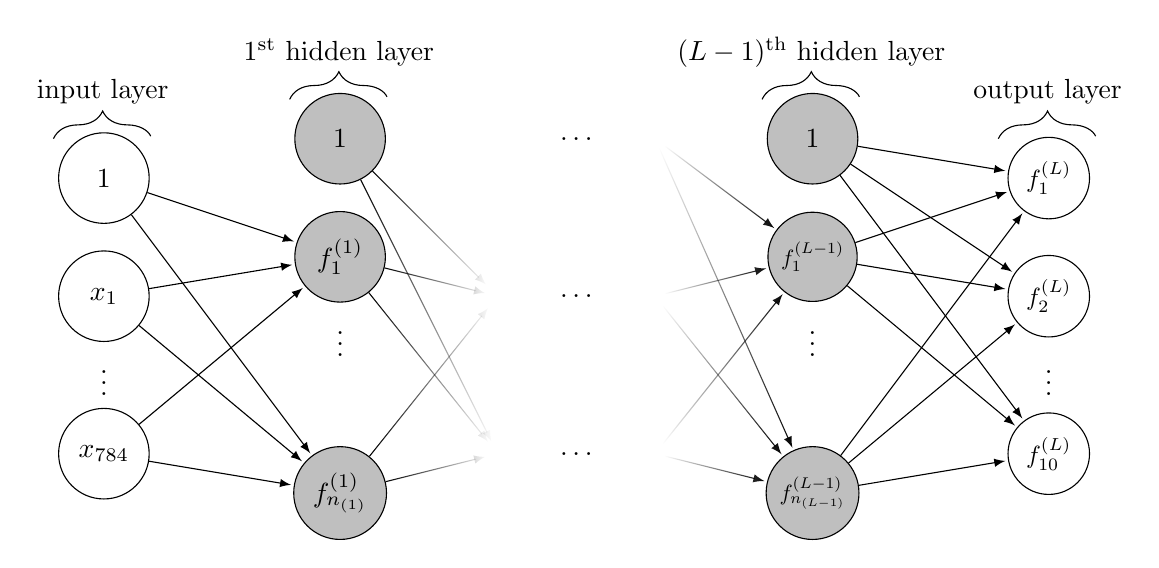
\begin{tikzpicture}[shorten >=1pt]
		\tikzstyle{unit}=[draw,shape=circle,minimum size=1.15cm]
		\tikzstyle{output}=[draw,shape=circle,minimum size=1.15cm,scale=0.9]
		\tikzstyle{hidden}=[draw,shape=circle,fill=black!25,minimum size=1.15cm]
 		\tikzstyle{lasthidden}=[draw,shape=circle,fill=black!25,minimum size=1.15cm,scale=0.8]

		\node[unit](x0) at (0,3.5){$1$};
		\node[unit](x1) at (0,2){$x_1$};
		\node at (0,1){\vdots};
		\node[unit](xd) at (0,0){$x_{784}$};
 
		\node[hidden](h10) at (3,4){$1$};
		\node[hidden](h11) at (3,2.5){$f_{1}^{(1)}$};
		\node at (3,1.5){\vdots};
		\node[hidden](h1m) at (3,-0.5){$f_{n_{(1)}}^{(1)}$};
 
		\node(h22) at (5,0){};
		\node(h21) at (5,2){};
		\node(h20) at (5,4){};
		
		\node(d3) at (6,0){$\ldots$};
		\node(d2) at (6,2){$\ldots$};
		\node(d1) at (6,4){$\ldots$};
 
		\node(hL12) at (7,0){};
		\node(hL11) at (7,2){};
		\node(hL10) at (7,4){};
		
		\node[hidden](hL0) at (9,4){$1$};
		\node[lasthidden](hL1) at (9,2.5){$f_1^{(L-1)}$};
		\node at (9,1.5){\vdots};
		\node[lasthidden](hLm) at (9,-0.5){$f_{n_{(L-1)}}^{(L-1)}$};
 
		\node[output](y1) at (12,3.5){$f_{1}^{(L)}$};
		\node[output](y2) at (12,2){$f_{2}^{(L)}$};
		\node at (12,1){\vdots};	
		\node[output](yc) at (12,0){$f_{10}^{(L)}$};
 
		\draw[->] (x0) -- (h11);
		\draw[->] (x0) -- (h1m);
 
		\draw[->] (x1) -- (h11);
		\draw[->] (x1) -- (h1m);
 
		\draw[->] (xd) -- (h11);
		\draw[->] (xd) -- (h1m);
 
		\draw[->] (hL0) -- (y1);
		\draw[->] (hL0) -- (yc);
		\draw[->] (hL0) -- (y2);
 
		\draw[->] (hL1) -- (y1);
		\draw[->] (hL1) -- (yc);
		\draw[->] (hL1) -- (y2);
 
		\draw[->] (hLm) -- (y1);
		\draw[->] (hLm) -- (y2);
		\draw[->] (hLm) -- (yc);
 
		\draw[->,path fading=east] (h10) -- (h21);
		\draw[->,path fading=east] (h10) -- (h22);
		
		\draw[->,path fading=east] (h11) -- (h21);
		\draw[->,path fading=east] (h11) -- (h22);
		
		\draw[->,path fading=east] (h1m) -- (h21);
		\draw[->,path fading=east] (h1m) -- (h22);
		
		\draw[->,path fading=west] (hL10) -- (hL1);
		\draw[->,path fading=west] (hL11) -- (hL1);
		\draw[->,path fading=west] (hL12) -- (hL1);
		
		\draw[->,path fading=west] (hL10) -- (hLm);
		\draw[->,path fading=west] (hL11) -- (hLm);
		\draw[->,path fading=west] (hL12) -- (hLm);
		
		\draw [decorate,decoration={brace,amplitude=10pt},xshift=-4pt,yshift=0pt] (-0.5,4) -- (0.75,4) node [black,midway,yshift=+0.6cm]{input layer};
		\draw [decorate,decoration={brace,amplitude=10pt},xshift=-4pt,yshift=0pt] (2.5,4.5) -- (3.75,4.5) node [black,midway,yshift=+0.6cm]{$1^{\text{st}}$ hidden layer};
		\draw [decorate,decoration={brace,amplitude=10pt},xshift=-4pt,yshift=0pt] (8.5,4.5) -- (9.75,4.5) node [black,midway,yshift=+0.6cm]{$(L-1)^{\text{th}}$ hidden layer};
		\draw [decorate,decoration={brace,amplitude=10pt},xshift=-4pt,yshift=0pt] (11.5,4) -- (12.75,4) node [black,midway,yshift=+0.6cm]{output layer};
	\end{tikzpicture}
	\caption[Network graph for a \textit{Fashion MNIST} classification.]{This figure illustrates a network graph for a \textit{Fashion MNIST} classification neural network. Output layer is fixed and uses \textit{softmax} activation function. Depending on experiment, other hidden layers vary in width and the activation function. More general implementation of this model is given in Figure \ref{fig:experiments:classification:model:nn-pytorch}.}
	\label{fig:experiments:classification:model:nn}
\end{figure}

\subsection{Methodology}
\label{section:experiments:classification:experiments-methodology}

Each experiment consists of a neural network architecture configuration and a training configuration. Experiments are run independently. 
Each experiment run consists of instantiation of a neural network from the configuration and training from scratch using training configuration from Table \ref{table:expriments:training_config}. In each experiment, the neural network architecture is fixed and only weights and biases are changed by the optimizer. After every 100 batch iterations, training and validation set accuracy and loss are computed for the experiment neural network architecture. The model achieving the best validation accuracy is maintained and its weights are saved. Plots in the subsequent sections were created by manual inspection and analysis of the following statistics:
\begin{itemize}[noitemsep]
    \item training and validation loss collected during the training process,
    \item training and validation accuracy collected during the training process,
    \item validation set accuracy and loss corresponding to the best weights,
    \item class-specific validation set accuracy corresponding to the best weights,
    \item confusion matrix corresponding to the model with the best weights.
\end{itemize}
\begin{figure}[H]
    \centering
    \begin{minted}[fontsize=\footnotesize]{python}
    layer_width = 64
    layers_number = 4
    layers = [ LayerConfig(layer_width, nn.ReLU()) for _ in range(layers_number) ]
    experiment = {
        'name' : 'nn-4x-64-relu-softmax',
        'epochs': 10,
        'batch_size' : 32,
        'layers_config': layers + [LayerConfig(10, nn.Softmax(dim=0))]
    }
    \end{minted}
    \caption{The configuration of \textit{nn-4x-64-relu-softmax} experiment}
    \label{fig:experiments:classification:experiment-example}
\end{figure}

\pagebreak
\subsection{The choice of an optimizer}
\label{subsection:experiments:classification:optimizer}
When it comes to optimizers, in this thesis we only discussed stochastic gradient descent. We briefly mentioned other methods of practical importance. However, the convergence of stochastic gradient descent was too slow under configuration from Table \ref{table:expriments:training_config} (see Table \ref{table:experiments:classification:optimizers-sigmoid} and Table \ref{table:experiments:classification:optimizers-relu}). 
Since the computational resources were limited, after experimenting with different optimizers, Adam produced the best results in the smallest number of training epochs. Adam is currently one of the most popular optimizers and it is a common default choice. The choice of an optimizer is a good example of a practical problem that is not discussed in the approximation theory of neural networks. Theoretical results are completely disconnected from choices regarding the optimization algorithm and its configuration. However, those may significantly affect the performance of the resulting neural network. Effects are especially noticeable when training for a fixed number of epochs, which is a very common practice. Given the fact an average training time of a network with a single hidden layer was about 30 minutes, the training time was indeed significantly affected. This observation was neatly summarised in \citetitle{ruder_2017_an} \cite{ruder_2017_an}, quoted below.

\begin{displayquote}[\citetitle{ruder_2017_an} \cite{ruder_2017_an}, p.10]
"Interestingly, many recent papers use vanilla SGD without momentum and a simple learning rate
annealing schedule. As has been shown, SGD usually achieves to find a minimum, but it might take
significantly longer than with some of the optimizers, is much more reliant on a robust initialization
and annealing schedule, and may get stuck in saddle points rather than local minima. Consequently,
if you care about fast convergence and train a deep or complex neural network, you should choose
one of the adaptive learning rate methods."
\end{displayquote}

The following results were obtained by changing the optimizer in configuration from Table \ref{table:expriments:training_config}. All optimizers were initialized with a default configuration.

\begin{table}[H]
    \centering
    \begin{tabular}{ | c | c | c | }
         \hline
         \textbf{model} & \textbf{SGD} & \textbf{Adam} \\
         \hline
         nn-16-sigmoid-softmax & 70.9800\% & 79.2200\% \\
         \hline
         nn-32-sigmoid-softmax & 70.8300\% & 79.8700\% \\
         \hline
         nn-64-sigmoid-softmax & 70.1500\% & 79.0100\% \\
         \hline
         nn-128-sigmoid-softmax & 68.6500\% & 79.4500\% \\
         \hline
    \end{tabular}

    \caption{validation set accuracy of sigmoid networks after 5 training epochs}
    \label{table:experiments:classification:optimizers-sigmoid}
\end{table}
\begin{table}[H]
    \centering
    \begin{tabular}{ | c | c | c | }
         \hline
         \textbf{model} & \textbf{SGD} & \textbf{Adam} \\
         \hline
         nn-16-relu-softmax & 72.5100\% & 76.7800\% \\
         \hline
         nn-32-relu-softmax & 72.5400\% & 76.6100\% \\
         \hline
         nn-64-relu-softmax & 72.8500\% & 77.2100\% \\
         \hline
         nn-128-relu-softmax & 72.8900\% & 77.4200\% \\
         \hline
    \end{tabular}

    \caption{validation set accuracy of ReLU networks after 5 training epochs}
    \label{table:experiments:classification:optimizers-relu}
\end{table}
\subsection{Impact of batch size on validation accuracy}
\label{subsection:experiments:classification:batch}
Although the batch size seems unimportant in comparison with neural network architecture and the choice of an optimizer, the experimental data from Figure \ref{figure:experiments:classification:batch-size-plot} indicates that the batch size plays an important role when the network is trained for a fixed number of iterations. To examine the effects of various batch sizes, a reasonably large neural network architecture is chosen and such a network is trained using the configuration from Table \ref{table:expriments:training_config}. In this experiment, only the batch size and activation function are varied. It is very important to note that the number of epochs remained unchanged. 

The results displayed in Figure \ref{figure:experiments:classification:batch-size-plot} indicate that training using smaller batch sizes results in significantly greater validation accuracy. This can be attributed to the fact that a smaller batch size implies a greater number of parameter updates since the number of epochs is fixed. It is worth noting that such a training setup requires significantly more time. For instance, the average training time using a batch size of 32 examples was about 30 minutes, while the average training time using the batch size of 256 examples was about 5 minutes. The accuracy drop after the batch size of 128 is noticeable for every activation function. This could be expected since the number of parameter updates drops significantly. On the other hand, a larger batch size often results in a more accurate estimate of the gradient.

It seems that larger batch sizes generally require a larger number of training epochs, which is indeed sensible, as the optimization performs significantly less parameter updates. It is reasonable to conjecture that the sweet spot for the default training configuration is a batch size of 64 examples, as it seems that such a configuration performs slightly better than other batch sizes in 2 out of 3 activation functions.

To sum up, batch size likely plays an important role in training a neural network. The results discussed are relevant only for one neural network architecture and one default training setup. However, according to the Figure 1 from \cite{hoffer_2018_train} and Figure 2 from \cite{shirishkeskar_2017_on}, the similar observations can be made on more complex datasets and neural networks. It is interesting to note that \cite{hoffer_2018_train} and \cite{shirishkeskar_2017_on} provide different explanations and analysis of this phenomenon.

\begin{figure}[H]
    \centering
    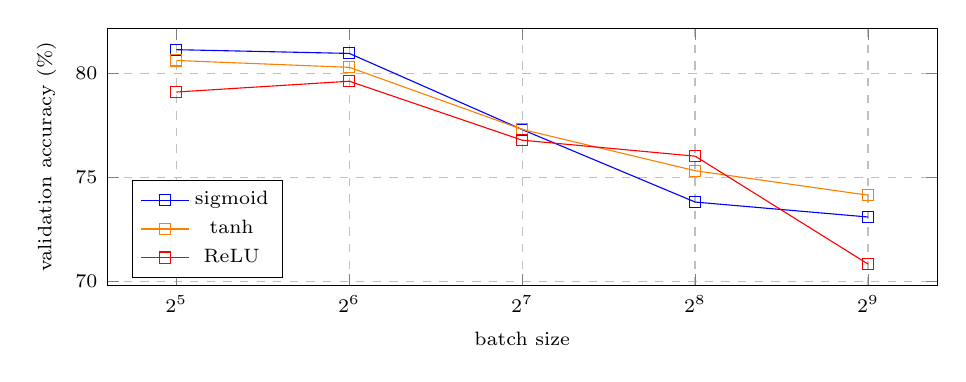
\begin{tikzpicture}
        \begin{axis}[
            height=0.4\textwidth,
            width=\textwidth,
            xlabel={batch size},
            ylabel={validation accuracy (\%)},
            ymajorgrids=true,
            grid style=dashed,
            xmode=log,
            legend pos=south west,
            log basis x={2}]
            \addplot[mark=square,blue] coordinates {(32,81.15) (64,80.97) (128,77.30) (256,73.81) (512,73.09)};
            \addplot[mark=square,orange] coordinates {(32,80.63) (64,80.30) (128,77.31) (256,75.32) (512,74.14)};
            \addplot[mark=square,red] coordinates {(32,79.11) (64,79.63) (128,76.79) (256,76.02) (512,70.82)};
            \legend{sigmoid, tanh, ReLU}
        \end{axis}
    \end{tikzpicture}
    \caption{Effects of various batch sizes on training \textit{nn-2x-128-sigmoid-softmax}}
    \label{figure:experiments:classification:batch-size-plot}
\end{figure}
\subsection{Impact of activation function on validation accuracy}
\label{subsection:experiments:classification:activation}
Since the activation function gives rise to nonlinearity, it is reasonable to conjecture that the activation function affects performance. In \nameref{chapter:literature-review} and \nameref{chapter:universality}, we have also observed that the properties of activation function also play an essential role in many proofs of universality.

To begin an experimental study of the effects of the activation function, we will focus on neural networks with a single hidden layer. Each neural network is trained using the configuration from Table \ref{table:expriments:training_config}. In this experiment, only the hidden layer width and the activation function are varied. For each experiment configuration, the model achieving the best validation accuracy is saved and used in the following analysis.

According to the results displayed in Figure \ref{fig:experiments:classification:all-activations-plot}, it is likely that the activation function significantly affects validation set accuracy, given current training configuration. Thus, it is reasonable to conjecture that the activation function affects the generalization error. It is interesting to note that sigmoid and $\tanh$ significantly and consistently outperform $\operatorname{ReLU}$ regardless of hidden layer width. That is slightly surprising because many modern neural network architectures use $\operatorname{ReLU}$ and similar rectified activation functions instead of $\operatorname{sigmoid}$ and $\tanh$.

It can be shown that $\operatorname{sigmoid}$  and $\tanh$ are algebraically related. More precisely, for every $x \in \R, \tanh{(x)} = 2\sigma(2x) - 1$. Given the structure of a fully-connected neural network and this algebraic connection, it is reasonable to expect that $\operatorname{sigmoid}$  and $\tanh$ produce similar results. According to the results displayed in Figure \ref{fig:experiments:classification:all-activations-plot}, that is indeed the case. Another surprising observation is the significant validation accuracy drop for $\operatorname{ReLU}$ networks after hidden layer width of 128 neurons. Although ReLU networks perform worse as the hidden layer width increases, it seems that $\operatorname{sigmoid}$ and $\tanh$ networks perform better. The widest $\tanh$ and $\operatorname{sigmoid}$ achieve the best validation accuracy. We will briefly discuss the worst $\operatorname{ReLU}$ model. According to the Figure \ref{fig:experiments:classification:wide-relu-plot}, validation and test accuracy are consistently very similar. Hence, there is no evidence of overfitting.

\begin{figure}[H]
    \begin{minipage}{.5\textwidth}
        \centering
        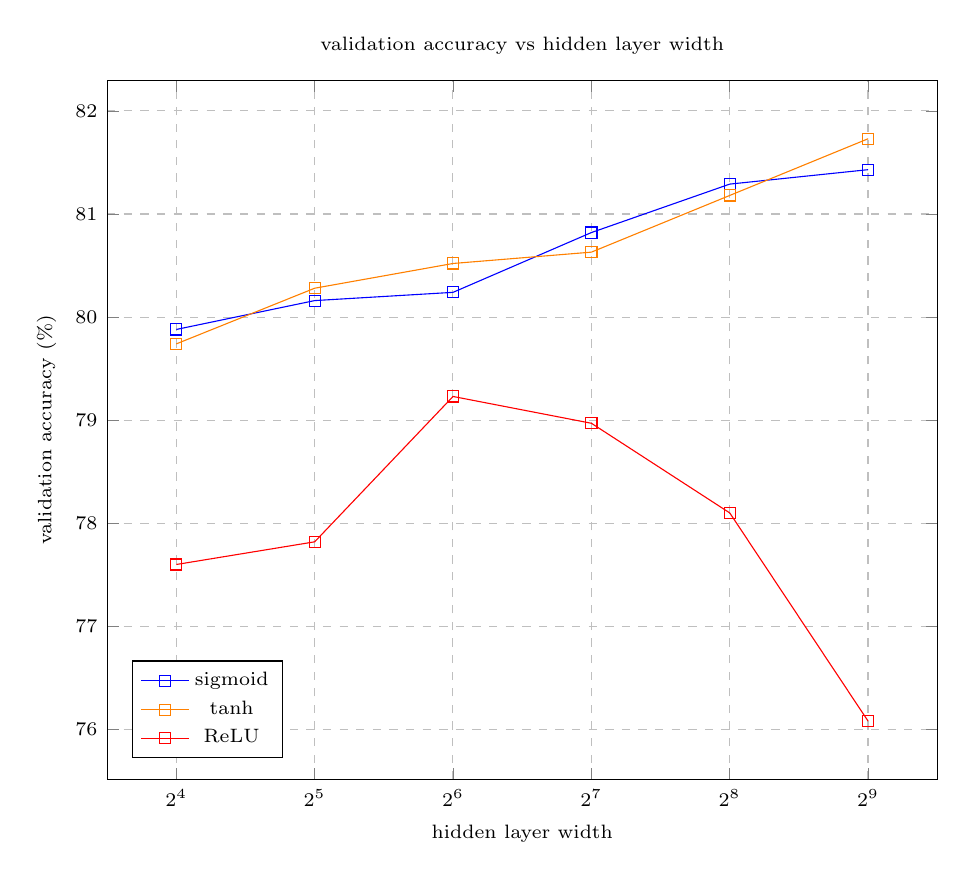
\begin{tikzpicture}
            \begin{axis}[
                width=\textwidth,
                title={validation accuracy vs hidden layer width},
                xlabel={hidden layer width},
                ylabel={validation accuracy (\%)},
                ymajorgrids=true,
                grid style=dashed,
                xmode=log,
                legend pos=south west,
                log basis x={2}]
                \addplot[mark=square,blue] coordinates {(16,79.88) (32,80.16) (64,80.24) (128,80.82) (256,81.29) (512,81.43)};
                \addplot[mark=square,orange] coordinates {(16,79.74) (32,80.28) (64,80.52) (128,80.63) (256,81.18) (512,81.73)};
                \addplot[mark=square,red] coordinates {(16,77.60) (32,77.82) (64,79.23) (128,78.97) (256,78.10) (512,76.08)};
                \legend{sigmoid, tanh, ReLU}
            \end{axis}
        \end{tikzpicture}
        \captionof{figure}{Validation accuracy of the best model with given hidden layer width and activation function}
        \label{fig:experiments:classification:all-activations-plot}
    \end{minipage}%
    \hspace{0.5cm}
    \begin{minipage}{.5\textwidth}
        \centering
        \includegraphics[scale=0.5]{experiments/classification/relu-single-layer-no-overfitting.png}
        \captionof{figure}{Training and validation accuracy of $\operatorname{ReLU}$ network with a single hidden layer of 512 neurons. This is the worst $\operatorname{ReLU}$ model in this experiment.}
        \label{fig:experiments:classification:wide-relu-plot}
    \end{minipage}
\end{figure}


\subsection{Adding a layer}
\label{subsection:experiments:classification:adding-a-layer}
In this subsection, we will focus on neural networks with two hidden layers of the same width. The experiment configuration is almost identical to one from the previous section. The only change is the addition of another identical hidden layer to each neural network.
For each experiment configuration, the model achieving the best validation accuracy is saved and used in the following analysis.

From Figure \ref{fig:experiments:classification:all-activations-plot}, it is noticeable that the best validation accuracy increases consistently with the hidden layer width. This may suggest that $\operatorname{sigmoid}$ and $\operatorname{tanh}$ neural networks may benefit from the increased model complexity. However, it seems that this does not happen to the extent one may expect (see Figure \ref{fig:experiments:classification:adding-a-layer-all-activations}).

In the previous section, we discussed the similarity between the $\operatorname{sigmoid}$ and $\operatorname{tanh}$ activation function. From the Figure \ref{fig:experiments:classification:adding-a-layer-all-activations}, we can conclude that $\operatorname{sigmoid}$ and $\operatorname{tanh}$ networks remain achieving similar validation accuracy, what is compatible with results from the previous section.

From Figure \ref{fig:experiments:classification:adding-a-layer-sigmoid}, Figure \ref{fig:experiments:classification:adding-a-layer-tanh} and Figure \ref{fig:experiments:classification:adding-a-layer-relu}, it is evident that the layer addition results in slightly better validation accuracy for layer widths up to and including 128 neurons. However, the difference is mostly within $1.5\%$ and this can be attributed to the noise. It is hard to say whether the validation accuracy boost is significant. According to the benchmark table in \cite{fashionmnistgithub}, similar neural networks may achieve the validation accuracy of $88\%$ (see the entry for \textit{MLP 256-128-100}). The pattern is slightly unclear for layer widths larger than 128 neurons. For instance, the network with $\operatorname{tanh}$ activation and two hidden layers of 512 neurons achieved the validation accuracy of $82.33\%$, which is the best validation accuracy so far. However, such a configuration performed noticeably less well for other activation functions, especially $\operatorname{ReLU}$.

Neural networks with $\operatorname{tanh}$ activation function benefited the most from the extra layer. According to Figure \ref{fig:experiments:classification:adding-a-layer-tanh}, $\operatorname{tanh}$ neural networks with two identical layers consistently performed at least as well as the corresponding single layer configuration. It is interesting to note that $\operatorname{ReLU}$ networks benefited the least from the extra layer. This observation is quite evident from the Figure \ref{fig:experiments:classification:adding-a-layer-relu}. As in the case of neural networks with the single layer, $\operatorname{ReLU}$ networks seem to generalize slightly worse than $\operatorname{tanh}$ and $\operatorname{sigmoid}$ networks.

\begin{figure}[H]
    \centering
    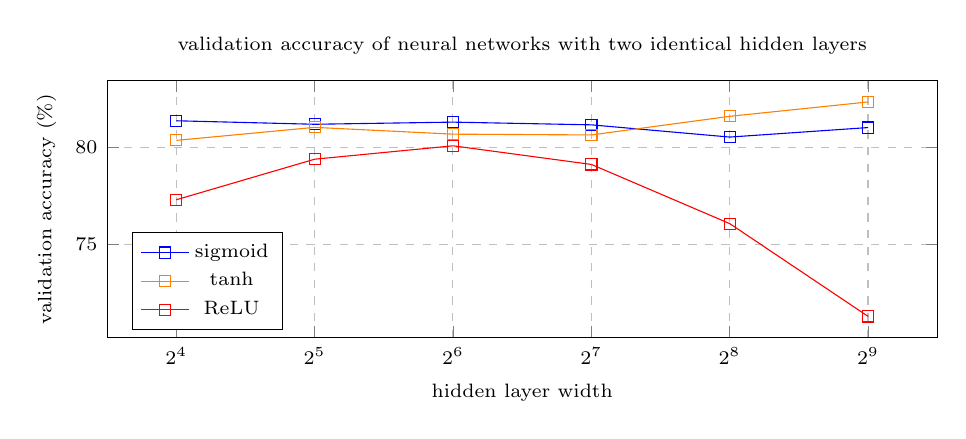
\begin{tikzpicture}
        \begin{axis}[
            height=0.4\textwidth,
            title={validation accuracy of neural networks with two identical hidden layers},
            width=\textwidth,
            xlabel={hidden layer width},
            ylabel={validation accuracy (\%)},
            ymajorgrids=true,
            grid style=dashed,
            xmode=log,
            legend pos=south west,
            log basis x={2}]
            \addplot[mark=square,blue] coordinates {(16,81.36) (32,81.18) (64, 81.29) (128,81.15) (256,80.52) (512,81.01)};
            \addplot[mark=square,orange] coordinates {(16,80.35) (32,81.02) (64,80.67) (128,80.63) (256,81.59) (512,82.33)};
            \addplot[mark=square,red] coordinates {(16,77.29) (32,79.38) (64,80.07) (128,79.11) (256,76.06) (512,71.28)};
            \legend{sigmoid, tanh, ReLU}
        \end{axis}
    \end{tikzpicture}
    \caption{Validation accuracy for networks with two identical hidden layers}
    \label{fig:experiments:classification:adding-a-layer-all-activations}
\end{figure}
\newpage
\begin{figure}[H]
    \centering
    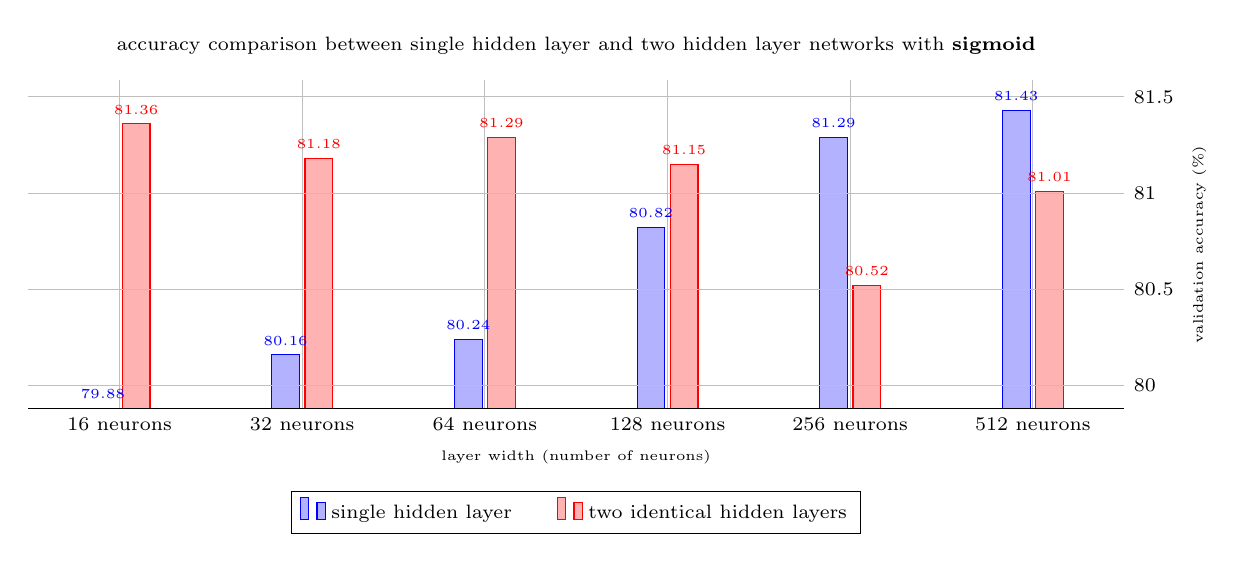
\begin{tikzpicture}
      \centering
      \begin{axis}[
            ybar, axis on top,
            title={accuracy comparison between single hidden layer and two hidden layer networks with \textbf{sigmoid}},
            height=5.75cm, width=15.5cm,
            tick align=inside,
            enlarge y limits={value=.1,upper},
            axis x line*=bottom,
            axis y line*=right,
            y axis line style={opacity=0},
            tickwidth=0pt,
            enlarge x limits=true,
            legend style={
                at={(0.5,-0.25)},
                anchor=north,
                legend columns=-1,
                /tikz/every even column/.append style={column sep=0.5cm}
           },
           ylabel={validation accuracy (\%)},
           symbolic x coords={
               16 neurons, 32 neurons, 64 neurons, 128 neurons,
               256 neurons, 512 neurons
           },
           xtick=data,
           xlabel={layer width (number of neurons)},
           label style={font=\tiny},
           every node near coord/.append style={font=\tiny},
           nodes near coords={
            \pgfmathprintnumber[precision=2]{\pgfplotspointmeta}
           }
        ]
        \addplot coordinates {
            (16 neurons,79.88) 
            (32 neurons,80.16) 
            (64 neurons,80.24) 
            (128 neurons,80.82) 
            (256 neurons,81.29) 
            (512 neurons,81.43)
        };
        \addplot coordinates {
            (16 neurons,81.36) 
            (32 neurons,81.18) 
            (64 neurons, 81.29) 
            (128 neurons,81.15) 
            (256 neurons,80.52) 
            (512 neurons,81.01)
        };
        \legend{single hidden layer, two identical hidden layers}
      \end{axis}
    \end{tikzpicture}
    \caption{Validation accuracy for \textbf{sigmoid}  grouped by number of layers}
    \label{fig:experiments:classification:adding-a-layer-sigmoid}
\end{figure}
\begin{figure}[H]
    \centering
    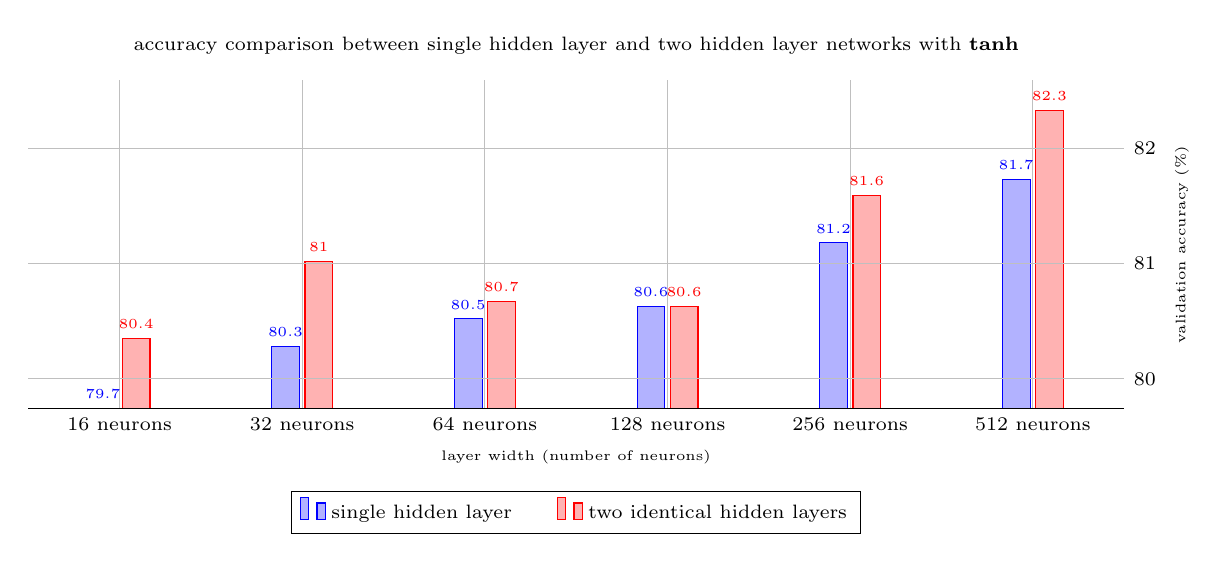
\begin{tikzpicture}
      \centering
      \begin{axis}[
            ybar, axis on top,
            title={accuracy comparison between single hidden layer and two hidden layer networks with \textbf{tanh}},
            height=5.75cm, width=15.5cm,
            tick align=inside,
            enlarge y limits={value=.1,upper},
            axis x line*=bottom,
            axis y line*=right,
            y axis line style={opacity=0},
            tickwidth=0pt,
            enlarge x limits=true,
            legend style={
                at={(0.5,-0.25)},
                anchor=north,
                legend columns=-1,
                /tikz/every even column/.append style={column sep=0.5cm}
           },
           ylabel={validation accuracy (\%)},
            symbolic x coords={
               16 neurons, 32 neurons, 64 neurons, 128 neurons,
               256 neurons, 512 neurons
            },
           xtick=data,
           xlabel={layer width (number of neurons)},
           label style={font=\tiny},
           every node near coord/.append style={font=\tiny},
           nodes near coords={
            \pgfmathprintnumber[precision=1]{\pgfplotspointmeta}
           }
        ]
        
        \addplot coordinates {
            (16 neurons,79.74) 
            (32 neurons,80.28) 
            (64 neurons,80.52) 
            (128 neurons,80.63) 
            (256 neurons,81.18) 
            (512 neurons,81.73)
        };
        \addplot coordinates {
            (16 neurons,80.35) 
            (32 neurons,81.02) 
            (64 neurons,80.67) 
            (128 neurons,80.63) 
            (256 neurons,81.59) 
            (512 neurons,82.33)
        };
        \legend{single hidden layer, two identical hidden layers}
      \end{axis}
    \end{tikzpicture}  
    \caption{Validation accuracy for \textbf{tanh} grouped by the number of layers}
    \label{fig:experiments:classification:adding-a-layer-tanh}
\end{figure}
\begin{figure}[H]
    \centering
    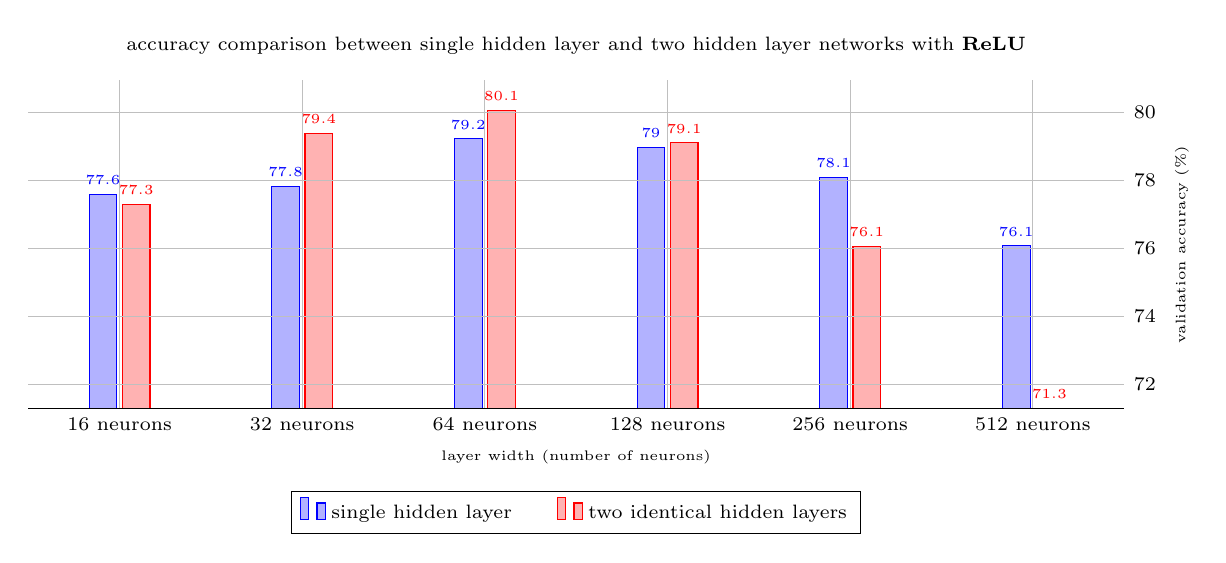
\begin{tikzpicture}
      \centering
      \begin{axis}[
            ybar, axis on top,
            title={accuracy comparison between single hidden layer and two hidden layer networks with \textbf{ReLU}},
            height=5.75cm, width=15.5cm,
            tick align=inside,
            enlarge y limits={value=.1,upper},
            axis x line*=bottom,
            axis y line*=right,
            y axis line style={opacity=0},
            tickwidth=0pt,
            enlarge x limits=true,
            legend style={
                at={(0.5,-0.25)},
                anchor=north,
                legend columns=-1,
                /tikz/every even column/.append style={column sep=0.5cm}
           },
           ylabel={validation accuracy (\%)},
            symbolic x coords={
               16 neurons, 32 neurons, 64 neurons, 128 neurons,
               256 neurons, 512 neurons
            },
           xtick=data,
           label style={font=\tiny},
           xlabel={layer width (number of neurons)},
           every node near coord/.append style={font=\tiny},
           nodes near coords={
            \pgfmathprintnumber[precision=1]{\pgfplotspointmeta}
           }
        ]
        \addplot coordinates {
            (16 neurons,77.60)
            (32 neurons,77.82) 
            (64 neurons,79.23) 
            (128 neurons,78.97) 
            (256 neurons,78.10) 
            (512 neurons,76.08)
        };
        \addplot coordinates {
            (16 neurons,77.29) 
            (32 neurons,79.38) 
            (64 neurons,80.07) 
            (128 neurons,79.11) 
            (256 neurons,76.06) 
            (512 neurons,71.28)
        };
        \legend{single hidden layer, two identical hidden layers}
      \end{axis}
    \end{tikzpicture}  
    \caption{Validation accuracy for \textbf{ReLU} grouped by the number of layers}
    \label{fig:experiments:classification:adding-a-layer-relu}
\end{figure}
\subsection{Impact of neural network depth on validation accuracy}
\label{subsection:experiments:classification:depth}
In this subsection, we will discuss the relationship between the best validation accuracy and neural network depth. The experiment setup and methodology are almost identical to the previous subsection. The only change is the addition of multiple identical hidden layers instead of a single hidden layer.
In the previous subsection, we observed that the addition of a single identical layer did not significantly improve the validation accuracy. According to the results presented in Figure \ref{figure:experiments:classification:depth:64} and in Figure \ref{figure:experiments:classification:depth:128}, validation accuracy does not improve with addition of identically wide hidden layers. Hence, we may conjecture that on this dataset, deeper fully-connected networks do not generalize better than shallow fully-connected networks. It is important to note that results are consistent across all activation functions. 
Moreover, results in Figure \ref{figure:experiments:classification:depth:64} and Figure \ref{figure:experiments:classification:depth:128} are almost identical. This can be attributed to the apparent similarity in neural network architecture.

It is interesting to note that the validation accuracy remains close to $80 \%$ for networks with at most 4 layers. However, as the number of layers increases, the validation accuracy significantly decreases. This observation applies to all activation functions. However the validation accuracy drop is the largest for $\operatorname{sigmoid}$ and $\tanh$. This can be attributed to a well-known \textit{vanishing gradient} problem. We will briefly discuss that source of difficulty in training deep neural networks with $\operatorname{sigmoid}$ activation. We know that $\lim_{x \to \infty} \sigma (x) = 1$ and $\lim_{x \to -\infty} \sigma (x) = 0$. By Lemma \ref{lemma:introduction:activation:sigmoid-derivative}, we conclude that $\lim_{x \to \infty} \sigma'(x) = 0$ and $\lim_{x \to -\infty} \sigma'(x) = 0$. Informally, as the inputs of a $\operatorname{sigmoid}$ layer become extremely small or extremely large, the gradient of the loss function with respect to parameters of a $\operatorname{sigmoid}$ layer vanishes. This causes serious problems in gradient-based optimization since the corresponding weights and biases cease to update. However, in case of $\operatorname{ReLU}$, the drop in validation accuracy resulting from increased depth is noticeably smaller than in case of $\operatorname{sigmoid}$ and $\tanh$. This is also a known result and one of key reasons why $\operatorname{ReLU}$ is preferred to $\operatorname{sigmoid}$ and $\tanh$ when training deep networks.

\begin{figure}[H]
    \centering
    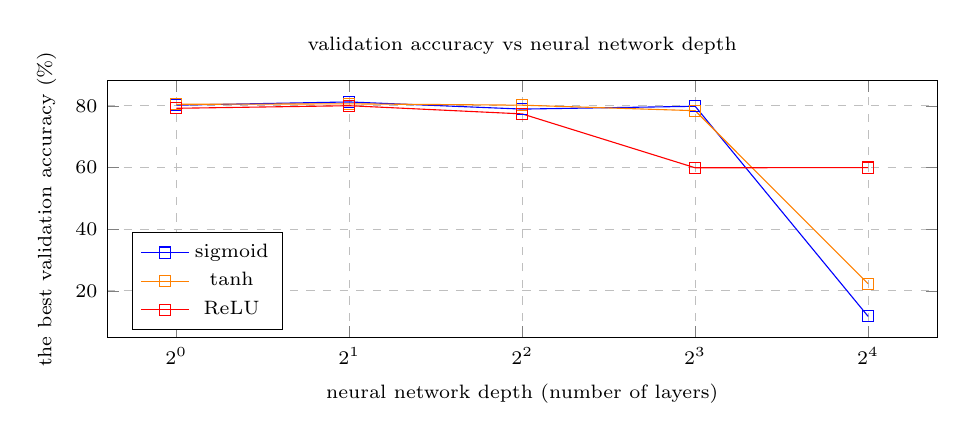
\begin{tikzpicture}
        \begin{axis}[
            height=0.4\textwidth,
            width=\textwidth,
            title= {validation accuracy vs neural network depth},
            xlabel={neural network depth (number of layers)},
            ylabel={the best validation accuracy (\%)},
            ymajorgrids=true,
            grid style=dashed,
            xmode=log,
            legend pos=south west,
            log basis x={2}]
            \addplot[mark=square,blue] coordinates {(1,80.24) (2,81.29) (4, 78.97) (8,79.88) (16,11.72)};
            \addplot[mark=square,orange] coordinates {(1,80.52) (2,80.67) (4,80.24) (8,78.45) (16,22.30)};
            \addplot[mark=square,red] coordinates {(1,79.23) (2,80.07) (4,77.41) (8,59.93) (16,60.00)};
            \legend{sigmoid, tanh, ReLU}
        \end{axis}
    \end{tikzpicture}
    \caption{Effects of varying neural network depth while keeping layer width of \textbf{64 neurons}}
    \label{figure:experiments:classification:depth:64}
\end{figure}
\begin{figure}[H]
    \centering
    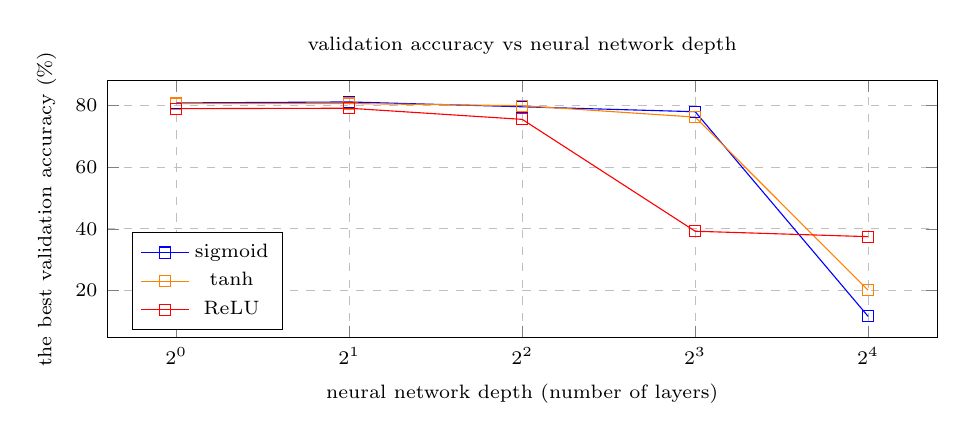
\begin{tikzpicture}
        \begin{axis}[
            height=0.4\textwidth,
            width=\textwidth,
            title= {validation accuracy vs neural network depth},
            xlabel={neural network depth (number of layers)},
            ylabel={the best validation accuracy  (\%)},
            ymajorgrids=true,
            grid style=dashed,
            xmode=log,
            legend pos=south west,
            log basis x={2}]
            \addplot[mark=square,blue] coordinates {(1,80.82) (2,81.15) (4, 79.58) (8,77.98) (16,11.60)};
            \addplot[mark=square,orange] coordinates {(1,80.63) (2,80.63) (4,79.93) (8,76.24) (16,20.05)};
            \addplot[mark=square,red] coordinates {(1,78.97) (2,79.11) (4,75.50) (8,39.22) (16,37.46)};
            \legend{sigmoid, tanh, ReLU}
        \end{axis}
    \end{tikzpicture}
    \caption{Effects of varying neural network depth while keeping layer width of \textbf{128 neurons}}
    \label{figure:experiments:classification:depth:128}
\end{figure}
\subsection{Interesting observation}

According to Figure \ref{figure:experiments:classification:accuracy-per-class-best}, two  models achieving the best validation accuracy, \textit{nn-2x-512-tanh-softmax} and \textit{nn-512-sigmoid-softmax}, demonstrate similar performance on every label.
However, it is interesting to observe that both models struggle with \textit{shirt}s. Although both models perform decently on \textit{pullover} and \textit{T-shirt}, they both perform significantly worse on \textit{shirt}. 

Figure \ref{fig:experiments:classification:best-tanh} demonstrates that the training and accuracy gap of \textit{nn-2x-512-tanh-softmax} remains quite small. However, in Figure \ref{fig:experiments:classification:best-sigmoid}, we can observe slightly larger gap between training and validation accuracy of \textit{nn-512-sigmoid-softmax}. Since the training accuracy of both models peaks at about $82 \%$, there is evidence to suggest both models struggle to fit the training set. Hence, there is no evidence that those networks overfit. In the previous section, we observed that the addition of more fully-connected layers does not significantly affect the generalization. This may indicate that fully-connected architecture is generally too simple for this dataset.


\begin{figure}[H]
    \centering
    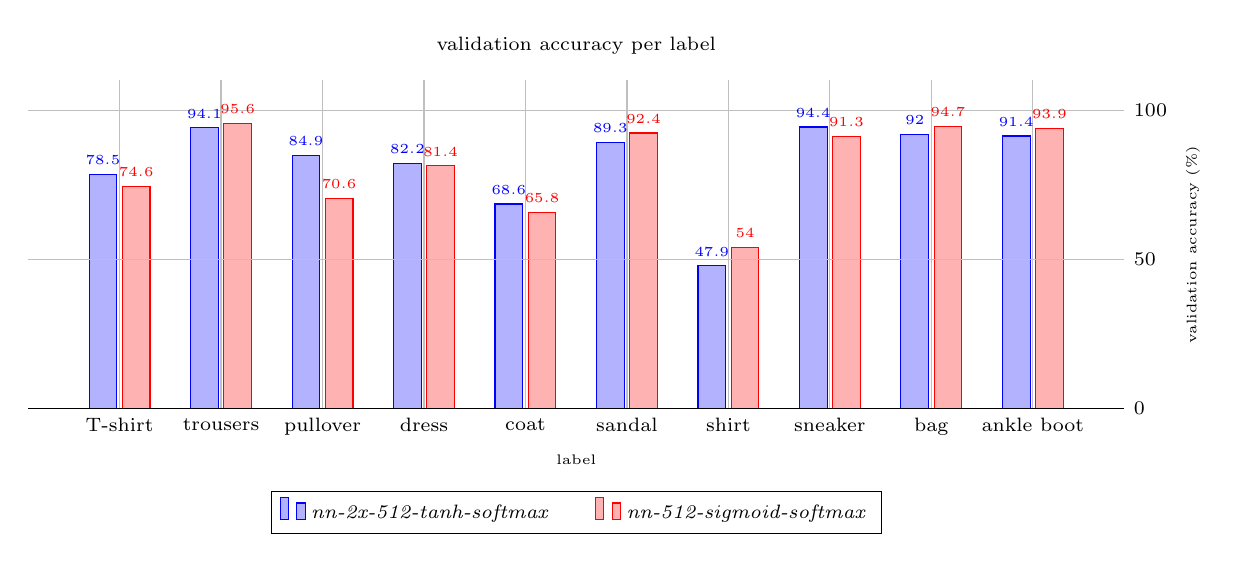
\begin{tikzpicture}
        \begin{axis}[
            symbolic x coords={T-shirt,trousers,pullover,dress,coat,sandal,shirt,sneaker,bag,ankle boot},
            width=15.5cm,
            height=5.75cm,
            ymax=100,
            ymin=0,
            xtick=data,
            ybar, axis on top,
            title={validation accuracy per label},
            height=5.75cm, width=15.5cm,
            tick align=inside,
            enlarge y limits={value=.1,upper},
            axis x line*=bottom,
            axis y line*=right,
            y axis line style={opacity=0},
            tickwidth=0pt,
            enlarge x limits=true,
            legend style={
                at={(0.5,-0.25)},
                anchor=north,
                legend columns=-1,
                /tikz/every even column/.append style={column sep=0.5cm}
           },
           ylabel={validation accuracy (\%)},
           xtick=data,
           xlabel={label},
           label style={font=\tiny},
           every node near coord/.append style={font=\tiny},
           nodes near coords={
            \pgfmathprintnumber[precision=2]{\pgfplotspointmeta}
           }
        ]
            \addplot coordinates {
                (T-shirt, 78.50)
                (trousers, 94.10)
                (pullover, 84.90)
                (dress, 82.20)
                (coat, 68.60)
                (sandal, 89.30)
                (shirt, 47.90)
                (sneaker, 94.40)
                (bag, 92.00)
                (ankle boot, 91.40)
            };
            \addplot coordinates {
                (T-shirt, 74.60)
                (trousers, 95.60)
                (pullover, 70.60)
                (dress, 81.40)
                (coat, 65.80)
                (sandal, 92.40)
                (shirt, 54.00)
                (sneaker, 91.30)
                (bag, 94.70)
                (ankle boot, 93.90)
            };
            \legend{\textit{nn-2x-512-tanh-softmax},\textit{nn-512-sigmoid-softmax}}
        \end{axis}

    \end{tikzpicture}
    \caption{Validation accuracy per label for the best network configurations}
    \label{figure:experiments:classification:accuracy-per-class-best}
\end{figure}
\begin{figure}[H]
    \begin{minipage}{.5\textwidth}
        \centering
        \includegraphics[scale=0.5]{experiments/classification/tanh.png}
        \captionof{figure}{Accuracy pattern of \textit{nn-2x-512-tanh-softmax} }
        \label{fig:experiments:classification:best-tanh}
    \end{minipage}%
    \hspace{0.25cm}
    \begin{minipage}{.5\textwidth}
        \centering
        \includegraphics[scale=0.5]{experiments/classification/sigmoid.png}
        \captionof{figure}{Accuracy pattern of \textit{nn-512-sigmoid-softmax}}
        \label{fig:experiments:classification:best-sigmoid}
    \end{minipage}
\end{figure}

\subsection{Conclusion}

In this chapter, we discussed various practical problems related to the applications of neural networks. Despite impressive theoretical properties discussed in \nameref{chapter:literature-review} and \nameref{chapter:universality}, many practical applications of neural networks often suffer from issues not addressed in the universal approximation theory. 

According to state of the art results from  \nameref{chapter:literature-review}, $\operatorname{ReLU}$, $\operatorname{sigmoid}$ and $\operatorname{tanh}$ have comparable theoretical properties. However, in \nameref{subsection:experiments:classification:activation}, we observed that those activation functions result in noticeably different validation accuracy. This can be attributed to the little emphasis we put on the training configuration. This suggests that different activation functions may demand different training configurations. To address a mysterious performance gap between $\operatorname{ReLU}$ and alternatives,
more research is necessary. For example, studying the effects of weight regularisation (weight decay) or employing a more flexible learning rate scheduler could provide more insight into this observation. According to the results reported on the  \href{http://fashion-mnist.s3-website.eu-central-1.amazonaws.com/}{Fashion MNIST benchmark dashboard}, a neural network with a single layer of 100 neurons and $\operatorname{ReLU}$ activation function achieved the accuracy of $87.7\%$. Moreover, such a network outperformed $\tanh$ counterparts. This may suggest that $\operatorname{ReLU}$ networks perform better than observed in this thesis.

We have also observed that the best validation accuracy peaks at about $82\%$.  According to the benchmark table in \cite{fashionmnistgithub}, more sophisticated convolutional neural networks achieve the validation accuracy exceeding $90\%$. This may indicate that the fully-connected architecture is generally too simple to perform the classification on this dataset.

Seemingly unimportant hyperparameter choices discussed in \nameref{subsection:experiments:classification:batch} and \nameref{subsection:experiments:classification:optimizer} are disconnected from the approximation theory of neural networks. However, we observed they may have significant practical consequences.
\subsection{Conclusion}

In this chapter, we discussed various practical problems related to the applications of neural networks. Despite impressive theoretical properties discussed in \nameref{chapter:literature-review} and \nameref{chapter:universality}, many practical applications of neural networks often suffer from issues not addressed in the universal approximation theory. 

According to state of the art results from  \nameref{chapter:literature-review}, $\operatorname{ReLU}$, $\operatorname{sigmoid}$ and $\operatorname{tanh}$ have comparable theoretical properties. However, in \nameref{subsection:experiments:classification:activation}, we observed that those activation functions result in noticeably different validation accuracy. This can be attributed to the little emphasis we put on the training configuration. This suggests that different activation functions may demand different training configurations. To address a mysterious performance gap between $\operatorname{ReLU}$ and alternatives,
more research is necessary. For example, studying the effects of weight regularisation (weight decay) or employing a more flexible learning rate scheduler could provide more insight into this observation. According to the results reported on the  \href{http://fashion-mnist.s3-website.eu-central-1.amazonaws.com/}{Fashion MNIST benchmark dashboard}, a neural network with a single layer of 100 neurons and $\operatorname{ReLU}$ activation function achieved the accuracy of $87.7\%$. Moreover, such a network outperformed $\tanh$ counterparts. This may suggest that $\operatorname{ReLU}$ networks perform better than observed in this thesis.

We have also observed that the best validation accuracy peaks at about $82\%$.  According to the benchmark table in \cite{fashionmnistgithub}, more sophisticated convolutional neural networks achieve the validation accuracy exceeding $90\%$. This may indicate that the fully-connected architecture is generally too simple to perform the classification on this dataset.

Seemingly unimportant hyperparameter choices discussed in \nameref{subsection:experiments:classification:batch} and \nameref{subsection:experiments:classification:optimizer} are disconnected from the approximation theory of neural networks. However, we observed they may have significant practical consequences.

\chapter{Appendix}
\label{chapter:appendix}
This chapter is devoted mainly to the mathematics backing the main results established in \nameref{chapter:universality}.
Although many results discussed in this chapter are standard results in their respective fields, most of them are often not part of the undergraduate syllabus. The results that were part of the syllabus will be referenced. The most important results that were not part of the syllabus will be stated and proved.
This chapter also contains the \nameref{section:appendix:code} and \nameref{section:appendix:statement}.
\section{Set Theory}

The only axiomatic set-theoretic result relevant to this work is \nameref{lemma:set:zorn}.
To state the \nameref{lemma:set:zorn}, we recall various ordering concepts.

\begin{definition}[partial order]
\label{defn:set:porder}
Suppose that $\Omega$ is a nonempty set and $\prec$ is a binary relation on $\Omega$. We say
$\prec$ is a partial order if:
\begin{axioms}{P}
  \item \label{defn:set:porder:P1} $x \prec x$ for every $x \in \Omega$;
  \item \label{defn:set:porder:P2} if $x \prec y$ and $y \prec x$ then $x = y$;
  \item \label{defn:set:porder:P3} if $x \prec y$ and $y \prec z$ then $x \prec z$.
\end{axioms}
If $\prec$ is a partial order, we say $\Omega$ is a partially ordered set.
\end{definition}
\begin{definition}[total order]
\label{defn:set:torder}
Suppose that $\Omega$ is a nonempty set and $\prec$ is a partial order on $\Omega$.
If for every $x, y \in \Omega$ either $x \prec y$ or $y \prec x$, we say that $\prec$ is a total order and we say $\Omega$ is a totally ordered set.
\end{definition}
\begin{definition}[maximal element]
\label{defn:set:maxelem}
Suppose that $\Omega$ is a nonempty set and $\prec$ is a partial order on $\Omega$.
Then $y \in \Omega$ is a maximal element of $\Omega$ if $y \prec x \implies y = x$.
\end{definition}
\begin{definition}[upper bound]
\label{defn:set:upperbnd}
Suppose that $\Omega$ is a nonempty set and $\prec$ is a partial order on $\Omega$.
Let $\Theta \subseteq \Omega$. Then $y \in \Omega$ is an upper bound for $\Theta$
if for every $x \in \Theta$, $x \prec y$.
\end{definition}
\begin{lemma}[Zorn lemma]
\label{lemma:set:zorn}
Let $\Omega$ be a nonempty, partially ordered set such that every totally ordered subset of $\Omega$ has an upper bound. Then there exists a maximal element in $\Omega$. 
\end{lemma}
\begin{remark}
Zorn lemma is nontrivially equivalent to the \textbf{Axiom of Choice}.
\end{remark}
\include{topology}
\section{Measure Theory and Integration}
\label{section:appendix:measure}
This section is a concise summary of elementary definitions and results from measure theory. The aim is to set up notation for later more advanced sections. The majority of the presented results have been discussed in \textit{Essentials in Analysis and Probability}, although Carathéodory's theorem is given in a more general form suitable for applications in this thesis. The material about signed measures and decomposition theorems was not part of the syllabus and it is discussed in more detail.

\subsection{Elementary definitions and notation}
\begin{definition}[$\sigma$-algebra]
Let $\Omega$ be a set. Let $\mathcal{F}$ be  a family of subsets of $\Omega$. We say that $\mathcal{F}$ is a $\sigma$-algebra on $\Omega$ if it satisfies all of the following
\begin{axioms}{S}
  \item \label{defn:measure:salg:S1} $\Omega \in \mathcal{F}$;
  \item \label{defn:measure:salg:S2} if $E \in \mathcal{F}$ then $\Omega \setminus E \in \mathcal{F}$;
  \item \label{defn:measure:salg:S3} if $\{ E_n \}_{n=1}^\infty$ where for every $n \in \N$, $E_n \in \mathcal{F}$ then $\bigcup_{n=1}^\infty E_n \in \mathcal{F}$.
\end{axioms}
\end{definition}
\begin{definition}[measurable set]
Let $\Omega$ be a set and $\mathcal{F}$ be a $\sigma$-algebra on $\Omega$. A subset $E \subseteq \Omega$ is said to be $\mathcal{F}$-measurable or simply measurable if $E \in \mathcal{F}$.
\end{definition}
\begin{definition}[measurable space]
Let $\Omega$ be a set and $\mathcal{F}$ be a $\sigma$-algebra on $\Omega$. Then the ordered pair $(\Omega, \mathcal{F})$ is a measurable space.
\end{definition}

\begin{definition}[$\sigma$-algebra generated by the set]
Let $\Omega$ be a set and let $A \subseteq \mathcal{P}(\Omega)$. The $\sigma$-algebra generated by $A$ is the smallest $\sigma$-algebra on $\Omega$ containing $A$.
\end{definition}

\begin{definition}[Borel $\sigma$-algebra]
Let $(X,\Gamma)$ be a topological space. The Borel $\sigma$-algebra of $X$ is the $\sigma$-algebra generated by open sets of $X$, denoted by $\B(X)$.
Hence $\B(X) = \sigma(\Gamma)$.
\end{definition}

\begin{definition}[a measure]
Let $(\Omega, \mathcal{F})$ be a measurable space. The function $\mu : \mathcal{F} \to [0, \infty]$ is a measure if it satisfies all of the following:
\begin{axioms}{M}
  \item \label{defn:measure:salg:M1} $\mu(\emptyset) = 0$;
  \item \label{defn:measure:salg:M2}  if $\{ E_n \}_{n=1}^\infty$ are pairwise disjoint $\mathcal{F}$-measurable sets, $\mu(\bigcup_{n=1}^\infty E_n) = \sum_{n=1}^\infty \mu(E_n)$.
\end{axioms}
\end{definition}
A very useful property of a measure is the notion of continuity.
\begin{lemma}[Continuity of a measure, Proposition 1.2.5 in \cite{cohn_2013_measure}]
Let $(\Omega, \mathcal{F})$ be a measurable space and let $\mu$ be a measure on $(\Omega, \mathcal{F})$. 
\begin{description}
\item If $\{ E_n \}_{n = 1}^{\infty}$ is an increasing sequence of sets in $\mathcal{F}$, then $\mu \left (\bigcup_{n = 1} ^ {\infty} E_n \right) = \lim_{n \to \infty} \mu(E_n)$.
\item  If $\{ E_n \}_{n = 1}^{\infty}$  is a decreasing sequence of sets in $\mathcal{F}$ such that $\mu(E_n)< \infty$ for some $n \in \mathbb{N}$, then $    \mu \left (\bigcap_{n = 1} ^ {\infty} E_n \right) = \lim_{n \to \infty} \mu(E_n)$.
\end{description}
\end{lemma}
\begin{definition}[finite measure]
Let $(\Omega, \mathcal{F}, \mu)$ be a measure space. We say that $\mu$ is a finite measure if for every $E \in \mathcal{F}$, $\mu(E) < \infty$.
\end{definition}
\begin{definition}[$\sigma$-finiteness]
Let $(\Omega, \mathcal{F}, \mu)$ be a measure space. We say that $\mu$ is a $\sigma$- finite measure if there exists a sequence $\{ E_n \}_{n = 1}^{\infty}$ of $\mathcal{F}$-measurable sets with $\mu(E_n) < \infty$ and $\Omega = \bigcup_{n=1}^\infty E_n$.
\end{definition}

\subsection{Construction of a measure and Carathéodory's theorem}
Direct construction of a measure is often tedious and sometimes even impossible process. However, it is often possible to simplify the construction by starting with a somewhat weaker set function - outer measure.
\begin{definition}[outer measure]
Let $\Omega$ be a set and let $\mathcal{P}(\Omega)$ be a powerset of $\Omega$. A function $\mu^{\ast} : \mathcal{P}(\Omega) \to [0, \infty]$ is an outer measure if it satisfies all of the following:
\begin{axioms}{O}
  \item \label{defn:measure:salg:OM1} $\mu^{\ast}(\emptyset) = 0$;
  \item \label{defn:measure:salg:OM2}  if $A \subseteq B \subseteq \Omega$, then $\mu^{\ast} (A) \leq \mu^{\ast}(B)$;
  \item \label{defn:measure:salg:OM3}  if $\{ E_n \}_{n=1}^\infty$ are  $\mathcal{F}$-measurable sets, $\mu^{\ast}(\bigcup_{n=1}^\infty E_n) \leq \sum_{n=1}^\infty \mu^{\ast}(E_n)$.
\end{axioms}
\end{definition}
Using the concept of an outer measure, we can define outer measurable sets.
\begin{definition}[outer measurable sets]
Let $\Omega$ be a set and let $\mu^{\ast}$ be an outer measure on $\mathcal{P}(\Omega)$. A subset $E \subseteq \Omega$ is said to be $\mu^{\ast}$-measurable if for every $A \subseteq \Omega$, $\mu^{\ast}(A) = \mu^{\ast}(A \cap E) + \mu^{\ast}(A \cap (\Omega \setminus E))$.
\end{definition}
\nameref{thm:measure:caratheodory} is a very important tool, guaranteeing existence of a measure induced by the outer measure.
\begin{theorem}[Carathéodory's theorem]
\label{thm:measure:caratheodory}
Let $\Omega$ be a set and let $\mu^{\ast}$ be an outer measure on $\mathcal{P}(\Omega)$. Suppose that $\mathcal{M}_{\mu^{\ast}}$ is a collection of all $\mu^{\ast}$-measurable subsets of $\Omega$. Then $\mathcal{M}_{\mu^{\ast}}$ is a $\sigma$-algebra and the restriction $\mu^{\ast}_{| \mathcal{M}_{\mu^{\ast}}}$ is a measure on $\mathcal{M}_{\mu^{\ast}}$.
\end{theorem}
\begin{proof}
See Theorem 1.3.6 in \cite{cohn_2013_measure}.
\end{proof}
For an application of Carathéodory's theorem and an example of a construction of
a measure, see the proof of \nameref{thm:fcs:rrt-positive}.

Closely related to the construction of a measure is the concept of Dynkin classes, also known as $\lambda$-systems.
\begin{definition}[Dynkin class ($\lambda$-system)]
Let $\Omega$ be a set and let $\mathcal{P}(\Omega)$ be a powerset of $\Omega$. The collection $\Lambda \subseteq \mathcal{P}(\Omega)$ is a Dynkin class or a $\lambda$-system if
\begin{axioms}{L}
  \item \label{defn:measure:lambda:L1}  $\Omega \in \Lambda$;
  \item \label{defn:measure:lambda:L2}  if $A \in \Lambda$ and $B \in \Lambda$ such that $B \subseteq A$, then $A \setminus B \in \Lambda$;
  \item \label{defn:measure:lambda:L3}  if $\{ A_n \}_{n=1}^\infty$ is a collection of disjoint sets in $\Lambda$, then $\bigcup_{n=1}^\infty A_n \in \Lambda$.
\end{axioms}
\end{definition}
\begin{definition}[$\pi$-system]
Let $\Omega$ be a set and let $\mathcal{P}(\Omega)$ be a powerset of $\Omega$. The collection $\Pi \subseteq \mathcal{P}(\Omega)$ is a  a $\pi$-system if it is closed under finite intersections.
\end{definition}

\begin{theorem}[Dynkin's $\lambda-\pi$ theorem]
\label{thm:measure:lambda-pi}
Let $\Omega$ be a set and let $\Pi$ be a $\pi$-system on $\Omega$. Then the $\sigma$-algebra generated by $\Pi$, denoted $\sigma(\Pi)$, coincides with the $\lambda$-system generated by $\Pi$.
\end{theorem}
\begin{proof}
See Theorem 1.6.2 in \cite{cohn_2013_measure}.
\end{proof}

\begin{proposition}[Proposition 1.5.6 in \cite{cohn_2013_measure}]
\label{proposition:measure:regularity_borel_finite}
Let $\mu$ be a finite measure on $(\R^d, \B(\R^n))$. Then $\mu$ is regular. Moreover, each Borel subset A of $\R^d$ satisfies \[
\mu(A) = \sup \{ \mu (K) : K \subseteq A, \text{ K compact} \}.
\]
\end{proposition}

\subsection{Measurable functions and their properties}

\begin{definition}[a measurable function]
Let $(X, \mathcal{A})$ and $(Y, \mathcal{B})$ be measurable spaces. A function $f : X \to Y$ is measurable if for every $B \in \mathcal{B}$, $f^{-1}(B) \in \mathcal{A}$.
\end{definition}

In this thesis, we say that $f : X \to \R$ is measurable if it is measurable with respect to $\B(\R)$.
As one might expect, measurable functions are closed under various algebraic operations.

\begin{proposition}[Proposition 5.7 in \cite{bass2011real}]
\label{thm:measure:measurablefnsalgclosure}
Let $c \in \R$. If $f$ and $g$ are measurable real-valued functions, so are $f + g$, $cf$, $fg$, $\max(f, g)$, $\min(f, g)$.
\end{proposition}

The following decomposition of a measurable function and corresponding characterization of measurability are often applicable.
\begin{proposition}
\label{thm:measure:measurablefnplusminus}
Let $(\Omega, \mathcal{F})$ be a measurable space. For $f : \Omega \to \R$, define
$f^{+} : \Omega \to \R$ by $f^{+} = \max(f, 0)$ and define $f^{-} : \Omega \to \R$ by $f^{-} = \max(-f, 0)$. Then $f = f^{+} - f^{-}$ and $f$ is measurable if and only $f^{+}$ and $f^{-}$ are measurable.
\end{proposition}
\begin{proof}
$f = f^{+} - f^{-}$ follows directly from definition of $f^{+}$ and $f^{-}$ and the rest follows from \nameref{thm:measure:measurablefnsalgclosure}.
\end{proof}
One of the most useful facts about measurable functions is the closure under various limiting operations.

\begin{proposition}[Proposition 2.1.5 in \cite{cohn_2013_measure}]
Let $(\Omega, \mathcal{F})$ be a measurable space, suppose $A \subseteq \Omega$ is $\mathcal{F}$-measurable.  Let $\{ f_n \}_{n=1}^\infty$ be a sequence of $\overline{\R}$-measurable functions on $A$. Then $\sup_{n} f_n, \inf_{n} f_n, \limsup_{n} f_n, \liminf_n f_n$ are measurable.
\end{proposition}

The simplest form of a measurable function is a characteristic function.

\begin{definition}[characteristic function]
Let $\Omega$ be a set. If $E \subseteq \Omega$, we define the characteristic function of $E$, denoted $\chi_E$, by
\[ \chi_E(x) = \begin{cases} 
      1 & x \in E \\
      0 & x \not \in E
   \end{cases}.
\]
\end{definition}

Linear combinations of characteristic functions are simple functions.

\begin{definition}[simple function]
Let $(\Omega, \mathcal{F})$ be a measurable space. A function $\varphi : \Omega \to \mathcal{F}$ is simple if it is of the form $\varphi = \sum_{k=1}^n a_k \chi_{A_k}$ where $\{ A_k \}_{k=1}^n$ are $\mathcal{F}$-measurable sets and $\{ a_k \}_{k=1}^n$ are real numbers. 
\end{definition}

It is interesting to note that measurable functions are pointwise limits of simple functions. This property is often used in proofs.
\begin{proposition}[Proposition 5.14 in \cite{bass2011real}]
Suppose $f$ is a non-negative and measurable function. Then there exists a sequence of non-negative measurable simple functions $\{ \varphi_n \}_{n=1}^\infty$ increasing to $f$. Hence for every $n \in \N$, $0 \leq \varphi_n \leq \varphi_{n + 1}$ and $\lim_{n \to \infty} \varphi_n = f$ pointwise.
\end{proposition}

\subsection{Lebesgue Integration}
Development of the integration theory usually starts by defining the integral of some class of simple functions. In this case, we begin with non-negative simple functions.
\begin{definition}[an integral of a non-negative, simple function]
Let $(\Omega, \mathcal{F}, \mu)$ be a measure space. Suppose that $\varphi$ is a non-negative, simple function of the form
$\varphi = \sum_{k=1}^n a_k \chi_{A_k}$. We define an integral of a $\varphi$ by \[
    \int_{\Omega} \varphi \, d\mu = \sum_{k = 1}^n a_k \mu(A_k).
\]
\end{definition}
\begin{remark}
The proof that the integral of a non-negative, simple function is indeed well-defined is discussed on page 53 in \cite{cohn_2013_measure}.
\end{remark}

Now we generalize the integral to non-negative, measurable functions.

\begin{definition}
Let $(\Omega, \mathcal{F}, \mu)$ be a measure space. Suppose that $f$ is a non-negative, measurable function. 
The integral of $f$ is defined by
\begin{align*}
        \int_{\Omega} f \,d\mu = \sup \left \{ \int_{\Omega} g \,d\mu : 0 \leq g \leq f, \text{ g simple} \right \}.
\end{align*}
\end{definition}

Theorem \ref{thm:measure:measurablefnplusminus} guarantees that every measurable function $f$ can be expressed in the form
$f = f^{+} - f^{-}$, where $f^{+}$ and $f^{-}$ are non-negative and measurable.  We use this decomposition to define the integral of an arbitrary measurable function.

\begin{definition}
Let $(\Omega, \mathcal{F}, \mu)$ be a measure space. Suppose that $f$ is arbitrary, extended real-valued measurable function.
If at least one of $ \int_{\Omega} f^{+} \,d\mu, \int_{\Omega} f^{-} \,d\mu$ is finite, we define integral of $f$ by
\begin{align*}
        \int_{\Omega} f \,d\mu = \int_{\Omega} f^{+} \,d\mu - \int_{\Omega} f^{-} \,d\mu.
\end{align*}
\end{definition}

\begin{definition}
Let $(\Omega, \mathcal{F}, \mu)$ be a measure space. Suppose that $f$ is extended real-valued measurable function. We say that $f$ is integrable if $\int_\Omega |f| \, d\mu < \infty$.
\end{definition}

The following criteria for a function to be zero almost everywhere is very helpful.

\begin{proposition}[Proposition 8.1 in \cite{bass2011real}]
\label{proposition:measure:characterzerointergral_one_dir}
Let $(\Omega, \mathcal{F}, \mu)$ be a measure space. Suppose that $f : \Omega \to [0, \infty]$ is $\mathcal{F}$-measurable,
satisfying $\int_{\Omega} f \, d\mu = 0$. Then $f = 0$ $\mu$-almost everywhere. 
\end{proposition}

\begin{proposition}
\label{proposition:measure:characterzerointergral_two_dir}
Let $(\Omega, \mathcal{F}, \mu)$ be a measure space. Suppose that $f : \Omega \to [0, \infty]$ is $\mathcal{F}$-measurable.
Then $f = 0$ $\mu$-almost everywhere if and only if $\int_{\Omega} f \, d\mu = 0$. 
\end{proposition}
\begin{proof}
By Proposition \ref{proposition:measure:characterzerointergral_one_dir}, it is sufficient to prove that $f = 0$ $\mu$-almost everywhere implies $\int_\Omega f = 0, \, d\mu$.
Suppose $f = 0$ $\mu$-almost everywhere. Then there exists a set $E \subseteq \Omega$ such that $\mu(E) = 0$ and $f > 0$ on $E$ while $f = 0$ on $\Omega \setminus E$. Then $\int_\Omega f \, d\mu = \int_E f \, d\mu + \int_{\Omega \setminus E} f \, d\mu = 0, $
since $f$ is identically zero on $\Omega \setminus E$ and $E$ is a set of measure zero.
\end{proof}

The following inequality is a well-known neat result.

\begin{proposition}[Markov's Inequality]
\label{proposition:measure:ineqn:markov}
Let $(\Omega, \mathcal{F}, \mu)$ be a measure space. Suppose that $f : \Omega \to [0, \infty]$ is $\mathcal{F}$-measurable.
If $\epsilon$ is a positive real number, then \[
    \mu( \{ \omega \in \Omega : f(\omega) \geq \epsilon \}) \leq \frac{1}{\epsilon} \int_\Omega f \, d\mu.
\]
\end{proposition}
\begin{proof}
See Proposition 2.3.10 in \cite{cohn_2013_measure}.
\end{proof}

Proposition \ref{proposition:measure:nonnegative-integral-props} and Proposition \ref{proposition:measure:nonnegative-integral-props} guarantee that the integral satisfies expected properties.

\begin{proposition}[Proposition 2.3.4 in \cite{cohn_2013_measure}]
\label{proposition:measure:nonnegative-integral-props}
Let $(\Omega, \mathcal{F}, \mu)$ be a measure space. Let $f, g : \Omega \to [0, \infty]$ be measurable and suppose that $\alpha \geq 0$. Then 
\begin{enumerate}[noitemsep]
    \item $\int_{\Omega} \alpha f \, d\mu =  \alpha \int_{\Omega} f \, d\mu,$
    \item $\int_{\Omega} (f+g) \, d\mu =  \int_{\Omega} f \, d\mu +  \int_{\Omega} g \, d\mu,$ and
    \item if $f(\omega) \leq g(\omega)$ for every $\omega 
    \in \Omega$, then $\int_\Omega f \, d\mu \leq \int_\Omega g \, d\mu$.
\end{enumerate}
\end{proposition}

\begin{proposition}[Proposition 2.3.6 in \cite{cohn_2013_measure}]
\label{proposition:measure:integral-props}
Let $(\Omega, \mathcal{F}, \mu)$ be a measure space. Let $f, g : \Omega \to [-\infty, \infty]$ be measurable and suppose that $\alpha \in \R$. Then 
\begin{enumerate}[noitemsep]
    \item $\alpha f$ is integrable and $\int_{\Omega} \alpha f \, d\mu =  \alpha \int_{\Omega} f \, d\mu,$
    \item $f + g$ is integrable and $\int_{\Omega} (f+g) \, d\mu =  \int_{\Omega} f \, d\mu +  \int_{\Omega} g \, d\mu,$ and
    \item if $f(\omega) \leq g(\omega)$ for every $\omega 
    \in \Omega$, then $\int_\Omega f \, d\mu \leq \int_\Omega g \, d\mu$.
\end{enumerate}
\end{proposition}

The following three theorems are known as limiting or convergence theorems. Those theorems are fundamental results in Lebesgue integration theory and one of the main reasons for its success.

\begin{theorem}[Monotone Convergence Theorem]
\label{thm:mct}
Let $(\Omega, \mathcal{F}, \mu)$ be a measure space. Suppose that $\{ f_n \}_{n=1}^\infty$ is a sequence of $[0, \infty]$-valued $\mathcal{F}$-measurable functions on $\Omega$ and $f : \Omega \to [0, \infty]$ such that \begin{align*}
    f_n (\omega) &\leq f_{n + 1}(\omega) \text{ for every $n \in \N$ } \text{ and } f (\omega) = \lim_{n \to \infty} f_n(\omega),
\end{align*}
hold at $\mu$-almost every $\omega \in \Omega$. Then \[ 
    \int_{\Omega} f \, d\mu = \lim_{n \to \infty} \int_\Omega f_n \, d\mu.
\]
\end{theorem}
\begin{proof}
See Theorem 2.4.1 and its proof in \cite{cohn_2013_measure}.
\end{proof}
\nameref{thm:fatou} is a very useful corollary of \nameref{thm:mct}.
\begin{theorem}[Fatou's Lemma]
\label{thm:fatou}
Let $(\Omega, \mathcal{F}, \mu)$ be a measure space. Suppose that $\{ f_n \}_{n=1}^\infty$ is a sequence of $[0, \infty]$-valued $\mathcal{F}$-measurable functions on $\Omega$. Then
\begin{align*}
    \int_{\Omega} \liminf_{n \to \infty} f_n \, d\mu \leq  \liminf_{n \to \infty} \int_{\Omega} f_n \, d\mu.
\end{align*}
\end{theorem}
\begin{proof}
See Theorem 2.4.4 and its proof in \cite{cohn_2013_measure}.
\end{proof}
\begin{remark}
Usefulness of \nameref{thm:fatou} follows from the fact it imposes almost no requirements on $f_n$. An example of such an use-case is in the proof of \nameref{thm:lp:rrt}. Using the \nameref{thm:mct} and \nameref{thm:fatou}, it is possible to prove the following very important theorem in Lebesgue Integration.
\end{remark}
\begin{theorem}[Dominated Convergence Theorem]
\label{thm:dct}
Let $(\Omega, \mathcal{F}, \mu)$ be a measure space. Suppose that $g : \Omega \to [0, \infty]$ is an integrable function on $\Omega$. Let $\{ f_n \}_{n=1}^\infty$ be a sequence of $[-\infty, \infty]$-valued $\mathcal{F}$-measurable functions on $\Omega$ such that
\begin{align*}
      |f_n (\omega)| &\leq g(\omega) \text{ for every $n \in \N$}, \text{ and }  \\
      f (\omega) &= \lim_{n \to \infty} f_n(\omega) ,
\end{align*}
hold at $\mu$-almost every $\omega \in \Omega$. Then $f$ and $f_n$ are integrable for each $n \in \N$. Moreover, $\int_\Omega f \, d \mu = \lim_{n \to \infty} \int_\Omega f_n \, d \mu$.
\end{theorem}
\begin{proof}
See Theorem 2.4.5 and its proof in \cite{cohn_2013_measure}.
\end{proof}

The following theorem will help us evaluate Lebesgue integrals when Riemann integrals exist.
\begin{theorem}[Equivalence Riemann - Lebesgue]
A bounded Borel measurable real-valued function $f$ on $[a,b]$ is Riemann integrable if and only if the set of points at which $f$ is discontinuous has Lebesgue measure zero. In that case the Riemann integral of $f$ is equal in value to the Lebesgue integral of $f$.
\end{theorem}
\begin{proof}
See Theorem 9.1 and its proof in \cite{bass2011real}.
\end{proof}
\subsection{Modes of Convergence}
The following three propositions are standard results addressing convergence in measure.
\begin{proposition}[Proposition 3.1.2 in \cite{cohn_2013_measure}]
\label{proposition:measure:convergence:ae_implies_mu}
Let $(\Omega, \mathcal{F}, \mu)$ be a measure space and suppose that $f$ and $\{ f_n \}_{n=1}^\infty$ are real-valued, $\mathcal{F}$-measurable functions on $\Omega$. If $\mu$ is finite and if $f_n \to f$ $\mu$-almost everywhere, then $f_n \to f$ in $\mu$.
\end{proposition}

\begin{proposition}[Proposition 3.1.3 in \cite{cohn_2013_measure}]
\label{proposition:measure:convergence:mu_implies_subseqn_ae}
Let $(\Omega, \mathcal{F}, \mu)$ be a measure space and suppose that $f$ and $\{ f_n \}_{n=1}^\infty$ are real-valued, $\mathcal{F}$-measurable functions on $\Omega$. If $f_n \to f$ in $\mu$, then there exists a subsequence of $\{ f_n \}_{n = 1}^\infty$ converging to $f$ $\mu$-almost everywhere.
\end{proposition}
\begin{proposition}[Proposition 3.1.5 in \cite{cohn_2013_measure}]
\label{proposition:measure:convergence:lone_implies_ae}
Let $(\Omega, \mathcal{F}, \mu)$ be a measure space and suppose that $f$ and $\{ f_n \}_{n=1}^\infty$ belong to $\Lone(\Omega, \mathcal{F}, \mu)$. If $f_n \to f$ in $\norm{\cdot}_1$, then  $f_n \to f$ in measure $\mu$.
\end{proposition}

\nameref{thm:measure:lusin} relates continuous and measurable functions on locally compact Hausdorff space.

\begin{theorem}[Lusin's Theorem, Theorem 7.4.4 in \cite{cohn_2013_measure}]
\label{thm:measure:lusin}
Let $X$ be a locally compact Hausdorff space and let $\mathcal{A}$ be a $\sigma$-algebra that includes $\B(X)$. Let $\mu$ be a regular measure on $(X, \mathcal{A})$ and suppose $f : X \to \R$ is measurable. If $A \in \mathcal{A}$ and satisfies $\mu(A) < \infty$ and if $\epsilon > 0$, then there is a compact set $K \subseteq A$ such that $\mu(A \setminus K) < \epsilon$ and $f_{|K}$ is continuous. Moreover, there is a function $g \in \C(X)$ that agrees with $f$ on $K$.  If $A \neq \emptyset$ and $f$ is bounded on $A$, $g$ can be chosen to satisfy $\sup \{ |g(x)| : x \in X \} \leq \sup \{ |f(x)| : x \in A \}$.
\end{theorem}
\begin{proof}
See Theorem 7.4.4 in \cite{cohn_2013_measure}.
\end{proof}

\subsection{Product Measure and Fubini's Theorem}

\begin{definition}[product $\sigma$-algebra]
Let $(X, \mathcal{A})$ and $(Y, \mathcal{B})$ be two measurable spaces. We define the product $\sigma$-algebra, written $\mathcal{A} \otimes \mathcal{B}$ by $\mathcal{A} \otimes \mathcal{B} = \sigma(\mathcal{A} \times \mathcal{B})$. 
\end{definition}
It is possible to construct the unique measure $\mu \times \nu$ on $\mathcal{A} \otimes \mathcal{B}$ satisfying 
\begin{align*}
    (\mu \times \nu) (A \times B) = \mu(A) \cdot \nu(B), \text{ for every $A \in \mathcal{A}$, $B \in \mathcal{B}$}.
\end{align*}
That measure is called the product measure. The construction of product measure and verification of the claim above is thoroughly discussed in \cite{bass2011real}. The \nameref{thm:measure:fubini} helps us evaluate integrals with respect to the product measure. We will use this result extensively in the section discussing \nameref{section:appendix:fourier}.
\begin{theorem}[Fubini-Tonelli Theorem]
\label{thm:measure:fubini}
Suppose $f : \Omega \times \Gamma \to \R$ is measurable with respect to $\Omega \times \Gamma$. If either $f$ is non-negative or $\int_{\Omega \times \Gamma} |f| \,d (\mu \times \nu) < \infty$ then
\begin{align*}
       \int_{\Omega \times \Gamma} f (x, y) \,d (\mu \times \nu) = \int_{\Omega} \left [ \int_{\Gamma} f(x,y) \, d\nu \right] \, d\mu = \int_{\Gamma} \left [ \int_{\Omega} f(x,y) \, d\mu \right] \, d\nu.
\end{align*}
\end{theorem}
\begin{proof}
See Theorem 11.3 and its proof in \cite{bass2011real}.
\end{proof}
\begin{remark}
\nameref{thm:measure:fubini} also holds if we replace the assumption $\int_{\Omega \times \Gamma} |f| \,d (\mu \times \nu) < \infty$ with $\int_{\Omega} \left [ \int_{\Gamma} |f(x,y)| \, d\nu \right] \, d\mu < \infty$ or $\int_{\Gamma} \left [ \int_{\Omega} |f(x,y)| \, d\mu \right] \, d\nu < \infty$. For the justification, see the discussion following Theorem 11.3 in \cite{bass2011real}.
\end{remark}
\subsection{Signed measures and their decompositions}
This section is devoted to signed measures, which can be seen as a generalization of measures. We will also discuss the relationship between signed measures and measures. We begin with a definition.
\begin{definition}[a signed measure]
Let $(\Omega, \mathcal{F})$ be a measurable space. The function $\nu : \mathcal{F} \to \overline{\R}$ is a signed measure if it satisfies all of the following:
\begin{axioms}{S}
  \item \label{defn:measure:smeasure:S1} $\nu(\emptyset) = 0$;
  \item \label{defn:measure:smeasure:S2} $\nu$ does not attain both $+\infty$ and $-\infty$;
  \item \label{defn:measure:smeasure:S3}  if $\{ E_n \}_{n=1}^\infty$ are pairwise disjoint $\mathcal{F}$-measurable sets, $\nu(\bigcup_{n=1}^\infty E_n) = \sum_{n=1}^\infty \nu(E_n)$.
\end{axioms}
\end{definition}
As one might expect, the continuity results extend from measures.
\begin{lemma}[Continuity of a signed measure]
Let $(\Omega, \mathcal{F})$ be a measurable space and let $\mu$ be a measure on $(\Omega, \mathcal{F})$. 
\begin{description}
\item If $\{ E_n \}_{n = 1}^{\infty}$ is an increasing sequence of sets in $\mathcal{F}$, then $\nu \left (\bigcup_{n = 1} ^ {\infty} E_n \right) = \lim_{n \to \infty} \nu(E_n)$.
\item  If $\{ E_n \}_{n = 1}^{\infty}$  is a decreasing sequence of sets in $\mathcal{F}$ such that $\nu(E_n)$ is finite for some $n \in \mathbb{N}$, then $\nu \left (\bigcap_{n = 1} ^ {\infty} E_n \right) = \lim_{n \to \infty} \nu(E_n)$.
\end{description}
\end{lemma}
\begin{proof}
See Lemma 4.1.2 in \cite{cohn_2013_measure}.
\end{proof}
To discuss the relationship between signed measures and measures, it is useful to introduce the idea of positive and negative sets.
\begin{definition}[a positive set]
Let $\mu$ be a signed measure on the measurable space $(\Omega, \mathcal{F})$. We say that $P \subseteq \Omega$ is a positive set for $\mu$ if $P$ is $\mathcal{F}$-measurable and each $\mathcal{F}$-measurable subset $E$ of $P$ satisfies $\mu(E) \geq 0$.
\end{definition}
\begin{definition}[a negative set]
Let $\mu$ be a signed measure on the measurable space $(\Omega, \mathcal{F})$. We say that $N \subseteq \Omega$ is a negative set for $\mu$ if $N$ is $\mathcal{F}$-measurable and each $\mathcal{F}$-measurable subset $F$ of $N$ satisfies $\mu(F) \leq 0$.
\end{definition}
Now we present the fundamental decomposition result.
\begin{theorem}[Hahn Decomposition Theorem]
\label{thm:hahn-decomp-thm}
Let $(\Omega, \mathcal{F})$ be a measurable space and let $\mu$ be a signed measure on $(\Omega, \mathcal{F})$. Then there are disjoint sets $P \subseteq \Omega$, $N \subseteq \Omega$ such that $P$ is positive for $\mu$, $N$ is negative for $\mu$ and $\Omega = P \cup N$. 
\end{theorem}
To simplify the proof of this theorem, we will extract the following lemma.
\begin{lemma}[Negative set lemma]
\label{lemma:negative-set}
Let $\mu$ be a signed measure on the measurable space $(\Omega, \mathcal{F})$ and let $A \subseteq \Omega$ be $\mathcal{F}$-measurable, satisfying $-\infty < \mu(A) < 0$. Then there exists a negative set $B$ included in $A$ such that $\mu(B) \leq \mu(A)$.
\begin{proof}
The idea is to remove a carefully constructed sequence of subsets from $A$ and let $B$ consist of the remaining elements of $A$. We begin by letting
\begin{equation*}
    \delta_1 = \sup \{ \mu(E) : E \in \mathcal{F}, E \subseteq A \}.
\end{equation*}
Clearly, $\emptyset \subseteq A$ and $\emptyset \in \mathcal{F}$, so $\delta_1$ exists, not necessarily finite. Moreover, since $\mu(\emptyset) = 0$, $\delta_1 \geq 0$. By definition of $\delta_1$, we can choose $A_1 \in \mathcal{F}$ such that $A_1 \subseteq A$ and $\mu(A_1) \geq \min \{ \frac{\delta_1}{2}, 1 \}$. We proceed inductively, defining
\begin{align*}
    \delta_n = \sup \left \{ \mu(E) : E \in \mathcal{F}, E \subseteq A \setminus \left ( \bigcup_{k = 1}^{n - 1} A_k \right ) \right \}, n \in \N.
\end{align*}
We choose a sequence $A_n \subseteq A \setminus \left ( \bigcup_{k = 1}^{n - 1} A_k \right )$ satisfying $\mu (A_n) \geq \min \{ \frac{\delta_n}{2}, 1 \}$. By the same argument as for $\delta_{1}$, we deduce $\delta_n \geq 0$. Observe that $\{ A_n \}_{n=1}^{\infty}$ are disjoint by construction. Now define
\begin{align*}
    A_\infty = \bigcup_{n = 1} ^ \infty A_n \text{ and } B = A \setminus A_\infty.
\end{align*}
Clearly, $B \in \mathcal{F}$ and $B \subseteq A$. We claim $B$ is a desired set. Since for every $n \in \N, \mu (A_n) \geq 0$, by countable additivity, $\mu(A_\infty) \geq 0$. We also have $\mu(A) = \mu(A_\infty) + \mu(B)$. Since $\mu(A_\infty) \geq 0$, it follows that $\mu(B) \leq \mu(A)$, as desired. It remains to show $B$ is a negative set.
By assumption, $\mu(A)$ is finite. Since $A_\infty \subseteq A$, we have $\mu(A_\infty)$ is finite. By countable additivity of $\mu$, $\mu (A_\infty) = \sum_{n = 1}^{\infty} \mu (A_n)$. Since $\mu(A_\infty) < \infty$, $\sum_{n = 1}^{\infty} \mu (A_n) < \infty$. Hence $\lim_{n \to \infty} \mu(A_n) = 0$. Now consider the inequality
\begin{align*}
    0 \leq \min \left \{ \frac{\delta_n}{2}, 1 \right \} \leq \mu (A_n), \forall n \in \N.
\end{align*}
Since $\lim_{n \to \infty} \mu(A_n) = 0$, by Squeeze Theorem, $\lim_{n \to \infty} \delta_n = 0$. Suppose that $E \in \mathcal{F}$ is such that $E \subseteq B$. By definition of $B$, $E \subseteq A \setminus \left ( \bigcup_{k = 1}^{n - 1} A_k \right )$ for every $n \in \N$. Therefore, $\mu (E) \leq \delta_n,$ for every $n \in \N$. Hence $\mu(E) \leq \lim_{n \to \infty} \delta_n = 0 $. Thus, $B$ is indeed negative for $\mu$.
\end{proof}
\end{lemma}
\begin{proof}[Proof of the \nameref{thm:hahn-decomp-thm}]
Since the signed measure $\mu$ cannot take both $+\infty$ and $-\infty$, without loss of generality, suppose that $\mu : \mathcal{F} \to (-\infty, \infty]$. The idea is to construct a negative set $N$. To perform the construction, consider 
\begin{align*}
    L := \inf \{ \mu(A) : A \text{ is a negative set for $\mu$} \}.
\end{align*}
Since $\emptyset$ is negative for $\mu$, $L \leq 0$. By approximation property of $\sup$, there exists a sequence of negative sets $\{A_n\}_{n = 1}^\infty$ such that $\lim_{n \to \infty} \mu(A_n) = L$. Now define the family of sets $\{A_n'\}_{n = 1}^\infty$ such that
\begin{align*}
    A_{1}' &= A_1 \\
    A_{2}' &= A_2 \setminus A_1  \\
    & \vdots  \\
    A_{n}' &= A_n \setminus \bigcup_{k = 1} ^ {n - 1} A_k .
\end{align*}
Clearly, $A_n' \in \mathcal{F}$. By construction, $\{A_n'\}_{n = 1}^\infty$ is a disjoint family such that $\bigcup_{n = 1}^{\infty} A_n = \bigcup_{n = 1}^{\infty} A_n'$. Now define sets $N, P$ as follows
\begin{equation}
    \label{hahn:defn:N}
    N = \bigcup_{n = 1}^{\infty} A_n = \bigcup_{n = 1}^{\infty} A_n' \text{ and } P = \Omega \setminus N.
\end{equation}
We claim $N$ is a negative set. Let $E \in \mathcal{F}$ and suppose that $E \subseteq N$. By \ref{hahn:defn:N}, $E = \bigcup_{n=1}^{\infty} (E \cap A_n')$. Since each $(E \cap A_n')$ is a subset of $A_n$ which is negative, $\mu (E \cap A_n') \leq 0$. By countable additivity, $\mu (E) = \sum_{n = 1}^{\infty} \mu (E \cap A_n') \leq 0$. Hence $N$ is negative for $\mu$, as claimed. 

We claim $\mu(N) = L$. Since $N$ is negative, $L \leq \mu(N)$. For every $n \in \N$, $N = A_n \cup (N \setminus A_n)$. Then $\mu(N) = \mu(A_n) + \mu (N \setminus A_n)$. Since $N$ is negative for $\mu$, $\mu(N \setminus A_n) \leq 0$. Thus for every $n \in \N$, $\mu(N) \leq \mu(A_n)$. Taking the limit as $n \to \infty$, $\mu(N) \leq \lim_{n \to \infty} \mu (A_n) = L$. Therefore, $\mu(N) = L$. 

It remains to show $P$ is positive for $\mu$. We will argue by contradiction. Suppose $P$ is not positive, so there exists $A \in \mathcal{F}$ such that $A \subseteq P$ and $\mu(A) < 0$. Since $\mu$ does not attain $-\infty$, $-\infty < \mu(A) < 0$. By \nameref{lemma:negative-set}, there exists a negative set $B \subseteq A$ such that $\mu(B) \leq \mu(A) < 0$. Now consider the set $B \cup N$. Since $B$ and $N$ are negative sets, $B \cup N$ is negative. Since $B \subseteq A$, $B \subseteq P$. Since $P \cap N = \emptyset$, $B \cap N = \emptyset$. But then, $L \leq \mu(B \cup N) = \mu(B) + \mu(N) < \mu(N) = L$. This is a contradiction. Hence $P$ is positive for $\mu$, as desired.
\end{proof}
Using the \nameref{thm:hahn-decomp-thm}, we can precisely describe the relationship between signed measures and measures.
\begin{theorem}[Hahn-Jordan decomposition]
\label{thm:hahn-jordan}
Every signed measure is a difference of two measures, at least one of which is finite.
\end{theorem}
\begin{proof}
Let $\mu$ be a signed measure on a the measurable space $(\Omega, \mathcal{F})$. Let $(P, N)$ be the decomposition of $\Omega$ given by \nameref{thm:hahn-decomp-thm}. Now define functions $\mu^+, \mu^-$ on $\mathcal{F}$ by
\begin{align*}
    \mu^+ (A) = \mu (A \cap P), & \\
    \mu^- (A) = -\mu (A \cap N).
\end{align*}
Since $P$ is a positive set for $\mu$ and $N$ is a negative set for $\mu$, $\mu^+$ and $\mu^-$ are both measures, satisfying $\mu = \mu^+ - \mu^-$. Since $\mu$ cannot attain both $+\infty$ and $-\infty$, at least one of measures $\mu^+$ and $\mu^-$ is finite.
\end{proof}

\begin{definition}[variation of a signed measure]
Let $(\Omega, \mathcal{F})$ be a measurable space and suppose that $\nu$ is a signed measure on $\mathcal{F}$. Write $\nu = \nu^{+} - \nu^{-}$, as in Theorem \ref{thm:hahn-jordan}. The variation of a signed measure $\nu$ is a measure $|\nu|$ defined by $|\nu| = \nu^{+} + \nu^{-}$.
\end{definition}
\subsection{Absolute continuity and Radon-Nikodym Theorem}
In this section, we introduce the idea of the absolute continuity of a measure and prove the key result about the absolutely continuous measures - Radon-Nikodym Theorem.

\begin{definition}[absolute continuity of a measure]
\label{defn:hahn:abs_cont_measure}
Let $(\Omega, \mathcal{F})$ be a measurable space and let $\mu, \nu$ be measures on $\mathcal{F}$.
We say that $\nu$ is absolutely continuous with respect to $\mu$, denoted by $\nu \ll \mu$, if 
\begin{align*}
    \forall A \in \mathcal{F}, \mu(A) = 0 \implies \nu(A) = 0.
\end{align*}
\end{definition}

\begin{definition}[absolute continuity of a signed measure]
Let $(\Omega, \mathcal{F})$ be a measurable space. Suppose that $\nu$ is a signed measure on $\mathcal{F}$ and $\mu$ is a measure on $\mathcal{F}$. 
We say that $\nu$ is absolutely continuous with respect to $\mu$ if its variation $|\nu|$ is absolutely continuous with respect to $\mu$, in the sense of Definition \ref{defn:hahn:abs_cont_measure}.
\end{definition}

\begin{example}
\label{example:hahn:abs_cont_measure}
Let $(\Omega, \mathcal{F}, \mu)$ be a measure space. Suppose that $g : \Omega \to \R$ is measurable and nonnegative.
Define $\nu : \mathcal{F} \to [0, \infty]$ by
\begin{equation}
    \label{eqn:hahn:abs_cont_measure}
    \nu(A) = \int_{A} g  \,d\mu, \text{ for every $A \in \mathcal{F}$}.
\end{equation}
By appealing to additivity of the integral and \nameref{thm:mct}, it is not difficult to show that $\nu$ is a measure on $\mathcal{F}$.
Suppose that $A \in \mathcal{F}$ and $\mu(A) = 0$. Since the integral over a null set vanishes, $\nu(A) =  \int_{A} g  \,d\mu = 0$.  
Hence, $\nu$ is absolutely continuous with respect to $\mu$.
\end{example}
The natural question is whether all absolutely continuous measures are in the form given by \ref{eqn:hahn:abs_cont_measure}.  \nameref{thm:radon-nikodym} gives conditions under which this is true and it can be seen as a partial converse to Example  \ref{example:hahn:abs_cont_measure}.
\begin{theorem}[Radon-Nikodym Theorem for measures]
\label{thm:radon-nikodym}
Let $(\Omega, \mathcal{F})$ be a measurable space and let $\mu, \nu : \mathcal{F} \to [0, \infty]$ be $\sigma$-finite measures. If $\nu \ll \mu$, then there is a ($\mathcal{F}, \mathcal{B}(\mathbb{R}))$-measurable function $g : \Omega \to [0, \infty)$ such that 
\begin{equation*}
    \nu(A) = \int_{A} g  \,d\mu, \text{ for every $A \in \mathcal{F}$}.
\end{equation*}
The function $g$ is unique up to $\mu$-almost everywhere equality and $g \geq 0$.
\end{theorem}
\begin{proof-idea*}
The proof of \nameref{thm:radon-nikodym} will be divided into three parts. In the first part, we will show that it is sufficient to prove the theorem for finite measures. In the second part, we demonstrate the existence of $g$ for the case of finite measures. In the last part, we will prove the $\mu$-almost everywhere uniqueness of $g$.
\end{proof-idea*}
\begin{proof}
\setcounter{step}{0}
\begin{step}[Reduction to spaces of a finite measure]
It is sufficient to prove this result for \textbf{finite} measures.
In order to justify this, suppose that the theorem holds for \textbf{finite} measures and consider $\mu, \nu$ as in the statement. By $\sigma$-finiteness of $\mu$, there exists a sequence of $\mathcal{F}$-measurable sets $\{ E_n \}_{n=1}^{\infty}$ such that each $\mu(E_n) < \infty$ and $\Omega = \bigcup_{n = 1}^{\infty} E_n$. By $\sigma$-finiteness of $\nu$, there exists a sequence of $\mathcal{F}$-measurable sets $\{ F_m \}_{m=1}^{\infty}$ such that each $\nu(F_m) < \infty$ and $\Omega = \bigcup_{m = 1}^{\infty} F_m$.
Define $G_{n,m} = E_n \cap F_m.$ Clearly, $G_{n, m} \in \mathcal{F}$ and $\mu(G_{n,m}) < \infty$ and $\nu(G_{n,m}) < \infty$. We claim $\bigcup_{n = 1} ^{\infty} \bigcup_{m=1} ^{\infty} G_{n,m} = \Omega$. The inclusion $\bigcup_{n = 1} ^{\infty} \bigcup_{m=1} ^{\infty} G_{n,m} \subseteq \Omega$ is trivial. Suppose that $\omega \in \Omega$. Since $\Omega = \bigcup_{n = 1}^{\infty} E_n$, there exists $k \in \mathbb{N}$ such that $\omega \in E_k$. Similarly, there exists $l \in \mathbb{N}$ such that $\omega \in F_l$. Therefore, $\omega \in G_{k, l}$ so $\Omega \subseteq \bigcup_{n = 1} ^{\infty} \bigcup_{m=1} ^{\infty} G_{n,m}$. Hence $\Omega = \bigcup_{n = 1} ^{\infty} \bigcup_{m=1} ^{\infty} G_{n,m}$. 
It is clear that the family $\{ G_{n, m} \}_{n, m \in \mathbb{N}}$ is countable so we may index it as $\{ G_n \}_{n \in \mathbb{N}}^{\infty}$. Now define the family $\{ H_n \}_{n \in \mathbb{N}}^{\infty}$ as follows
\begin{subequations}\label{eqn:radon:constr_h_n}
\begin{align*}
    H_{1} &= G_1 \\
    H_{2} &= G_2 \setminus G_1  \\
    & \vdots  \\
    H_{n} &= G_n \setminus \bigcup_{k = 1} ^ {n - 1} G_k .
     \tag{\ref{eqn:radon:constr_h_n}} 
\end{align*}
\end{subequations}
By construction, $H_{i} \cap H_{j} = \emptyset$ for every $i, j \in \mathbb{N}, i \neq j$. Clearly, $ \Omega = \bigcup_{n = 1} ^ {\infty} H_n$ and $H_n \in \mathcal{F}$. Since $H_n \subseteq G_n$, by monotonicity of measure, $\mu(H_n) < \infty$ and $\nu(H_n) < \infty$.
Now for each $n \in \mathbb{N}$, consider the measurable space $(H_n, \mathcal{F}_{| H_n})$. Since $\nu \ll \mu$, $\nu_{| H_n} \ll \mu_{| H_n}$. By assumption that the theorem holds for finite measure spaces, there exists a ($\mathcal{F}_{| H_n}, \mathcal{B}(\mathbb{R}))$-measurable function $g_n : H_n \to [0, \infty)$ such that
\begin{equation}
\label{eqn:radon:g_n}
    \nu(A \cap H_n) = \int_{A \cap H_n} g_n  \,d\mu, \text{ for every $A \in \mathcal{F}$}.
\end{equation}
Moreover, $g_n$ is unique up to $\mu$-almost everywhere equality and $g_n \geq 0$.
We will construct a $(\mathcal{F}, \mathcal{B}(\mathbb{R}))$-measurable function $g : \Omega \to [0, \infty)$ such that
\begin{equation*}
    \nu(A) = \int_{A} g  \,d\mu, \text{ for every $A \in \mathcal{F}$}.
\end{equation*}
We may extend $g_n$ to $(\mathcal{F}, \mathcal{B}(\mathbb{R}))$-measurable function $h_n : \Omega \to [0, \infty)$ by setting $h_n = g_n \chi_{H_n}$. Now define:
\begin{equation*}
    g = \sum_{n = 1} ^ {\infty} h_n.
\end{equation*}
Since $h_n \geq 0$, $\sum_{k=1}^{n} h_k$ increases monotonically to $g$. Clearly, each $\sum_{k=1}^{n} h_k$ is  $(\mathcal{F}, \mathcal{B}(\mathbb{R}))$-measurable. Since $g$ is a pointwise limit of $(\mathcal{F}, \mathcal{B}(\mathbb{R}))$-measurable, monotonically increasing nonnegative functions, $g$ is $(\mathcal{F}, \mathcal{B}(\mathbb{R}))$-measurable and nonnegative. Since $\{H_n\}_{n=1}^{\infty}$ is a disjoint family, by definition of $h_n$ and $g$, 
\begin{equation}
\label{eqn:radon:g}
    \int_{A \cap H_n} g \,d\mu = \int_{A \cap H_n} h_n  \,d\mu, \text{ for every $A \in \mathcal{F}$}.
\end{equation}
Let  $A \in \mathcal{F}$. Since $\{H_n\}_{n=1}^{\infty}$ partitions $\Omega$, we have $A = \bigcup_{n=1}^{\infty} (A \cap H_n)$.
Now, 
\begin{align*}
    \nu(A) &= \nu(\bigcup_{n=1}^{\infty} (A \cap H_n)) = \sum_{n=1}^{\infty} \nu(A \cap H_n)  & \\
                &= \sum_{n=1}^{\infty} \int_{A \cap H_n} g_n \,d\mu & \text{by \ref{eqn:radon:g_n}} & \\
                &= \sum_{n=1}^{\infty} \int_{A \cap H_n} h_n \,d\mu & \text{since $h_n = g_n \chi_{H_n}$} & \\
                &= \sum_{n=1}^{\infty} \int_{A \cap H_n} g \,d\mu & \\
                &= \sum_{n=1}^{\infty} \int_{A} g \chi_{H_n} \,d\mu. & \text{by \ref{eqn:radon:g}}
\end{align*}
By additivity of the integral and the fact $\{H_n\}_{n=1}^{\infty}$ partitions $\Omega$, we can write
\begin{subequations}\label{eqn:radon:reduction:mct_apply_target}
\begin{align*}
    \sum_{n=1}^{\infty} \int_{A} g \chi_{H_n}  \,d\mu &=  \lim_{N \to \infty} \sum_{n=1}^{N} \int_{A} g \chi_{H_n}  \,d\mu = \lim_{N \to \infty} \int_{A} \sum_{n=1}^{N} g \chi_{H_n} \,d\mu & \\ 
        &= \lim_{N \to \infty} \int_{A}  g \chi_{\bigcup_{k=1}^{N} H_n}  \,d\mu.
     \tag{\ref{eqn:radon:reduction:mct_apply_target}} 
\end{align*}
\end{subequations}
Now consider $\phi_N = g \chi_{\bigcup_{k=1}^{N} H_n}$. Clearly, $\phi_N$ is $(\mathcal{F}, \mathcal{B}(\mathbb{R}))$-measurable. By construction of $\{H_n\}_{n=1}^{\infty}$ (\ref{eqn:radon:constr_h_n}), $\phi_N$ monotonically increases to $g$.
Applying \nameref{thm:mct} to \ref{eqn:radon:reduction:mct_apply_target} gives 
\begin{align*}
     \nu(A) = \lim_{N \to \infty} \int_{A}  g \chi_{\bigcup_{k=1}^{N} H_n}  \,d\mu 
                 = \int_{A} \lim_{N \to \infty}   g \chi_{\bigcup_{k=1}^{N} H_n}  \,d\mu
                 = \int_{A}  g  \,d\mu.
\end{align*}
Therefore, it is sufficient to prove the theorem assuming that $\mu, \nu$ are finite.
\end{step}

\begin{step}[Existence for finite measure spaces]
Consider
\begin{equation*}
    \mathcal{H} = \left \{ f : \Omega \to [0, \infty] : \text{$f$ is $(\mathcal{F}, \mathcal{B}( \overline{\mathbb{R}}))$ -measurable,} \int_{A} f \,d\mu  \leq \nu(A), \forall A \in \mathcal{F} \right \}. 
\end{equation*}

Clearly, $f = 0 \in \mathcal{H}$ so $\mathcal{H}$ is nonempty.
We will show that there exists $g \in \mathcal{H}$ such that $\nu(A) = \int_{A} g \,d\mu$, for every $A \in \mathcal{F}$.
We claim
\begin{equation}
    \label{eqn:radon:closure}
    f, g \in \mathcal{H} \implies \operatorname{max(f, g)} \in \mathcal{H}.
\end{equation}
Let $f, g \in \mathcal{H}$ and let $A \in \mathcal{F}$. Set $F := \{ \omega \in A : f(\omega) > g(\omega) \}$, $G := \{ \omega \in A : f(\omega) \leq g(\omega) \}$. Since $F$ and $G$ partition $A$, we have
\begin{equation*}
    \int_{A} \operatorname{max(f, g)}\,d\mu = \int_{F} f \,d\mu + \int_{G} g \,d\mu \leq \nu(F) + \nu(G) = \nu(A).
\end{equation*}
Hence $\operatorname{max(f, g)} \in \mathcal{H}$. Now set
\begin{equation}
\label{eqn:radon:sup}
    \alpha = \operatorname{sup} \left \{  \int_{\Omega} f \,d\mu  : f \in \mathcal{H} \right \}.
\end{equation}
For every $f \in \mathcal{H}$, $\int_{\Omega} f \,d\mu \leq \nu(\Omega)$ so $\alpha \leq \nu(\Omega) < \infty$. Therefore, $\alpha$ is finite. 
By approximation property of $\operatorname{sup}$, there exists a sequence $\{ f_n \}_{n=1}^\infty$ in $\mathcal{H}$ such that
\begin{equation}
\label{eqn:radon:lim}
    \lim_{n \to \infty} \int_\Omega f_n \,d\mu = \alpha.
\end{equation}
Now set $g_n = \operatorname{max}_{1 \leq k \leq n} f_k$. By $\ref{eqn:radon:closure}$, $g_n \in \mathcal{H}$. Clearly, $g_{n + 1} \geq g_{n} \geq 0, \forall n \in \mathbb{N}$. But then, $\int_\Omega g_{n} \,d\mu \leq \int_\Omega g_{n+1} \,d\mu$ so $\lim_{n \to \infty} \int_\Omega g_n \,d\mu$ exists. Since $g_n \in \mathcal{H}$, $\int_\Omega g_n \,d\mu \leq \alpha$. Therefore, $\lim_{n \to \infty} \int_\Omega g_n \,d\mu \leq \alpha$. By construction, $g_n \geq f_n \geq 0$. Hence, $\int_\Omega g_n \,d\mu \geq \int_\Omega f_n \,d\mu$. Now $\lim_{n \to \infty} \int_\Omega g_n \,d\mu \geq \lim_{n \to \infty} \int_\Omega f_n \,d\mu = \alpha$, by \ref{eqn:radon:lim}. We deduce
\begin{equation}
    \label{eqn:radon:alim}
    \lim_{n \to \infty} \int_\Omega g_n \,d\mu = \alpha.
\end{equation}
Since $g_{n + 1} \geq g_{n} \geq 0, \forall n \in \mathbb{N}$, $g = \lim_{n \to \infty} g_n$ is well-defined and $(\mathcal{F}, \mathcal{B}( \overline{\mathbb{R}}))$-measurable. Clearly, $g \geq 0$. By \nameref{thm:mct} and \ref{eqn:radon:alim}, \begin{equation*}
    \int_{\Omega} g \,d\mu = \lim_{n \to \infty} \int_\Omega g_n \,d\mu = \alpha.
\end{equation*}
Consider $A \in \mathcal{F}$. Since $g_n \in \mathcal{H}$, $\int_A g_n \,d\mu \leq \nu(A)$ so $ \lim_{n \to \infty} \int_A g_n \,d\mu \leq \nu(A)$. 
\newpage
By \nameref{thm:mct},
\begin{equation*}
    \int_{A} g \,d\mu = \lim_{n \to \infty} \int_A g_n \,d\mu \leq \nu(A).
\end{equation*}
We have shown $g \in \mathcal{H}$. It remains to show $\nu(A) = \int_{A} g \,d\mu, \forall A \in \mathcal{F}$.
To prove this, define $\nu_0 : \mathcal{F} \to [0, \infty)$ by $\nu_0 := \nu(A) - \int_{A} g \,d\mu$. We will show $\nu_0 = 0$. Since $g \in \mathcal{H}$, $\nu_0$ is nonnegative. Since $\nu$ is a measure and $\emptyset$ is a null set, $\nu_0(\emptyset) = 0$.
Since $\nu$ is a measure and \nameref{thm:mct} applies,  $\nu_0$ is countably additive and hence a measure. Since $\nu_0$ is a measure, to prove $\nu_0 = 0$, it is sufficient to show $\nu_0 (\Omega) = 0$. We will argue by contradiction. Suppose $\nu_0 (\Omega) > 0$. Since $\mu(\Omega) < \infty$, there exists $\epsilon > 0$ such that
\begin{equation}
    \label{eqn:radon:omega}
    \nu_0(\Omega) > \epsilon \mu (\Omega).
\end{equation}
Now consider the signed measure $\nu_0 - \epsilon \mu$. Let $(P, N)$ be its \nameref{thm:hahn-jordan}. Since $P$ is a positive set for $\nu_0 - \epsilon \mu$, we have
\begin{equation}
    \label{ineqn:radon:contradict}
    (\nu_0 - \epsilon \mu)(A \cap P) \geq 0 \implies \nu_0 (A \cap P) \geq \epsilon \mu (A \cap P), \forall A \in \mathcal{F}.
\end{equation}
Consider $A \in \mathcal{F}$ and  $(\mathcal{F}, \mathcal{B}( \overline{\mathbb{R}}))$-measurable function $g + \epsilon \chi_P$. We have
\begin{align*}
    \nu(A) &= \int_{A} g \,d\mu + \nu_0(A) \geq \int_{A} g \,d\mu + \nu_0(A \cap P)  & \\
                &\geq \int_{A} g \,d\mu + \epsilon \mu (A \cap P) & \text{by \ref{ineqn:radon:contradict}} & \\
                &= \int_{A} (g + \epsilon \chi_P) \,d\mu.
\end{align*}
Therefore, $g + \epsilon \chi_P \in \mathcal{H}$. We claim $\mu(P) > 0$. Suppose not. Then $\mu(P) = 0$. Since $\nu \ll \mu$, $\nu(P) = 0$. Then $\int_{P} g \,d\mu = 0$ so $\nu_0(P) = 0$. Since $\nu_0(P) = 0$, $(\nu_0 - \epsilon \mu) (P) = 0$. Since $P$ and $N$ partition $\Omega$ and $N$ is a negative set for $\nu_0 - \epsilon \mu$
\begin{align*}
    (\nu_0 - \epsilon \mu)(\Omega) &= (\nu_0 - \epsilon \mu) (P) + (\nu_0 - \epsilon \mu) (N)
                                        \leq 0.
\end{align*}
This implies $\nu_0(\Omega) \leq \epsilon \mu (\Omega)$ and this is a contradiction to $\ref{eqn:radon:omega}$. Hence, $\mu(P) > 0$. Since $g \in \mathcal{H}$, $\int_{\Omega} g \,d\mu \leq \nu(\Omega) < \infty$. But then
\begin{align}
    \label{eqn:radon:finalcontr}
    \int_{\Omega} (g + \epsilon \chi_P) \,d\mu = \int_{\Omega} g  \,d\mu  + \epsilon \mu(P) > \int_{\Omega} g \,d\mu = \alpha.
\end{align}
Since $g + \epsilon \chi_P \in \mathcal{H}$, \ref{eqn:radon:finalcontr} contradicts \ref{eqn:radon:sup}. Therefore, $\nu_0 = 0$. This means $\nu(A) = \int_{A} g \,d\mu, \forall A \in \mathcal{F}$. Since $g \geq 0$ and $\int_{\Omega} g \,d\mu < \infty$, $g$ is $\mu$-almost everywhere finite, so $g$ can be redefined to satisfy $g : \Omega \to [0, \infty)$. This proves existence of $g$. 
\end{step}
\clearpage
\begin{step}[Uniqueness]
Suppose that $g, h$ both satisfy the conclusion of the theorem. Then for every $A \in \mathcal{F}$, $\nu(A) = \int_A g \,d\mu = \int_A h \,d\mu$. Now define $G = \{ \omega \in \Omega : g (\omega) > h (\omega) \}, H = \{ \omega \in \Omega : g (\omega) < h (\omega) \}$.
Clearly, $G, H \in \mathcal{F}$. Observe that $(g - h)^+ = (g - h) \chi_G$ and  $(g - h)^- = (h - g) \chi_H$ and
\begin{align*}
    \int_{\Omega} (g - h)^+ \,d\mu = \int_{\Omega} (g - h) \chi_G \,d\mu = \int_{G} g \,d\mu - \int_{G} h \,d\mu = 0, & \\
    \int_{\Omega} (g - h)^- \,d\mu = \int_{\Omega} (h - g) \chi_H \,d\mu = \int_{H} h \,d\mu - \int_{H} g \,d\mu = 0.
\end{align*}
Since $(g - h)^+ \geq 0, (g - h)^- \geq 0$, by Proposition \ref{proposition:measure:characterzerointergral_one_dir}, $(g - h)^+$ and $(g - h)^-$ vanish $\mu$-almost everywhere. But then, $(g - h)$ vanishes $\mu$-almost everywhere. We conclude $g = h$ $\mu$-almost everywhere, as desired.
\end{step}
\end{proof}

The \nameref{thm:radon-nikodym} is a very powerful theorem. There are numerous applications of this theorem in probability theory.
For instance, using \nameref{thm:radon-nikodym} it is possible to neatly justify the existence of conditional expectation (See Exercise 13.15 in \cite{bass2011real}). 

It is possible generalize \nameref{thm:radon-nikodym} to finite signed measures.
\begin{theorem}[Radon-Nikodym Theorem for signed measures]
\label{thm:radon-nikodym-signed}
Let $(\Omega, \mathcal{F})$ be a measurable space and let $\mu : \mathcal{F} \to [0, \infty]$ be $\sigma$-finite measures. Suppose that $\nu$ is a finite signed measure. If $\nu \ll \mu$, then there is a function $g \in \Lone(\Omega, \mathcal{F}, \mu)$ such that 
\begin{equation*}
    \nu(A) = \int_{A} g  \,d\mu, \text{ for every $A \in \mathcal{F}$}.
\end{equation*}
The function $g$ is unique up to $\mu$-almost everywhere equality.
\end{theorem}
\begin{proof-idea*}
The proof of \nameref{thm:radon-nikodym-signed} is divided into two parts. In the first part, we will discuss the existence of the desired function. The existence will follow directly from the \nameref{thm:hahn-jordan} and \nameref{thm:radon-nikodym}. The second part will be about uniqueness.
\end{proof-idea*}
\begin{proof}
\setcounter{step}{0}
\begin{step}[Existence]
Let $\nu = \nu^{+} - \nu^{-}$ be the \nameref{thm:hahn-jordan} of $\nu$. By definition of $\nu \ll \mu$, we have $|\nu| \ll \mu$. Since $\nu^{+} \leq | \nu |$ and $\nu^{-} \leq |\nu|$, we have $\nu^{+} \ll \mu$ and $\nu^{-} \ll \mu$.
By \nameref{thm:radon-nikodym}, there exist measurable functions $g^{+} : \Omega \to [0, \infty)$ and $g^{-} : \Omega \to [0, \infty)$ such that for every $A \in \mathcal{F}$,
\begin{equation}
    \label{eqn:radon:signed_decomp}
    \nu^{+}(A) = \int_{A} g^{+}  \,d\mu \text{ and }\nu^{-}(A) = \int_{A} g^{-} \,d\mu.
\end{equation}
Since $\nu$ is finite, $\nu^{+}$, $\nu^{-}$ are finite measures. Since $\nu^{+}(\Omega)$ and $\nu^{-}(\Omega) < \infty$, by \ref{eqn:radon:signed_decomp}, $g^{+},  g^{-} \in \Lone(\Omega, \mathcal{F}, \mu)$. Define $g : \mathcal{F} \to \R$ by $g = g^{+} - g^{-}$. We claim that $g$ is the desired function. Clearly, $g \in \Lone(\Omega, \mathcal{F}, \mu)$. \newpage 
By linearity of the integral and \ref{eqn:radon:signed_decomp}, for every $A \in \mathcal{F}$, \begin{align*}
    \nu (A) = \nu^{+}(A) - \nu^{-}(A) = \int_{A} g^{+}  \,d\mu - \int_{A} g^{-} \,d\mu = \int_{A} g \,d\mu.
\end{align*}
This proves the existence of the desired function $g$.
\end{step}
\begin{step}[Uniqueness]
Suppose that $g, h$ both satisfy the conclusion of the theorem. Then for every $A \in \mathcal{F}$, $\nu(A) = \int_A g \,d\mu = \int_A h \,d\mu$. Now define $G = \{ \omega \in \Omega : g (\omega) > h (\omega) \}, H = \{ \omega \in \Omega : g (\omega) < h (\omega) \}$.
Clearly, $G, H \in \mathcal{F}$. Observe that $(g - h)^+ = (g - h) \chi_G$ and  $(g - h)^- = (h - g) \chi_H$ and
\begin{align*}
    \int_{\Omega} (g - h)^+ \,d\mu = \int_{\Omega} (g - h) \chi_G \,d\mu = \int_{G} g \,d\mu - \int_{G} h \,d\mu = 0, & \\
    \int_{\Omega} (g - h)^- \,d\mu = \int_{\Omega} (h - g) \chi_H \,d\mu = \int_{H} h \,d\mu - \int_{H} g \,d\mu = 0.
\end{align*}
Since $(g - h)^+ \geq 0, (g - h)^- \geq 0$, by Proposition \ref{proposition:measure:characterzerointergral_one_dir}, $(g - h)^+$ and $(g - h)^-$ vanish $\mu$-almost everywhere. But then, $(g - h)$ vanishes $\mu$-almost everywhere. We conclude $g = h$ $\mu$-almost everywhere, as desired.
\end{step}
\end{proof}
For an application of this result, see the proof of \nameref{thm:lp:rrt}.
\section{Functional Analysis}
\label{section:appendix:functional-analysis}
In this section, we will recall key definitions from \textit{Linear Analysis}. We aim to prove \nameref{thm:funct:hahn-banach} and discuss analog of \nameref{thm:hahn-jordan} for bounded linear functionals. Although many definitions in this section can be expressed in a more general form, we focus on real normed linear spaces, since we were studying neural networks with real, possibly vector-valued output.

\begin{definition}[bounded linear operator]
Let $X, Y$ be normed linear spaces and let $T : X \to Y$ be a linear operator. We say $T$ is \textbf{bounded}
if there exists a positive real number $M$ such that $\norm{T(x)}_Y \leq M \norm{x}_X$, for every $x \in X$.
\end{definition}

\begin{lemma}[Lemma 4.1 in \cite{rynne_2008_linear}]
Let $X, Y$ be normed linear spaces and let $T : X \to Y$ be a linear operator. $T$ is bounded if and only if $T$ is uniformly continuous with respect to topologies induced by norms on $X$ and $Y$.
\end{lemma}

\begin{definition}[norm of a bounded linear operator]
Let $X, Y$ be normed linear spaces and let $T : X \to Y$ be a bounded linear operator. We define the norm of $T$, denoted $\norm{T}$, by
\begin{align*}
    \norm{T} = \sup \{ \norm{T(x)}_Y : x \in X, \norm{x}_X \leq 1 \}.
\end{align*}
\end{definition}
\begin{remark}
Since $T$ is bounded, the norm $\norm{T}$ is finite. The proof it is indeed a norm is Lemma 4.15 in \cite{rynne_2008_linear}.
\end{remark}

\begin{definition}[linear functional]
Let $X$ be a real vector space. A \textbf{linear functional} on $X$ is a linear operator $l : X \to \R$.
\end{definition}
\begin{definition}[algebraic dual space]
Let $X$ be a real vector space. The algebraic dual space of $X$, denoted by $X^{\star}$ is a vector space of all linear functionals on $X$.
\end{definition}
\begin{definition}[topological dual space]
Let $X$ be a real normed linear space. The topological dual space of $X$, denoted by $X^{'}$ is a vector space of all continuous linear functionals on $X$.
\end{definition}
\begin{definition}[sublinear functional]
Let $X$ be a real vector space. A \textbf{sublinear functional} on $X$ is a function $\rho : X \to \R$ such that
\begin{axioms}{SF}
  \item \label{defn:func:sl:1} $\rho(x + y) \leq \rho(x) + \rho(y)$ for every $x, y \in X$;
  \item \label{defn:func:sl:2} $\rho(\alpha x) = \alpha \rho(x) $  for every $x \in X, \alpha \in \R, \alpha \geq 0$.
\end{axioms}
\end{definition}
\subsection{Hahn-Banach Theorem}

In this subsection, we will state and prove \nameref{thm:funct:hahn-banach}.

\begin{theorem}[Hahn-Banach Theorem]
\label{thm:funct:hahn-banach}
Let $X$ be a real vector space, with a sublinear functional $\rho$ defined on $X$.
Suppose that $W$ is a linear subspace of $X$ and $f_W$ a linear functional on $W$ satisfying
\begin{equation}
    f_W(w) \leq \rho(w), w \in W.
\end{equation}
Then $f_W$ has an extension $f$ on $X$ such that 
\begin{equation}
    f(x) \leq \rho(x), x \in X.
\end{equation}
\end{theorem}
\begin{proof-idea*}
The proof of this theorem relies on the \nameref{lemma:set:zorn}. It is divided in two parts. The first part is to show that it is possible to perform an extension along a 'single dimension'. The second part is a careful construction of the set of all possible extensions and the application of the \nameref{lemma:set:zorn} to produce the desired extension.
\end{proof-idea*}
\begin{lemma}[Single dimension extension lemma]
\label{lemma:hb:singledimensext}
Let $X$ be a real vector space and $W \subset X$ its proper linear subspace. Suppose that $f_{W}$ is a linear functional on $W$ and let $\rho$ be a sublinear functional on $X$.
Furthermore, suppose that 
\begin{align}
    \label{ineqn:funct:singledimens:ass1}
    f_W(w) \leq p(w), \text{    for every $w \in W$}.
\end{align}
Suppose that $z \in X \setminus W$. Define $W_z$ by
\begin{align*}
    W_z = \{ w + \alpha z : \alpha \in \R, w \in W \}.
\end{align*}
$W_z$ is a vector subspace of $X$. There exists a linear functional $f_{W_z} : W_z \to \R$ such that \[ f_{W_z}(w) = f_W(w), \text{ for every $w \in W$.} \]
Furthermore, for every $w \in W_z, f_{W_z}(w) \leq p(w)$.
\end{lemma}
\clearpage
\begin{proof}
We begin by showing that $W_z$ is indeed a vector subspace of $X$.
Suppose $\omega_1, \omega_2 \in W_z$, $\lambda \in \R$. Then $\omega_1 = w_1 + \alpha_1 z, \omega_2 = w_2 + \alpha_2 z$ for $\alpha_1, \alpha_2 \in \R, w_1, w_2 \in W$.
Since $W$ is linear, $0 \in W$ so $0 \in W_z$. Since $W$ is linear, $\lambda w_1 \in W$ so $\lambda \omega_1 \in W_z$. Since $W$ is linear, $w_1 + w_2 \in W$ so $\omega_1 + \omega_2 = (w_1 + w_2) + (\alpha_1 + \alpha_2) z \in W_z$.

Moreover, we claim that the representation of each element in $W_z$ is unique.
Suppose that $\omega = w_1 + \alpha_1 z = w_2 + \alpha_2 z$ for $\alpha_1, \alpha_2 \in \R, w_1, w_2 \in W$. This implies $(w_1 - w_2) = (\alpha_2 - \alpha_1) z$. Since $z \not \in W$ and $w_1 - w_2 \in W$, the equality holds if and only if $\alpha_2 = \alpha_1$. But then $w_1 = w_2$.

By linearity of $f_W$ on $W$, sublinearity of $\rho$ on X and \ref{ineqn:funct:singledimens:ass1}, for every $w_1, w_2 \in W$,
\begin{align*}
   f_W(w_1) + f_W(w_2) = f_W(w_1 + w_2) &\leq \rho (w_1 + w_2) = \rho(w_1 - z + z + w_2) \\
                                        &\leq \rho(w_1 - z) + \rho(w_2 + z),
\end{align*} which implies
\begin{align}
    \label{ineqn:funct:singledimens:ineqntoinfsup}
    f_W(w_1) - \rho(w_1 - z) &\leq  \rho(w_2 + z) - f_W(w_2), \text{ for every $w_1, w_2 \in W$.}
\end{align}
By \ref{ineqn:funct:singledimens:ineqntoinfsup}, $\sup \{ f_W(w) - \rho(w - z) : w \in W \} \leq \inf \{ \rho(w + z) - f_W(w) : w \in W \}$.

Now let $\xi$ be any real number satisfying
\begin{align}
    \label{ineqn:funct:singledimens:ineqen_infsup}
    \sup \{ f_W(w) - \rho(w - z) : w \in W \} \leq \xi \leq \inf \{ \rho(w + z) - f_W(w) : w \in W \}.
\end{align}

Define $f_{W_{z}} : W_{z} \to \R$ by $f(w + \alpha z) = f(w) + \alpha \xi$. By uniqueness of representation of elements in $W_{z}$, the map $f_{W_{z}} $ is well-defined. We claim that $f$ is a desired extension. It is clear that $f_{W_{z}}$ agrees with $f_W$ on $W$.

We begin by discussing linearity.
Let $\omega_1, \omega_2 \in W_z$, $\lambda \in \R$. Then write $\omega_1 = w_1 + \alpha_1 z, \omega_2 = w_2 + \alpha_2 z$ for $\alpha_1, \alpha_2 \in \R, w_1, w_2 \in W$.
By linearity of $f_W$, \begin{align*}
    f_{W_{z}}(\omega_1 + \omega_2) &= f_{W} (w_1 + w_2) + (\alpha_1 + \alpha_2)\xi =  f_{W_{z}}(\omega_1) + f_{W_{z}}(\omega_2), \\
    f_{W_{z}}(\lambda \omega_1) &=  f_{W_{z}} (\lambda w_1 + \lambda \alpha_1 z) = f(\lambda w_1) + \lambda \alpha \xi = \lambda f(w_1) + \lambda \alpha \xi \\
                                &= \lambda f_{W_{z}} (\omega_1).
\end{align*}

Since $f_{W_{z}}$ agrees with $f_W$ on $W$, for $w \in W$, $f_{W_{z}}(w) \leq \rho(w)$. It remains to verify that $f_{W_{z}}(\omega) \leq \rho(\omega)$ for $\omega \in W_{z}$. Let $\omega \in W_z$, so $\omega = w + \alpha z$, $\alpha \in \R$. 

If $\alpha = 0, \omega \in W$ so the claim holds by \ref{ineqn:funct:singledimens:ass1}.

If $\alpha > 0$,
\begin{align*}
    f_{W_{z}} (w + \alpha z) &= \alpha \left (f_{W} (\frac{1}{\alpha} w) + \xi \right ) & \text{by linearity of $f_{W}$} \\
                             &\leq \alpha \left ( f_{W} (\frac{1}{\alpha} w) + \rho (\frac{1}{\alpha} w + z) - f_{W} (\frac{1}{\alpha} w) \right ) & \text{by \ref{ineqn:funct:singledimens:ineqen_infsup}} \\
                             &\leq \rho (w + \alpha z). & \text{by sublinearity of $\rho$}
\end{align*}

If $\alpha < 0$,  $\alpha = - \beta$, $\beta > 0$ and
\begin{align*}
    f_{W_{z}} (w + \alpha z) &= \beta \left (f_{W} (\frac{1}{\beta} w) - \xi \right ) & \text{by linearity of $f_{W}$} \\
                             &\leq \beta \left ( f_{W} (\frac{1}{\beta} w) - (f_{W} (\frac{1}{\beta} w) - \rho (\frac{1}{\beta} w - z) ) \right ) & \text{by \ref{ineqn:funct:singledimens:ineqen_infsup}} \\
                             &\leq \rho (w - \beta z) = \rho (w + \alpha z). & \text{by sublinearity of $\rho$}
\end{align*}
\end{proof}

\begin{proof}[Proof of the \nameref{thm:funct:hahn-banach}]

Let $\Omega$ be the set of all pairs $(W_\alpha, f_{\alpha})$ where:
\begin{enumerate}[label=(\roman*), noitemsep]
\item \label{axiom:hb:inclusion} $W_\alpha \subseteq X$ is a vector subspace of $X$, $f_\alpha : W_\alpha \to \R$ a linear functional on $W_\alpha$;
\item \label{axiom:hb:extension} $f_\alpha(w) = f_{W}(w), w \in W$; 
\item \label{axiom:hb:domination} $f(w) \leq \rho(w), w\in W_\alpha$. 
\end{enumerate}
Since $(W, f_{W}) \in \Omega$, $\Omega$ is nonempty and we define a relation $\prec$ on $\Omega$ by
\begin{align}
    \label{defn:funct:hb:porder}
    (W_\alpha, f_\alpha) \prec (W_\beta, f_\beta) \iff W_\alpha \subseteq W_\beta \text{ and $\forall x \in W_\alpha$, } f_\alpha(x) = f_\beta(x).
\end{align}

We claim that $\prec$ is a \nameref{defn:set:porder} on $\Omega$. Clearly, $(W_\alpha, f_\alpha) \prec (W_\alpha, f_\alpha)$ so \ref{defn:set:porder:P1} holds. Suppose that $(W_\alpha, f_\alpha) \prec (W_\beta, f_\beta)$ and $(W_\beta, f_\beta) \prec (W_\alpha, f_\alpha)$. By \ref{defn:funct:hb:porder}, $W_\alpha \subseteq W_\beta$ and $W_\beta \subseteq W_\alpha$. Therefore $W_\alpha = W_\beta$ and $f_\alpha = f_\beta$. Hence $(W_\alpha, f_\alpha) = (W_\beta, f_\beta)$ so \ref{defn:set:porder:P2} holds. Suppose that $(W_\alpha, f_\alpha) \prec (W_\beta, f_\beta)$ and $(W_\beta, f_\beta) \prec (W_\gamma, f_\gamma)$. By \ref{defn:funct:hb:porder}, $W_\alpha \subseteq W_\beta$, $W_\beta \subseteq W_\gamma$ so $W_\alpha \subseteq W_\gamma$. By \ref{defn:funct:hb:porder}, $f_\alpha, f_\beta$ agree on $W_\alpha$ and $f_\beta, f_\gamma$ agree on $W_\beta$ and since $W_\alpha \subseteq W_\beta$, $f_\alpha$ and $f_\gamma$ agree on $W_\alpha$. Hence $(W_\alpha, f_\alpha) \prec (W_\gamma, f_\gamma)$. This establishes \ref{defn:set:porder:P3} and $\prec$ is indeed a \nameref{defn:set:porder} on $\Omega$.

Suppose that $\Omega' \subseteq \Omega$ is totally ordered. Then $\Omega'$ is of the form 
\begin{align*}
    \Omega' = \{ (W_\alpha, f_\alpha) : (W_\alpha, f_\alpha) \in \Omega, \alpha \in A  \},
\end{align*} for some nonempty index set $A$. 
We will construct an \nameref{defn:set:upperbnd} for $\Omega'$ in $\Omega$. Define
\begin{align}
    \label{defn:funct:hb:W}
    U = \bigcup_{\alpha \in A} W_\alpha.
\end{align}

We will show $U$ is a vector subspace of $X$. Since $A$ is nonempty, let $\alpha \in A$. Since $W_\alpha$ is a vector subspace of $X$, $0 \in W_\alpha$ so $0 \in U$. Let $w_1, w_2 \in U, \lambda \in \R$.
Since $w_1 \in U$, $w_1 \in W_\alpha$ for $\alpha \in A$.
Since $w_2 \in U$, $w_2 \in W_\beta$ for $\beta \in A$.
Since $W_\alpha$ is a vector subspace of $X$, $\lambda w_1 \in W_\alpha$ so $\lambda w_1 \in U$.
By the total ordering of $\Omega'$, either $W_\alpha \prec W_\beta$ or $W_\beta \prec W_\alpha$.
Without loss of generality, $W_\alpha \prec W_\beta$. Since $W_\alpha$ is a vector subspace of $X$, $w_1 + w_2 \in W_\alpha$ so $w_1 + w_2 \in U$.

We define $f : U \to \R$ as follows. Let $w \in U$. By \ref{defn:funct:hb:W}, $w \in W_\alpha$ for some $\alpha \in A$. Then set $f(w) = f_\alpha(w)$. We will show that $f$ is well-defined. Suppose that $w \in W_\alpha \cap W_\beta$, $\alpha, \beta \in A$. By the total ordering of $\Omega'$, either $W_\alpha \prec W_\beta$ or $W_\beta \prec W_\alpha$. Without loss of generality, $W_\alpha \prec W_\beta$. By \ref{defn:funct:hb:porder}, $W_\alpha \subseteq W_\beta$ and $f_\alpha(w) = f_\beta(w)$ since $w \in W_\alpha$. Thus, $f$ is well-defined.

We will show $f$ is linear on $U$. Take $w_1, w_2 \in U$ and $\lambda \in \R$.
Since $w_1 \in U$, $w_1 \in W_\alpha$ for $\alpha \in A$.
Since $w_2 \in U$, $w_2 \in W_\beta$ for $\beta \in A$.
Since $f_\alpha$ is linear on $W_\alpha$, $f(\lambda w_1) = f_\alpha(\lambda w_1) = \lambda f_\alpha(w_1) = \lambda f(w_1)$. By the total ordering of $\Omega'$, either $W_\alpha \prec W_\beta$ or $W_\beta \prec W_\alpha$. Without loss of generality, $W_\alpha \prec W_\beta$. By \ref{defn:funct:hb:porder}, $W_\alpha \subseteq W_\beta$. Then $w_1, w_2 \in W_\beta$. Since $f_\beta$ is linear on $W_\beta$, $f(w_1 + w_2) = f_\beta (w_1 + w_2) = f_\beta(w_1) + f_\beta(w_2) = f(w_1) + f(w_2)$.

We will prove that $f$ is an extension of $f_W$ in the sense of \ref{axiom:hb:extension}. Let $w \in W$. Since for each $\alpha \in A$, $(W_\alpha, f_\alpha)$ in $\Omega$, by \ref{axiom:hb:extension}, $f_\alpha(w) = f_W(w)$. By definition of $f$, $f(w) = f_\alpha(w) = f_W(w)$.

Now we prove that $f$ is dominated by $\rho$ in the sense of \ref{axiom:hb:domination}.
Consider $w \in U$. By \ref{defn:funct:hb:W}, $w \in W_\alpha$ for some $\alpha \in A$. By \ref{axiom:hb:domination}, $f_\alpha(w)\leq \rho(w)$. By definition of $f$, $f(w) = f_\alpha(w) \leq \rho(w)$.

Hence $(U, f) \in \Omega$. We claim $(U, f)$ is an \nameref{defn:set:upperbnd} of $\Omega'$. Let $(W_\alpha, f_\alpha) \in \Omega'$. Clearly, $W_\alpha \subseteq U$. Consider $w \in W_\alpha$. By definition of $f$, $f(w) = f_\alpha(w)$. So $f$ and $f_\alpha$ agree on $W_\alpha$. Thus, $(W_\alpha, f_\alpha) \prec (U, f)$. By \nameref{lemma:set:zorn}, $\Omega$ contains a maximal element, say $(\widetilde{U}, \widetilde{f})$. To prove $\widetilde{f}$ is a desired extension of $f_W$, we will prove $\widetilde{U} = X$. Suppose not. Then $\widetilde{U} \subset X$ and there exists $z \in X \setminus \widetilde{U}$. By \nameref{lemma:hb:singledimensext}, $\widetilde{f}$ can be extended to $f_{\widetilde{U}_z}$ on ${\widetilde{U}_z}$ such that $(\widetilde{U}_z, f_{\widetilde{U}_z}) \in \Omega$ with $(\widetilde{U}, \widetilde{f}) \prec (\widetilde{U}_z, f_{\widetilde{U}_z})$, contradicting the maximality of $(\widetilde{U}, \widetilde{f})$. Hence $\widetilde{U} = X$.
\end{proof}
\subsection{Hahn-Jordan decomposition for bounded linear functionals on $\C(X)$}
In this section, we will discuss an interesting result about the decomposition of linear functionals.
It turns out that linear functionals admit similar decomposition as measures.
\begin{theorem}[Hahn-Jordan decomposition for bounded linear functionals on $\C(X)$]
\label{thm:funct:hahn-jordan-cx}
Let $X$ be a topological space. If $I$ is a bounded linear functional on $\C(X)$, then there exist two positive linear functionals $I^+, I^-$ on $\C(X)$ such that $I = I^+ - I^-$.
\end{theorem}
\begin{proof}
\setcounter{step}{0}
\begin{step}[Construction for non-negative functions]

Let $\mathcal{H}_{X}^+$ be the set of all non-negative functions in $\C(X)$. For $f \in \mathcal{H}_{X}^+$, define the set $\Phi(f)$ by
\begin{equation*}
    \Phi(f) = \{ I(g) : g \in \C(X), 0 \leq g \leq f \}.
\end{equation*}
Now define the function $\widetilde{I} : \mathcal{H}_{X}^+ \to \R$ by $\widetilde{I}(f) = \sup \Phi(f)$.
Firstly, we observe that $0 \in \Phi(f)$. Since $I$ is linear, $I(0) = 0$ so $\widetilde{I}(f) \geq 0$.

Consider $g \in \Phi(f)$. Since $0 \leq g \leq f$ and $I$ is a bounded linear functional, we have $| I(g) | \leq \norm{ I } \norm{g}_{\infty} \leq \norm{ I } \norm{f}_{\infty}$. Consequently, 
\begin{equation}
    \label{decomp:widetilde-varphi}
    0 \leq \widetilde{I}(f) \leq \norm{ I } \norm{f}_{\infty}.
\end{equation}
We claim that $\widetilde{I}$ is linear on $\mathcal{H}_{X}^+$.
We will show that for $\lambda \geq 0$, $\widetilde{I}(\lambda f) = \lambda \widetilde{I}(f)$. Consider $\lambda = 0$. Since $\widetilde{I}(0) = 0$, the claim holds.
Now suppose $\lambda > 0$. Then
\begin{align*}
    \widetilde{I}(\lambda f) &= \sup \{ I(g) : g \in \C(X), 0 \leq g \leq \lambda f \} & \\
    &= \sup \{ I(g) : g \in \C(X), 0 \leq \frac{1}{\lambda} g \leq f \}  & \\
    &= \sup \{ I(\lambda h) : h \in \C(X), 0 \leq h \leq f \} & \text{by substitution $h = \frac{1}{\lambda} g$}\\
    &= \sup \{ \lambda I(h) : h \in \C(X), 0 \leq h \leq f \} & \text{by linearity of $I$} \\
    &= \lambda \sup \{ I(h) : h \in \C(X), 0 \leq h \leq f \} & \\
    &= \lambda \widetilde{I}(f).
\end{align*}
Now consider $f, h \in \mathcal{H}_{X}^+$. Let $g_1 \in \Phi(f)$, $g_2 \in \Phi(h)$.
Then $0 \leq g_1 \leq f$, $0 \leq g_2 \leq h$. Hence $0 \leq g_1 + g_2 \leq f + h$ so $I(g_1 + g_2) \in \Phi(f + h)$. This implies $I(g_1 + g_2) \leq \widetilde{I} (f + h)$.  
By linearity of $I$, we have
\begin{align*}
    I(g_1 + g_2) = I(g_1) + I(g_2) \leq \widetilde{I} (f + h).
\end{align*}
Since $g_1$ and $g_2$ were arbitrary, $ \widetilde{I} (f) + \widetilde{I} (h) \leq \widetilde{I} (f + h)$. Conversely, suppose $\epsilon > 0$. By definition of $\widetilde{I}$ and \ref{decomp:widetilde-varphi}, we can choose $g \in C(X)$ such that $0 \leq g \leq f + h$ and 
\begin{equation}
    \label{decomp:prop}
    \widetilde{I} (f + h) < I(g) + \epsilon.
\end{equation}
Set $g_1 = \min(f, g)$ and observe that $0 \leq g_1 \leq f$, $0 \leq g - g_1$. Since $0 \leq g_1 \leq f$, $I(g_1) \in \Phi(f)$.
We claim $0 \leq g - g_1 \leq h$. Suppose not. Then there exists $x \in X$ such that
\begin{equation}
    \label{decomp:contradict}
    g(x) - g_1(x) > h (x).
\end{equation}
By definition of $g_1$, $g_1(x) = g(x)$ or $g_1(x) = f(x)$.

Suppose $g_1(x) = g(x)$. By \ref{decomp:contradict}, $h (x) < 0$. This is a contradiction to $h \in \mathcal{H}_{X}^+$. Hence $g_1(x) = f(x)$. By \ref{decomp:contradict}, $f(x) + h(x) < g(x)$. This contradicts the choice $I(g) \in \Phi(f + h)$ which implied $0 \leq g \leq f + h$. Hence $0 \leq g - g_1 \leq h$ so $I(g - g_1) \in \Phi(h)$.
By linearity of $I$, $I(g) = I(g - g_1 + g_1) = I(g - g_1) + I(g_1)$.
By \ref{decomp:prop}, 
\begin{align*}
    \widetilde{I} (f + h) &< I(g) + \epsilon & \\
                                &= I(g - g_1) + I(g_1) + \epsilon & \\
                                &\leq \widetilde{I} (h) + I(g_1) + \epsilon & \text{since $I(g - g_1) \in \Phi(h)$} \\
                                &\leq \widetilde{I}(h) + \widetilde{I} (f) + \epsilon.  & \text{since $I(g_1) \in \Phi(f)$}
\end{align*}
Since $\epsilon$ was arbitrary, $\widetilde{I} (f + h) \leq \widetilde{I} (f) + \widetilde{I} (h)$. Hence $\widetilde{I} (f + h) = \widetilde{I} (f) + \widetilde{I} (h)$.
\end{step}
\begin{step}[Generalization to $\C(X)$]
Using $\widetilde{I}$, we construct the desired decomposition of $I$ on $\C(X)$. To perform the decomposition, we define $\phi : \C(X) \to \R$ by
\begin{align*}
    \phi (f) = \widetilde{I}(f^+) - \widetilde{I}(f^-).
\end{align*}
We claim that $\phi$ is a positive linear functional. \newpage
Let $f \in \C(X)$ and assume $f \geq 0$. Then $f^+ = f$ and $f^- = 0$.
We have $\widetilde{I}(f^-) = \widetilde{I}(0) = 0$. Now $\phi(f) = \widetilde{I}(f^+) - \widetilde{I}(f^-) =  \widetilde{I}(f) \geq 0$, by \ref{decomp:widetilde-varphi}. Hence $\phi$ is positive.

Now consider the linearity of $\phi$. Let $f, g \in \C(X)$. Write
\begin{align*}
    f = f^+ - f^- & \text{ where } f^+, f^- \in \mathcal{H}_{X}^+, \\
    g = g^+ - g^- & \text{ where } g^+, g^- \in \mathcal{H}_{X}^+.
\end{align*}
By decompositions above, $f + g = (f^+ + g^+) - (f^- + g^-)$.
We also have the decomposition $f + g = (f+g)^+ - (f+g)^-$. Combining those gives
\begin{equation}
    \label{decomp:widetildeapply}
    (f^+ + g^+) + (f+g)^- = (f^- + g^-) + (f+g)^+.
\end{equation}
Applying $\widetilde{I}$ to \ref{decomp:widetildeapply} gives 
\begin{equation*}
   \widetilde{I}(f^+) + \widetilde{I}(g^+) + \widetilde{I}((f+g)^-) = \widetilde{I}(f^-) + \widetilde{I}(g^-) + \widetilde{I}((f+g)^+).
\end{equation*}
Rearranging gives
\begin{equation}
\label{decomp:linearity}
\widetilde{I}((f+g)^+) - \widetilde{I}((f+g)^-) =  \widetilde{I}(f^+) - \widetilde{I}(f^-) + \widetilde{I}(g^+) -  \widetilde{I}(g^-).
\end{equation}
By definition of $\phi$ and \ref{decomp:linearity}, $\phi(f + g) = \phi(f) + \phi(g)$.

It remains to prove that for every $\lambda \in \R$ and for every $f \in \C(X)$, $\phi(\lambda f) = \lambda \phi (f)$.  Consider $\lambda \geq 0$. By linearity of $\widetilde{I}$ on $\mathcal{H}_{X}^+$, we have
\begin{align*}
    \phi (\lambda f) &= \widetilde{I}((\lambda f)^+) - \widetilde{I}((\lambda f)^-) & \\
                     &= \widetilde{I}(\lambda f^+) - \widetilde{I}(\lambda f^-) & \\
                     &= \lambda \widetilde{I}(f^+) - \lambda \widetilde{I}(f^-)) & \\
                     &= \lambda \left ( \widetilde{I}(f^+) - \widetilde{I}(f^-) \right )  & \\
                     &= \lambda \phi(f).
\end{align*}
By definition, $(-\lambda f)^+ = \lambda f^-$ and $(-\lambda f)^- = \lambda f^+$. Now
\begin{align*}
    \phi (- \lambda f) &= \widetilde{I}((-\lambda f)^+) - \widetilde{I}((-\lambda f)^-) & \\
                     &= \widetilde{I}(\lambda f^-) - \widetilde{I}(\lambda f^+) & \\
                     &= \lambda \widetilde{I}(f^-) - \lambda \widetilde{I}(f^+)) & \\
                     &= \lambda \left ( \widetilde{I}(f^-) - \widetilde{I}(f^+) \right ) & \\ 
                     &= -\lambda \phi(f).
\end{align*}
We conclude $\phi$ is linear on $\C(X)$. Finally, we claim that the desired decomposition is $I = \phi - (\phi - I)$. We have shown that $\phi$ is a positive linear functional. We claim that $(\phi - I)$ is also a positive linear functional. Linearity of $(\phi - I)$ follows from the linearity of $\phi$ and $I$. We will show that   $(\phi - I)$ is positive. Suppose $f \in \mathcal{H}_{X}^+$. Clearly, $I(f) \in \Phi(f)$. Then $\phi(f) = \widetilde{I}(f) \geq I(f)$. Hence $\phi(f) - I(f) \geq 0$.
\end{step}
\end{proof}
\section{$\Lp$ spaces}
\label{section:appendix:lp}

In this section, we will review key concepts in $\Lp$ spaces. We will discuss essential inequalities and density results. 
We will conclude with a discussion about \nameref{thm:lp:rrt}.

\begin{definition}
Let $(\Omega, \mathcal{F}, \mu)$ be a measure space and suppose $1 \leq p < \infty$. The space $\Lp(\Omega, \mathcal{F}, \mu)$ consists of equivalence classes of measurable functions $f : \Omega \to \R$ such that
\begin{align*}
    \int_{\Omega} | f| ^ p \,d\mu < \infty.
\end{align*}
We say that two measurable functions are equivalent if they are equal $\mu$-almost everywhere.
For the sake of simplicity, we will simply refer to representative functions of those equivalence classes instead
of equivalence classes themselves. We will also write $\Lp(\Omega)$ instead of $\Lp(\Omega, \mathcal{F}, \mu)$ when the measure space is unambiguous.
\end{definition}
The $\Lp$ norm for $f \in \Lp(\Omega, \mathcal{F}, \mu)$ is defined by
\begin{align*}
    \norm{f}_p = \left ( \int_\Omega |f|^p \,d\mu \right )^{\frac{1}{p}}.
\end{align*}
\begin{definition}[essential supremum]
\label{defn:lp:esssup}
Let $(\Omega, \mathcal{F}, \mu)$ be a measure space and suppose that $f : \Omega \to \R$ is measurable. The essential supremum of $f$ on $\Omega$ is defined by
\begin{align*}
    \esssup_{\Omega}f = \inf \left \{ a \in \R : \mu (\{ \omega \in \Omega : f(\omega) > a \}) \right \}.
\end{align*}
\end{definition}
\begin{definition}
Let $(\Omega, \mathcal{F}, \mu)$ be a measure space. The space $\Linfty(\Omega, \mathcal{F}, \mu)$ consists of pointwise $\mu$-almost everywhere equivalence classes of essentially bounded measurable functions $f : \Omega \to \R$ with the norm
\begin{align*}
    \norm{f}_\infty = \esssup_{\Omega} |f|.
\end{align*}
Again, for the sake of simplicity, we will simply refer to representative functions of those equivalence classes instead
of equivalence classes themselves. We will also write $\Linfty(\Omega)$ instead of $\Linfty(\Omega, \mathcal{F}, \mu)$ when the measure space is unambiguous.
\end{definition}
\begin{remark}
\label{remark:lp:inftynorm}
Observe that $|f| \leq \esssup_{\Omega}|f|$ $\mu$-a.e. Hence $|f| \leq \norm{f}_\infty$ $\mu$-a.e.
\end{remark}
\begin{remark}
The fact $\norm{\cdot}_p$ and $\norm{\cdot}_\infty$ are norms on $\Lp$ and $\Linfty$ is a consequence of Proposition \ref{proposition:measure:characterzerointergral_two_dir} and \nameref{ineqn:lp:minkowski}.
\end{remark}
\subsection{Essential inequalities}
In this section, we will discuss two essential and very useful inequalities - \nameref{ineqn:lp:holder} and \nameref{ineqn:lp:minkowski}. We will apply them to prove \nameref{thm:lp:inclusion}.

\begin{definition}[Hölder conjugate]
\label{defn:lp:holder_conj}
Let $1 \leq p < \infty$. We define the Hölder conjugate $q$ of $p$ by:
\begin{align*}
    \frac{1}{p} + \frac{1}{q} = 1, \text{ if $1 < p < \infty$.}
\end{align*}
When $p = 1$ we define $q = \infty$.
\end{definition}

\begin{theorem}[Hölder inequality]
\label{ineqn:lp:holder}
Let  $(\Omega, \mathcal{F}, \mu)$ be a measure space and suppose that $1 \leq p < \infty$.
Let $q$ be the \nameref{defn:lp:holder_conj} of $p$. If $f \in \Lp(\Omega)$ and $g \in \Lq(\Omega)$ then $fg \in \Lone(\Omega)$ with
\begin{align*}
    \int_\Omega | fg | \,d\mu \leq \norm{f}_p \norm{g}_q.
\end{align*}
\end{theorem}
\begin{proof}
See Proposition 3.3.2 in \cite{cohn_2013_measure}.
\end{proof}
The following result is an important consequence of \nameref{ineqn:lp:holder}.

\begin{theorem}[Inclusion of $\Lp$ spaces of a finite measure]
\label{thm:lp:inclusion}
Let $(\Omega, \mathcal{F}, \mu)$ be a \textbf{finite} measure space and suppose that $1 \leq p_1 < p_2 \leq \infty$. Then $\mathcal{L}^{p_2}(\Omega) \subseteq \mathcal{L}^{p_1}(\Omega)$.
\end{theorem}

\begin{proof}
Let $f \in \mathcal{L}^{p_2}(\Omega)$. Set $g = 1$. Since $\mu(\Omega) < \infty$, for $1 \leq p \leq \infty$, $g \in \Lp(\Omega)$. We need to show $\norm{f}_{p_1} < \infty$. We split in two cases - $p_2 < \infty$ and $p_2 = \infty$.

Suppose $p_2 < \infty$. Set $p = \frac{p_2}{p_1}, q = 1 - p$. Then $p, q$ are \nameref{defn:lp:holder_conj}s. Observe that $(|f|^{p_1})^p = |f|^{p_2}$. Hence $|f|^{p_1} \in \Lp(\Omega)$. By \nameref{ineqn:lp:holder} and $f \in \mathcal{L}^{p_2}(\Omega)$, 
\begin{align*}
    \norm{f}_{p_1}^{p_1} = \int_\Omega |f|^{p_1} \cdot 1 \,d\mu \leq \left ( \int_\Omega (|f|^{p_1})^p  \,d\mu \right )^{\frac{1}{p}} \left ( \int_\Omega 1 \,d\mu \right )^{\frac{1}{q}} = \norm{f}_{p_2}^{p_1} \mu(\Omega)^{\frac{1}{q}} < \infty.
\end{align*}

Suppose $p_2 = \infty$. By Remark \ref{remark:lp:inftynorm}, $0 \leq |f|^{p_1} \leq \norm{f}_\infty^{p_1}$ $\mu$-a.e. Integrating gives
\begin{align*}
   \norm{f}_{p_1}^{p_1} \leq \int_\Omega |f|^{p_1} \,d\mu \leq  \int_\Omega \norm{f}_\infty^{p_1} \,d\mu =  \norm{f}_\infty^{p_1} \mu(\Omega) < \infty.
\end{align*}
\end{proof}

\begin{theorem}[Minkowski Inequality]
\label{ineqn:lp:minkowski}
If $f, g \in \Lp(\Omega)$, where $1 \leq p \leq \infty$, then $f + g \in \Lp(\Omega)$ and
\begin{align*}
    \norm{f + g}_p \leq \norm{f}_p + \norm{g}_p.
\end{align*}
\end{theorem}
\begin{proof}
See Proposition 3.3.3 in \cite{cohn_2013_measure}.
\end{proof}

\subsection{Density in $\Lp$}

We begin this section by proving a small lemma.
\begin{lemma}[$\Lp$ convergence lemma]
\label{lemma:lp:convg}
Let  $(\Omega, \mathcal{F}, \mu)$ be a measure space and suppose that $1 \leq p < \infty$.
If $f_n \rightarrow f$ pointwise, $|f_n| \leq g$ and $g \in \Lp(\Omega)$, then $f \in \Lp(\Omega)$ and  $f_n \rightarrow f$ in $\Lp(\Omega)$.
\end{lemma}
\begin{proof}
Consider $|f - f_n|^p$. By continuity, $|f - f_n|^p \to 0$ pointwise. Since $|f_n| \leq g$, $|f| = \lim_{n \to \infty} |f_n| \leq g$. Since $g \in \Lp(\Omega)$, $f \in \Lp(\Omega)$ by monotonicity of the integral. We have $| f - f_n |^p \leq (|f| + |f_n|)^p \leq (2 g)^p$.
Since $g \in \Lp(\Omega)$, $2g \in \Lp(\Omega)$. Hence $(2 g)^p \in \Lone(\Omega)$. By \nameref{thm:dct}, 
\begin{align*}
     \lim_{n \to \infty} \norm{f - f_n}_p = \lim_{n \to \infty} \int_\Omega  |f - f_n|^p \,d\mu = \int_\Omega  \lim_{n \to \infty}  |f - f_n|^p \,d\mu = 0.
\end{align*}
\end{proof}

\begin{theorem}[Density of simple functions in $\Lp$]
\label{thm:lp:density}
Let  $(\Omega, \mathcal{F}, \mu)$ be a measure space and suppose that $1 \leq p \leq \infty$.
The simple functions belonging to $\Lp(\Omega)$ are dense in $\Lp$.
\end{theorem}

\begin{proof}

Suppose $p < \infty$ and $f \in \Lp(\Omega)$ and $f \geq 0$. Since $f$ is measurable, there exists a monotonically nondecreasing sequence of nonnegative simple functions $\{ \phi \}_{n=1}^{\infty}$ such that $\phi_n \uparrow f$. We will show $\lim_{n \to \infty} \norm{f - \phi_n}_p = 0$. 

To begin, we claim that $\phi_n \in \Lp(\Omega)$ for every $n \in \N$.
Since $0 \leq \phi_{n} \leq \phi_{n + k}$ for every $n, k \in \N$ and $\lim_{k \to \infty} \phi_{n + k} = \lim_{n \to \infty} \phi_n = f$, we have
\begin{align}
    \label{ineqn:lp:density:simple}
    0 \leq \phi_n \leq \lim_{k \to \infty} \phi_{n + k} = f, \text{ for every $n \in \N$.}
\end{align}
By monotonicity of the integral, $0 \leq \norm{\phi_n}_p \leq \norm{f}_p < \infty$, for every $n \in \N$.
Hence $\phi_n \in \Lp(\Omega)$ for every $n \in \N$. Since $\phi_n \uparrow f$ and \ref{ineqn:lp:density:simple}, by \nameref{lemma:lp:convg},   $\lim_{n \to \infty} \norm{f - \phi_n}_p = 0$, as desired.

Now consider $f \in \Lp(\Omega)$. Write $f = f^{+} - f^{-}$. By the previous case, there exist sequences of simple functions $\{ \phi \}_{n=1}^{\infty}, \{ \psi \}_{n=1}^{\infty}$ such that $\phi_n \in \Lp(\Omega), \psi_n \in \Lp(\Omega)$ and $\phi_n \rightarrow f^{+}$ in $\Lp(\Omega)$ and $\psi_n \rightarrow f^{-}$ in $\Lp(\Omega)$. Clearly, $\phi_n - \psi_n \in \Lp(\Omega)$ and $\phi_n - \psi_n$ is simple. We have
\begin{align*}
    0 \leq \norm{f - (\phi_n - \psi_n)}_p 
                                   &=\norm{f^{+} - f^{-} - (\phi_n - \psi_n)}_p \\
                                   &\leq \norm{f^{+} - \phi_n}_p + \norm{f^{-} - \psi_n}_p. \text{ by \nameref{ineqn:lp:minkowski}} 
\end{align*}
Since $\phi_n \rightarrow f^{+}$ in $\Lp(\Omega)$ and $\psi_n \rightarrow f^{-}$ in $\Lp(\Omega)$, $\lim_{n \to \infty} \norm{f - (\phi_n - \psi_n)}_p = 0$.

If $f \in \Linfty(\Omega)$, $f$ is equivalent to a bounded measurable function. Then there exists a sequence of simple functions converging to $f$ uniformly and hence in $\norm{\cdot}_\infty$ norm.
\end{proof}

We discuss another density result.

\begin{theorem}[Density of compactly supported functions in $\Lp$]
\label{thm:lp:densitycc}
Let  $(\Omega, \mathcal{F}, \mu)$ be a measure space and suppose that $1 \leq p \leq \infty$. Suppose that $\Omega$ is also a locally compact Hausdorff space.
Then continuous compactly supported functions on $\Omega$ are dense in $\Lp$.
\end{theorem}

\begin{proof}
By \nameref{thm:lp:density}, it is sufficient to prove that a continuous, compactly supported function can approximate a simple function in $\Lp$. Let $\varphi$ be a simple function in $\Lp(\Omega)$ and $\epsilon > 0$. By \nameref{thm:measure:lusin}, there exists a continuous function $g : \Omega \to \R$ such that $\supp g$ is compact, $\mu(\{ \omega : g(\omega) \neq \varphi(\omega) \}) < \epsilon $ and $|g| \leq \norm{\varphi}_\infty$. Now, \begin{align*}
    \norm{g - \varphi}_p &= \left (\int_\Omega | g - \varphi |^p \, d\mu \right )^{\frac{1}{p}} = \left (\int_{g \neq \varphi} | g - \varphi |^p \, d\mu + \int_{g = \varphi} | g - \varphi |^p \, d\mu  \right )^{\frac{1}{p}} & \\
        &\leq \left ( \int_{g \neq \varphi} | g - \varphi|^p  \, d\mu\right)^{\frac{1}{p}} \leq \left ( \int_{g \neq \varphi} 2^p \norm{\varphi}_\infty^p \, d\mu \right)^{\frac{1}{p}} \leq 2 \norm{\varphi}_\infty \epsilon^{\frac{1}{p}}.
\end{align*}
Since $\epsilon$ was arbitrary, the proof is complete.
\end{proof}
\subsection{Duality and Riesz Representation Theorem for $\Lp$}

The purpose of this section is to establish \nameref{thm:lp:rrt}.
We begin by stating and proving an useful lemma.

\begin{lemma}
\label{lemma:lp:funct_norm}
Let $(\Omega, \mathcal{F}, \mu)$ be a $\sigma$-\textbf{finite} measure space and suppose that $1 \leq p < \infty$. 
Let $q$ be the \nameref{defn:lp:holder_conj} of $p$. If $g \in \Lq$, then the map $F : \Lp(\Omega) \to \R$
\begin{align*}
    F(f) = \int_\Omega fg \,d\mu
\end{align*}
is a bounded linear functional on $\Lp(\Omega)$. Moreover, $\norm{F} = \norm{g}_q$.
\end{lemma}
\begin{proof-idea*}
The fact $F$ is a bounded linear functional on $\Lp(\Omega)$ is reasonably obvious. However, the main difficulty is showing that $\norm{F} = \norm{g}_q$. By \nameref{ineqn:lp:holder}, it is sufficient to show that $\norm{F} \geq \norm{g}_q$. Since the case for $p=1$ is slightly trickier, we will handle the cases $1 < p < \infty$ and $p = 1$ separately. The main idea will be to construct a function $f$ in $\Lp(\Omega)$ satisfying $\norm{f}_p = 1$ and $|F(f)| \geq \norm{g}_q$.
\end{proof-idea*}
\begin{proof}
The fact $F$ is a linear functional follows from the linearity of the integral.
Now we demonstrate it is a bounded linear functional.
By \nameref{ineqn:lp:holder}, we have
\begin{align*}
    0 \leq | F (f) | \leq \norm{f}_p \norm{g}_q.
\end{align*}
This implies $\norm{F} \leq \norm{g}_q$. It suffices to prove the reverse inequality $\norm{F} \geq \norm{g}_q$.
We may assume that $g \neq 0$. Otherwise, the result is trivial.
\setcounter{step}{0}
\begin{step}
We begin by considering $1 < p < \infty$. Set
\begin{equation}
    f = (\sgn g) \left ( \frac{|g|}{\norm{g}_q} \right )^{\frac{q}{p}}.
\end{equation}
Since $g \neq 0$, $|\sgn g| = 1$ so $|f|^p = \left| (\sgn g) \left ( \frac{|g|}{\norm{g}_q} \right )^{\frac{q}{p}} \right| =\frac{|g|^q}{\norm{g}_q^q}$. Now
\begin{align*}
    \norm{f}_p^p = \int_\Omega |f|^p \,d\mu = \int_\Omega  \frac{|g|^q}{\norm{g}_q^q} \,d\mu = \frac{\norm{g}_q^q}{\norm{g}_q^q} = 1.
\end{align*}
Therefore, $f \in \Lp(\Omega)$. Since $p, q$ are \nameref{defn:lp:holder_conj}s, $\frac{q}{p} = q - 1$, we have
\begin{align*}
    F (f) &= \int_\Omega (\sgn g) g \left ( \frac{|g|}{\norm{g}_q} \right )^{q - 1} \,d\mu & \\
          &= \int_\Omega |g| \left ( \frac{|g|}{\norm{g}_q} \right )^{q - 1} \,d\mu & \\
          &= \int_\Omega \frac{|g|^q}{\norm{g}_q^{q - 1}}  \,d\mu  & \\
          &= \norm{g}_q.
\end{align*}
Since $\norm{f}_p = 1$, it follows that $\norm{F} \geq \norm{g}_q$.
\end{step}
\begin{step}
Suppose $p = 1$. For $\epsilon > 0$, define
\begin{align*}
    A_\epsilon = \left \{ \omega \in \Omega : | g(\omega) | > \norm{g}_\infty - \epsilon \right \}.
\end{align*}
By definition of \nameref{defn:lp:esssup}, $\mu (A_\epsilon) > 0$. Since $(\Omega, \mathcal{F}, \mu)$ is a $\sigma$-finite measure space, there exists a family $\{ A_n \}_{n = 1}^{\infty}$ of $\mathcal{F}$-measurable sets of finite measure such that $\Omega = \bigcup_{n=1}^{\infty} A_n$. Without loss of generality, we may assume $A_n \uparrow \Omega$. Hence $A_\epsilon = \bigcup_{n=1}^{\infty} (A_\epsilon \cap A_n)$. This implies there exists an $\mathcal{F}$-measurable subset $B \subseteq A_\epsilon$ such that $0 < \mu(B) < \infty$. Define $f : \Omega \to \R$ by
\begin{align*}
    f = (\sgn g) \frac{\chi_B}{\mu(B)}.
\end{align*}
Clearly, $f$ is measurable. Since $|\sgn g| = 1$, we have
\begin{align*}
    \norm{f}_1 = \int_\Omega \frac{\chi_B}{\mu(B)} \,d\mu = 1.
\end{align*}
Hence $f \in \Lone(\Omega)$ satisfying $\norm{f}_1 = 1$. Now
\begin{align*}
    F(f) &= \int_\Omega (\sgn g) g \frac{\chi_B}{\mu(B)}  \,d\mu & \\
         &= \int_B \frac{|g|}{\mu(B)} \,d\mu \geq \frac{1}{\mu(B)} \int_B (\norm{g}_\infty - \epsilon) \,d\mu & \\
         &\geq \norm{g}_\infty - \epsilon.
\end{align*}
Hence $\norm{F} \geq \norm{g}_\infty - \epsilon$. Since $\epsilon$ was arbitrary, $\norm{F} \geq \norm{g}_\infty$.
\end{step}
\end{proof}
\begin{remark}
Observe that $\sigma$-finiteness assumption was not used in Step 1 of the proof, corresponding to $1 < p < \infty$. Thus, the assumption regarding $\sigma$-finiteness can be dropped assuming $1 < p < \infty$.
\end{remark}
We are ready to state and prove the most important result in this section - \nameref{thm:lp:rrt}.

\begin{theorem}[Riesz Representation Theorem for the Dual of $\Lp$]
\label{thm:lp:rrt}
Let $(\Omega, \mathcal{F}, \mu)$ be a $\sigma$-finite measure space and suppose that $1 \leq p < \infty$.
Let $q$ be the \nameref{defn:lp:holder_conj} of $p$. Let $F : \Lp(\Omega) \to \R$ be a bounded linear functional on $\Lp(\Omega)$. Then there exists a function $g \in \Lq(\Omega)$ such that
\begin{align}
    \label{eqn:lp:claim_riesz}
    F (f) = \int_\Omega f g \,d\mu.
\end{align}
Moreover, $\norm{F} = \norm{g}_q$.
\end{theorem}
\begin{proof}
\setcounter{step}{0}
\begin{step}[$\mu(\Omega) < \infty$]
We will show such a function $g$ exists, assuming $\mu(\Omega) < \infty$. Define the map $\nu : \mathcal{F} \to \R$ by
\begin{align*}
    \nu(E) = F (\chi_E).
\end{align*}
Since $\mu(\Omega) < \infty$, $\chi_E \in \Lp(\Omega)$ so the map $\nu$ is indeed well-defined on $\mathcal{F}$. We will show that $\nu$ is a signed measure, $\nu \ll \mu$ and that the Radon-Nikodym derivative $\frac{\partial \nu}{\partial \mu}$ is a desired function. By linearity of $F$, $\nu(\emptyset) = F(\chi_\emptyset) = F(0) = 0$. Observe that for every $E \in \mathcal{F}$, \begin{align}
    \label{ineqn:lp:rrt:abs-nu-mu}
    | \nu(E) | = | F(\chi_E) | \leq \norm{F} \norm{\chi_E}_p = \norm{F} (\mu(E))^{\frac{1}{p}}.
\end{align}
Firstly, we will prove that $\nu$ is finitely additive. Let $A, B \in \mathcal{F}$ be disjoint. By linearity of $F$, \[
    \nu(A \cup B) = F(\chi_{A \cup B}) = F(\chi_{A} + \chi_{B}) = F(\chi_A) + F(\chi_B) = \nu(A) + \nu(B).
\]
Now let $\{ E_n \}_{n=1}^{\infty}$ be a sequence of $\mathcal{F}$-measurable, pairwise disjoint sets. Set $E = \bigcup_{n = 1}^{\infty} E_n$. For $m \in \mathcal{N}$, define $E_{m}^\ast$ by $E_{m}^\ast = \bigcup_{k = m + 1}^\infty E_k$. Clearly, $E_{m}^\ast \in \mathcal{F}$. For every $m \in N$, we have \begin{align}
     \label{ineqn:lp:rrt:countable_additivity_e}
    E = \left (\bigcup_{k = 1}^m E_k \right) \cup \left ( \bigcup_{k = m + 1}^\infty E_k \right) = \left(\bigcup_{k=1}^m E_k \right) \cup E_{m}^\ast.
\end{align}
By \ref{ineqn:lp:rrt:countable_additivity_e} and finite additivity of $\nu$, for every $m \in \N$, \begin{align}
    \label{ineqn:lp:rrt:nu_countable_additivity_e}
    \nu (E) = \nu \left (\bigcup_{k = 1}^m E_k \right) + \nu ( E_{m}^\ast) = \sum_{k=1}^m \nu(E_k) + \nu( E_{m}^\ast).
\end{align}
We will show that $\lim_{m \to \infty} \nu (E_{m}^\ast) = 0$. By definition of $E_{m}^\ast$, $E_{m}^\ast \downarrow \emptyset$ as $m \to \infty$. By continuity of $\mu$ and $\mu(\Omega) < \infty$, $\mu (E_{m}^\ast) \downarrow \mu (\emptyset) = 0$, as $m \to \infty$. Then, by \ref{ineqn:lp:rrt:abs-nu-mu}, $|\nu (E_{m}^\ast) | \to 0$ as $m \to \infty$. Thus $\nu (E_{m}^\ast)  \to 0$ as $m \to \infty$. Taking $\lim_{m  \to \infty}$ on both sides of \ref{ineqn:lp:rrt:nu_countable_additivity_e} gives \[ 
    \nu(E) = \lim_{m \to \infty} \sum_{k=1}^m \nu(E_k) + \lim_{m \to \infty}\nu (E_{m}^\ast)= \sum_{n = 1}^\infty \nu(E_n).
\]
Since $F$ is bounded, by \ref{ineqn:lp:rrt:abs-nu-mu}, $|\nu | \ll \mu$. 
\end{step}
By \nameref{thm:radon-nikodym-signed}, there exists a $\mu$-almost everywhere unique map $g \in \Lone (\Omega)$ such that for every $E \in \mathcal{F}$,
\begin{equation}
    \label{lp:riesz:basecase}
    \nu(E) = F (\chi_E) = \int_\Omega \chi_E g \,d\mu.
\end{equation}
Now consider a simple function $\varphi \in \Lp(\Omega)$. Without loss of generality, there exist disjoint $\mathcal{F}$-measurable sets $\{ A_k \}_{k=1}^n$ and constants $a_k \in \R, 1 \leq k \leq n$ such that $\varphi = \sum_{k = 1}^n a_k \chi_{A_k}$. By linearity of $F$ and \ref{lp:riesz:basecase},
\begin{subequations}\label{lp:riesz:simplefns}
\begin{align*}
    F (\varphi) &= F \left (\sum_{k = 1}^n a_k \chi_{A_k} \right ) = \sum_{k = 1}^n a_k F(\chi_{A_k}) \\
                &= \sum_{k = 1}^n a_k \int_\Omega \chi_{A_k} g \,d\mu = \sum_{k = 1}^n \int_\Omega a_k \chi_{A_k} g \,d\mu \\ 
                &= \int_\Omega \left(\sum_{k = 1}^n a_k \chi_{A_k} \right) g \,d\mu \\ 
                &= \int_\Omega \varphi g \,d\mu.
     \tag{\ref{lp:riesz:simplefns}} 
\end{align*}
\end{subequations}
Since $F$ is bounded, for every simple function $\varphi \in \Lp(\Omega)$, \begin{align}
    \label{lp:ineqn:bound_boundedfns}
    | F (\varphi) | = \left | \int_\Omega \varphi g \,d\mu  \right | \leq \norm{F} \norm{\varphi}_p.
\end{align}

We will show that $g \in \Lq(\Omega)$. If $g$ is $\mu$-almost everywhere equivalent to $0$, the claim is trivial. Therefore, assume $g \neq 0$. Since $g$ is measurable, there exists a sequence of measurable simple functions $\{ \varphi_n \}_{n = 1}^{\infty}$ such that $\varphi_n \rightarrow g$ pointwise $\mu$-almost everywhere and $| \varphi_n | \leq |g|$. Since $g$ is not equivalent to $0$, we have $\norm{g}_q > 0$. Eventually, $\norm{ \varphi_n}_q > 0$. For sufficiently large $n \in \N$, define
\begin{align*}
    f_n = (\sgn g) \left ( \frac{|\varphi_n|}{\norm{\varphi_n}_q} \right)^{\frac{q}{p}}.
\end{align*}
Since $g \neq 0$, $| \sgn g | = 1$. Observe that 
\begin{align}
     \label{ineqn:lp:rrt:fn_p}
    \norm{f_n}_p^p = \int_\Omega |f_n|^p  \,d\mu = \int_\Omega \frac{|\varphi_n|^q}{\norm{\varphi_n}_q^q} \,d\mu = \frac{\norm{\varphi_n}_q^q}{\norm{\varphi_n}_q^q} = 1.
\end{align}
Hence $\norm{f_n}_p$ = 1. Since $\varphi_n$ and $\sgn g$ are simple, $f_n$ is simple. Since $f_n$ is simple, $f_n \varphi_n$ is simple. Since $\mu(\Omega) < \infty$, $f_n \in \Lp(\Omega)$ and hence $f_n \varphi_n \in \Lp(\Omega)$.
Since $p, q$ are \nameref{defn:lp:holder_conj}s, $\frac{q}{p} = q - 1$,
\begin{equation}
    \label{ineqn:lp:rrt:varphi_n fn}
    \int_\Omega | f_n \varphi_n | \,d\mu  = \int_\Omega \frac{|\varphi_n|^{q-1}}{\norm{\varphi_n}_q^{q - 1}} \cdot |\varphi_n | \,d\mu = \frac{\norm{\varphi_n}_q^{q}}{\norm{\varphi_n}_q^{q - 1}} = \norm{\varphi_n}_q. 
\end{equation}
Observe that $|f_n g| = f_n g$.
To show $g \in \Lq(\Omega)$, we estimate $\norm{g}_q$. Since $\varphi_n \rightarrow g$ pointwise $\mu$-almost everywhere, $|\varphi_n|^q \rightarrow |g|^q$ pointwise $\mu$-almost everywhere. By \nameref{thm:fatou},
\begin{align*}
    \norm{g}_q= \left ( \int_\Omega |g|^q \,d\mu \right)^{\frac{1}{q}} &\leq \liminf_{n \to \infty}  \left ( \int_\Omega |\varphi_n|^q  \,d\mu \right ) ^{\frac{1}{q}} = \liminf_{n \to \infty} \norm{\varphi_n}_q \\
                 &= \liminf_{n \to \infty} \int_\Omega | f_n \varphi_n | \,d\mu & \text{by \ref{ineqn:lp:rrt:varphi_n fn}} \\
                 &\leq \liminf_{n \to \infty} \int_\Omega | f_n g | \,d\mu  & \text{since $|\varphi_n| \leq |g|$}\\
                 &\leq \norm{F} < \infty. & \text{ by \ref{ineqn:lp:rrt:fn_p} and \ref{lp:ineqn:bound_boundedfns}}
\end{align*}
Hence $g \in \Lq(\Omega)$.

Now we show that \ref{eqn:lp:claim_riesz} holds on $\Lp(\Omega)$. Let $f \in \Lp(\Omega)$. By \nameref{thm:lp:density}, there exists a sequence of simple functions $\{ \varphi_n \}_{n = 1}^{\infty}$ such that $\varphi_n \rightarrow f$ in $\Lp(\Omega)$. 
By \ref{lp:riesz:simplefns}, there exists $g \in \Lq(\Omega)$ such that for every $n \in \N$, \begin{align*}
    F (\varphi_n) = \int_\Omega \varphi_n g \,d\mu.  
\end{align*}
By \nameref{ineqn:lp:holder}, $\norm{fg}_1 \leq \norm{f}_p \cdot \norm{g}_q < \infty$, so $fg \in \Lone(\Omega)$.
Similarly, by \nameref{ineqn:lp:holder}, $\norm{\varphi_n g}_1 \leq \norm{\varphi_n}_p \cdot \norm{g}_q < \infty$, so $\varphi_n g \in \Lone(\Omega)$. We have
\begin{align*}
    \left | \int_\Omega f g \,d\mu  - F (\varphi_n) \right | &= \left |  \int_\Omega f g \,d\mu -  \int_\Omega \varphi_n g \,d\mu  \right | =  \left |  \int_\Omega (f - \varphi_n) g \,d\mu  \right |  & \\
    &\leq  \int_\Omega | (f - \varphi_n) | | g |  \,d\mu \text{ by \nameref{ineqn:lp:holder}} \\
    &\leq \norm{f - \varphi_n}_p \cdot \norm{g}_q.
\end{align*}
Since $\norm{g}_q < \infty$ and $\lim_{n \to \infty} \norm{f - \varphi_n}_p = 0$, $\lim_{n \to \infty} \left | \int_\Omega f g \,d\mu  - F (\varphi_n) \right | = 0$.
Hence, \begin{align}
    \label{eqn:lp:rrt:final_eqn_simple_fns}
    \lim_{n \to \infty} F(\varphi_n) = \int_\Omega f g \,d\mu.
\end{align}
Since $F$ is bounded on $\Lp(\Omega)$, we have \begin{align}
    \label{eqn:lp:rrt:final_eqn_bound_F}
    | F(f) - F(\varphi_n) | = | F (f - \varphi_n) | \leq \norm{F} \norm{f - \varphi_n}_p.
\end{align}
Since $\lim_{n \to \infty} \norm{f - \varphi_n}_p = 0$, by \ref{eqn:lp:rrt:final_eqn_bound_F}, \begin{align}
    \label{eqn:lp:rrt:final_eqn_simple_f}
    F (f) = \lim_{n \to \infty} F(\varphi_n).
\end{align}
Applying \ref{eqn:lp:rrt:final_eqn_simple_fns} to \ref{eqn:lp:rrt:final_eqn_simple_f} yields \[ 
 F(f) = \int_{\Omega} f g \, d\mu.
\]
By Lemma \ref{lemma:lp:funct_norm}, $\norm{F} = \norm{g}_q$. By \ref{lp:riesz:basecase}, $g$ is unique up to a $\mu$-null set. This completes the proof for a finite measure space.
\begin{step}
Now we extend the result to a $\sigma$-finite measure space. Let $\{ A_n \}_{n = 1}^{\infty}$ be the sequence of $\mathcal{F}$-measurable sets such that $\Omega = \bigcup_{n = 1}^{\infty} A_n$. Without loss of generality, assume $A_n \subseteq A_{n + 1}$. Now consider the measure space $(A_n, \mathcal{F}_{|A_n}, \mu_{|A_n})$. By the previous case, there exists a $g_n \in \Lq(A_n, \mathcal{F}_{|A_n}, \mu_{|A_n})$ such that for all $f \in \Lp(\Omega)$,
\begin{align*}
    F (f \chi_{A_n} ) = \int_\Omega (f \chi_{A_n}) g_n \,d\mu.
\end{align*}
Furthermore $\norm{F_{|A_n}} = \norm{g_n}_q$ and $g_n$ is unique up to a $\mu$-null set.
Suppose $m \geq n$. Since $A_n \subseteq A_m$ and $g_m$ is $\mu$-a.e unique, $g_m = g_n$ $\mu$-a.e. 
Hence $g = \lim_{n \to \infty} g_n \chi_{A_n}$ is well-defined $\mu$-a.e. By redefining $g$ at a null-set, we may assume that $g$ is defined on $\Omega$. We claim that $g$ is a desired function. By \nameref{thm:fatou}, 
\begin{align*}
    \norm{g}_{q}^{q} \leq \liminf_{n \to \infty}{\int_\Omega |g_n \chi_{A_n}|^q } \,d\mu \leq \liminf_{n \to \infty}  \norm{g_n}_q^q \leq \liminf_{n \to \infty} \norm{F_{|A_n}}^q \leq \norm{F}^q < \infty.
\end{align*}
Hence $g \in \Lq(\Omega)$.
Consider $f \in \Lp(\Omega)$. Since $\Omega = \bigcup_{n = 1}^{\infty} A_n$, $f \chi_{A_n} \rightarrow f$ pointwise. Since $|f| \in \Lp(\Omega)$ and $| f \chi_{A_n} | \leq | f |$, by \nameref{lemma:lp:convg}, $f \chi_{A_n} \rightarrow f$ in $\Lp(\Omega)$. Since $f \in \Lp(\Omega), f \chi_{A_n} \in \Lp(\Omega)$. Since $F$ is bounded,
\begin{align}
     \label{eqn:lp:rrt:final_eqn_bound_F_2}
    | F(f) - F(f \chi_{A_n}) | = | F(f - f \chi_{A_n}) | \leq \norm{F} \norm{f - f \chi_{A_n}}_p.
\end{align}
Since $f \chi_{A_n} \rightarrow f$ in $\Lp(\Omega)$, by \ref{eqn:lp:rrt:final_eqn_bound_F_2},
\begin{align}
    \label{eqn:lp:rrt:final_eqn_bound_f_2}
    F(f) = \lim_{n \to \infty} F(f \chi_{A_n}).
\end{align}
By \nameref{ineqn:lp:holder}, $\norm{fg}_1 \leq \norm{f}_p \cdot \norm{g}_q < \infty$, so $fg \in \Lone(\Omega)$.
We have
\begin{align*}
    \left | \int_\Omega f g \,d\mu  - F (f \chi_{A_n}) \right | &= \left |  \int_\Omega f g \,d\mu -  \int_\Omega f \chi_{A_n} g \,d\mu  \right | =  \left |  \int_\Omega (f - f \chi_{A_n}) g \,d\mu  \right |  & \\
    &\leq  \int_\Omega | (f - f \chi_{A_n}) | | g |  \,d\mu \text{ by \nameref{ineqn:lp:holder}} \\
    &\leq \norm{f - f \chi_{A_n}}_p \cdot \norm{g}_q.
\end{align*}
Since $\norm{g}_q < \infty$ and $\lim_{n \to \infty} \norm{f - f \chi_{A_n}}_p = 0$, \begin{align}
    \label{eqn:lp:rrt:final_eqn_lim_f_chian}
    \lim_{n \to \infty} F(f \chi_{A_n}) = \int_\Omega f g \,d\mu.
\end{align}
Applying \ref{eqn:lp:rrt:final_eqn_lim_f_chian} to \ref{eqn:lp:rrt:final_eqn_bound_f_2} yields \[ 
    F(f) = \int_\Omega f g \,d\mu.
\]
By Lemma \ref{lemma:lp:funct_norm}, $\norm{F} = \norm{g}_q$.
\end{step}
\end{proof}
\section{Linear functionals on $\C(X)$}
\label{section:appendix:functionals-cx}
In this section, we will discuss duality theory on $\C(X)$.
\subsection{Construction of partitions of unity}
In this subsection, we will prepare foundations for the proof of the \nameref{thm:fcs:rrt-positive}. We begin by recalling the definition of the support of a function.
\begin{definition}[support of a function]
Let $X$ be a topological space and let $f : X \to \R$. The support of $f$, denoted by $\supp f$ is the set
\begin{align*}
    \supp f = \overline{\{ x : f(x) \neq 0 \}}.
\end{align*}
\end{definition}

If $G$ is an open subset of $X$, we define $\mathcal{F}_{G}$ by
\begin{align*}
    \mathcal{F}_{G} = \{ f : f \in \C(X), 0 \leq f \leq 1, \supp f \subset G \}.
\end{align*}

\begin{lemma}
\label{lemma:fcs:sepfn}
Let $X$ be a compact metric space such that $K \subset G \subset X$, $K$ compact, $G$ open.
Then there exists a function $h \in \mathcal{F}_{G}$ such that $h = 1$ on $K$.
\end{lemma}

To prove this lemma, we will recall the Urysohn lemma.
\begin{lemma}[Urysohn lemma, Theorem 33.1 \cite{munkres_2014_topology}]
Let $X$ be a normal space. Let $A, B$ be disjoint closed subsets of $X$. There exists a continuous map $f : X \to [a,b]$ such that $f(x) = a$, for every $a \in A$ and $f(x) = b$, for every $b \in B$.
\end{lemma}

\begin{proof}[Proof of Lemma \ref{lemma:fcs:sepfn}]
Since $K$ is compact and $X$ is Hausdorff, $K$ is closed. Since $G$ is open, $X \setminus G$ is closed and $K \cap (X \setminus G) = \emptyset$. By Urysohn Lemma, there exists a continuous function $h : X \to [0,1]$ separating $K$ and $X \setminus G$. We may choose $h$ satisfying $h = 1$ on $K$ and  $h = 0$ on $X \setminus G$. Since $h = 0$ on $X \setminus G$, $\supp h \subseteq G$. Since $\supp h$ is closed and $G$ is open, $\supp h \subset G$, as claimed.
\end{proof}

\begin{remark}
Since we are working in a metric space $X$, it was not necessary to invoke Urysohn Lemma, due to the structure of $X$ induced by the metric $d$. For example, a desired function is $f : X \to [0,1]$ given by
\begin{align*}
     f(x) = \frac{d(x,X \setminus G)}{d(x,K) + d (x, X \setminus G)}.
\end{align*}
where $d(x, A)= \inf_{y \in A} \{ d(x,y) \}.$ The constructive proof is omitted for the sake of brevity.
\end{remark}


\begin{definition}[partition of unity, p.225 \cite{munkres_2014_topology}]
Let $\{ U_i \}_{i = 1}^n$ be a finite indexed open covering of the topological space $X$. An indexed family of continuous functions $\{ \varphi_{i} \}_{i = 1}^n$ is said to be a \textbf{partition of unity} dominated by $\{ U_i \}_{i = 1}^n$ if for each $i$, $\supp \varphi_i \subset U_i$ and for each $x \in X$, $\sum_{k = 1}^{n} \varphi_{i}(x) = 1$.
\end{definition}

Using the Lemma \ref{lemma:fcs:sepfn}, we can demonstrate the existence of partition of unity under the conditions relevant to the \nameref{thm:fcs:rrt-positive}.

\begin{lemma}[Existence of partition of unity of a compact set]
\label{lemma:fcs:partsunity}
Let $X$ be a compact metric space and suppose that $K \subset X$ is compact and $K \subset \bigcup_{k=1}^n G_k$ where $G_k$ are open in $X$. There exists $g_i \in \mathcal{F}_{G_i}$, for $1 \leq i \leq n$ such that $\sum_{k = 1}^{n} g_k(x) = 1$ whenever $x \in K$.
\end{lemma}
\begin{proof}
Let $x \in K$. Then $x \in G_i$, for some $i \in \{1,2,\ldots, n\}$. Since $\{ x \}$ is compact, by Lemma \ref{lemma:fcs:sepfn}, there exists $h_{x} \in \mathcal{F}_{G_i}$ such that $h_x = 1$ on $K$.

Set $N_x = \{ y : h_x(y) > 0 \}$. Since $h_{x}$ is continuous, $N_x$ is open. Since $h_x(x) = 1$, $x \in N_x$. Clearly, $N_x \subseteq \supp h_x \subset G_i$ so $\overline{N_x} \subseteq \sup h_x \subset G_i$. Since $x \in N_x$, $\{ N_x \}_{x \in X}$ is an open cover for $X$. Since $X$ is compact, there exists $x_1, x_2, \ldots , x_m$ such that \begin{equation}
     \label{eqn:fcs:partsunit:x}
     X = \bigcup_{k = 1}^m N_{x_k}.
\end{equation}

Now for each $i \in \{1,2,\ldots,n\}$, define $F_i = \bigcup \{ \overline{N_{x_j}} : \overline{N_{x_j}} \subset G_i \}$. Clearly, $F_i \subset G_i$ and $F_i$ is closed. Since $F_i$ is closed and $X$ is compact, $F_i$ is compact. By Lemma \ref{lemma:fcs:sepfn}, choose a function $f_i \in \mathcal{F}_{G_i}$ such that $f_i = 1$ on $F_i$. Define $g_i : X \to [0,1]$ by \begin{align*}
    g_1 &= f_1 \\
    g_2 &= (1 - f_1) f_2 \\
    \vdots & \\
    g_n &= \prod_{k = 1}^{n - 1} (1 - f_k) f_n
\end{align*}

Since $0 \leq f_k \leq 1$, by definition of $g_i$, $0 \leq g_i \leq 1$. Clearly, $\supp g_i \subseteq \supp f_i \subset G_i$. Hence $g_i \in \mathcal{F}_{g_i}$. It remains to prove that for $x \in K$, $\sum_{k=1}^n g_k(x) = 1$. We claim that \begin{equation}
     \label{eqn:fcs:partsunit:sumprod}
    \sum_{k = 1}^l g_k = 1 - \prod_{k = 1}^l (1 - f_k), \text{  for every $1 \leq l \leq n$.}
\end{equation} We will proceed by induction. When $l = 1$, $g_1 = f_1 = 1 - (1 - f_1)$ so the base case holds. Suppose that $\sum_{k = 1}^{l - 1} g_k = 1 - \prod_{k = 1}^{l-1} (1 - f_k)$. Now
\begin{align*}
       \sum_{k = 1}^l g_k &= \sum_{k = 1}^{l - 1} g_k + g_l & \\  
                          &= 1 - \prod_{k = 1}^{l-1} (1 - f_k) + \prod_{k = 1}^{l-1} (1 - f_k) f_l & \text{ by induction, definition of $g_l$}\\
                          &= 1 - \prod_{k = 1}^{l-1} (1 - f_k) (1 - f_l) =  1 - \prod_{k = 1}^l (1 - f_k).
\end{align*}
This proves the induction step and hence the claim holds. Now let $x \in K$. By \ref{eqn:fcs:partsunit:x}, $x \in N_{x_j}$, for at least one $j \in \{ 1, 2, \ldots, m\}$. This implies $x \in F_i$, for some $i \in \{1,2,\ldots, n\}$. By construction of $F_i$, $f_i (x) = 1$. By \ref{eqn:fcs:partsunit:sumprod}, $\sum_{k = 1}^n g_k(x) = 1 - \prod_{k = 1}^n (1 - f_k(x)) = 1$, as desired.
\end{proof}
\subsection{Measures on compact metric spaces}
\begin{definition}[regular measure]
Let $X$ be a topological space and let $\mathcal{F}$ be a $\sigma$-algebra. Suppose $\mu : \mathcal{F} \to [0, \infty]$ is a measure. We say $\mu$ is \textbf{regular} if for every $E \in \mathcal{F}$, 
\begin{align*}
    \mu(E) &= \inf \{ \mu(G) : \text{G open}, E \subseteq G \} \text{, and} &  \\
    \mu(E) &= \sup \{ \mu(K) : \text{K compact}, K \subseteq E \}.
\end{align*}
\begin{example}
Lebesgue measure on $\R^n$ is regular.
\end{example}
\begin{lemma}[Approximation Lemma, Proposition 17.6 in \cite{bass2011real}]
\label{thm:fcs:approximation}
Let $X$ be a compact metric space, $\mathcal{B}(X)$ a Borel $\sigma$-algebra and suppose that $\mu$ is a \textbf{finite} measure on the measurable space $(X, \mathcal{B}(X))$. If $E \in \mathcal{B}(X)$, for every $\epsilon > 0$, there exist sets $K$ and $U$ such that $K \subset E \subset U$ where $K$ is compact, $U$ is open and 
\begin{align*}
    \mu (U \setminus E) < \epsilon \text{ and } \mu (E \setminus K) < \epsilon.
\end{align*}
\end{lemma}
\begin{proof-idea*}
We will apply a common method in measure theory where we prove the property on the whole $\sigma$-algebra $\B(X)$ by defining a set $\mathcal{H} \subseteq \B(X)$  where the property holds and then proving that $\mathcal{H}$ is actually $\B(X)$.
\end{proof-idea*}
\begin{proof}
    Say that $E \in \B(X)$ is \textbf{approximable} if for every $\epsilon > 0$, there exist sets $K$ and $U$ such that $K \subset E \subset G$ where $K$ is compact, $U$ is open and $\mu (U \setminus E) < \epsilon \text{ and } \mu (E \setminus K) < \epsilon.$
    Define $\mathcal{H}$ by \begin{align*}
        \mathcal{H} = \{ E : E \in \B(X) \text{ such that $E$ is \textbf{approximable}} \}.
    \end{align*}
    
    Suppose that $K$ is compact. For $n \in \N$, define $U_n = \{ x : x \in X, d(x, K) < \frac{1}{n} \}$
    Since $d(\cdot, K)$ is continuous, $U_n$ is open. Note that, $x \in K \iff d(x, K) = 0 \iff \forall n \in \N,  d(x, K) < \frac{1}{n} \iff \forall n \in \N, x \in U_n$. Hence $K = \bigcap_{n = 1}^{\infty} U_n$. Since $\mu$ is continuous and \textbf{finite}, $\mu(K) = \lim_{n \to \infty} \mu(U_n)$. But then, for every $\epsilon > 0$, there exists $N \in \N$ such that $n \geq N \implies \mu(U_n) - \mu(K) < \epsilon$. In particular $\mu(U_N) - \mu(K) < \epsilon$. Since $\mu$ is finite, $\mu(U_N \setminus K) = \mu(U_N) - \mu(K) < \epsilon$. Hence $K \in \mathcal{H}$. Since $X$ is compact, $X \in \mathcal{H}$.
    
    If $E \in \mathcal{H}$ and $\epsilon > 0$, choose $K \subset E \subset U$ with $K$ compact, $U$ open such that $\mu(E \setminus K)< \epsilon$ and $\mu(U \setminus E) < \epsilon$. Then $X \setminus U \subset X \setminus E \subset X \setminus K$. Since $U$ is open, $X \setminus U$ is closed. Since $X \setminus U$ is closed and $X$ is compact, $X \setminus U$ is also compact. Since $K$ is compact and $X$ Hausdorff, $K$ is also closed. But then, $X \setminus K$ is open. Observe that \begin{align*}
          \mu ((X \setminus E) \setminus (X \setminus U)) &= \mu(U \setminus E) < \epsilon, \\
          \mu ((X \setminus K) \setminus (X \setminus E)) &= \mu(E \setminus K) < \epsilon.
    \end{align*}
    Hence $X \setminus E \in \mathcal{H}$.
    
    Let $\{ E_i \}_{i=1}^\infty$ be a family of pairwise disjoint sets in $\mathcal{H}$. We will show that $\bigcup_{i=1}^\infty E_i \in \mathcal{H}$. Let $\epsilon > 0$. For each $i \in \N$, choose $K_i$, $K_i$ compact, $U_i$ open such that $K_i \subset E_i \subset U_i$ and $\mu(U_i \setminus E_i) < \frac{\epsilon}{2^i}$, $\mu(E_i \setminus K_i) < \frac{\epsilon}{2^{i+1}}$. 
    
    Then $\bigcup_{i = 1}^{\infty} U_i$ is open and $\bigcup_{i = 1}^{\infty} E_i \subseteq \bigcup_{i = 1}^{\infty} U_i$. Now \begin{align*}
        \mu \left ( \bigcup_{i=1}^\infty U_i \setminus \bigcup_{j=1}^\infty E_j \right) \leq \mu \left(\bigcup_{i=1}^\infty (U_i \setminus E_i) \right) \leq \sum_{i = 1}^\infty \mu (U_i \setminus E_i) < \epsilon. 
    \end{align*}
    We have $\bigcup_{i = 1}^{\infty} K_i \subseteq \bigcup_{i = 1}^{\infty} E_i$ and \begin{align}
        \label{ineqn:fcs:compactregular:ineqn1}
        \mu \left (\bigcup_{i = 1}^{\infty} E_i \setminus \bigcup_{j = 1}^{\infty} K_j \right) \leq  \sum_{i = 1}^{\infty} \mu \left ( E_i \setminus K_i \right ) < \frac{\epsilon}{2}.
    \end{align}
    Since $\bigcup_{i = 1}^n K_i \uparrow \bigcup_{i = 1}^\infty K_i$, by continuity of $\mu$, $\lim_{n \to \infty} \mu (\bigcup_{i = 1}^n K_i) = \mu (\bigcup_{i = 1}^\infty K_i)$. Hence we can choose $n \in N$ such that \begin{align}
        \label{ineqn:fcs:compactregular:ineqn2}
        \mu \left (\bigcup_{i = n + 1}^{\infty} K_i \right) =  \mu \left (\bigcup_{i = 1}^{\infty} K_i \right) -  \mu \left (\bigcup_{j = 1}^{n} K_j \right) < \frac{\epsilon}{2}.
    \end{align}
    Since each $K_j$ is compact, so is $\bigcup_{j = 1}^n K_j$. Moreover, $\bigcup_{j = 1}^n K_j \subseteq \bigcup_{i = 1}^\infty E_i$ and \begin{align*}
        \mu \left (\bigcup_{i=1}^\infty E_i \setminus \bigcup_{j =1}^{n} K_j \right) &=  \mu \left (\bigcup_{i=1}^\infty E_i \setminus \bigcup_{j = 1}^{\infty} K_j \right) +  \mu \left (\bigcup_{i=1}^\infty K_i \setminus \bigcup_{j = 1}^{n} K_j \right) &  \\
            & < \frac{\epsilon}{2} +  \frac{\epsilon}{2}  = \epsilon. \text{    }   \text{by \ref{ineqn:fcs:compactregular:ineqn1} and \ref{ineqn:fcs:compactregular:ineqn2}}
    \end{align*}
    Hence $\bigcup_{i = 1}^{\infty} E_i \in \mathcal{H}$.
    
    It remains to prove $\mathcal{H} = \B(X)$. Clearly, $\mathcal{H} \subseteq \B(X)$. Since $X$ is compact, every closed subset of $X$ is compact. Since $\mathcal{H}$ contains all compact sets, $\mathcal{H}$ contains all closed subsets of $X$. Since $\mathcal{H}$ is a $\sigma$-algebra containing all closed sets, $\mathcal{H}$ contains all open sets. Since $\B(X)$ is the smallest $\sigma$-algebra containing all open sets, $\B(X) \subseteq \mathcal{H}$. Hence $\mathcal{H} = \B(X)$, as desired.
\end{proof}

Using \nameref{thm:fcs:approximation}, we can prove the main result of this section - a generalization of \nameref{proposition:measure:regularity_borel_finite}.

\begin{corollary}[Regularity of finite measures on compact metric spaces]
\label{cor:fcs:regularity}
Let $X$ be a compact metric space, let $\mathcal{B}(X)$ be the Borel $\sigma$-algebra on $X$ and suppose that $\mu$ is a \textbf{finite} measure on the measurable space $(X, \mathcal{B}(X))$. Then $\mu$ is \textbf{regular}.
\end{corollary}
\begin{proof}
Let $\epsilon > 0$. By \nameref{thm:fcs:approximation}, there exist sets $K$ and $U$ such that $K \subseteq E \subseteq U$ where $K$ is compact, $U$ is open and 
\begin{align}
    \label{ineqn:fcs:compactregular:ineqn3}
    \mu (U \setminus E) < \epsilon \text{ and } \mu (E \setminus K) < \epsilon.
\end{align}
Since $\mu$ is finite, $ \mu (U \setminus E) =  \mu (U) -  \mu(E)$ and $\mu(E \setminus K) = \mu(E) - \mu(K)$.
By \ref{ineqn:fcs:compactregular:ineqn3}, \begin{align*}
    \mu(U) - \epsilon < \mu (E) < \mu(K) + \epsilon.
\end{align*}
Hence $\mu (E) = \inf \{ \mu(U) : \text{U open}, E \subseteq U \}  = \sup \{ \mu(K) : \text{K compact}, K \subseteq E \}$, as desired.
\end{proof}
\end{definition}

\subsection{Riesz Representation Theorem for the dual of $\C(X)$}

We are ready to state and prove the main result of this section - \nameref{thm:fcs:rrt-positive}.

\begin{theorem}[Riesz Representation Theorem for positive linear functionals on $\C(X)$]
\label{thm:fcs:rrt-positive}
Let $X$ be a compact metric space and $I$ be a positive linear functional on $\C(X)$. Then there exists the unique regular finite measure $\mu$ on $\mathcal{B}(X)$ such that
\begin{equation}
    \label{eqn:fcs:rrt-positive:claim}
    I (f) = \int_{X} f \,d\mu, \text{    for every $f \in \C(X)$}.
\end{equation}
\end{theorem}
\begin{proof-idea*}
Although the statement of \nameref{thm:fcs:rrt-positive} resembles the statement of \nameref{thm:lp:rrt}, the proof will be significantly different. Unlike the proof for the case of the dual of $\Lp$, this proof will be constructive. In other words, we will construct the measure $\mu$ satisfying the claimed conditions. Thanks to the \nameref{thm:radon-nikodym-signed}, such an important and relatively difficult construction could be abstracted. The argument is divided into nine steps. The first four steps are a construction of desired measure $\mu$ based on Carathéodory's method. The first part is a definition of the outer measure $\mu^{\ast}$.  In Step 2, we will show that $\mu^{\ast}$ is indeed an outer measure. In Step 3, we argue that every open set is $\mu^{\ast}$-measurable.  In Step 4, we will apply the \nameref{thm:measure:caratheodory} to extend $\mu^{\ast}$ to a measure. In Step 5, we will discuss some regularity conditions. In Step 6, we will prove that the resulting measure is finite. In Step 7, we will establish \ref{eqn:fcs:rrt-positive:claim}. In Step 8, we will discuss the regularity of the resulting measure. In the last step, we will discuss uniqueness.
\end{proof-idea*}
\begin{proof}
\setcounter{step}{0}
\begin{step}[Definition of $\mu^{\ast}$]
For an open set $U$, define \begin{align*}
    \nu(U) = \sup \{ I(f) : f \in \mathcal{F}_{U} \}.
\end{align*}
For an arbitrary set $A$, set \begin{align*}
    \mu^{\ast}(A) = \inf \{ \nu(U) : A \subseteq U, U \text{ open} \}.
\end{align*}

We claim that for an open set $U$, $\mu^{\ast} (U) = \nu(U)$.
Since $U \subseteq U$ and $U$ is open, $\mu^{\ast}(U) \leq \nu(U)$. Now let $V$ be an open set containing $U$. If $f \in \mathcal{F}_{U}$, then $0 \leq f \leq 1$ and $\supp f \subset U \subseteq V$. Hence $f \in \mathcal{F}_{V}$. Hence $\nu(U) \leq \nu(V)$. Since $V$ was arbitrary,
$\nu(U) \leq \mu^{\ast}(U)$. Therefore, $\mu^{\ast}(U) = \nu(U)$, as desired.
\end{step}

\begin{step}[$\mu^{\ast}$ is an outer measure]

Since $I$ is positive, $\nu \geq 0$ so $\mu^{\ast} \geq 0$.

We will show $\mu^{\ast}(\emptyset) = 0$. Consider $f \in \mathcal{F}_\emptyset$. Since $\supp f \subset \emptyset$, $\supp f = \emptyset$ so $f = 0$. By linearity of $I$, $I(0) = 0$. Since $f$ was arbitrary, $\nu(\emptyset) = 0$. Since $\emptyset$ is open, $\mu^{\ast}(\emptyset) = \nu(\emptyset) = 0$.

We will show $\mu^\ast$ is monotonic.
Suppose $A \subseteq B$. Suppose that $V$ is an open set such that $B \subseteq V$. Then $A \subseteq B \subseteq V$. Hence $ \{ \nu(U) : B \subseteq U, U \text{ open} \} \subseteq \{ \nu(U) : A \subseteq U, U \text { open} \}$. Thus, $\mu^{\ast}(A) \leq \mu^{\ast}(B)$.

We will prove countable subadditivity on open sets.
Let $\{ U_n \}_{n = 1}^{\infty}$ be a family of open sets. Set $U = \bigcup_{n=1}^{\infty} U_n$.
We want to show \begin{align}
    \label{eqn:fcs:rrt:outer:u:goal}
    \mu^{\ast} (U) =  \mu^{\ast} \left (\bigcup_{n=1}^{\infty} U_n 
    \right ) \leq \sum_{n = 1}^{\infty} \mu^{\ast}(U_n).
\end{align}

Let $f \in \mathcal{F}_U$. Then $0 \leq f \leq 1$ and $\supp f \subset U$. Since $\supp f$ is closed and $X$ is compact, $\supp f$ is compact. Observe that $\{ U_n \}_{n = 1}^{\infty}$ is an open cover for $\supp f$. By compactness of $\supp f$, without loss of generality, $\supp f \subset \bigcup_{k=1}^m U_k$.
By \nameref{lemma:fcs:partsunity}, there exists a family of functions $\{ \varphi_k \}_{k=1}^m$ such that $\varphi_k \in \mathcal{F}_{U_k}$ and for every $x \in \supp f$, $\sum_{k=1}^m \varphi_k(x) = 1$. 
Since for every $x \in \supp f$, $\sum_{k=1}^m \varphi_k(x) = 1$, \begin{equation}
    \label{eqn:fcs:rrt:outer:f}
    f = \sum_{k=1}^m f \varphi_k.
\end{equation}
Consider $\varphi_k$ for fixed $k \in \{ 1, 2, \ldots, m \}$.
Since $0 \leq f \leq 1$ and $0 \leq \varphi_k \leq 1$, we have $0 \leq f \varphi_k \leq 1$.
Clearly, $\supp(f \varphi_k) \subseteq \supp \varphi_k \subset U_k$. Hence $f \varphi_k \in \mathcal{F}_{U_k}$. This implies $\mu^{\ast} (U_k) = \nu(U_k) \geq I (f \varphi_k)$. Summing over all $k \in \{ 1, 2, \ldots, m \}$ and applying the linearity of $I$ along with \ref{eqn:fcs:rrt:outer:f} gives
\begin{align*}
    \sum_{k=1}^m \mu^{\ast}(U_k) &\geq \sum_{k = 1}^m I (f \varphi_k) =  I \left (\sum_{k = 1}^m f \varphi_k \right) = I(f).
\end{align*}
Since $\mu^{\ast} \geq 0$, $I(f) \leq \sum_{k=1}^m \mu^{\ast}(U_k) \leq \sum_{k = 1}^\infty \mu^{\ast}(U_k)$. Since $f$ was arbitrary in $\mathcal{F}_U$ and $U$ is open, $\mu^\ast(U) = \nu(U) \leq \sum_{k = 1}^\infty \mu^{\ast}(U_k)$. This establishes \ref{eqn:fcs:rrt:outer:u:goal}.

Using \ref{eqn:fcs:rrt:outer:u:goal}, we can prove countable subadditivity for arbitrary sets. 
Let $\{ A_n \}_{n = 1}^{\infty}$ be a family of sets. We want to show \begin{align}
    \label{eqn:fcs:rrt:outer:a:goal}
    \mu^{\ast} \left (\bigcup_{n=1}^{\infty} A_n 
    \right ) \leq \sum_{n = 1}^{\infty} \mu^{\ast}(A_n).
\end{align}
If $ \sum_{n = 1}^{\infty} \mu^{\ast}(A_n) = \infty$, $\ref{eqn:fcs:rrt:outer:a:goal}$ holds.
Assume $ \sum_{n = 1}^{\infty} \mu^{\ast}(A_n) < \infty$. Hence, for every $n \in \N$, $\mu^{\ast} (A_n) < \infty$. Let $\epsilon > 0$. For every $n \in \N$, choose an open set $U_n$ containing $A_n$ such that $\mu^{\ast}(U_n) < \mu^{\ast} (A_n) + \frac{\epsilon}{2^n}$. Since $A_n \subseteq U_n$ for every $n \in N$, $\bigcup_{n = 1}^{\infty} A_n \subseteq \bigcup_{n = 1}^{\infty} U_n$. By monotonicity of $\mu^{\ast}$, \begin{align*}
    \mu^{\ast} \left ( \bigcup_{n = 1}^{\infty} A_n  \right) &\leq \mu^{\ast} \left ( \bigcup_{n = 1}^{\infty} U_n \right) &  \\
        &\leq \sum_{n = 1}^{\infty} \mu^{\ast} (U_n)  & \text{by \ref{eqn:fcs:rrt:outer:u:goal}} \\
        &\leq \sum_{n = 1}^{\infty} \mu^{\ast} (A_n) + \sum_{n = 1}^{\infty} \frac{\epsilon}{2^n} \leq \sum_{n = 1}^{\infty} \mu^{\ast} (A_n) + \epsilon.
\end{align*}
Since $\epsilon$ was arbitrary, \ref{eqn:fcs:rrt:outer:a:goal} holds. 
\end{step}

\begin{step}[Open subsets of $X$ are $\mu^{\ast}$-measurable]

We will show that every open set in $X$ is $\mu^{\ast}$-measurable. Let $U \subseteq X$ be open. We begin by showing that for every open $V$,  \begin{equation}
    \label{eqn:fcs:rrt:borel:open_goal}
    \mu^{\ast}(V) = \mu^{\ast}(V \cap U) + \mu^{\ast}(V \cap (X \setminus U)).
\end{equation}

By \ref{eqn:fcs:rrt:outer:a:goal}, it suffices to show $ \mu^{\ast}(V) \geq \mu^{\ast}(V \cap U) + \mu^{\ast}(V \cap (X \setminus U))$. If $\mu^{\ast}(V) = \infty$, the claim holds. Suppose $\mu^{\ast}(V) < \infty$. By monotonicity of $\mu^{\ast}$, $\mu^{\ast}(V \cap U), \mu^{\ast}(V \cap (X \setminus U)) < \infty$. Let $\epsilon > 0$ and choose $f \in \mathcal{F}_{V \cap U}$ such that
\begin{equation}
    \label{eqn:fcs:rrt:borel:openf}
    \mu^{\ast} (V \cap U) - \frac{\epsilon}{2} < I(f).
\end{equation}
Since $f \in \mathcal{F}_{V \cap U}$, $0 \leq f \leq 1$, $\supp f \subset V \cap U$. Since $\supp f$ is closed, $X \setminus \supp f$ is open. This implies $V \cap (X \setminus \supp f)$ is open. Since $\supp f \subset V \cap U$,
$(X \setminus V) \cup (X \setminus U) \subset X \setminus \supp f$. Thus,
\begin{equation}
    \label{eqn:fcs:rrt:borel:inclusion}
    V \cap (X \setminus U) \subset V \cap (X \setminus \supp f).
\end{equation}

Since $V \cap (X \setminus \supp f)  \subseteq V$ and $\mu^{\ast}(V) < \infty$, by monotonicity of $\mu^{\ast}$, $\mu^{\ast}(V \cap (X \setminus \supp f)) < \infty$. Hence, we may choose $g \in \mathcal{F}_{V \cap (X \setminus \supp f) }$ such that \begin{equation}
    \label{eqn:fcs:rrt:borel:openg}
    \mu^{\ast} (V \cap (X \setminus \supp f)) - \frac{\epsilon}{2} < I(g).
\end{equation}
Since $g \in \mathcal{F}_{(V \cap X \setminus \supp f)}$, $0 \leq g \leq 1$, $\supp g \subset V \cap (X \setminus \supp f)$. Since $\supp g \subset V$ and $\supp f \subset V$, $\supp (f + g) \subset V$. Since $\supp g \subset (X \setminus \supp f)$, $0 \leq f + g \leq 1$. Hence $f + g \in \mathcal{F}_{V}$. This implies \begin{align*}
    \mu^{\ast} (V) &\geq I (f + g) = I(f) + I(g)  & \text{by linearity of $I$} \\
                   &> \mu^{\ast} (V \cap U) -  \frac{\epsilon}{2} + \mu^{\ast} ((V \cap X \setminus \supp f)) - \frac{\epsilon}{2} & \text {by \ref{eqn:fcs:rrt:borel:openf} and \ref{eqn:fcs:rrt:borel:openg}} \\
                   &\geq\mu^{\ast} (V \cap U) + \mu^{\ast} (V \cap (X \setminus U)) - \epsilon. & \text{by \ref{eqn:fcs:rrt:borel:inclusion}}
\end{align*}
Since $\epsilon$ was arbitrary, \ref{eqn:fcs:rrt:borel:open_goal} holds.
\end{step}

Now suppose that $V$ is not necessarily open. We will show that
\begin{align}
    \label{eqn:fcs:rrt:borel:goal}
     \mu^{\ast}(V) = \mu^{\ast}(V \cap U) + \mu^{\ast}(V \cap (X \setminus U)), \text{ for every open set $U$}.
\end{align}
By \ref{eqn:fcs:rrt:outer:a:goal}, it suffices to prove \begin{align}
     \label{ineqn:fcs:rrt:borel:goal}
     \mu^{\ast}(V) \geq \mu^{\ast}(V \cap U) + \mu^{\ast}(V \cap (X \setminus U)).
\end{align}
If $\mu^{\ast}(V) = \infty$, \ref{ineqn:fcs:rrt:borel:goal} holds. Suppose $\mu^{\ast}(V) < \infty$ and let $\epsilon > 0$. Then choose an open set $E$ containing $V$ such that $\mu^{\ast}(V) \leq \mu^{\ast}(E) < \mu^{\ast}(V) + \epsilon$. Then
\begin{align*}
    \mu^{\ast}(V) + \epsilon &> \mu^{\ast}(E) & \\
                             &= \mu^{\ast}(E \cap U) + \mu^{\ast}(E \cap (X \setminus U)) & \text{by \ref{eqn:fcs:rrt:borel:open_goal}} \\
                             &\geq \mu^{\ast}(V \cap U) + \mu^{\ast}(V \cap (X \setminus U)). & \text{since $V \subseteq E$}
\end{align*}    
Since $\epsilon$ was arbitrary, \ref{ineqn:fcs:rrt:borel:goal} holds.
\newpage
\begin{step}[$\mu^{\ast}_{| \mathcal{B}(X)}$ is a measure on $\mathcal{B}(X)$]
By \nameref{thm:measure:caratheodory}, $\mu^{\ast}_{| \mathcal{M}(X)}$ is a measure on the $\sigma$-algebra of $\mu^{\ast}$-measurable sets, denoted by $\mathcal{M}(X)$. By Step 3, $\mathcal{M}(X)$ contains all open sets. Since $\mathcal{B}(X)$ is generated by the collection of all open sets of $X$, $\mathcal{B}(X) \subseteq \mathcal{M}(X)$. Hence, $\mu^{\ast}_{| \mathcal{B}(X)}$ is a measure on $\mathcal{B}(X)$.
\end{step}
\begin{step}[Regularity lemma]
\begin{lemma}
\label{lemma:step:fcs:rrt-positive:reglemma}
Suppose that $f \in \C(X)$ and $K \subseteq X$ is compact. If $0 \leq \chi_K \leq f$ then $\mu(K) \leq I(f)$.
\end{lemma}
\begin{proof}
For $\epsilon \in (0, 1)$, define \begin{equation*}
    U_\epsilon = \{ x \in X : f(x) > 1 - \epsilon \} = f^{-1} (1 - \epsilon, \infty).
\end{equation*}
Since $f$ is continuous, $U_\epsilon$ is open. Since $0 \leq \chi_K \leq f$ and $\chi_K = 1$ on $K$, $K \subseteq U_\epsilon$. By monotonicity of $\mu$, $\mu(K) \leq \mu(U_\epsilon)$. Hence, it is sufficient to prove $\mu(U_\epsilon) \leq I(f)$. Since $U_\epsilon$ is open, $\mu(U_\epsilon) = \nu(U_\epsilon) = \sup \{ I(g) : g \in \mathcal{F}_{U_\epsilon} \}$. Observe that on $U_\epsilon$, $\frac{1}{1 - \epsilon} f > 1$.
 Consider $g \in \mathcal{F}_{U_\epsilon}$. Since $0 \leq g \leq 1$ and $\supp g \subset U_\epsilon$, it follows that $0 \leq g \leq 1 < \frac{1}{1 - \epsilon} f$. Thus, $I(g) \leq I (\frac{1}{1 - \epsilon} f) = \frac{1}{1 - \epsilon} I(f).$
 Since $g$ was arbitrary, $\mu(U_\epsilon) \leq \frac{1}{1 - \epsilon} I(f)$. Since $\epsilon$ was arbitrary, $\mu(U_\epsilon) \leq I(f)$, as desired.
 
\end{proof}
\end{step}
\begin{step}[$\mu$ is finite]
We will show $\mu$ is finite. Since $\mu$ is a measure, by subadditivity, it suffices to prove that $\mu(X) < \infty$.
Since $X$ is open, $\mu(X) = \nu(X) = I(1) < \infty$.
\end{step}

\begin{step}[Verification of \ref{eqn:fcs:rrt-positive:claim}]
Let $f \in \C(X)$ and suppose $f \geq 0$. Since $f$ is continuous and $X$ is compact, $f$ is bounded.
By linearity of integral and the functional $I$, we may assume that $0 \leq f \leq 1$.

To apply Lemma \ref{lemma:step:fcs:rrt-positive:reglemma}, we partition the range of $f$, in segments of equal length.
Fix $n \in \N$. Define $K_k = \{ x \in X : f(x) \geq \frac{k}{n} \}$, for $k \in \{ 0, 1, \ldots n \}$. Since $f$ is continuous, $K_k$ is a closed set. Since $X$ is compact, $K_k$ is compact. Observe that $K_0 = X$ and for every $k$, $K_{k + 1} \subseteq K_k$.
Define \begin{align*}
  f_k(x) =
  \begin{cases}
       0                      & x \in (X \setminus K_{k-1}) \\
       f(x) - \frac{k - 1}{n} & x \in (K_{k-1} \setminus K_k) \\
       \frac{1}{n}            & x \in K_k
  \end{cases}.
\end{align*}
By construction, $f = \sum_{k = 1}^n f_k$ and $\chi_{K_k} \leq n f_k \leq \chi_{K_{k-1}}$.
Integration gives \begin{align}
    \label{ineqn:fcs:rrt-positive:ineqn1}
    \frac{\mu(K_k)}{n} \leq \int_{X} f_k \,d\mu \leq \frac{\mu(K_{k-1})}{n}.
\end{align}
Summing \ref{ineqn:fcs:rrt-positive:ineqn1} over all $k \in \{ 0, 1, \ldots n \}$ and applying $f = \sum_{k = 1}^n f_k$ gives \begin{align}
     \label{ineqn:fcs:rrt-positive:ineqn2}
     \frac{1}{n} \sum_{k=1}^n \mu(K_k) \leq \int_{X} f \,d\mu \leq \frac{1}{n} \sum_{k=0}^{n-1} \mu(K_k).
\end{align}

Let $\epsilon >0$. Since $\mu$ is finite, let $G$ be an open set containing $K_{k-1}$ such that $\mu(G) < \mu(K_{k-1}) + \epsilon$. By definition of $f_k$, $\supp n f_k \subseteq K_{k-1} \subset G$. Since $\chi_{K_k} \leq n f_k \leq \chi_{K_{k-1}}$, $n f_k \in \mathcal{F}_G$. Then $I(n f_k) \leq \mu(G) <  \mu(K_{k-1}) + \epsilon$. \newpage
By linearity of $I$, $I(f_k) < \frac{\mu(K_{k-1})}{n} + \frac{\epsilon}{n}$. Since $\epsilon$ was arbitrary, $I(f_k) \leq \frac{\mu(K_{k-1})}{n}$. By Lemma \ref{lemma:step:fcs:rrt-positive:reglemma}, $\mu(K_k) \leq I (n f_k)$ which implies $\frac{\mu(K_k)}{n} \leq I (f_k)$. We have \begin{align}
\label{ineqn:fcs:rrt-positive:ineqn3}
    \frac{\mu(K_k)}{n} \leq I (f_k) \leq  \frac{\mu(K_{k-1})}{n}.
\end{align} 

Summing \ref{ineqn:fcs:rrt-positive:ineqn3} over all $k \in \{ 0, 1, \ldots n \}$ and applying $f = \sum_{k = 1}^n f_k$ gives
\begin{align}
     \label{ineqn:fcs:rrt-positive:ineqn4}
     \frac{1}{n} \sum_{k=1}^n \mu(K_k) \leq I(f) \leq \frac{1}{n} \sum_{k=0}^{n-1} \mu(K_k).
\end{align}
Combining \ref{ineqn:fcs:rrt-positive:ineqn2} and \ref{ineqn:fcs:rrt-positive:ineqn4} gives \begin{align}
    \label{ineqn:fcs:rrt-positive:ineqnfinal}    
    \left | I(f) - \int_{X} f \,d\mu \right | \leq \frac{\mu(K_0) - \mu(K_n)}{n} \leq \frac{\mu(X)}{n}.
\end{align}
Letting $n \to \infty$  in \ref{ineqn:fcs:rrt-positive:ineqnfinal} gives $I(f) = \int_{X} f \, d\mu$, as desired.

We will now generalize the result to $\C(X)$. Consider an arbitrary $f \in \C(X)$. Write $f = f^+ - f^-$, where $f^+, f^- \in \C(X)$ and $f^+, f^- \geq 0$. There exists a regular finite measure $\mu$ on $\mathcal{B}(X)$ such that
$ I(f^+) = \int_{X} f^+ \,d\mu$ and $I(f^-) = \int_{X} f^- \,d\mu$. By linearity of the functional $I$ and the integral, we have \begin{align*}
    I (f) = I(f^+ - f^-) = I(f^+) - I(f^-) =   \int_{X} f^+ \,d\mu -  \int_{X} f^- \,d\mu =  \int_{X} f \,d\mu,
\end{align*}
as desired.
\end{step}

\begin{step}[Regularity]
Regularity of $\mu$ follows directly from Corollary \ref{cor:fcs:regularity}.
\end{step}

\begin{step}[Uniqueness]
Let $\eta$ be another regular finite measure on $\B(X)$ satisfying \begin{align*}
    I(f) = \int_{X} f \,d \mu = \int_{X} f \,d \eta , \text {   for every $f \in \C(X).$}
\end{align*}

Regularity of $\mu$ and $\eta$ implies that $\mu$ and $\eta$ are completely determined by their values on compact sets in $\B(X)$. Thus, it suffices to prove that $\mu$ and $\eta$ agree on compact sets in $\B(X)$. Let $K \in \B(X)$ be compact and let $\epsilon > 0$. Since $\mu$ is finite and regular, we may choose an open set $U $ such that $ K \subset U$ and $\mu(U) < \mu(K) + \epsilon$.
By Lemma \ref{lemma:fcs:sepfn}, there exists $h \in \C(X)$ with $\supp h \subset U$ such that $h = 1$ on $K$ and $0 \leq h \leq 1$.
Then \begin{align*}
    \eta (K) = \int_X \chi_{K} \,d\eta &\leq \int_X h \,d\eta & \\
             &\leq  \int_X h \,d\mu \leq  \int_X \chi_{U} \,d\mu = \mu(U) < \mu(K) + \epsilon. 
\end{align*}
Hence $\eta(K) < \mu(K) + \epsilon$. Since $\epsilon$ was arbitrary, $\eta(K) \leq \mu(K)$. Reversing roles of $\mu$ and $\eta$ and applying the previous argument gives $\mu(K) \leq \eta(K)$. Hence $\mu(K) = \eta(K)$, as desired.
\end{step}
\end{proof}

Using the Riesz Representation Theorem for positive linear functionals, we can prove the similar result for bounded linear functionals.

\begin{theorem}[Riesz Representation Theorem for bounded linear functionals on $\C(X)$]
\label{thm:fcs:rrt-bounded}
Let $X$ be a compact metric space and $I$ be a bounded linear functional on $\C(X)$. Then there exists the unique finite signed regular measure $\mu$ on $\B(X)$ such that
\begin{equation}
    \label{eqn:fcs:rrt-bounded:claim}
    I (f) = \int_{X} f \,d\mu, \text{    for every $f \in \C(X)$}.
\end{equation}
\end{theorem}
\begin{proof-idea*}
The proof consists of two parts. In the first part, we will prove the existence of such a signed measure by reduction to Theorem \ref{thm:fcs:rrt-positive}. We will discuss uniqueness in the second part.
\end{proof-idea*}
\begin{proof}
\setcounter{step}{0}
\begin{step}[Existence]
By \nameref{thm:funct:hahn-jordan-cx}, $I$ can be expressed as $I = I^{+} - I^{-}$, where $I^{+}$ and $I^{-}$ are positive linear functionals on $\C(X)$. By \nameref{thm:fcs:rrt-positive}, there exist two finite regular Borel measures $\mu^{+}$ and $\mu^{-}$ such that for every $f \in \C(X)$, \begin{align}
\label{eqn:fcs:hahndecomped_i}
I^{+}(f) = \int_X f \,d\mu^{+} \text{ and } I^{-}(f) = \int_X f \,d\mu^{-}.
\end{align}
Define $\mu : \B(X) \to \R$ by $\mu = \mu^{+} - \mu^{-}$. Then $\mu$ is a signed measure on $\B(X)$. By linearity of the integral and \ref{eqn:fcs:hahndecomped_i}, for every $f \in \C(X)$, 
\begin{align*}
    I(f) =  I^{+}(f) - I^{-}(f) =  \int_X f \,d\mu^{+} -  \int_X f \,d\mu^{-} = \int_{X} f \, d\mu.
\end{align*}
\end{step}
\begin{step}[Regularity]
Regularity of $\mu$ follows from the regularity of $\mu^{+}$ and $\mu^{-}$. 
\end{step}
\begin{step}[Uniqueness]
Let $\mu$ and $\nu$ be finite signed measures on $\B(X)$ such that for every $f \in \C(X)$, \begin{align}
    \label{eqn:fcs:rrt-bounded:uqass}
    I(f) = \int_X f \,d\mu = \int_X f \,d\nu.  
\end{align}

Define $\eta : \B(X) \to \R$ by $\eta = \mu - \nu$. Clearly, $\eta$ is a signed measure on $\B(X)$. By \ref{eqn:fcs:rrt-bounded:uqass}, for every $f \in \C(X)$, $\int_X f \, d\eta = \int_X f \, d\mu- \int_X f \, d\nu  = 0$. By \nameref{thm:hahn-jordan}, $\eta$ admits decomposition $\eta = \eta^{+} - \eta^{-}$, where $\eta^{+}$ and $\eta^{-}$ are measures on $\B(X)$. Now for every $f \in \C(X)$, \begin{align}
      \label{eqn:fcs:rrt-bounded:etadecomp}
      \int_{X} f \,d\eta^{+} - \int_{X} f \,d\eta^{-} = \int_{X} f \,d\eta = 0.
\end{align}
Define $F : \C(X) \to \R$ by $F(f) =  \int_{X} f \,d\eta^{+} = \int_{X} f \,d\eta^{-}$. By \ref{eqn:fcs:rrt-bounded:etadecomp}, $F$ is well-defined.
By linearity of the integral, $F$ is a positive linear functional. By uniqueness part of \nameref{thm:fcs:rrt-positive}, $\eta^{+} = \eta^{-}$. Then $\mu - \nu = \eta = \eta^{+} - \eta^{-} = 0$ which implies $\mu = \nu$.

\end{step}
\end{proof}

\section{Fourier Analysis}
\label{section:appendix:fourier}
In this section, we will introduce the Fourier Transform and state its main properties. Fourier Transform played an essential role in proving that certain activation functions were discriminatory. In previous sections, we have been working with real-valued functions. In this section, we will assume that $\Lone(\R^n)$ consists of complex-valued functions. In other words, we write $\Lp(\R^n), 1 \leq p < \infty$ for the normed linear space of complex-valued, Borel-measurable functions on $\R^n$ such that
\begin{align*}
    \norm{f}_p = \left(\int_{\R^n} |f|^p \, d\lambda \right )^{\frac{1}{p}} < \infty,
\end{align*}
where two functions are identified if they are $\lambda$-almost everywhere equivalent. Here, $\lambda$ is the $n$-dimensional Lebesgue measure. For the sake of simplicity, we will simply refer to representative functions of those equivalence classes instead
of equivalence classes themselves. Also, it is worth noting that we presented integration theorems only in terms of real-valued functions. However, by definition of the integral of a complex-valued function, all these results generalize to complex-valued functions and we may use them in this section.
\subsection{Fourier Transform on $\Lone(\R^n)$}
We begin by introducing the Fourier Transform on $\Lone(\R^n)$.
\begin{definition}[Fourier Transform on $\Lone(\R^n)$]
Let $f \in \Lone(\R^n)$. We define the Fourier Transform of $f$, denoted $\widehat{f} : \R^n \to \mathbb{C}$, by 
\begin{align*}
    \widehat{f} (\vec{u}) = \int_{\R^n} e^{i \langle \vec{u}, \vec{x} \rangle } f(\vec{x}) \, d \lambda(\vec{x}).
\end{align*}
\begin{remark}
Some authors put a negative sign before the inner product $\langle \vec{u}, \vec{x} \rangle$ or introduce a scaling factor of $(2 \pi)^{-1}$ or $(2 \pi)^{-\frac{1}{2}}$ before the integral. I decided to follow the convention in \cite{bass2011real} for the sake of consistency.
\end{remark}
\begin{remark}
Because in this section we work only with the Lebesgue measure, we will write $\int_{\R^n} e^{i \langle \vec{u}, \vec{x} \rangle } f(\vec{x}) \, d \vec{x}$ instead of $ \int_{\R^n} e^{i \langle \vec{u}, \vec{x} \rangle } f(\vec{x}) \, d \lambda(\vec{x})$.
\end{remark}
The Fourier Transform satisfies various convenient algebraic properties.
\begin{proposition}[Properties of the Fourier Transform on $\Lone(\R^n)$]
\label{prop:fourier:basics}
Suppose $f$ and $g$ are in $\Lone(\R^n)$. Then 
\begin{enumerate}[noitemsep]
    \item $\widehat{f}$ is bounded and continuous;
    \item $\widehat{(f + g)}(\vec{u}) = \widehat{f}(\vec{u})+ \widehat{g}(\vec{u})$;
    \item for every $a \in \mathbb{C}$, $\widehat{(af)}(\vec{u}) = a\widehat{f}(\vec{u})$;
    \item if $\vec{a} \in \R^n$ and $f_\vec{a} (\vec{x}) = f (\vec{x} + \vec{a})$ then $\widehat{f_\vec{a}}(\vec{u}) = e^{-i \langle \vec{u}, \vec{a} \rangle} \widehat{f}(\vec{u})$;
    \item if $\vec{a} \in \R^n$ and $g_\vec{a} (\vec{x}) =  e^{i \langle \vec{a}, \vec{x}  \rangle} g(\vec{x})$ then $\widehat{g_\vec{a}}(\vec{u}) = \widehat{g} (\vec{u} + \vec{a})$;
    \item if $a \in \R, a \neq 0$ and $h_a (x) = f (a \vec{x})$ then $\widehat{h_{a}}(\vec{u}) = a^{-n} \widehat{f}(\frac{\vec{u}}{a})$.
\end{enumerate}
\end{proposition}
\begin{proof}
Continuity follows from \nameref{thm:dct}. All other results are elementary calculations justified by the linearity of the integral or the change of variables. See Proposition 16.1 in \cite{bass2011real} for the details.
\end{proof}
\end{definition}
\subsection{Convolution on $\Lone(\R^n)$}
An important operation related to integral transforms is a convolution.
\begin{definition}[Convolution on $\Lone(\R^n)$]
Let $f, g \in \Lone(\R^n)$. The convolution of $f$ with $g$ is a function $(f \ast g) : \R^n \to \mathbb{C}$ given by
\begin{equation*}
    (f \ast g) (\vec{x}) = \int_{\R^n} f(\vec{x} - \vec{y})g(\vec{y}) \,d \vec{y}.
\end{equation*}
\end{definition}

\begin{lemma}[Convolution Norm Lemma]
\label{prop:fourier:convnorm}
Let $f, g \in \Lone(\R^n)$. Then $(f \ast g)$ is integrable and \begin{align*}
    \norm{f \ast g}_1 \leq \norm{f}_1 \norm{g}_1. 
\end{align*}
\end{lemma}
\begin{proof} We proceed with a direct calculation,
     \begin{align*}
        \norm{(f \ast g)}_1 &= \int_{\R^n} \left | \int_{\R^n} f(\vec{x} - \vec{y})g(\vec{y}) \,d \vec{y} \right | \,d \vec{x} & \\
                                      &\leq \int_{\R^n} \left (  \int_{\R^n} \left | f(\vec{x} - \vec{y})g(\vec{y}) \right | \,d \vec{y} \right )  \,d \vec{x} & \\
                                      &\leq \int_{\R^n} \left ( \int_{\R^n} | f(\vec{x} - \vec{y})| |g(\vec{y}) | \,d \vec{x} \right)  \,d \vec{y} \text{ by \nameref{thm:measure:fubini}} \\
                                      &\leq \int_{\R^n} |g(\vec{y}) |  \left ( \int_{\R^n} | f(\vec{x} - \vec{y})| \,d \vec{x} \right)  \,d \vec{y} &  \\
                                      &\leq \int_{\R^n} |g(\vec{y}) |  \left ( \int_{\R^n} | f(\vec{t})| \,d \vec{t} \right)  \,d \vec{y} & \\
                                      &\leq \left (\int_{\R^n} |g(\vec{y})| \,d \vec{y} \right) \left( \int_{\R^n} | f(\vec{t})| \,d \vec{t} \right) = \norm{f}_1 \cdot \norm{g}_1.
    \end{align*}
The application of \nameref{thm:measure:fubini} was permissible because the integrand is non-negative. Since $f, g \in \Lone(\R^n)$, so is $(f \ast g)$ by the inequality above.
\end{proof}
The following result describes a deep connection between the Fourier Transform and the convolution operation.
\begin{theorem}[Fourier Transform of a convolution is a multiplication]
If $f, g \in \Lone(\R^n)$, then $\widehat{(f \ast g)}(\vec{u}) = \widehat{f}(\vec{u}) \cdot \widehat{g}(\vec{u})$. 
\end{theorem}
\begin{proof} Proof is by direct calculation and it is very similar to the argument above. See Proposition 16.4 in \cite{bass2011real}.
\end{proof}

Although its proof is elementary, the result above is very important in applications of the Fourier transform. For instance, in signal processing, an efficient implementation of signal filters relies on the multiplicative property of convolution guaranteed by the result above.
\subsection{Approximate identites}

We begin by introducing the idea of an approximate identity with respect to the convolution. That is a family of functions that act as an identity with respect to the convolution, under limiting conditions. We will use the approximate identities to establish the \nameref{thm:fourier:inversionlone}. The following lemma justifies the name.

\begin{lemma}[Approximate Identity Lemma]
\label{lemma:fourier:approxident}
Let $\varphi \in \Lone(\R^n)$ and suppose that $\int_{\R^n} \varphi(\vec{x}) d\vec{x} = 1$. For $\delta > 0$, define $\varphi_\delta : \R^n \to \mathbb{C}$ by $\varphi_\delta (\vec{x}) = \frac{1}{\delta^n} \varphi(\frac{\vec{x}}{\delta})$. 
\begin{enumerate}[noitemsep]
\item If $g$ is continuous with compact support, then $g \ast \varphi_\delta \to g$ pointwise as $\delta \to 0$.
\item If $g$ is continuous with compact support, then $g \ast \varphi_\delta \to g$ in $\norm{\cdot}_1$ as $\delta \to 0$.
\item If $f \in \Lone(\R^n)$ then $f \ast \varphi_\delta \to f$ in  $\norm{\cdot}_1$ as $\delta \to 0$.
\end{enumerate}
\end{lemma}
\begin{proof}
By change of variables $\vec{x} = \frac{1}{\delta} \vec{y}$,
\begin{align*}
    \int_{\R^n} \varphi_{\delta} (\vec{y}) \,d\vec{y} &= \int_{\R^n} \frac{1}{\delta^n} \varphi(\vec{y}) \,d\vec{y}= \int_{\R^n} \varphi(\vec{x}) \,d\vec{x} = 1, & \\ 
     \norm{\varphi_\delta}_1 &= \int_{\R^n} |\varphi_{\delta} (\vec{y})| \,d\vec{y} =  \int_{\R^n} |\varphi (\vec{t})| \,d\vec{t} = \norm{\varphi}_1.
\end{align*}
\setcounter{step}{0}
\begin{step}[Proof of $1$]
    Let $\vec{x} \in \R^n$. Then \begin{align*}
        | (g \ast \varphi_\delta)(\vec{x}) - g(\vec{x}) | &=  \left | \int_{\R^n} (g (\vec{x} - \vec{y}) - g(\vec{x})) \varphi_\delta (\vec{y}) \,d\vec{y} \right | & \text{since $ \int_{\R^n} \varphi_{\delta} (\vec{y}) = 1$} & \\
        &\leq  \left |  \int_{\R^n} (g (\vec{x} - \delta \vec{t}) - g(\vec{x})) \varphi (\vec{t}) \,d\vec{t}  \right |& \text{change of variables $\vec{t} = \frac{\vec{y}}{\delta} $} & \\
        &\leq \int_{\R^n} \left | g (\vec{x} - \delta \vec{t}) - g(\vec{x}) \right | |\varphi(\vec{t})| \,d\vec{t}.
    \end{align*}
Since $g$ is continuous and compactly supported, $|g|$ is bounded above by $\norm{g}_\infty$ which is finite. Thus $\left | g (\vec{x} - \delta \vec{t}) - g(\vec{x}) \right | |\varphi| \leq 2 \norm{g}_\infty |\varphi|$. Since $\varphi \in \Lone(\R^n)$, $2 \norm{g}_\infty |\varphi| \in \Lone(\R^n)$. By \nameref{thm:dct} and continuity of $g$, \begin{align*}
    0 \leq \lim_{\delta \to 0}| (g \ast \varphi_\delta)(\vec{x}) - g(\vec{x}) | \leq \int_{\R^n}  \lim_{\delta \to 0} \left | g (\vec{x} - \delta \vec{t}) - g(\vec{x}) \right | |\varphi(\vec{t})| \,d\vec{t} = 0.
\end{align*}
\end{step}

\begin{step}[Proof of $2$]
We proceed by direct calculation, 
\begin{align*}
    \int_{\R^n} | (g \ast \varphi_\delta) (\vec{x}) - g(\vec{x}) | \, d\vec{x}&= \int_{\R^n} \left |     \int_{\R^n} (g (\vec{x} - \vec{y}) - g(\vec{x})) \varphi_\delta(\vec{y}) \,d\vec{y}  \right | \, d\vec{x} & \\
    &= \int_{\R^n} \left | \int_{\R^n} (g (\vec{x} -\delta \vec{t}) - g(\vec{x})) \varphi(\vec{t}) \,d\vec{t}  \right | \, d\vec{x}& \\
    &\leq \int_{\R^n} \int_{\R^n} | g (\vec{x} - \delta \vec{t}) - g(\vec{x})| |\varphi(\vec{t}) | \, d\vec{x}\,d\vec{t} & \\ 
    &\leq \int_{\R^n} |\varphi(\vec{t})| \left ( \int_{\R^n} |g (\vec{x} - \delta \vec{t}) - g(\vec{x})| \, d\vec{x}\right)d\vec{t}.
\end{align*}
Consider $G_\delta (\vec{t}) =  \int_{\R^n} |g (\vec{x} - \delta \vec{t}) - g(\vec{x})| \, d\vec{x}$. Now, $|g (\vec{x} - \delta \vec{t}) - g(\vec{x})| \leq |g(\vec{x} - \delta \vec{t})| + |g(\vec{x})| $.
Now $\int_{\R^n} (|g(\vec{x} - \delta \vec{t})| + |g(\vec{x})|)d\vec{x}= 2 \norm{g}_1$.
Since $g$ is compactly supported and $\lambda$ is regular, $\norm{g}_1 < \infty$. By \nameref{thm:dct}, $\lim_{\delta \to 0} G_\delta(\vec{t}) = \int_{\R^n} \lim_{\delta \to 0} |g (\vec{x} - \delta \vec{t}) - g(\vec{x})| \, d\vec{x}= 0$. Since for every $\vec{t} \in \R^n, | G_\delta (\vec{t}) | | \varphi(\vec{t})| \leq 2 \norm{g}_1 | \varphi(\vec{t})|$ and $\int_{\R^n} \varphi(\vec{x}) d\vec{x}= 1$, by \nameref{thm:dct}, \begin{align*}
    0 \leq \lim_{\delta \to 0} \norm{ (g \ast \varphi_\delta) - g}_1 \leq  \int_{\R^n} |\varphi(\vec{t})| \lim_{\delta \to 0}  G_\delta(\vec{t}) \,d\vec{t} = 0.
\end{align*}
Thus, $ \lim_{\delta \to 0} \norm{ (g \ast \varphi_\delta) - g}_1 = 0$.
\end{step}
\begin{step}[Proof of $3$]
    Let $\epsilon > 0$. By, \nameref{thm:lp:densitycc}, there exists compactly supported $g \in \Lone(\R^n)$ such that $\norm{f - g}_1 < \epsilon$. Set $h = f - g$. Then $\norm{h}_1 < \epsilon$. By \nameref{ineqn:lp:minkowski}, 
    \begin{align}
        \label{lemma:fourier:approxident:ineqn1}
        \norm{(f \ast \varphi_\delta) - f }_1 = \norm{(h + g) \ast \varphi_\delta - (h + g)}_1 \leq  \norm{(g \ast \varphi_\delta) - g}_1 + \norm{(h \ast \varphi_\delta) - h}_1.
    \end{align}
    By \nameref{prop:fourier:convnorm}, $\norm{h \ast \varphi_\delta}_1 \leq \norm{h}_1 \norm{\varphi_\delta}_1$ and $\norm{\varphi_\delta}_1 = \norm{\varphi}_1$ so  \begin{align}
        \label{lemma:fourier:approxident:ineqn2}
         \norm{(h \ast \varphi_\delta) - h}_1 \leq \norm{h \ast \varphi_\delta}_1 + \norm{h}_1 \leq  \norm{h}_1 \norm{\varphi_\delta}_1 + \norm{h}_1 < \epsilon  (1 + \norm{\varphi}_1)
    \end{align}
    By Step 2, $\limsup_{\delta \to 0} \norm{(g \ast \varphi_\delta) - g}_1 = 0$. Combining \ref{lemma:fourier:approxident:ineqn1} and \ref{lemma:fourier:approxident:ineqn2} gives \begin{align*}
        \limsup_{\delta \to 0} \norm{(f \ast \varphi_\delta) - f }_1  \leq \epsilon  (1 + \norm{\varphi}_1).
    \end{align*}
    Since $\epsilon$ was arbitrary, $\limsup_{\delta \to 0} \norm{(f \ast \varphi_\delta) - f }_1 = 0$. Thus, $f \ast \varphi_\delta \to f$ in $\norm{\cdot}_1$.
\end{step}
\end{proof}
\subsection{Gaussians and their Fourier Transforms}
An example of a family of functions satisfying conditions of the \nameref{lemma:fourier:approxident} is the family of Gaussians, parameterized by the variance. In this section, we will explore their Fourier Transforms. We will use Gaussians to prove \nameref{thm:fourier:inversionlone}. We start with the simplest Gaussians.
\begin{proposition}[Fourier Transforms of Gaussians]
\label{prop:fourier:gaussian:ft}
Suppose $f_1 : \R \to \R$ and $f_n : \R^n \to \R$ are given by 
\begin{align*}
        f_1 (x) = \frac{1}{\sqrt{2 \pi}} e^{-\frac{x^2}{2}}, \text{ }  f_n (\vec{x}) = \frac{1}{\left ( 2 \pi \right )^\frac{n}{2}} e^{-\frac{\norm{\vec{x}}^2}{2}}.
\end{align*}
Then  $\widehat{f_1}(u) = e^{-\frac{u^2}{2}}$ and  $\widehat{f_n}(\vec{u}) = e^{-\frac{\norm{\vec{u}}^2}{2}}$.
\end{proposition}
\begin{proof-idea*}
There are several ways to prove this proposition. A common approach is to use contour integration with a Residue Theorem.
However, it is possible to give a more elementary argument, such as the following based on page 107 in \cite{jacod_2004_probability} . 
\end{proof-idea*}
\begin{proof}
We begin by proving the claim for $f_1$.
\setcounter{step}{0}
\begin{step}[Proof for $f_1$]
\label{thm:fourier:gaussian:step:1}
We begin with a direct calculation, \begin{align*}
    \widehat{f_1}(u) &=  \frac{1}{\sqrt{2 \pi}} \int_\R e^{iux} e^{-\frac{x^2}{2}} \, dx & \\ 
                     &=  \frac{1}{\sqrt{2 \pi}} \int_\R \cos(ux) e^{-\frac{x^2}{2}} \, dx + i \left (  \frac{1}{\sqrt{2 \pi}} \int_\R \sin(ux) e^{-\frac{x^2}{2}} \, dx  \right) & \\ 
                     &=  \frac{1}{\sqrt{2 \pi}} \int_\R \cos(ux) e^{-\frac{x^2}{2}} \, dx.
\end{align*}
The imaginary part vanishes because  $x \to \sin(ux) e^{-\frac{x^2}{2}}$ is odd.
Since $|\cos(ux) e^{-\frac{x^2}{2}}| \leq e^{-\frac{x^2}{2}}$ and $\int_\R e^{-\frac{x^2}{2}} \, dx = \sqrt{2 \pi}$, by \nameref{thm:dct}, \begin{align}
    \label{eqn:fourier:gaussian1d:derivative}
    \frac{\partial \widehat{f_1}}{\partial u} (u) = \frac{1}{\sqrt{2 \pi}}  \int_\R \frac{\partial}{\partial u} \left(\cos(ux)\right)  e^{-\frac{x^2}{2}}\, dx = -\frac{1}{\sqrt{2\pi}} \int_\R \sin(ux) x  e^{-\frac{x^2}{2}}\, dx .
\end{align}
Integration by parts gives \begin{align}
    \label{eqn:fourier:gaussian1d:integral}
    \int_{\R} \sin(ux) x  e^{-\frac{x^2}{2}}  \, dx = - u\sin{(ux)} x e^{-\frac{x^2}{2}} \Big|_{x = -\infty}^{x = \infty} + u \int_\R \cos(ux) e^{-\frac{x^2}{2}} \, dx.
\end{align}
Since $|- u\sin{(ux)} x e^{-\frac{x^2}{2}} | \leq |u| |x| e^{-\frac{x^2}{2}}$ and $\lim_{x \to \pm \infty}  |u||x| e^{-\frac{x^2}{2}} = 0$, $- u\sin{(ux)} x e^{-\frac{x^2}{2}} \Big|_{x = -\infty}^{x = \infty}$ vanishes. Applying this observation to \ref{eqn:fourier:gaussian1d:integral} and substituting the result in \ref{eqn:fourier:gaussian1d:derivative} gives the initial value problem 
\begin{align*}
    \begin{cases}
        \frac{\partial \widehat{f_1}}{\partial u} (u) = - u \widehat{f_1}(u) \text{ subject to } \widehat{f_1}(0) = 1. \\
    \end{cases}
\end{align*}
Observe that the differential equation implies $ \frac{\partial}{\partial u} \ln{|\widehat{f_1}(u)|} = -u$. By Fundamental Theorem of Calculus, $\ln | \widehat{f_1}(u) | = -\frac{1}{2}u^2 + C$ for $C \in \R$. Exponentiating both sides gives $ \widehat{f_1}(u) = e^{C} \cdot e^{-\frac{1}{2}u^2 }$. Setting the initial value condition results in $C = 0$. Hence $\widehat{f_1}(u) = e^{-\frac{1}{2}u^2 }$.
\end{step}
\begin{step}[Proof for $f_n$] We proceed with a direct calculation,
    \begin{align*}
        \widehat{f_n}(\vec{u}) &= \frac{1}{\left ( 2 \pi \right )^\frac{n}{2}}  \int_{\R^n}  e^{i \langle \vec{u}, \vec{x} \rangle } e^{-\frac{\norm{\vec{x}}^2}{2}} \, d\vec{x}
                             = \frac{1}{\left ( 2 \pi \right )^\frac{n}{2}}  \int_{\R^n}  e^{i \left ( \sum_{k=1}^n u_k x_k \right) } e^{-\frac{ \sum_{k=1}^n  x_k^2 }{2}} \, d\vec{x}  & \\
                             &=  \int_{\R^n}  \prod_{k=1}^n \frac{1}{\sqrt{2 \pi}} e^{i u_k x_k} e^{-\frac{1}{2} x_k^2} d\vec{x} &\\ 
                             &= \int_{\R} \cdots \int_{\R}  \prod_{k=1}^n \frac{1}{\sqrt{2 \pi}} e^{i u_k x_k} e^{-\frac{1}{2} x_k^2} \, d x_1 \ldots  \, d x_n  \text{ by \nameref{thm:measure:fubini}}  \\ 
                             &= \prod_{k=1}^n \widehat{f_1}(u_k) = \prod_{k=1}^n e^{-\frac{1}{2} u_k^2} = e^{-\frac{1}{2} \norm{\vec{u}}^2}. 
    \end{align*}
\end{step}
\end{proof}
\pagebreak
Using \nameref{prop:fourier:basics} and \nameref{prop:fourier:gaussian:ft}, we can calculate the Fourier Transform of Gaussians which will play essential role in the proof of \nameref{thm:fourier:inversionlone}.
\begin{corollary}
\label{cor:fourier:gaussian}
Let $a \neq 0$ and suppose that $h_a : \R^n \to \R$ is given by \begin{align*}
    h_a (\vec{x}) = \frac{1}{(2 \pi)^n} e^{-\frac{1}{2a^2} \norm{x}^2}.
\end{align*}
Then $\widehat{h_a} (\vec{u}) = (2 \pi)^{-\frac{n}{2}} a^{n} e^{-\frac{a^2 \norm{\vec{u}}^2}{2} }$.
\end{corollary}
\begin{proof}
Write $h_a (\vec{x}) = (2 \pi)^{-\frac{n}{2}} (2 \pi)^{-\frac{n}{2}}  e^{-\frac{1}{2a^2} \norm{x}^2}$. Then $h_a(\vec{x}) =(2 \pi)^{-\frac{n}{2}}  f_n(\frac{1}{a} \vec{x})$.
By Proposition \ref{prop:fourier:basics}, $\widehat{h_a}(\vec{u}) = (2 \pi)^{-\frac{n}{2}}  a^n \widehat{f_n}(a \vec{u})$. By Proposition \ref{prop:fourier:gaussian:ft}, $\widehat{f_n}(a \vec{u}) = e^{-\frac{ a^2 \norm{\vec{u}}^2}{2}}$ so $\widehat{h_a} (\vec{u}) = (2 \pi)^{-\frac{n}{2}} a^{n} e^{-\frac{a^2 \norm{\vec{u}}^2}{2} }$.
\end{proof}
\subsection{Fourier inversion theorem on $\Lone(\R^n)$}

We are ready to state and prove the \nameref{thm:fourier:inversionlone}.

\begin{theorem}[Fourier inversion theorem for $\Lone(\R^n)$]
\label{thm:fourier:inversionlone}
Suppose that $f$ and $\widehat{f}$ are both in $\Lone(\R^n)$. Then \begin{align*}
    f(\vec{y}) = \frac{1}{(2\pi)^n}\int_{\R^n} e^{-i \langle \vec{u}, \vec{y}\rangle} \widehat{f}(\vec{u}) \,d\vec{u} \text{, almost everywhere}.
\end{align*}
\end{theorem}

\begin{proof}
For $a \neq 0$ define $h_a : \R^n \to \R$ by \begin{align*}
    h_a (\vec{x}) = \frac{1}{(2 \pi)^n} e^{-\frac{1}{2a^2} \norm{x}^2}.
\end{align*}
By Corollary \ref{cor:fourier:gaussian}, $\widehat{h_a} (\vec{u}) = (2 \pi)^{-\frac{n}{2}} a^{n} e^{-\frac{a^2 \norm{\vec{u}}^2}{2} }$. For every $\vec{y} \in \R^n$ and $a \neq 0$, \begin{align*}
 \int_{\R^n}  e^{-i \langle \vec{u}, \vec{y}\rangle} \widehat{f}(\vec{u})  h_a(\vec{u}) \,d\vec{u} &=  \int_{\R^n} \left( \int_{\R^n}   e^{i \langle \vec{u}, \vec{x} - \vec{y} \rangle} f(\vec{x}) h_a(\vec{u})  \,d\vec{x} \right) \,d\vec{u}  & \\
                      &= \int_{\R^n} \left( \int_{\R^n}  e^{i \langle \vec{u}, \vec{x} - \vec{y} \rangle} f(\vec{x}) h_a(\vec{u})  \,d\vec{u} \right)d\vec{x} & \\
                      &= \int_{\R^n} f(\vec{x}) \left( \int_{\R^n}   e^{i \langle \vec{u}, \vec{x} - \vec{y} \rangle} h_a(\vec{u})  \,d\vec{u} \right)d\vec{x} & \\
                      &= \int_{\R^n} f(\vec{x}) \left( \int_{\R^n}   e^{i \langle \vec{x} - \vec{y} , \vec{u} \rangle} h_a(\vec{u})  \,d\vec{u} \right)d\vec{x}  & \\
                      &= \int_{\R^n} f(\vec{x}) \widehat{h_a}(\vec{x} - \vec{y}) \,d\vec{x} & \\
                      &= \int_{\R^n} f(\vec{y} - \vec{t}) \widehat{h_a}(- \vec{t}) \,d\vec{t} &\\ 
                      &=\int_{\R^n} f(\vec{y} - \vec{t}) \widehat{h_a}(\vec{t}) \,d\vec{t} = (f \ast h_a)(\vec{y}).
\end{align*}

The interchange of integrals is justified by \nameref{thm:measure:fubini}, since \[\int_{\R^n}\int_{\R^n} |e^{i \langle \vec{u}, \vec{x} - \vec{y} \rangle}  | |f (\vec{x}) | |h_a (\vec{u})|  \,d\vec{x}  \,d\vec{u} \leq \norm{f}_1 \norm{h_a}_1 < \infty.\]
We performed the change of variables with $\vec{t} = \vec{y} - \vec{x}$ and applied the symmetry of $\langle \cdot, \cdot \rangle$ and $\widehat{h_a}$. Observe that $|e^{-i \langle \vec{u}, \vec{y} \rangle} \widehat{f}(\vec{u}) h_a(\vec{u})| \leq |\widehat{f}(u)||h_a(\vec{u})| \leq \frac{1}{(2 \pi)^n} |\widehat{f}(u)|$. Since $\widehat{f}$ in $\Lone(\R^n)$, $ \frac{1}{(2 \pi)^n} |\widehat{f}| \in \Lone(\R^n)$. Since for $\vec{u} \in \R^n$, $\lim_{a \to \infty} h_a (\vec{u}) = 1$, by \nameref{thm:dct}, \begin{equation}
    \label{eqn:fourier:inv:leftlim}
    \lim_{a \to \infty} \int_{\R^n}  e^{-i \langle \vec{u}, \vec{y}\rangle} \widehat{f}(\vec{u})  h_a(\vec{u}) \,d\vec{u}  =  \int_{\R^n}  e^{-i \langle \vec{u}, \vec{y}\rangle} \widehat{f}(\vec{u})   \,d\vec{u}.
\end{equation}
Applying \nameref{lemma:fourier:approxident} with $\delta = \frac{1}{\alpha}$ gives $(f \ast h_a) \to f$ in $\Lone(\R^n)$ as $a \to \infty$. Let $\{ a_n \}_{n =1}^\infty$ be any sequence of strictly increasing real numbers. Then $(f \ast h_{a_n}) \to f$ in $\Lone(\R^n)$ as $n \to \infty$. By \nameref{proposition:measure:convergence:lone_implies_ae}, $(f \ast h_{a_n}) \to f$ in measure. By \nameref{proposition:measure:convergence:mu_implies_subseqn_ae}, there exists a subsequence $\{(f \ast h_ {a_{n_k}})\}_{k=1}^\infty$ such that $(f \ast h_ {a_{n_k}}) \to f$ pointwise almost everywhere as $k \to \infty$. By \ref{eqn:fourier:inv:leftlim}, $(f \ast h_ {a_{n_k}})(\vec{y}) = \int_{\R^n}  e^{-i \langle \vec{u}, \vec{y}\rangle} \widehat{f}(\vec{u})  h_{a_{n_k}}(\vec{u}) \,d\vec{u} \to  \int_{\R^n}  e^{-i \langle \vec{u}, \vec{y}\rangle} \widehat{f}(\vec{u}) \,d\vec{u}$ as $k \to \infty$. By uniqueness of the limit, $f(\vec{y}) = \int_{\R^n}  e^{-i \langle \vec{u}, \vec{y}\rangle} \widehat{f}(\vec{u}) \,d\vec{u}$ almost everywhere, as claimed.
\end{proof}
\subsection{Fourier Transform of a measure}


\begin{definition}
Let $\mu$ be a finite signed measure on $\R^n$. We define the Fourier Transform of $\mu$ by
\begin{align*}
    \widehat{\mu}(\vec{u}) = \int_{\R^n} e^{i \langle \vec{u}, \vec{x} \rangle } \, d\mu(\vec{x}).
\end{align*}
\end{definition}
\begin{remark}
In probability theory, $\widehat{\mu}$ is known as a characteristic function. The following result, which is a nontrivial consequence of \nameref{prop:fourier:gaussian:ft} and \nameref{thm:anal:stone-weierstrass}, justifies that name.
\end{remark}
\begin{theorem}
\label{thm:fourier:uniqmeasure}
Let $\mu$ and $\nu$ be finite signed regular measures on $\B(\R^n)$. If for every $\vec{u} \in \R^n$, $\widehat{\mu}(\vec{u}) = \widehat{\nu}(\vec{u})$, then $\mu = \nu$.
\end{theorem}
\begin{proof}
Omitted. See Exercise 16.6 in \cite{bass2011real}. The proof for probability measures is Theorem 14.1 in \cite{jacod_2004_probability}.
\end{proof}
\begin{corollary}
\label{corr:fourier:uniqmeasure}
Let $\mu$ be a finite signed regular measure on $\B(\R^n)$. If for every $\vec{u} \in \R^n$, $\widehat{\mu}(\vec{u}) = 0$, then $\mu = 0$.
\end{corollary}

\begin{proof}
Define $\nu(A) = 0$ for every $A \in \B(\R^n)$. Clearly, $\widehat{\nu} = 0$. Since $\widehat{\mu} = \widehat{\nu} = 0$, by Theorem \ref{thm:fourier:uniqmeasure}, $\mu = \nu = 0$.
\end{proof}

\section{Statement of originality}
\label{section:appendix:statement}
In this section, the relevant resources and bibliography are acknowledged. Acknowledgments are grouped by chapters.
Each subsection in this section corresponds to a chapter in this thesis.
\subsection{Introduction}
\subsubsection{\nameref{section:introduction:machine-learning}}
Definitions in this section are based on Section 2.1 in \cite{shalevshwartz_2014_understanding}.
\subsubsection{\nameref{section:introduction:deep-learning}}
Definitions in this section and descriptions of loss functions and algorithms are based on \cite{higham_2018_deep}. Neural network graph figures are based on figures displayed on websites \cite{neutelings_neural} and \cite{stutz_2020_illustrating}. 
The proof of \nameref{proposition:introduction:backward:naive} is based on the proof of Lemma 1 in \cite{higham_2018_deep} and the discussion from Section 6.2.3 in \cite{calin_2020_deep}.
\subsection{Universality}

\subsubsection{\nameref{section:universality:continuous:cybenko}}
\label{subsubsection:appendix:universality:continuous:cybenko}
The proof of Lemma \ref{lemma:discrim:vanishhyper} is based on the proof of Lemma 1 in \cite{cybenko_1989_approximation} and the proof of Lemma 2.2.3 in \cite{calin_2020_deep}.
The proof of Lemma 2.2.3 in \cite{calin_2020_deep} contains the following possibly incorrect argument. \cite{calin_2020_deep} establishes that $F$ vanishes on indicators of intervals. Then the following conclusion is made.
\begin{displayquote}[\citetitle{calin_2020_deep} \cite{calin_2020_deep}, Lemma 2.2.3 (p.34)]
"\ldots it follows from linearity that $F$ vanishes on any indicator function. Applying the linearity again, we obtain that $F$ vanishes on simple functions, \[
    F \left (\sum_{i = 1}^n \alpha_i \chi_{J_i} \right) = \sum_{i = 1}^n \alpha_i F (\chi_{J_i}) = 0,
\]
for any $\alpha_j \in \R$ and $J_i$ intervals. Since simple functions are dense in $\Linfty(\R)$, it follows that $F=0$."
\end{displayquote}
Firstly, it is worth noting the important difference between step functions and simple functions. It is not the case that step functions and simple functions are the same families. In our context, simple functions are linear combinations of indicators of Borel sets in $\R$, while step functions are linear combinations of intervals on $\R$. It is the case that intervals are contained in $\B(\R)$, but not every Borel set is an interval. Hence proving that $F$ vanishes on indicators of intervals does not directly prove that $F$ vanishes on indicators of all Borel sets.
However, the quoted argument presented in \cite{calin_2020_deep} can be justified with a reference to the following result addressing density of step functions in $\Lp$.
\pagebreak
\begin{proposition}[Density of step functions in $\Lp$, Proposition 3.4.3 in \cite{cohn_2013_measure}]
Suppose that $[a,b]$ is a closed bounded interval and that $p$ satisfies $1 \leq p < \infty$. Then the subspace of $\Lp([a,b], \B([a,b]), \lambda)$ determined by 
the step functions on $[a,b]$ is dense in $\Lp([a,b], \B([a,b]), \lambda)$.
\end{proposition}

\begin{remark}
According to the following discussion in \cite{cohn_2013_measure}, Proposition 3.4.3 holds for  $\Lp(\R, \B(\R), \lambda)$.
\begin{displayquote}[\citetitle{cohn_2013_measure} \cite{cohn_2013_measure}, p.102]
"Let us call a function on $\R$ a step function if for each interval $[a,b]$ its restriction to $[a,b]$ is a step function.
Analogue of Proposition 3.4.3 holds for $\Lp(\R, \B(\R), \lambda)$ if we replace the set of step functions on $[a,b]$ with the set of step functions on $\R$ which vanish outside some bounded interval."
\end{displayquote}
The proof of Proposition 3.4.3 relies on the regularity of Lebesgue measure and it is nontrivial. For instance, its extension to $\Lp(\R, \B(\R), \lambda)$ was not presented in the textbook. However, it seems that this result has been taken for granted in \cite{calin_2020_deep} without a reference. However, \cite{cybenko_1989_approximation} provided a reference for the similar density result.
\end{remark}

The original part of the proof in this thesis is the use of \nameref{thm:measure:lambda-pi}. \nameref{thm:measure:lambda-pi} was not used in the proof of Lemma 1 in  \cite{cybenko_1989_approximation} nor in the proof of Lemma 2.2.3 in \cite{calin_2020_deep}. The proof of Lemma 1 in \cite{cybenko_1989_approximation} proves that $F$ vanishes on indicators of Borel sets in the following way. \cite{cybenko_1989_approximation} establishes that $F$ vanishes on indicators of intervals and appeals to the result similar to Proposition 3.4.3 in \cite{cohn_2013_measure} to deduce that $F$ vanishes on indicators of Borel sets in $\R$. The proof in this thesis uses  \nameref{thm:measure:lambda-pi} to directly prove that $F$ vanishes on Borel sets, assuming it vanishes on indicators of intervals. The use of \nameref{thm:measure:lambda-pi} is a standard method in measure theory. For instance, it was discussed in \textit{Essentials in Analysis and Probability}.

The proof of Proposition \ref{prop:discrim:boundedmeasdiscrim} is based on the proof of Proposition 2.2.4 in \cite{calin_2020_deep}. 
However, the proof of Proposition 2.2.4 is addressing continuous sigmoidal function and the proof in this thesis is addressing bounded measurable sigmoidal functions. The proof of Proposition 2.2.4 invokes \nameref{thm:dct}, implicitly assuming the theorem for signed measures. However, this theorem is often stated only for measures. This technical detail is discussed in detail in the proof of Proposition \ref{prop:discrim:boundedmeasdiscrim}. 

The proof of \nameref{lemma:univ:sepfunclemma} is a combination of proofs of Lemma 9.3.1 in \cite{calin_2020_deep} and Lemma 9.3.2 in \cite{calin_2020_deep}. The original part of the proof of \nameref{lemma:univ:sepfunclemma} is a discussion of a few omitted technical details in \cite{calin_2020_deep}. For instance, it is proved that the representation of elements in subspace $\mathcal{T}$ is unique. This is not discussed in the proof of  Lemma 9.3.1 in \cite{calin_2020_deep}. This detail is important because it guarantees that the definition of the functional $L$ is well-defined. The proof of well-definedness is missing in \cite{calin_2020_deep}. Similarly, \cite{calin_2020_deep} does not discuss a case when $\lambda$ = 0. This detail is important because we argue that $\frac{1}{\lambda} \vec{u} \in \mathcal{T}$. When $\lambda = 0$, the vector $\frac{1}{\lambda} \vec{u}$ is not well-defined. The proof in \cite{calin_2020_deep} also does not prove that $\mathcal{T}$ is a linear subspace.

The proof of \nameref{thm:universality:continuousdiscrim} is the proof of Proposition 9.3.5 in \cite{calin_2020_deep}.

\subsubsection{\nameref{section:universality:ltwo}}

This section is based on Section 9.3.2 in \cite{calin_2020_deep}.

Definition of $\Ltwo$-discriminatory activation function is based on Definition 9.3.10 in \cite{calin_2020_deep}. In this thesis, we use the implication $g = 0$ almost everywhere instead of $g$ identically zero, as in \cite{calin_2020_deep}. This difference can be attributed to a possible typo in \cite{calin_2020_deep}. It could also be the case that \cite{calin_2020_deep} treats functions in $\Ltwo$ as equivalence classes under $\lambda$ almost everywhere equality. This abuse of notation is often used in this thesis.

The proof of Lemma \ref{lemma:universality:l2:vanishhyper} is based on the proof of Lemma 9.3.12 in \cite{calin_2020_deep}.
Similarly to the proof of Lemma \ref{lemma:discrim:vanishhyper}, the argument in \cite{calin_2020_deep} possibly contains a logical flaw related to simple and step functions. On page 264, \cite{calin_2020_deep} establishes that $F$ vanishes on indicator functions. Then the following conclusion is made.
\begin{displayquote}[\citetitle{calin_2020_deep} \cite{calin_2020_deep}, Lemma 9.3.12 (p.264)]
"\ldots By linearity, $F$ vanishes on combinations of indicator functions, such as $\chi_A$, with $A$ \textbf{interval}, and then vanishes on finite sums of these types of functions, i.e, on \textbf{simple} functions."
\end{displayquote}

However, as discussed in \ref{subsubsection:appendix:universality:continuous:cybenko}, simple functions and step functions are not the same family. This problem can be resolved in the same way as in the case of Lemma \ref{lemma:discrim:vanishhyper} - by appealing to Proposition 3.4.3 in \cite{cohn_2013_measure}. The original part of the proof in this thesis is the use of \nameref{thm:measure:lambda-pi} instead of Proposition 3.4.3 in \cite{cohn_2013_measure}.

The proof of Lemma \ref{lemma:universality:l2:stepdiscrim} is based on Example 9.3.14 in \cite{calin_2020_deep}.

The proof of Lemma \ref{lemma:universality:l2:sigmoiddiscrim} is based on Example 9.3.15 in \cite{calin_2020_deep}.

The proof of \nameref{thm:universality:ltwo:discrim} is based on the proof of Proposition 9.3.11 in \cite{calin_2020_deep}.

\subsubsection{\nameref{section:universality:lone}}
This section is based on \nameref{section:universality:ltwo}.

\subsubsection{\nameref{section:universality:measurable:compact}}

The proof of \nameref{thm:universality:cybenko:measurable} is the proof of Theorem 3 in \cite{cybenko_1989_approximation}.

\subsubsection{\nameref{section:universality:measurable:probabilistic}}

This section is based on Section 9.3.4 in \cite{calin_2020_deep}.

Proposition \ref{proposition:universality:measure:modes_convergence} is Lemma 2.1 in \cite{hornik}. However, its proof is different.
Proposition \ref{proposition:universality:measure:convg_compacta_implies_mu} is Proposition 9.3.21 in \cite{calin_2020_deep}.
Theorem \ref{thm:universality:measure:uap:nnsdensecompacta} is Theorem 9.3.22 in \cite{calin_2020_deep}.
Lemma \ref{lemma:universality:measure:uap:approx_characteristic} is my own.
Lemma \ref{lemma:universality:measure:uap:approx_simple} is my own.

Proposition \ref{proposition:universality:measure:continuous_dense_mn} is Proposition 9.3.23 in \cite{calin_2020_deep}. Its proof is based on the proof of Proposition 9.3.23 in \cite{calin_2020_deep}. However, the explicit construction of $g_i$ is replaced with an application of Proposition  \ref{lemma:universality:measure:uap:approx_simple}.

The proof of \nameref{thm:universality:measure:uap:probabilistic} is proof of Theorem 9.3.24 in \cite{calin_2020_deep}.
\subsection{Appendix}

\subsubsection{\nameref{section:appendix:stone-weierstrass}}
Definitions and proofs in this section are based on Chapter 27 of \cite{ross_2015_elementary} and Chapter 10 of \cite{wade_2014_introduction}. Proof of \nameref{thm:anal:bernstein-approx} is a proof of Theorem 27.4 in \cite{ross_2015_elementary}. \nameref{thm:anal:weierstrass-approx} is Theorem 27.5 in \cite{ross_2015_elementary} whose proof was omitted in the textbook and provided in this thesis. \nameref{lemma:top:closurelattice} is Lemma 10.67 in \cite{wade_2014_introduction}. The proof of \nameref{lemma:top:closurelattice} is an adaption of the proof of Lemma 10.67 in \cite{wade_2014_introduction}. Instead of approximating $|t|$ with the binomial series as in \cite{wade_2014_introduction}, the approximation of $|t|$ was proved using \nameref{thm:anal:weierstrass-approx}. The proof of \nameref{thm:anal:stone-weierstrass} is based on the proof of Theorem 10.69 from \cite{wade_2014_introduction}.

\subsubsection{\nameref{section:appendix:measure}}
Definitions and proofs in this section are based on various chapters from \cite{cohn_2013_measure}
and \cite{bass2011real}. The proof of \nameref{lemma:negative-set} is the proof of Lemma 4.1.4 in \cite{cohn_2013_measure}. The proof of \nameref{thm:hahn-decomp-thm} is an adaption of the proof of Theorem 4.1.5 in \cite{cohn_2013_measure}. The proof of \nameref{thm:hahn-jordan} is the proof of Corollary 4.1.6 in \cite{cohn_2013_measure}. The proof of \nameref{thm:radon-nikodym} is based on the proof of Theorem 4.2.2 in \cite{cohn_2013_measure}. The reduction to $\sigma$-finite case is outlined in \cite{cohn_2013_measure} and completed in the proof of \nameref{thm:radon-nikodym}. The statement of \nameref{thm:radon-nikodym-signed} is based on the statement of Theorem 4.2.4 in \cite{cohn_2013_measure}.

\subsubsection{\nameref{section:appendix:functional-analysis}}
Definitions are based on Chapter 4 from \cite{rynne_2008_linear} and the proof of the \nameref{thm:funct:hahn-banach} is a combination of Theorem 5.6 in \cite{folland_1999_real} and the proof of Theorem 5.13 from \cite{rynne_2008_linear}. However, significant parts of the proof are not discussed in detail in those textbooks. For instance, the fact $\prec$ is a partial order is not proved, the construction of the maximal element on $\Omega$ and verification that it is maximal is omitted. All such issues are clarified in the proof of \nameref{thm:funct:hahn-banach} presented in this thesis. The proof of \nameref{thm:funct:hahn-jordan-cx} is an adaption of the proof of Lemma 8.13 in \cite{bartle_measure_integration}. The result in this thesis addresses bounded linear functionals on $\C(X)$ while Lemma 8.13 addresses $\Lp$. Another similar argument is the proof of Proposition 17.7 in \cite{bass2011real}.

\subsubsection{\nameref{section:appendix:lp}}
Definitions are based on Chapter 15 from \cite{bass2011real} and Section 3.3 from \cite{cohn_2013_measure}. 
The proof of Lemma \ref{lemma:lp:funct_norm} is a combination of proofs of Theorem 15.9 from \cite{bass2011real}, Corollary 15.10 in \cite{bass2011real} and Proposition 15.11 from \cite{bass2011real}. The proof of \nameref{thm:lp:rrt} is based on the proof of Theorem 15.12 from \cite{bass2011real}. However, many subtle parts of the argument are different. For instance, verification that $\nu$ is a signed measure is proved in a different way. The generalization from simple functions to $\Lp$ is performed using a different argument based on Lemma \ref{lemma:lp:funct_norm}.

\subsubsection{\nameref{section:appendix:functionals-cx}}
Definitions in this section are based on \cite{bass2011real} and \cite{munkres_2014_topology}. The proof of Lemma \ref{lemma:fcs:partsunity} is an adaptation of the proof of Proposition 17.2 in \cite{bass2011real}. The proof of Lemma \ref{thm:fcs:approximation} is the proof of Proposition 17.6 in \cite{bass2011real}. However, many details have been added. The proof of Corollary \ref{cor:fcs:regularity} is a straightforward application of Lemma \ref{thm:fcs:approximation}. The proof of \nameref{thm:fcs:rrt-positive} is based on the proof of Theorem 17.3 in \cite{bass2011real}. However, the argument is considerably more detailed. For instance, Theorem 17.3 in \cite{bass2011real} does not address uniqueness and regularity of the resulting measure. Both uniqueness and regularity are proved in this thesis. The proof of \nameref{thm:fcs:rrt-bounded} is based on the proof of Theorem 17.8 in \cite{bass2011real}. However, Theorem 17.8 in \cite{bass2011real} does not discuss uniqueness of the finite signed measure $\mu$. In this thesis, the uniqueness is also proved.

\subsubsection{\nameref{section:appendix:fourier}}
This section is based on Chapters 15 and 16 from \cite{bass2011real}.
The proof of \nameref{prop:fourier:convnorm} is based on the proof of Proposition 15.7 in \cite{bass2011real}.
The proof of \nameref{lemma:fourier:approxident} is the proof of Proposition 16.6 in \cite{bass2011real}.
The proof of \nameref{prop:fourier:gaussian:ft} is based on the discussion in Example 5 (p.107) in \cite{jacod_2004_probability}.
The proof of \nameref{thm:fourier:inversionlone} is based on the proof of Theorem 16.7 in \cite{bass2011real}. The proof in \cite{bass2011real} ends with the fact that $f \ast \widehat{h}_a$ converges to $f$ in $\norm{\cdot}_1$. However, the claim is about the convergence pointwise almost everywhere. The proof in this thesis justifies that the convergence  of $f \ast \widehat{h}_a$ to $f$ in $\norm{\cdot}_1$ implies the convergence of $f \ast \widehat{h}_a$ to $f$ almost everywhere under the conditions relevant to the theorem.
%  [Main document body here, e.g. \chaper{...} \section{...} ... ]
 % Or use the `amsrefs' package (http://www.ams.org/tex/amsrefs.html)!
%\bibliography{bibliography file}


\section{Code for \nameref{chapter:experiments}}
\label{section:appendix:code}
\subsection{Code for \nameref{subsection:experiments:classification:model}}
\begin{minted}[fontsize=\scriptsize]{python}
from collections import namedtuple
import torch.nn as nn

image_width = 28
image_height = 28

LayerConfig = namedtuple("LayerConfig", ["width", "activation"])


class FashionNNMultiHiddens(nn.Module):

    def __init__(self, layers_config):
        super(FashionNNMultiHiddens, self).__init__()

        previous_width = image_width * image_height
        hidden_layers = []
        for config in layers_config:
            hidden_layers.append(
                nn.Linear(in_features=previous_width,
                          out_features=config.width))
            hidden_layers.append(config.activation)
            previous_width = config.width

        self.nn = nn.Sequential(*hidden_layers)

    def forward(self, x):
        return self.nn(x)
\end{minted}
\subsection{Code for \nameref{section:experiments:classification:experiments-methodology}}
\begin{minted}[fontsize=\scriptsize]{python}
    
import torch
from torch.autograd import Variable
from torch.optim.adam import Adam
from torch.utils.data.dataloader import DataLoader
from torchvision.datasets import FashionMNIST
from torchvision import transforms
import torch.nn as nn
import matplotlib.pyplot as plt
import sklearn.metrics as metrics

from nn_multi_hidden_layers import FashionNNMultiHiddens
from utils import get_label_name

torch.manual_seed(42)
device = 'cpu'


def evaluate_accuracy(model: any, loader: any):
    total = 0
    correct = 0
    loss = 0
    loss_fn = nn.CrossEntropyLoss()

    with torch.no_grad():
        for images, labels in loader:
            images, labels = images.to(device), labels.to(device)
            x_images = Variable(images.view(images.size(0), -1))
            outputs = model(x_images)
            loss += loss_fn(outputs, labels)
            predictions = torch.max(outputs, 1)[1].to(device)
            correct += (predictions == labels).sum()
            total += len(labels)
    return (loss, (correct / total) * 100)


def display_loss_plot(iterations: list, train_losses: list,
                      validation_losses: list):
    plt.plot(iterations, train_losses, label='train loss')
    plt.plot(iterations, validation_losses, label='val loss')
    plt.xlabel('Iteration')
    plt.ylabel('Loss')
    plt.legend(loc='lower right')
    plt.title('Iterations vs Loss')
    plt.show()


def display_accuracy_plot(iterations: list, train_acc: list,
                          validation_acc: list):
    plt.plot(iterations, train_acc, label='train acc')
    plt.plot(iterations, validation_acc, label='val acc')
    plt.xlabel('Iteration')
    plt.ylabel('Accuracy')
    plt.legend(loc='lower right')
    plt.title('Iterations vs Accuracy')
    plt.show()


def print_confusion_matrix(model: any, loader: any):

    labels_list = []
    predictions_list = []

    with torch.no_grad():
        for images, labels in loader:
            images, labels = images.to(device), labels.to(device)
            x_images = Variable(images.view(images.size(0), -1))
            y_outs = model(x_images)
            y_pred = torch.max(y_outs, 1)[1].to(device)
            predictions_list.extend(y_pred)
            labels_list.extend(labels)

    metrics.confusion_matrix(labels_list, predictions_list)

    print('classification report for NN :\n%s\n' %
          (metrics.classification_report(
              labels_list,
              predictions_list,
              target_names=[get_label_name(c) for c in range(10)])))


def display_per_class_accuracy(model, loader):

    class_correct = [0. for _ in range(10)]
    total_correct = [0. for _ in range(10)]

    with torch.no_grad():
        for images, labels in loader:
            images, y_true = images.to(device), labels.to(device)
            x_images = Variable(images.view(images.size(0), -1))
            y_outs = model(x_images)
            y_pred = torch.max(y_outs, 1)[1].to(device)
            c = (y_pred == y_true).squeeze()

            for i in range(images.size(0)):
                label = labels[i]
                class_correct[label] += c[i].item()
                total_correct[label] += 1

    for c in range(10):
        print('val accuracy for {}: {:.2f}%'.format(
            get_label_name(c), class_correct[c] * 100 / total_correct[c]))




def train(model: any,
          train_loader: any,
          val_loader: any,
          epochs: int,
          model_name: str,
          lr=1e-3):
    print('--------------training--------------')
    print('model:')
    print(model)

    model.to(device)
    optimizer = Adam(model.parameters(), lr=lr)
    train_loss_fn = nn.CrossEntropyLoss()

    iterations_list = []
    train_losses = []
    val_losses = []
    train_accs = []
    val_accs = []
    best_val_acc = None
    best_val_loss = None

    iteration = 0

    for epoch in range(epochs):
        for images, labels in train_loader:
            # Transfering images and labels to GPU if available
            images, labels = images.to(device), labels.to(device)
            x_train = Variable(images.view(images.size(0), -1))
            labels = Variable(labels)

            # Forward pass
            outputs = model(x_train)
            # Compute train loss
            loss = train_loss_fn(outputs, labels)
            # Initializing a gradient as 0 so there is no mixing of gradient among the batches
            optimizer.zero_grad()
            # Compute gradients
            loss.backward()
            # Apply optimisation step
            optimizer.step()

            iteration += 1

            if not (iteration % 100):
                # Evaluate train and validation statistics
                (train_loss,
                 train_accuracy) = evaluate_accuracy(model, train_loader)
                (val_loss, val_accuracy) = evaluate_accuracy(model, val_loader)
                # Maintain the best model
                if (not best_val_acc) or (val_accuracy > best_val_acc):
                    best_val_acc = val_accuracy
                    best_val_loss = val_loss
                    torch.save(model.state_dict(), f'{model_name}.pth')
                # Register calculated statistics
                train_losses.append(train_loss)
                train_accs.append(train_accuracy)
                val_losses.append(val_loss)
                val_accs.append(val_accuracy)
                iterations_list.append(iteration)
                # Display evaluated statistics
                if not (iteration % 500):
                    print(
                        f'epoch:{epoch}, iteration:{iteration}, train_loss:{train_loss}, train_accuracy:{train_accuracy}, val_loss:{val_loss}, val_accuracy:{val_accuracy}'
                    )

    # restore the best model
    model.load_state_dict(torch.load(f'{model_name}.pth'))
    model.eval()


    return {
        'iterations_list': iterations_list,
        'train_losses': train_losses,
        'val_losses': val_losses,
        'train_accs': train_accs,
        'val_accs': val_accs,
        'best_val_acc': best_val_acc,
        'best_val_loss': best_val_loss
    }


def run_experiment(experiment_config: dict):
    epochs = experiment_config['epochs']
    batch_size = experiment_config['batch_size']
    layers_config = experiment_config['layers_config']
    model_name = experiment_config['name']

    torch.manual_seed(42)
    nn = FashionNNMultiHiddens(layers_config)

    train_set = FashionMNIST('./data',
                             download=True,
                             train=True,
                             transform=transforms.Compose(
                                 [transforms.ToTensor()]))
    val_set = FashionMNIST('./data',
                           download=True,
                           train=False,
                           transform=transforms.Compose(
                               [transforms.ToTensor()]))

    train_loader = DataLoader(train_set, batch_size=batch_size)
    val_loader = DataLoader(val_set, batch_size=batch_size)

    history = train(nn, train_loader, val_loader, epochs, model_name)
    best_val_acc = history['best_val_acc']
    best_val_loss = history['best_val_loss']

    with torch.no_grad():
        display_loss_plot(history['iterations_list'], history['train_losses'],
                          history['val_losses'])
        display_accuracy_plot(history['iterations_list'],
                              history['train_accs'], history['val_accs'])
        print('--------------best model--------------')
        print('validation accuracy: {:.2f}%'.format(best_val_acc))
        print(f'validation loss: {best_val_loss}')
        display_per_class_accuracy(nn, val_loader)
        print_confusion_matrix(nn, val_loader)
    \end{minted}
\clearpage
\addcontentsline{toc}{chapter}{Bibliography}
\printbibliography
\end{document}
